% document class and packages
\documentclass[12pt,notitlepage]{report}
\usepackage{bibunits}
\usepackage{syrthesis}
\usepackage{graphicx}
\usepackage{subfigure}
\usepackage{color}
\usepackage{amsmath}
\usepackage{amssymb}
\usepackage{amsfonts}
\usepackage{acronym}
\usepackage{array}
\usepackage{listings}
\lstset{breaklines=true, basicstyle=\ttfamily}
%\usepackage{hyperref}

% journal definitions
\newcommand{\apj}{{\it Astrophysical J.}}
\newcommand{\apjl}{{\it Astrophysical J.}}
\newcommand{\aap}{{\it Astron. and Astrophys.}}
\newcommand{\cmp}{{\it Commun. Math. Phys.}}
\newcommand{\grg}{{\it Gen. Rel. Grav.}}
\newcommand{\cqg}{{\it Class. Quant. Grav.}}
\newcommand{\lr}{{\it Living Reviews in Relativity}}
\newcommand{\mnras}{{\it Mon. Not. Roy. Astr. Soc.}}
\newcommand{\pr}{{\it Phys. Rev.}}
\newcommand{\prl}{{\it Phys. Rev. Lett.}}
\newcommand{\prd}{{\it Phys. Rev. D}}
\newcommand{\prsl}{{\it Proc. R. Soc. Lond. A}}
\newcommand{\ptrsl}{{\it Phil. Trans. Roy. Soc. London}}
\newcommand{\rmp}{{\it Rev. Mod. Phys.}}

% acronymn definitions
\acrodef{LIGO}{Laser Interferometer Gravitational-wave Observatory}
\acrodef{BNS}{binary neutron star}
\acrodef{BBH}{binary black hole}
\acrodef{NSBH}{neutron-star black-hole binary}
\acrodef{FAR}{\emph{false alarm rate}}
\acrodef{SNR}{signal-to-noise ratio}
\acrodef{MM}{minimal match}
\acrodef{IFO}{interferometer}
\acrodef{CBC}{compact binary coalesence}
\acrodef{GW}{gravitational wave}
\acrodef{PDF}{probability distribution function}
\acrodef{PSD}{power spectral density}
\acrodef{S5}{LIGO's fifth science run}
\acrodef{S6}{LIGO's sixth science run}
\acrodef{pN}{post-Newtonian}
\acrodef{LVC}{LIGO Scienctific Collaboration and the Virgo Collaboration}
\acrodef{VSR2}{Virgo's second science run}
\acrodef{VSR3}{Virgo's third science run}
\acrodef{DAG}{directed acyclic graph}
\acrodef{HIPE}{Hierarchical Inspiral Pipeline Executable}
\acrodef{HIPE}{Hierarchical Inspiral Pipeline Executable}
\acrodef{SPA}{stationary phase approximation}
\acrodef{ISCO}{the inner-most stable circular orbit}
\acrodef{FFT}{Fast-Fourier Transform}
\acrodef{LLO}{the LIGO Livingston Observatory}
\acrodef{LHO}{the LIGO Hanford Observatory}
\acrodef{LSC}{the LIGO Scientific Collaboration}

% common macros
\def\Msun{\ensuremath{\mathrm{M_\odot}}}
\def\Mpc{\ensuremath{\,\mathrm{Mpc}}}
\def\yr{\ensuremath{\,\mathrm{yr}}}
\def\mchirp{\ensuremath{\mathcal{M}}}
\def\mtotal{\ensuremath{\mathrm{M_{total}}}}
\def\d{\ensuremath{\,\mathrm{d}}}
\def\pls{\ensuremath{+}}
\def\crs{\ensuremath{\times}}
\def\effD{\ensuremath{\mathcal{D}}}
\def\th{\ensuremath{^{\mathrm{th}}}}
\def\rhonew{\ensuremath{\rho_{\mathrm{n}}}}
\def\rhonewc{\ensuremath{\rho_{\mathrm{nc}}}}
\def\ihope{\texttt{IHOPE}~}

\begin{document}
\title{% taken from dissertator fellowship application
Searching for Gravitational Waves from Compact Binary Coalescence in S6
}
\author{\bf Collin D. Capano}
\majorprof{Duncan A. Brown}
\submitdate{August 2011}
\degree{Doctor of Philosophy}
\program{Physics}

\Chapter{Introduction}
\label{ch:introduction}
% $Id$

In chapter \ref{c:findchirp} we describe in detail the algorithms used to
inspiral signals from binary neutron starts and binary black hole MACHOs in
the LIGO data.  findchirp. We first carefully define the conventions that we
use for analysis quantities in section \ref{s:conventions}; in particular the
definition of the Fourier transform and the power spectral density. Section
\ref{s:waveforms} gives a brief description of the the waveforms used and
section \ref{s:matchedfilter} describes the implementation of the matched
filter.  Spurious noise may cause the output of the matched filter to be large
and so in section \ref{s:chisq} we describe our implementation of the $\chi^2$
time--frequency discriminator proposed in~\cite{allen}. Section
\ref{s:practical} contains additional details of the search particular to our
implementation: the computation of the inverse power spectrum and the trigger
selection algorithm. This is followed by a brief conclusion which summarized
the methods used and outlines some future directions for improvement.

\section{Fourier Transform Conventions}
\label{s:ftconv}

There are two possible sign conventions for the Fourier transform of a time
domain quantity $v(t)$. In this thesis, we define the Fourier transform
$\tilde{v}(f)$ of a $v(t)$ to be
\begin{equation}
\label{eq:ft}
\tilde{v}(f)=\int_{-\infty}^\infty dt\,v(t)\, e^{- 2 \pi i f t}
\end{equation}
and the inverse Fourier transform to be 
\begin{equation}
\label{eq:ift}
v(t)=\int_{-\infty}^\infty df\,\tilde{v}(f)\, e^{2 \pi i f t}.
\end{equation}
This convention differs from that used in some gravitational wave literature,
but is the adopted convention in the LIGO Scientific Collaboration.


\Chapter{Obtaining Gravitational Wave Triggers from Interferometer Data}
\label{ch:pipeline_principles}
Using General Relativity we were able to write down an expression for the strain induced in an interferometer from a passing gravitational wave. In this chapter we detail how to detect gravitational-wave signals from \acp{CBC} in the interferometer data in the presence of noise. We begin by deriving the matched filter for a single template, which is the optimal filter is the detector noise is stationary and Gaussian. Next, we show how matched filtering can be done for a bank of templates in order to recover the parameters of a signal. This is followed by a discussion of the $\chi^2$ test, which can be used to suppress triggers from non-Gaussian transients that are present in real detector data. Finally, we detail how a coincidence test can be done across multiple detectors to further decrease the number of false noise triggers produced by a search.

\section{Detecting a Gravitational Wave Using a Matched Filter}
\label{sec:matched_filter}

Equation \ref{eqn:non_spin_template} gave the strain, $h(t)$, induced in an \ac{IFO} when a gravitational-wave from an inspiraling compact binary with non-spinning component masses passes through. The strain was a function of chirp mass, $\mchirp$, and symmetric-mass ratio, $\eta$. For varying pairs of $\mchirp$ and $\eta$ we can generate a waveform, or template, that characterizes the \ac{GW}. However, in this section we will assume that $\mchirp$ and $\eta$ of our template is the same as the gravitational wave we are looking for. We now address the question: if a gravitational wave exists in the \ac{IFO} data, how do we find it?

Let the output of the detector be the time series $s(t)$, which is a measure of the displacement of the \ac{IFO}'s mirrors as a function of time. If a gravitational-wave with waveform $h(t)$ exists in the data, then:

\begin{equation}
\label{eqn:ifo_data}
s(t) = h(t) + n(t)
\end{equation}
where $n(t)$ is the strain induced by all other, non gravitational-wave,  sources, or ``noise," as a function of time. If no signal exists in the data, then $s(t) = n(t)$. We do not know \emph{a priori} if $h$ exists in the data; further, even if $h$ does exist, we do not know \emph{when} it occurs --- that is, we do not know its coalescence time.\footnote{Note that the exact time when $h$ occurs is somewhat arbitrary. We could choose any point in the evolution of the waveform and label that as the point that $h$ occurs. For \ac{CBC} templates, we chose to use the time of coleascence since it is easily identifiable: it is the point that the \ac{PN} approximation goes to infinite frequency.} Our goal, then, is to find a filter that takes $s$ as input and returns a time series that is proportional to the probability that $h$ is in $s$, $P(h|s)$. We additionally require that, if $h$ is in $s$, this filter is maximized at the point that $h$ occurs. The problem of finding an optimal filter to extract signals from (Gaussian) noise is well studied, and has been applied to radar analysis for decades. Here, we follow the method outlined in \cite{ref:Finn,ref:Finn_Chernoff,ref:Brown} --- all of which use methods detailed in Wanstein and Zubakov \cite{ref:Wanstein_Zubakov} --- to derive the filter.

Using Bayes' theorem \cite{ref:Sivia} we can write $P(h|s)$ as:
\begin{equation}
\label{eqn:P_of_h1}
P(h|s) = \frac{P(s|h) P(h)}{P(s)}
\end{equation}
where:
\begin{eqnarray}
P(s|h) & \equiv & \mbox{the probability of getting $s$ if $h$ exists in it} \nonumber \\
P(h)   & \equiv & \mbox{the probability of the signal, $h$, occurring} \nonumber \\
P(s)   & \equiv & \mbox{the probability of getting $s$} \nonumber
\end{eqnarray}
Since the signal either does or does not exist in the data, the probability of getting a particular instance of $s$ is:
\begin{equation}
P(s) = P(s|0)P(0) + P(s|h)P(h)
\end{equation}
where:
\begin{eqnarray}
P(s|0) & \equiv & \mbox{the probability of getting $s$ if no signal exists} \nonumber \\
P(0) & \equiv & \mbox{the probability of getting no signal} \nonumber
\end{eqnarray}
Plugging this into \ref{eqn:P_of_h1} we have:
\begin{eqnarray}
\label{eqn:P_of_h}
P(s|h) & = & \frac{ P(s|h) P(h) }{ P(s|0)P(0) + P(s|h)P(h) } \nonumber \\
 & = & \frac{ P(s|h) } { P(s|0) \left(\, P(0)/P(h) + P(s|h)/P(s|0) \,\right) } \nonumber \\
 & = & \frac{ \Lambda }{ P(0)/P(h) + \Lambda }
\end{eqnarray}
where
\begin{equation}
\label{eqn:likelihood_ration}
\Lambda \equiv \frac{ P(s|h) }{ P(s|0) }
\end{equation}
is the \emph{likelihood ratio}. $P(0)$ and $P(h)$ are known as \emph{priors}: they represent our \emph{a priori} belief that a signal does or does not exist, irrespective of the detector's ability to detect it. We do not need to concern oursevles with assigning values to them, however. Instead we note that $P(s|h)$ is a monotonically increasing function of $\Lambda$. Since we are only interested in a filter that maximizes $P(s|h)$, and not the exact value of $P(s|h)$, we can therefor limit our focus to evaluating $\Lambda$, and threshold on the point that it reaches a maximum.

To calculate the likelihood ratio, we need the \acp{PDF} $P(s|h)$ and $P(s|0)$. We focus first on $P(s|0)$. Let us assume that the noise is a stationary Gaussian process with zero mean. For our purposes it will be useful to characterize the noise by its \ac{PSD}, $S_n(|f|)$, instead of the variance. The \ac{PSD} is defined as the Fourier Transform of the autocorrelation of the noise \cite{ref:Wainstein_Zubakov}:
\begin{equation}
S_n(|f|) \equiv \int_{-\infty}^{\infty} R(\tau)e^{-i 2\pi ft} \d t
\end{equation}
where,
\begin{equation}
R(\tau) = \overline{n(t)n(t-\tau)}
\end{equation}
is the autocorrelation function. Note that $R(0) = \overline{n(t)^2}$, which is the variance since $\overline{n(t)} = 0$. We write $S_n(|f|)$ instead of $S_n(f)$ because the frequency must be positive for real noise; thus $S_n(|f|)$ is a one-sided \ac{PSD}. It is shown in \cite{ref:Finn} that with these assumptions, the probability of getting $s$ without a signal is:
\begin{equation}
\label{eqn:p_no_sig}
P(s|0) = \alpha \exp[ - \frac{1}{2} (s|s) ]
\end{equation}
where $\alpha$ is an arbitrary constant and the inner-product $(\cdot|\cdot)$ is defined as:
\begin{eqnarray}
\label{eqn:inner_product1}
(a|b) & \equiv & \int_{-\infty}^{\infty} \frac{ \widetilde{a}^{*}(f)\widetilde{b}(f) + \widetilde{a}(f)\widetilde{b}^{*}(f) }{S_n(|f|)} \d f \\
\label{eqn:inner_product2}
 & = & 2 \int_{-\infty}^{\infty} \frac{ \widetilde{a}^{*}(f)\widetilde{b}(f) }{S_n(|f|)} \d f
\end{eqnarray}
In going from \ref{eqn:inner_product1} to \ref{eqn:inner_product2} we have used the fact that for real functions of time (which both $h$ and $s$ are), $\widetilde{g}^{*}(f) = \widetilde{g}(-f)$.

Using this result we can also find $P(s|h)$. If $h$ is in the data, then $n(t) = s(t) - h(t)$. Thus,
\begin{eqnarray}
\label{eqn:p_sig}
P(s|h) & = & \alpha \exp\{ -\frac{1}{2} (s - h | s - h ) \} \nonumber \\
 & = & \alpha \exp\{ -\frac{1}{2} [ (s|s) - 2(s|h) + (h|h) ] \} \nonumber \\
 & = & P(s|0) \exp\{ (s|h) - (h|h)/2 \}
\end{eqnarray}
Plugging \ref{eqn:p_no_sig} and \ref{eqn:p_sig} into \ref{eqn:likelihood_ratio}, the log-likelihood becomes:
\begin{equation}
\ln(\Lambda) = 2 \frac{(s|h)}{(h|h)}
\end{equation}



\Chapter{Ranking Triggers by False Alarm Rate}
\label{ch:far}
% define macros
\def\RP{\ensuremath{\mathcal{R}}}
\def\tR{\ensuremath{\widetilde{\mathcal{R}}}}
\def\far{\ensuremath{\mathcal{F}}}
\def\cfar{\ensuremath{\far_{\mathrm{c}}}}
\def\rsrc{\ensuremath{\widetilde{r}\,}}
\def\Exptd{\ensuremath{\mathbb{E}}}
\def\varH{\ensuremath{\mathrm{H}}}
\def\varL{\ensuremath{\mathrm{L}}}
\def\coincT{\ensuremath{\mathfrak{T}}}
\def\vT{\ensuremath{\mathcal{V}}}
\def\Tf{\ensuremath{\mathrm{T_f}}}
\def\Tb{\ensuremath{\mathrm{T_b}}}
\def\th{\ensuremath{^{\mathrm{th}}}}


Once triggers have been obtained from the matched filter, re-weighted using the $\chi^2$ statistic, and vetted via coincidence test, they need to be evaluated for their statistical significance. In the low-mass CBC search we do this by computing a \ac{FAR} for each coincident trigger we obtain. This chapter details how that is done. We begin by reviewing properties of a Poisson distribution. Next, in section \ref{sec:coincidence_modelling}, we model the expected number of coincident triggers from a single template using the single-\ac{IFO} distribution of triggers. In section \ref{sec:using_time_slides} we show how time sliding data between detectors allows us to estimate a background in order to measure a \ac{FAR}. Section \ref{sec:multiple_templates} describes how to extend the time-slide method across the template space to compute a \emph{combined \ac{FAR}} for all triggers in a search. In section \ref{sec:alternate_cfar_method} we describe an alternate method to compute the combined \ac{FAR}. Finally, in section \ref{sec:far_slide_algorithm} we summarize the time-slide method into an algorithm that can be used for computing \acp{FAR} for a \ac{CBC} search.

\section{Poisson Process}
\label{sec:poisson}
If a system is a Poisson process, then on average, it will produce a mean number of events $\Lambda$ in a length of time $t$. The probability of getting $k$ events from this system in the same amount of time is \cite{ref:Poisson}:
\begin{equation}
\label{eqn:poison}
P(k|\Lambda) = \frac{\Lambda^k e^{-\Lambda}}{k!}
\end{equation}

$\Lambda$ is known as the \emph{rate parameter} of the system. It is a monotonically increasing function of time (for longer periods of time, we will expect a larger mean number of events). For a \emph{stationary} source $\Lambda$ will be linear in time. In other words, the mean number of events a stationary source would produce in several (hypothetical) iterations over the same period of time, $\tau$, will be the same as the mean number produced in several iterations over any other period of equal duration. For a \emph{non-stationary} source, the time dependence will be non-linear; i.e., two independent periods of time of equal duration would produce a different mean number of events. To get a duration-independent quantity, we define the source's \emph{rate density}, $\RP(t)$, which is the derivative of $\Lambda$ with respect to time:

\begin{equation}
\label{eqn:rate_param_def}
\mathcal{R}(t) \equiv \frac{\mathrm{d}\Lambda}{\mathrm{d}t}
\end{equation}

For stationary sources, $\RP(t)$ will be constant; for non-stationary sources, it will have a time dependence. The rate density is an \emph{intrinsic} parameter of the source: it depends on the source's physical characteristics and is independent of the duration of time it is observed for. (Contrast this with $\Lambda$, which mixes the intrinsic parameters with the period of time that the source is observed, which is an \emph{extrinsic} parameter). Whether or not a source produces a trigger in a given period of time is random; thus any measurement of the rate density is subject to uncertainty. We therefore define the ``true" rate density as the value obtained if an infinite number of independent measurements with identical initial conditions were carried out over the same duration of time:
\begin{equation}
\label{eqn:true_rate_param_def}
\widetilde{\mathcal{R}}(t) \equiv \lim_{N_m \to \infty} \frac{\sum_{k=1}^{N_m} \widehat{\mathcal{R}}(t)_{k}}{N_m}
\end{equation}
In this analysis we will denote ``true" rate densities by a tilde (e.g., $\tR$), measured values by a hat (e.g., $\widehat{\RP}$), and average values by a bar (e.g., $\overline{\RP}$).

If the source is stationary, then $\tR$ exists (at least theoretically; in practice, of course, we cannot perform an infinite number of measurements) and can be approximated by measuring $\RP$ in a series of experiments. If we observe a source for a period of time $t$, then, from \ref{eqn:rate_param_def}, the mean number of events produced during the experiment is:

\begin{eqnarray}
\Lambda & = & \int_{0}^{\Lambda}\, \mathrm{d}\Lambda' \nonumber \\
    & = & \int_{0}^{t} \tR(t')\, \mathrm{d}t' \\
    & \stackrel{=}{_{\tR(t') \rightarrow \tR}} & \tR t
\end{eqnarray}
$\widetilde{\RP} t$ is also the expectation value of the number of events \cite{ref:Poisson}:
\begin{eqnarray}
\Exptd(N) & = & \sum_{k=1}^{\infty} k P(k|\Lambda) \nonumber \\
 & = & \sum_{k=1}^{\infty} k \frac{(\tR t)^k e^{-\tR t}}{k!} \nonumber \\
 & = & \tR t e^{-\tR t} \sum_{k=1}^{\infty} \frac{(\tR t)^{k-1}}{(k-1)!} \nonumber \\
 & = & \tR t e^{-\tR t} e^{\tR t} \nonumber \\
 & = & \tR t
\end{eqnarray}
Thus, in a single experiment, we can get a measurement of $\tR$ by simply dividing the number of events produced by the period. Averaging these measured values over $N_t$ experiments yields:

\begin{eqnarray}
\label{eqn:avg_rate_param}
\overline{\RP} & = & \frac{\sum_{k=1}^{N_t} t_k \widehat{\RP}_k}{\sum_{k=1}^{N_t} t_k} \nonumber \\
 & = & \frac{\sum_{k=1}^{N_t} t_k \left(\widehat{N}_k/t_k\right)}{\sum_{k=1}^{N_t} t_k} \nonumber \\
 & = & \frac{1}{\mathrm{T}}\sum_{k=1}^{N_t} \widehat{N_k}
 \end{eqnarray}
where $t_k$ and $\widehat{N}_k$ are the duration and number of triggers produced in the $k^{\mathrm{th}}$ experiment, and $\mathrm{T} = \sum_{k=1}^{N_t} t_k$. If the duration of each trial has roughly the same duration, $\tau$, then:

\begin{eqnarray}
\overline{\RP} & = & \frac{\sum_{k=1}^{N_t} \widehat{N_k}}{\tau N_t} \\
 & = & \frac{\overline{N}}{\tau}
 \end{eqnarray}
Since $\overline{N}$ is the mean number of events produced by a Poisson process, the variance is simply $\overline{N}$ \cite{ref:Poisson}. Thus, the error in $\overline{\RP}$ is:
\begin{equation}
\label{eqn:err_R}
\delta \overline{\RP} = \frac{1}{\tau}\sqrt{\frac{\overline{N}}{N_t}}
\end{equation}

Once we have a measured value for $\RP$ we can estimate the probability of getting $k$ events from the source in any period $t$ (assuming the source is stationary); it is:

\begin{equation}
\label{eqn:prob_Rt}
P(k|\overline{\RP},t) = \frac{(\overline{\RP} t)^k e^{-\overline{\RP} t}}{k!}
\end{equation}
with error:

\begin{eqnarray}
\label{eqn:err_rate_param}
\delta P & = & \left| \frac{\d{P}}{\d{\overline{\RP}}} \right| \delta \overline{\RP} \nonumber \\
         & = & \frac{t}{\tau}\sqrt{\frac{\overline{N}}{N_t}} e^{-\overline{N}t/\tau} \left| \frac{\left(\overline{N}t/\tau \right)^{k-1}}{\left( k-1 \right)!} - \frac{\left(\overline{N}t/\tau \right)^{k}}{k!} \right|
\end{eqnarray}
In particular, we will be interested in the probability of getting one \emph{or more} events. This is:

\begin{eqnarray}
\label{eqn:one_or_more}
P(k\geq1 | \overline{\RP},t) & = & 1 - P(0 | \overline{\RP},t) \nonumber \\
 & = & 1 - e^{-\overline{\RP}t}
 \end{eqnarray}

If the source is non-stationary, then an exact value of $\tR(t)$ does not exist. This is due to the fact that it is impossible to distinguish between fluctuations in the number of triggers produced by a random process from statistical variation and fluctuations due to a changing rate density. Since we can only do a finite number of experiments, in order to get a better measurement of $\tR$, we must observe it for a longer period of time. However, this results in a worse measurement of the time dependence of $\tR$, since any fluctuations that occur on a time scale smaller than the period of time we observe for will be indiscernible. 

In this analysis, we will assume that the sources we observe are roughly stationary over the periods we observe them for. Although the interferometers do change over time, we leave it to other indicators, such as environmental and instrumental monitors, to inform us when these changes happen so that we can adjust our observation time accordingly.

\section{Modelling the Expected Number of Coincident Triggers}
\label{sec:coincidence_modelling}

Consider a coincident event produced by a network of detectors in an experiment with \emph{combined} \ac{SNR} $\rho^\dagger$. We wish to know the significance of the event; that is, we want to know the probability that the event was created by a specific source. To determine that probability we have two choices: we can compare the event to the distribution of the desired source's triggers or we can compare the event to a distribution of triggers from all other, \emph{background}, sources, which gives the \emph{false alarm probability}. Since we do not know \emph{a priori} the distribution of gravitational-wave triggers in the \acp{IFO}, in \ac{CBC} searches we aim to compute false alarm probabilities. We define the false alarm probability, $P_F$, as being the probability of getting one or more triggers with a \ac{SNR} $\geq \rho^\dagger$ from a background distribution of triggers in the time searched, $\Tf$ (where ``$\mathrm{f}$" is used for \emph{foreground}). From equation \ref{eqn:one_or_more} this is:

\begin{equation}
P_F(k\geq1 | \far(\rho^\dagger), \Tf) = 1 - e^{-\far(\rho^\dagger) \Tf}
\end{equation}

$\far(\rho^\dagger)$ is the false alarm rate of a trigger with \ac{SNR} $\rho^\dagger$. It is the rate density of all background coincident triggers; i.e., it is the rate density of all coincident triggers occurring from every source \emph{except} gravitational waves. Since we do not have an analytic model for the interferometers' noise sources we must measure $\far(\rho^\dagger)$ directly. To see how this is done, we first consider the true rate density of coincident triggers from \emph{all} sources in the \acp{IFO} (gravitational waves included), $\widetilde{\RP}_\mathrm{all}(\rho^\dagger)$. We then model the coincidence algorithm to derive an equation for this parameter. For simplicity, we only consider a single template; multiple templates are discussed in section \ref{sec:multiple_templates}.

Assuming stationary sources, in a single experiment of duration $\Tf$, $\widetilde{\RP}_\mathrm{all}(\rho^\dagger)$ is given by:
\begin{equation}
\label{eqn:rate_param}
\widetilde{\RP}_{\mathrm{all}}(\rho^\dagger) = \frac{\Exptd\left(N_{\mathrm{uncorr}}(\rho^{\dagger2} \leq \sum_i\rho_i^2),\Tf\right) + \Exptd\left(N_{\mathrm{corr}}(\rho^{\dagger2} \leq \sum_i\rho_i^2),\Tf\right)}{\Tf}
\end{equation}
Here, $\Exptd\left(N_{\mathrm{uncorr}}(\rho^{\dagger2} \leq \sum_i\rho_i^2, \Tf)\right)$ is the expected number of triggers from all \emph{uncorrelated} sources that give a combined $\rho^2$ greater than or equal to $\rho^{\dagger2}$ in time $\Tf$. Uncorrelated means that a source that causes a trigger in one detector has no effect on the others. Conversely, $\Exptd\left(N_{\mathrm{corr}}(\rho^{\dagger2} \leq \sum_i\rho_i^2, \Tf)\right)$ is the expected number of \emph{correlated} coincident triggers, which means they come from a source that causes triggers all of the detectors.

If we have $N_d$ detectors and $N_s$ independent trigger sources in each detector, then the expected number of \emph{uncorrelated} sources is given by:

\begin{eqnarray}
\lefteqn{ \Exptd\left(N_{\mathrm{uncorr}}\left(\rho^{\dagger2} \leq \sum_i\rho_i^2, \Tf \right)\right) } \nonumber \\
\label{eqn:N_general}
& = & \int\limits_{\substack{\rho^{\dagger2} \leq \sum_i\rho_i^2, \\ \rho_i \geq a ~ \forall i}}^{\infty}~~ \int\limits_{\substack{ |t_i - t_l| \leq \coincT_{i,l} \\ \forall l \neq i}}^{\Tf} \prod_i^{N_d} \sum_j^{N_s} \Exptd\left(n_{i,j}(\rho_i,t_i) \right) \d t_i \d\rho_i \\ 
\label{eqn:N_general_prob}
& = & \int_{\mathcal{S}(\rho^\dagger)} \int_{\mathcal{T}(\Tf)} \prod_i^{N_d} \sum_j^{N_s}  \sum_{k=1}^{\infty} k\,P_{i,j}(k|\rho_i,t_i) \d t_i \d\rho_i 
\end{eqnarray}
$\Exptd\left( n_{i,j}(\rho_i, t_i ) \right)$ in equation \ref{eqn:N_general} and $P_{i,j}(k|\rho_i,t_i)$ in equation \ref{eqn:N_general_prob} are, respectively, the expected number of triggers, and the probability of getting $k$ triggers, from the $j^{\mathrm{th}}$ source in the $i^{\mathrm{th}}$ detector with \ac{SNR} $\rho_i$ at time $t_i$. (In going from equation \ref{eqn:N_general} to equation \ref{eqn:N_general_prob} we have used the fact that the expected number of triggers produced by a source with \ac{PDF} $P(k)$ is $\sum_{k=1}^{\infty} k\,P(k)$.)

The regions of integration over $\rho$ and $t$ ($\mathcal{S}$ and $\mathcal{T}$, respectively) for a two-detector network are shown in Figure \ref{fig:snr_time_integrals}. The \ac{SNR} integral is carried out such that the quadrature sum of the single-\ac{IFO} \acp{SNR} are $\geq \rho^\dagger$, with a lower-cutoff at $a$. This lower cut-off is the \ac{SNR} cut that we impose in the matched-filter search; typically $a=5.5$. The time integral is carried out such that for each point in time in a given detector, $t_i$, we only integrate between $t_i \pm \coincT_{i,l}$ in every other detector. $\coincT_{i,l}$ is the duration of the coincidence window between the $i\th$ and the $l\th$ detector for the template we are considering. As discussed in chapter \ref{ch:pipeline_principles} it is an \ac{SNR}-dependent quantity. However, since it is mostly dominated by the light-travel time between the $i\th$ and $l\th$ \ac{IFO}, here we approximate it to be a constant for each $(i,l)$ pair of detectors. 

$P_{i,j}(k|\rho_i,t_i)$ is a two-dimensional \ac{PDF}: it has some distribution in time and some distribution in $\rho$. If we assume the sources' time and $\rho$ dependence are independent of each other, then \ac{PDF} is:

\begin{equation}
\label{eqn:twoDpdf}
P_{i,j}(k|\rho_i,t_i) = P(k|\rsrc_{i,j},t_i)P_{i,j}(\rho_i)
\end{equation}
In words: the probability of getting $k$ triggers from the $j\th$ source in the $i\th$ detector with \ac{SNR} $\rho_i$ in time $t_i$ is the probability of getting $k$ triggers from a source with rate-density $\rsrc_{i,j}$ in time $t_i$ times the probability of getting a trigger with \ac{SNR} $\rho_i$ from the source. If we again assume that all of the sources are stationary Poisson processes in the time domain, then:

\begin{equation}
\sum_{k=1}^{\infty} k P(k|\rsrc_{i,j},t_i) \d t_i = \rsrc_{i,j} \d t_i
\end{equation}
With this assumption, the time integral can be carried out independent of the integral over $\rho_i$; it gives the volume bounded by a hyper-surface, which we designate $\vT$:

\begin{equation}
\label{eqn:vTdef}
\vT(\Tf) \equiv \int\limits_{\substack{ |t_i - t_l| \leq \coincT_{i,l} \\ \forall l \neq i}}^{\Tf} \prod_i^{N_d} \d t_i
\end{equation}
$\vT$ has units of $[\mathrm{time}]^{N_d}$. In the two detector case shown in Figure \ref{fig:snr_time_integral} $\vT(\Tf) = \coincT_{\varH,\varL}(2\Tf - \coincT_{\varH,\varL})$. Plugging $\vT$ into equation \ref{eqn:N_general} we have:

\begin{equation}
\label{eqn:N_rate_general}
\Exptd\left(N_{\mathrm{uncorr}}\left(\rho^{\dagger2} \leq \sum_i\rho_i^2, \Tf \right)\right) = \vT(\Tf) \int_{\mathcal{S}} \prod_i^{N_d} \sum_j^{N_s} \rsrc_{i,j} P_{i,j}(\rho_i) \d\rho_i
\end{equation}

To estimate the expected number of coincident triggers with combined \ac{SNR} $\geq \rho^\dagger$ from \emph{correlated} sources, we assume that the sources create a trigger with the same $\rho$ at the same time (modulo the light-travel time) in all detectors. In this case, the expected number is the quadrature sum over the individual probabilities:

\begin{eqnarray}
\label{eqn:correlated_sources1}
\lefteqn{\Exptd\left(N_{\mathrm{corr}} \left( \rho^{\dagger2} \leq \sum_i\rho_i^2, \Tf \right) \right) } \nonumber \\
 & = & \sum_{j=1}^{N_s} \sqrt{ \sum_{i=1}^{N_d} \left( \int_{\rho^{\dagger}/\sqrt{N_d}}^\infty \int_{0}^{\Tf} \Exptd\left(n_{i,j}(\rho_i,t_i)\right)\d t_i \d \rho_i \right)^2 } \\
\label{eqn:correlated_sources2}
 & = & \Tf \sum_{j=1}^{N_s} \sqrt{ \sum_{i=1}^{N_d} \left( \rsrc_{i,j} \int_{\rho^\dagger/\sqrt{N_d}}^\infty P_{i,j}(\rho_i) \d \rho_i \right)^2 }
\end{eqnarray}
In going from \ref{eqn:correlated_sources1} to \ref{eqn:correlated_sources2} we have used equation \ref{eqn:twoDpdf} and have assumed the correlated sources are stationary. Since all triggers will occur in each detector within the light-travel time between them the constraints are removed from the time integral, making it simply $\Tf$. Likewise, as we have assumed that each source will create triggers with the same $\rho$ in all detectors, there are no constraints on the \ac{SNR} integral and the single-\ac{IFO} \ac{SNR} is reduced to $\rho^\dagger/\sqrt{N_d}$.

Let us assume that the only source that can create correlated triggers across detectors is a gravitational wave. In this case, the sum over the number of sources in equation \ref{eqn:correlated_sources2} becomes a single term, with $j = \mathrm{GW}$. Assuming a \ac{GW} creates perfectly correlated triggers in all detectors is a bit of an oversimplification: due to the antenna patterns of the detectors and their varying sensitivities, a gravitational wave will only generate a trigger in all detectors with the same \ac{SNR} for certain sky locations and orientations. However, since we are ultimately interested in computing background rates in this analysis, and not \ac{GW} rates, we will assume that the detectors are roughly co-located with the same sensitivity. Under this assumption, the $P_{i,\mathrm{GW}}$ is the same for all detectors; thus the integral can be pulled out of the sum, and we have:

\begin{equation}
\label{eqn:correlated_GW_colocated}
\Exptd\left(N_{\mathrm{GW}} \left(\rho^{\dagger2} \leq  \sum_i\rho_i^2, \Tf \right) \right) = \rsrc_{\mathrm{GW}}(\vec{\theta}) \Tf \sqrt{N_d} \int_{\rho^\dagger/\sqrt{N_d}}^{\infty} P_{\mathrm{GW}}(\rho) \d \rho
\end{equation}
Note that $\rsrc_{i,j}$ has been replaced by $\rsrc_{GW}(\vec{\theta})$. This is the rate of \acp{CBC} in the universe; as it depends on the parameters of the source, $\vec{\theta}$, we have made the parameter dependence explicit, even though we are still only considering a single template.

The integral in equation \ref{eqn:correlated_GW_colocated} gives the sensitivity of the detectors to \ac{GW} sources. To compute it, we need the dependence of the sensitivity as a function of $\rho$. This can be obtained as follows: we wish to know the number of sources the detector is sensitive to from here to some distance $D^\dagger$. If we assume that binary sources are distributed uniformly throughout space (which is a valid assumption for distances greater than $\sim10\,\mathrm{Mpc}$ and less than $\sim1\,\mathrm{Gpc}$ \cite{rates doc}), then this is:

\begin{equation}
(2.26)^{-3} \int_{0}^{D^\dagger} D^2 \d D \int \d\Omega
\end{equation}
where $\d\Omega$ is the solid angle. The factor $(2.26)^{-3}$ comes from approximating the volume enclosed by the detector's antenna pattern (which is peanut shaped) by a sphere with a radius equal to the detector's ``horizon distance". The ``horizon distance" is the distance to a binary with optimal orientation and location (i.e., it is the length of the longest part of the peanut) \cite{Finn and Chernoff}. As discussed in chapter \ref{ch:pipeline_principles}, the sensitive distance is related to \ac{SNR} by:

\begin{equation}
\label{eqn:DtoRho}
D = \frac{\sigma_{\mathrm{GW}}}{\rho}
\end{equation}
(The need for the ``$\mathrm{GW}$" subscript will become clear later.) Plugging this into the above, and setting $\rho^\dagger / \sqrt{N_d} = \sigma_{\mathrm{GW}} / D^\dagger$ we have:
\begin{equation}
(2.26)^{-3} \int_{0}^{D} D' \d D' \int d\Omega = \frac{4\pi}{(2.26)^3} \int_{\rho^\dagger/\sqrt{N_d}}^{\infty} \frac{\sigma_{\mathrm{GW}}^3 \d\rho}{\rho^4}
\end{equation}
Thus:
\begin{equation}
\label{eqn:GW_pdf}
P_{\mathrm{GW}}(\rho) = \frac{4\pi \sigma_{\mathrm{GW}}^3}{(2.26)^3} \rho^{-4}
\end{equation}
which gives:
\begin{equation}
\label{eqn:expectedN_GW}
\Exptd\left(N_{\mathrm{GW}} \left(\rho^{\dagger2} \leq  \sum_i\rho_i^2, \Tf \right) \right) = \frac{4}{3} \pi \frac{\sqrt{N_d}\, \sigma_{\mathrm{GW}}^3}{(2.26)^3 (\rho^\dagger/\sqrt{N_d})^3} \rsrc_{\mathrm{GW}}(\theta) \Tf 
\end{equation}
(Note that we only have one $\sigma_{\mathrm{GW}}^3$ in the equation. This is because we assumed that all the detectors had the same sensitivity. If we had not made this assumption, the $\sqrt{N_d}\,\sigma_{\mathrm{GW}}^3$ term would instead be $\sqrt{ \sum_i^{N_d} \sigma_{i,\mathrm{GW}}^6 }$.) Adding this term to equation \ref{eqn:N_rate_general} and dividing by $\Tf$ gives the overall rate-density $\widetilde{\RP}_{\mathrm{all}}(\rho^\dagger)$.

As an example, consider two arbitrary detectors, $\varH$ and $\varL$, that are roughly co-located and have similar sensitivities. Let us assume that each \ac{IFO} has only one non-gravitational wave source, which we call ``noise", and that this noise is Gaussian distributed in $\rho$ with some constant rate-density in time:
\begin{equation}
\Exptd\left(n_{i,\mathrm{noise}}(\rho_i,t_i)\right)\d t_i \d\rho_i = \frac{\rsrc_{i,\mathrm{noise}}}{\sqrt{2\pi} \sigma_{i,\mathrm{noise}}} e^{-\rho_i^2 / 2\sigma_{i,\mathrm{noise}}^2} \d t_i \d\rho_i
\end{equation}
Given the large tail in the \ac{SNR} distribution, as seen in chapter \ref{ch:pipeline_principles}, it may seem absurd to make this assumption. However, if we use \emph{New \ac{SNR}} for our ranking statistic (which we still label $\rho$) instead of \emph{\ac{SNR}}, then, as seen in Figure \ref{fig:new_snr_dist} in Chapter \ref{ch:pipeline_principles}, this is not such a bad assumption, especially if the template we are considering is from a binary neutron star. The caveat is that the $\sigma_{i,\mathrm{noise}}$ in the above equation is not the same as the $\sigma_{\mathrm{GW}}$ in equations \ref{eqn:DtoRho}--\ref{eqn:expectedN_GW}. Although $\sigma_{\mathrm{GW}}$ is also the variance of the matched filter in Gaussian noise, that noise is for an idealized detector that has a stationary Gaussian distribution in \ac{SNR}. The noise we are considering here comes from the actual detectors; as such, $\sigma_{i,\mathrm{noise}}$ can only be determined by fitting a Gaussian to the New \ac{SNR} distribution of the detector data. How, then, do we determine $\sigma_{\mathrm{GW}}$? Contrary to noise, we will assume that gravitational waves match the template well, resulting in $\chi^2 \approx 1$. In this case, New \ac{SNR} reduces to \ac{SNR}, and so we can use equation \ref{eqn:DtoRho} to relate $D$ to $\rho$. One other caveat is that we currently do not use a New \ac{SNR} cut as we do in \ac{SNR}. Due to the cut in \ac{SNR}, the distribution in Figure \ref{fig:new_snr_dist} ceases to be Gaussian and falls off at low New \ac{SNR}. However, for simplicity, we assume the same cut in New SNR here, and set $a = 5.5$.

With these assumptions in mind, the rate density of coincident triggers from all sources would be:

\begin{eqnarray}
\label{eqn:exampleSources}
\lefteqn{ \tR_{\mathrm{all}} \left(\rho^\dagger \leq \sqrt{\rho_\varH^2 + \rho_\varL^2} \right) } \nonumber \\
& = & \frac{\coincT_{\varH\varL}(2\Tf - \coincT_{\varH\varL})}{\Tf} \frac{\rsrc_{\varH,\mathrm{noise}}\rsrc_{\varL,\mathrm{noise}}}{2\pi \sigma_{\varH,\mathrm{noise}} \sigma_{\varL,\mathrm{noise}}} \int_{\mathcal{S}} e^{-(\rho_{\varH}^2 / 2\sigma_{\varH,\mathrm{noise}}^2 + \rho_{\varL}^2 / 2\sigma_{\varL,\mathrm{noise}}^2 )} \d \rho_{\varH} \d \rho_{\varL} \nonumber \\
 & + & \frac{4}{3} \pi \frac{\sqrt{2} \sigma_{\mathrm{GW}}^3}{(2.26)^3 (\rho^\dagger / \sqrt{2})^3} \rsrc_{\mathrm{GW}}(\vec{\theta})
\end{eqnarray}

\begin{figure}[p]
\label{fig:snr_time_integral}
\begin{center}
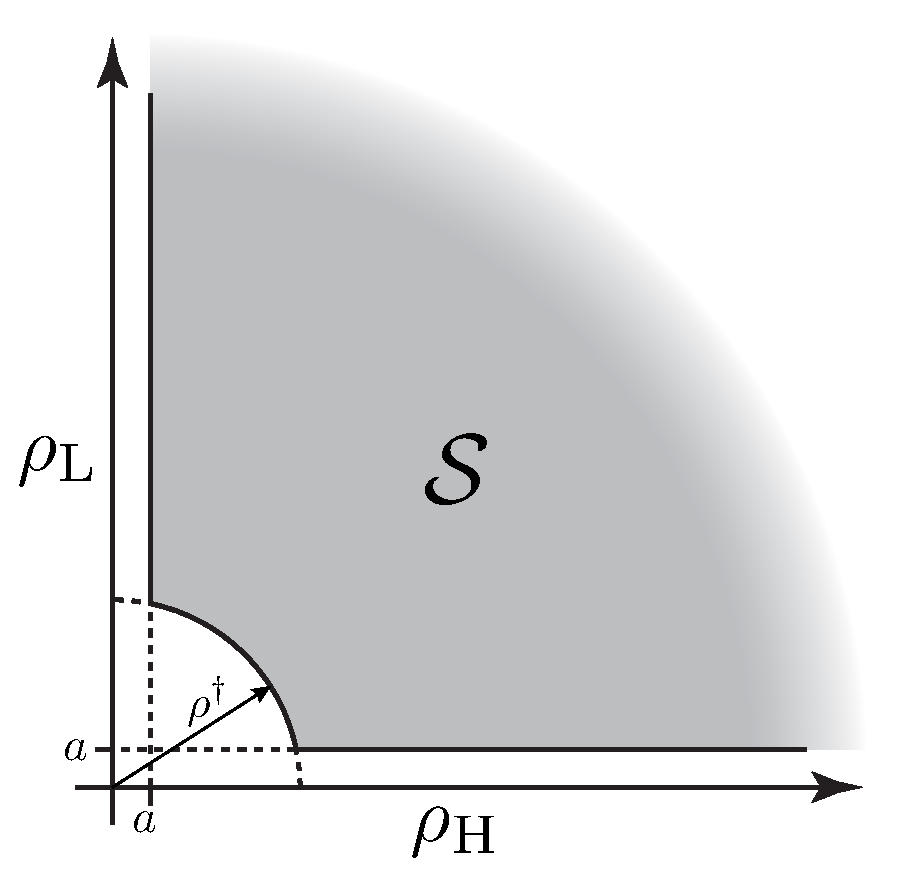
\includegraphics[height=4.25in]{figures/SNRintegrationRegion.pdf} \\
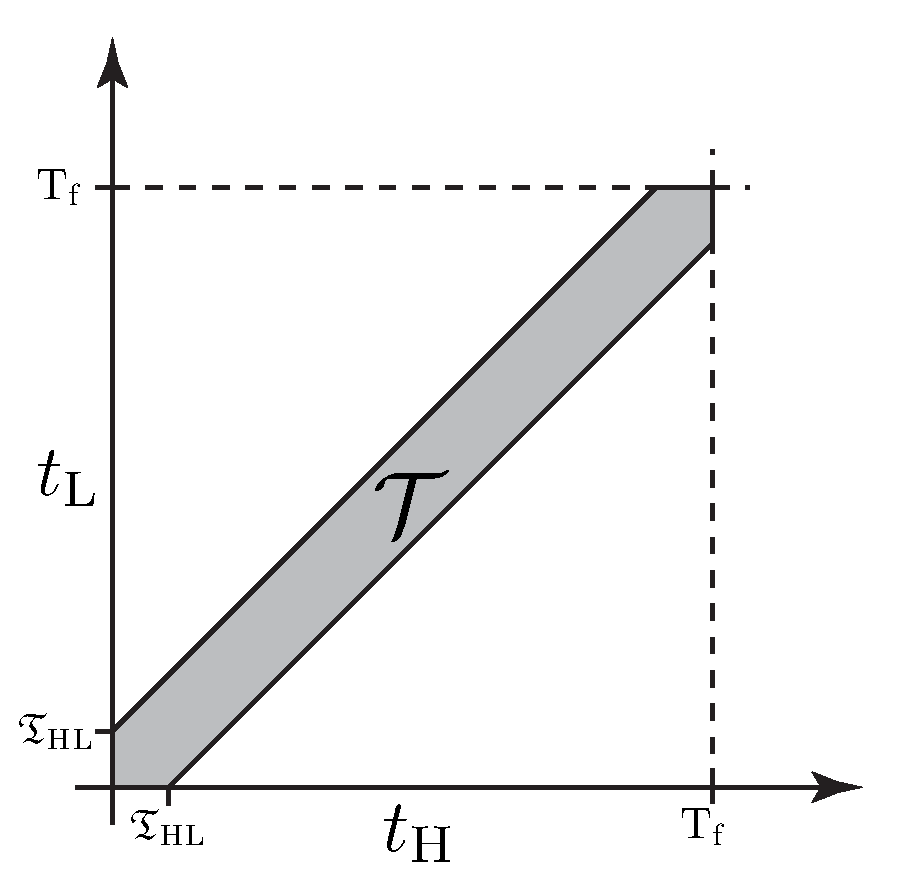
\includegraphics[height=4.25in]{figures/TimeIntegrationRegion.pdf}
\end{center}
\caption{The regions of integration in $\rho$, and time for a network of two detectors, $\varH$ and $\varL$.}
\end{figure}

\section{Computing Background Using Time Slides}
\label{sec:using_time_slides}

The first term in equation \ref{eqn:exampleSources} is the false alarm rate-density that we seek; thus, we could re-write the equation:
\begin{equation}
\tR_{\mathrm{all}}\left(\rho^\dagger \leq \sqrt{\rho_\varH^2 + \rho_\varL^2} \right) = \widetilde{\far}(\rho^\dagger) + \tR_{\mathrm{GW}}\left(\rho^\dagger \leq \sqrt{\rho_\varH^2 + \rho_\varL^2} \right)
\end{equation}
When we do an experiment and perform the coincidence test, we get a measure of $\tR_{\mathrm{all}}$. To get $\widetilde{\far}$ we must separate out the \ac{GW} terms. Unfortunately, we cannot tell the difference between a coincident trigger that came from noise and one that came from a gravitational wave. (If we could, we would not have to do any of this.) Thus, we must find other ways to separate the two. One way to do so is to perform a \emph{time slide}.

Consider what happens if we add a relative time offset to each detector's data-stream that is larger than the coincidence window between them. Doing so causes the gravitational wave triggers to become uncorrelated across the detectors. The rate of coincident noise triggers, however, is unaffected, since they were uncorrelated anyway. Thus, if we perform the same coincidence test on this ``slid" data as we did for the ``zero-lag" data, the expected number of coincidences is (assuming each detector only has one noise source):
\begin{equation}
\label{eqn:exptd_slid_coincs}
\Exptd \left(N_{\mathrm{all}} \left( \rho^{\dagger2} \leq \sum_{i=1}^{N_d}, \Tf, \vec{\mathcal{O}} \right) \right) = \vT(\Tf) \int_{\mathcal{S}} \prod_{i=1}^{N_d} \left( \rsrc_{i,\mathrm{noise}} P_{i,\mathrm{noise}}(\rho_i) + \rsrc_{\mathrm{GW}} P_{i,\mathrm{GW}}(\rho_i) \right) \d \rho_i
\end{equation}
Here we have made the dependence on the time offset explicit by defining an \emph{offset-vector}:

\begin{equation}
\label{eqn:offset_vec}
\vec{\mathcal{O}} = \left[0 ~~ \Delta t_2 ~~ \ldots ~~ \Delta t_{N_d} \right]
\end{equation}
(The offset for one of the detectors is always zero, since we are sliding the detectors with respect to each other.)

For example, in our two-detector case, the expected number of coincidences becomes:
\begin{eqnarray}
\label{eqn:slideTerms}
\lefteqn{ \Exptd\left(N_{\mathrm{all}} \left(\rho^{\dagger2} \leq \rho_\varH^2 + \rho_\varL^2, \Tf, \vec{\mathcal{O}} \right) \right) } \nonumber \\
 & = &  \vT(\mathrm{T_f}) \int_\mathcal{S}  \d \rho_\varH \d \rho_\varL \times \nonumber \\
 & & \left(\rsrc_{\varH,\mathrm{noise}}P_{\varH,\mathrm{noise}}(\rho_\varH) + \rsrc_{\mathrm{GW}}P_{\varH,\mathrm{GW}}(\rho_\varH)\right) \left(\rsrc_{\varL,\mathrm{noise}}P_{\varL,\mathrm{noise}}(\rho_\varL) + \rsrc_{\mathrm{GW}}P_{\varL,\mathrm{GW}}(\rho_\varL)\right) \nonumber \\ 
 & = & \coincT_{\varH\varL}(2\Tf - \coincT_{\varH\varL}) ( \rsrc_{\varH,\mathrm{noise}}\rsrc_{\varL,\mathrm{noise}} ~ \mathcal{I}_{\mathrm{H,noise; L,noise}} + \rsrc_{\varH,\mathrm{noise}}\rsrc_{\mathrm{GW}} ~ \mathcal{I}_{\mathrm{H,noise; L,GW}}  \nonumber \\
 & & ~ + ~ \rsrc_{\mathrm{GW}}\rsrc_{\varL,\mathrm{noise}} ~ \mathcal{I}_{\mathrm{H,GW; L,noise}} + \rsrc_{\mathrm{GW}}^2 ~ \mathcal{I}_{\mathrm{H,GW; L,GW}} ) 
\end{eqnarray}
where:
\begin{eqnarray}
\label{eqn:HnoiseLnoiseIntegral}
\mathcal{I}_{\mathrm{H,noise; L,noise}} & = & \frac{1}{2\pi \sigma_{\varH,\mathrm{noise}} \sigma_{\varL,\mathrm{noise}}} \int_{\mathcal{S}} e^{-(\rho_{\varH}^2 / 2\sigma_{\varH,\mathrm{noise}}^2 + \rho_{\varL}^2 / 2\sigma_{\varL,\mathrm{noise}}^2 )} \d \rho_{\varH} \d \rho_{\varL} \\
\label{eqn:HnoiseLgwIntegral}
\mathcal{I}_{\mathrm{H,noise; L,GW}} & = & \frac{4\pi \sigma_{\mathrm{GW}}^3}{(2.26)^3 \sqrt{2\pi} \sigma_{\varH,\mathrm{noise}}} \int_{\mathcal{S}} \rho_\varL^{-4} e^{-\rho_{\varH}^2 / 2\sigma_{\varH,\mathrm{noise}}^2} \d \rho_\varH \d \rho_\varL \\
\label{eqn:HgwLnoiseIntegral}
\mathcal{I}_{\mathrm{H,GW; L,noise}} & = & \frac{4\pi \sigma_{\mathrm{GW}}^3}{(2.26)^3 \sqrt{2\pi} \sigma_{\varL,\mathrm{noise}}} \int_{\mathcal{S}} \rho_\varH^{-4} e^{-\rho_{\varL}^2 / 2\sigma_{\varL,\mathrm{noise}}^2} \d \rho_\varH \d \rho_\varL \\
\label{eqn:HgwLgwIntegral}
\mathcal{I}_{\mathrm{H,GW; L,GW}} & = & \left( \frac{4\pi \sigma_{\mathrm{GW}}^3}{(2.26)^3} \right)^2 \int_{\mathcal{S}} \rho_\varH^{-4} \rho_\varL^{-4} \d \rho_\varH \d \rho_\varL
\end{eqnarray}
(Of the four, the only integral that can be solved analytically in region $\mathcal{S}$ is the GW/GW term\footnote{Note that if we did not impose the \ac{SNR} cut-off at $a$ then the GW/GW integral would give infinity; i.e., we would expect an infinite number of events in the detector from gravitational waves! This is a result of the model we have chosen for \acp{GW}. If the limits of integration were $\rho = 0,\infty$, then, from equation \ref{eqn:DtoRho}, we would be considering every source from here to infinity. By assuming that the distribution of sources is uniform throughout the universe (which we did by setting $\rsrc_{\mathrm{GW}}(\vec{\theta})$ to a constant), this means that if we look for an infinite distance, we will get an infinite number of sources --- a \ac{GW} version of Oblier's paradox \cite{obliers_paradox}. Of course, the real universe is not infinitely old; beyond $\sim 1\,\mathrm{Gpc}$ the number of \acp{CBC} begins to fall off \cite{rates_paper}. Further, we have assumed that the GW/GW term is independent of the noise. In practice, however, we do clustering, which couples these terms. Even if we had an ideal detector with stationary Gaussian noise in \ac{SNR}, below some \ac{SNR} the noise triggers would effectively cluster away all \ac{GW} events, even if the universe was infinitely old. We get around both of these difficulties by assuming that the \ac{SNR} cutoff is high enough that these effects do not affect our model (which, with $a=5.5$, is valid for both enhanced and advanced \ac{LIGO}.}, which is:
\begin{eqnarray}
\lefteqn{ \mathcal{I}_{\mathrm{H,GW;L,GW}} = } \nonumber \\
 & & \left( \frac{4\pi \sigma_{\mathrm{GW}}^3}{(2.26)^3} \right)^2 \left( \frac{\rho^{\dagger2} - 2a^2}{18 \rho^{\dagger6} a \sqrt{\rho^{\dagger2} - a^2}} \left( 1 + \frac{\rho^{\dagger4}}{8a^2\left(\rho^{\dagger2} - a^2 \right)} \right) + \frac{1}{9a^3 \left(\rho^{\dagger2} - a^2 \right)^{3/2}} \right)
\end{eqnarray}
if $\rho^\dagger \geq \sqrt{2}a$;
\begin{equation}
\mathcal{I}_{\mathrm{H,GW;L,GW}} = \left( \frac{4\pi \sigma_{\mathrm{GW}}^3}{(2.26)^3} \right)^2 \frac{1}{9a^6}
\end{equation}
otherwise. The other three integrals can be solved numerically, however; see Chapter \ref{ch:future_developments} for details.)

By de-coupling the gravitational waves in each detector, the GW/GW term is now much smaller than in the zero-lag case. For example, we can calculate the expected number of GW/GW coincidences for a $1.4/1.4\,\Msun$ binary neutron star system in each case. From \cite{rates paper}, the rate of \ac{BNS} coalescences in the universe is $\rsrc_{\mathrm{GW}} = 1 \times 10^{-6} \Mpc^{-3}\,\mathrm{yr}^{-1}$. During enhanced \ac{LIGO}, the $4\,\mathrm{km}$ \ac{LIGO} interferometers had a peak horizon distance to \ac{BNS} systems of $\sim40\Mpc$, which gives a sensitivity of $\sigma_{\mathrm{GW}} = \rho D_{\mathrm{horizon}} = 8 \times 40\Mpc = 320\Mpc$. Thus, if our two hypothetical detectors had the same sensitivity, then in one year we would expect:

\begin{eqnarray}
\Exptd\left( N_{\mathrm{GW}} \left( \rho^{\dagger}  =  11.3, \Tf = 1 \,\mathrm{yr} \right)\right) & = & \frac{4}{3} \pi \frac{\sqrt{2} (320\Mpc)^3}{(2.26)^3 (11.3 / \sqrt{2})^3} (1 \times 10^{-6}\Mpc^{-3}\,\mathrm{yr^{-1}}) (1\,\mathrm{yr}) \nonumber \\
 & = & 0.03 \nonumber
\end{eqnarray}
gravitational-wave events in zero-lag at a New \ac{SNR} of $8$ in each detector (which corresponds to a combined New SNR of $\rho^\dagger = \sqrt{2} \times 8 = 11.3$). In contrast, the expected number of coincident gravitational-waves in a one year-long time slide would be:

\begin{eqnarray}
\lefteqn{\Exptd\left( N_{\mathrm{GW}} \left(\rho^{\dagger} = 11.3, \Tf = 1\,\mathrm{yr}, \mathcal{O} \right) \right) } \nonumber \\
& = & (3.2 \times 10^{-10}\yr) ( 2\yr - 3.2\times10^{-10}\yr ) (1\times10^{-6}\Mpc^{-3}\yr^{-1})^2 \mathcal{I}_{\mathrm{H,GW;L,GW}}(\rho^\dagger = 11.3, a = 5.5) \nonumber \\
& = & 6 \times 10^{-13} \nonumber
\end{eqnarray}
Here, we have a coincidence window of $\coincT_{\varH\varL} = 10\,\mathrm{ms} \approx 3.2\times10^{-10}\yr$. This is about the light-travel time between Hanford and Livingston.

As can be seen in equation \ref{eqn:slideTerms}, doing the time slide has introduced mixing terms between \acs{GW} and noise. However, evaluating the integrals \ref{eqn:HnoiseLnoiseIntegral}--\ref{eqn:HgwLnoiseIntegral} requires fitting to data in order to determine $\sigma_{i,\mathrm{noise}}$ and $\rsrc_{i,\mathrm{noise}}$. Here we will assume the noise/GW terms are small relative to the noise/noise term, using the fact that number of expected gravitational waves in enhanced \ac{LIGO} is less than one as our reasoning. For a further discussion of the effect of these mixing terms, see Chapter \ref{ch:future_developments}.

Since the noise/noise term is the dominate source in a time-slide, we have:
\begin{equation}
\label{eqn:valid_slide_condition}
\tR_{\mathrm{all}}\left(\rho^{\dagger2} \leq \sum_{i=1}^{N_d} \rho_i^2, \mathcal{O} \right) \approx \widetilde{\far}(\rho^\dagger)
\end{equation}
Thus, we can measure the false alarm rate of a trigger with combined New \ac{SNR} $\rho^\dagger$ by simply performing a time slide, counting the number of coincidences that have a combined New \ac{SNR} $\geq \rho^\dagger$, and dividing by the slide duration. This method has the further advantage that we can perform multiple slides with the same data to improve our measurement of $\widetilde{\far}$. If we change the offset of each detector by enough to consider every slide to be independent --- i.e., we slide the data enough so that no two events can be coincident in more than one slide ---  then, from equation \ref{eqn:avg_rate_param}, in $N_t$ slides:

\begin{equation}
\label{eqn:meanFAR1}
\overline{\far}(\rho^\dagger) = \frac{\sum_{k=1}^{N_t} \widehat{N}_k \left(\rho^{\dagger2} \leq \sum_{i=1}^{N_d} \rho_i^2 \right)}{\Tb} 
\end{equation}
where $\widehat{N}_k \left(\rho^{\dagger2} \leq \sum_{i=1}^{N_d} \rho_i^2 \right)$ is the measured number of coincidences with a combined New \ac{SNR} $\geq \rho^\dagger$ in the $k\th$ slide, and $\Tb$ is the total \emph{background time}. The background time is the sum of the length of each slide; the length of each slide is the intersection of every detector's foreground analysis time after they have been slid. Therefore:

\begin{equation}
\label{eqn:tBackground}
\Tb = \sum_{k=1}^{N_t} \left| \left( \mathbb{T}^A + \mathcal{O}_k[A] \right) \bigcap \left( \mathbb{T}^B + \mathcal{O}_k[B] \right) \bigcap \ldots \bigcap \left( \mathbb{T}^{N_d} + \mathcal{O}_k[N_d] \right) \right|
\end{equation}
(Here, $\mathbb{T}^i$ is the analysis segment of the $i\th$ detector; $\left| \mathbb{T}^i \right| = \Tf^i$.) With a finite data set, a single \emph{linear} slide will not have the same duration as the foreground time since the overlap between detectors will decrease with increasing offsets. If the slide is done on a \emph{ring}, so that data that is slid past the end of the segment is put at the beginning, than a slide will have the same duration as the zero-lag. However, if there are gaps in the data, then even sliding on a ring will result in different durations from slide-to-slide, since the gaps will align differently in each slide. We therefore define the \emph{effective number of slides}, $\widetilde{N}_t$, as the ratio of the total background time to the foreground time:
\begin{equation}
\label{eqn:effective_Nslides}
\widetilde{N}_t \equiv \frac{\Tb}{\Tf}
\end{equation}
so that equation \ref{eqn:meanFAR1} can be written:
\begin{equation}
\label{eqn:meanFAR2}
\overline{\far}(\rho^\dagger) = \frac{\widehat{N}_{\mathrm{total}} \left(\rho^{\dagger2} \leq \sum_{i} \rho_i^2 \right)}{\Tf \widetilde{N}_t} = \frac{\overline{N} \left(\rho^{\dagger2} \leq \sum_{i} \rho_i^2 \right)}{\Tf}
\end{equation}
Since the sum over the number of slides in the numerator of equation \ref{eqn:meanFAR1} is simply a sum of counts, here we have written it as $\widehat{N}_{\mathrm{total}} \left(\rho^{\dagger2} \leq \sum_{i} \rho_i^2 \right)$, which is the total number of triggers with combined New \ac{SNR} $\geq \rho^\dagger$ (\emph{false alarms}) in all the slides. Thus, $\overline{N} \left(\rho^{\dagger2} \leq \sum_{i} \rho_i^2 \right)$ is the average number of false alarms in a single experiment with a duration equal to $\Tf$. Since this is the mean of a stationary Poisson process, from equation \ref{eqn:err_R}, the error in $\overline{\far}$ is:
\begin{eqnarray}
\label{eqn:err_FAR}
\delta \overline{\far}(\rho^\dagger) & = & \frac{1}{\Tf} \sqrt{\frac{\overline{N} \left(\rho^{\dagger2} \leq \sum_{i} \rho_i^2 \right)}{\widetilde{N}_t}} \nonumber \\
 & = & \frac{1}{\Tf} \sqrt{\frac{\widehat{N}_{\mathrm{total}} \left(\rho^{\dagger2} \leq \sum_{i} \rho_i^2 \right)}{\widetilde{N}_t^2}} \nonumber \\
 & = & \frac{\sqrt{\widehat{N}_{\mathrm{total}} \left(\rho^{\dagger2} \leq \sum_{i} \rho_i^2 \right)}}{\Tb}
\end{eqnarray}

We have arrived at a way to calculate false alarm rates for a single template: perform the coincidence test in several times slides; compute the duration of each time slide; count the number of slide coincidences in all slides that have a combined New \ac{SNR} greater-than-or-equal to a given foreground New \ac{SNR}; divide by the total background time.

\section{Computing FARs with Multiple Templates}
\label{sec:mulitple_templates}

To compute a false alarm rate across a bank of templates, we would replace the time integral in equation \ref{eqn:N_general_prob} with an integral over the template parameters, $\{\vartheta_m\}$, bounded by the ethinca ellipsoid at $\rho$, $\mathcal{E}(\rho)$:

\begin{equation}
\Exptd\left(N_{\mathrm{uncorr}}\left(\rho^{\dagger2} \leq \sum_i\rho_i^2, \Tf \right)\right) = \int_{\mathcal{S}(\rho^\dagger)} \int_{\mathcal{E(\rho)}} \prod_i^{N_d} \sum_j^{N_s}  \prod_{m}^{n_p} \rsrc_{i,j} P_{i,j}(\rho_i, \{\vartheta_m \}) \d \vartheta_m \d t_i \d \rho_i
\end{equation}
where $n_p$ is the number of parameters used. For example, in a non-spinning search in which the templates are laid out in $\tau_0$ and $\tau_3$ space, this would be:
\begin{equation}
\Exptd\left(N_{\mathrm{uncorr}}\left(\rho^{\dagger2} \leq \sum_i\rho_i^2, \Tf \right)\right) = \int_{\mathcal{S}(\rho^\dagger)} \int_{\mathcal{E(\rho)}} \prod_i^{N_d} \sum_j^{N_s}  \rsrc_{i,j} P_{i,j}(\rho_i, \tau_0, \tau_3) \d \tau_0 \d \tau_3 \d t_i \d \rho_i
\end{equation}

Ideally, the probability of getting a trigger would be independent of the template parameters. In that case, the integral over $\mathcal{E}(\rho)$ could be carried out independent of the source \acp{PDF}, as was done with the time integral in section \ref{sec:coincidence_modelling}. This would mean that the number of coincident triggers with a combined New \ac{SNR} $\geq$ to any given value would only be dependent on $\rho$. This is ideal, since the false alarm rate is meant to be a measure of how likely a trigger is a gravitational wave, independent of parameters. It would also mean that we could simply count the number of slide coincidences to get the false alarm rate, as described above, without needing any correction for the parameters of the templates.

In practice, however, the false alarm rate of a template \emph{is} dependent on its parameters. Figure \ref{fig:newsnr_v_mchirp} shows the dependence of the cumulative rate of coincident slide triggers on chirp mass ($\mathcal{M}$) when the rates are based on New \ac{SNR}. These triggers were taken from $100$ slides in six weeks (about $0.03\,\mathrm{yr}$ of analysis time) of enhanced \ac{LIGO} data in which the $4\,\mathrm{km}$ Hanford (H1) and Livingston (L1) detectors were analyzed (``S6"; see Chapter \ref{ch:s6_results} for details). As can be seen in Figure \ref{fig:newsnr_v_mchirp-a}, the overall rate of triggers decreases with increasing chirp mass. This is due to the fact that the template bank is more sparsely populated at higher masses. Conversely, the variance of the rate of triggers roughly increases with increasing mass, leading to a higher rate of high New \ac{SNR} triggers at high mass. This occurs because the inspiral phase of a higher-mass template spends less time in band compared to lower masses. As a result, $\chi^2$ does a poorer job distinguishing high mass \acp{CBC} from glitches, which also tend to ring off the higher masses with larger \ac{SNR}.

The joint effect of the lower overall rate and higher variance of high-mass templates can be seen in Figure \ref{fig:newsnr_v_mchirp-b}, which plots the combined New \ac{SNR} of the triggers versus chirp mass. (To go from \ref{fig:newsnr_v_mchirp-a} to \ref{fig:newsnr_v_mchirp-b}, think of the color bar as the z-axis, and imagine rotating the axes so that $x \rightarrow y$, $y \rightarrow z$, and $z \rightarrow x$.) Due to the decrease in the overall rate, the cumulative rate drops off with increasing chirp mass at low combined New \ac{SNR} (orange -- yellow lines in the figure). However, due to the higher variance, the rate increases with increasing chirp mass (up to the middle of the chirp-mass space, anyhow) at large combined New \ac{SNR} (the red line in the figure). This latter effect can be particularly problematic since we are most interested in triggers with higher New \ac{SNR}. For example, consider what were to happen if a binary neutron star template with $\mathcal{M} = 2\,\Msun$ rang off with a New \ac{SNR} of 10.5. If our template bank was restricted to binary neutron stars ($\mathcal{M} \approx 1$--$3\,\Msun$), the trigger would stick well above background, as can be seen in Figure \ref{fig:newsnr_v_mchirp-b}. However, if we include the entire bank in the false alarm calculation, then the event would be out-ranked by the two events between $\mathcal{M} = 7$--$9\,\Msun$, leading to a $\far \approx 50\,\mathrm{yr}^{-1}$. This high \ac{FAR} would have more to do with our ranking statistic's inability to take into account the parameters of the template than with our degree of belief in how likely the trigger is a gravitational wave.

One way to fix this is to break up the chirp-mass space when computing \acp{FAR}. If we bin the space such that the cumulative rate is roughly constant for a given New \ac{SNR} across the bin, then we can use our naive approach of counting slide triggers to get $\far$. The $\far$ computed in each bin, however, is not the true \ac{FAR} for the search, since we sliced up the parameter space in order to arrive at it. To understand why the slicing needs to be accounted for, consider the number of bins. Our initial choice of bins was arbitrary: we could choose to slice the parameter space up even more; in so doing, we would get a smaller $\far$. Yet this plummeting \ac{FAR} would have little to do with the likelihood that the triggers are gravitational waves and everything to do with our choice of bins. Thus, to fix this, we must compute a \emph{combined \ac{FAR}}, $\cfar$, across all of the bins.

In order to compute a combined \ac{FAR}, we use the \emph{uncombined} \ac{FAR} --- i.e., the \acp{FAR} computed using the bins --- as our ranking statistic. This means we must compute an uncombined \ac{FAR} for the slide triggers. We do this in the same manner that we compute uncombined \acp{FAR} for zero-lag triggers: we count the number of slide triggers that have a combined New \ac{SNR} $\geq$ the $\rho$ of a given trigger. By doing so we treat a given slide as if it were zero-lag. Thus, we do not include the slide in which we are computing uncombined \acp{FAR} in the background estimate for that slide. Since we use one-less slide for measurement of the background triggers' \acp{FAR}, the error in our measurement of the slide triggers \acp{FAR} will be larger than that of zero-lag triggers. Assuming each slide has roughly the same duration then, from equation \ref{eqn:err_FAR}, the error is increased to:

\begin{equation}
\label{eqn:err_FAR_slide}
\delta \overline{\far}_{\mathrm{slide}} \approx \frac{\sqrt{ \widehat{N}_{\mathrm{total}} ( 1 - \widetilde{N}_t^{-1} ) }}{ \Tb (1- \widetilde{N}_t^{-1}) }
\end{equation}
For large $N_t$, however, the discrepancy between the zero-lag and time-slide $\delta \far$ is small. 

Once we have uncombined \acp{FAR} for both foreground and background triggers, we compute the combined \acp{FAR} by counting the total number of triggers with a $\far$ \emph{less-than} the given trigger's \ac{FAR}, $\far^\dagger$:

\begin{equation}
\label{eqn:cfar_1}
\overline{\cfar}( \far^\dagger ) = \frac{ \widehat{N}_{\mathrm{total}}\left( \far < \far^\dagger \right) }{\Tb}
\end{equation}
The reason we count the number of triggers that have a \ac{FAR} \emph{less-than} and not \emph{less-than or equal-to} $\far^\dagger$ can be understood by considering what happens to a trigger that has a $\rho$ larger than all the background in its bin. If a trigger is louder than all the background, it will have a measured \ac{FAR} of 0. This does not mean we are absolutely certain the trigger is a gravitational wave. A \ac{FAR} of 0 means that we have set an upper-limit on the true \ac{FAR} to be less-than $1/\Tb$, within the error bars; i.e.:

\begin{equation}
\label{eqn:zeroFAR}
\overline{\far}(\rho^\dagger) = 0 \Rightarrow \widetilde{\far}(\rho^\dagger) < \frac{1}{\Tb} \pm \frac{1}{\Tb}
\end{equation}
Since we have only placed an upper limit on the uncombined \ac{FAR}, we should also only be able to place a limit on the combined \ac{FAR}; thus, if we got zero for $\far^\dagger$ we should also get zero for $\cfar^\dagger$. (The combined \ac{FAR} limit will be higher however; specifically, it will be $N_{\mathrm{bins}}/\Tb$, where $N_{\mathrm{bins}}$ is the number of bins.) Yet if we have, say, $N_0$ triggers in the background with $\far = 0$ and we were to count the number of triggers $\leq \far^\dagger$, we would get a combined \ac{FAR} \emph{equal} to $N_0/\Tb$, not less-than. Thus, we would have extracted a measured value for the combined \ac{FAR} from a limit, without having had any new information about the trigger.

Breaking up the parameter space into bins and computing combined \acp{FAR} from uncombined allows us to map the triggers onto a space where the parameter dependence has been removed. Note, however, that since a slide is not counted against itself, in each bin we will have at least one trigger with $\overline{\far} = 0$. This is the trigger that has the largest value of $\rho$; i.e., it is the loudest background trigger. (We could have more than one slide trigger in a bin with $\overline{\far} = 0$ if a single slide contained multiple triggers that were louder than the triggers in all other slides.) Thus, if we have $N_{\mathrm{bins}}$ bins, we will have at least $N_{\mathrm{bins}}$ background triggers with $\overline{\far} = 0$. This means that if a foreground trigger has $\overline{\far} = 1/\Tb$ in its bin, it will have $\overline{\cfar} = N_{\mathrm{bins}}/\Tb$. In other words, even if a foreground trigger has a $\rho$ that is far larger than all but one slide trigger, and that slide trigger is in the same bin, its combined \ac{FAR} will increase by at least a factor of $N_{\mathrm{bins}}$. If a trigger has a zero uncombined \ac{FAR} (and therefore a zero combined \ac{FAR}), the smallest upper limit that can be placed on its true false alarm rate will also increase according to the number of bins, or \emph{trials factors}. The number of bins should therefore be kept to a minimum.

Figure \ref{fig:ufar_v_mchirp} shows the background distribution in uncombined \ac{FAR} of the same set of triggers used in Figure \ref{fig:newsnr_v_mchirp}. The bins used are clearly visible via the ``steps" in Figure \ref{fig:ufar_v_mchirp-b}. These bins --- which are $\mathcal{M}/\Msun \in \{ [0.0, 3.48); [3.48, 7.4); [7.4,\infty) \}$ --- are the same that were used in the analysis of LIGO's fifth and sixth science runs (S5 and S6, respectively). As can be seen by the lines of constant high cumulative rate in Figure \ref{fig:ufar_v_mchirp-b} (orange -- yellow lines), the bins are not sufficient to make the rate completely independent of the mass. Indeed, this is impossible with any choice of bins, since there are simply not enough triggers at high mass to extend the high cumulative rate lines into that region. However, for \emph{low} cumulative rates, the space has been sufficiently ``flattened." Note, in particular, the red line, which shows a cumulative rate of $1/\Tb$ in each bin. In Figure \ref{fig:newsnr_v_mchirp-b}, this line dropped off at low chirp mass, which would cause low-mass systems to get higher-than-expected false alarm rates, as in the case of the \ac{BNS} system above. Now, low-mass systems with high $\rho$ are ranked on par with the medium mass systems. Since these are the triggers we are most interested in, this choice of bins is sufficient for our purposes, and we have only incurred a trials factor of 3.

There is one last parameter that we need to be aware of when choosing the number of bins: the number of detectors contributing to the coincidence. Since combined New \ac{SNR} is computed by taking the quadrature sum of the single-\ac{IFO} New \acp{SNR}, coincidences that have a larger number of contributing detectors will have a larger combined $\rho$. For example, if we analyze three detectors --- call them H, L, and V --- then we can have four types of coincidences: HL, HV, LV, and HLV. A trigger with New \ac{SNR} $= 8$ in each detector will have a combined New \ac{SNR} $= \sqrt{2}\times8$ if it is a HL, HV, or LV coincidence, and a combined New \ac{SNR} $= \sqrt{3}\times8$ if it is a triple coincidence. That may seem appropriate: after all, the more detectors that observe the event, the more likely we are to believe it to be a \ac{GW}. However, due to the antenna pattern of the detectors, and the fact that they are not co-located nor have the same sensitivity, a \ac{GW} will not be seen in all detectors if it came from a source in certain sky locations and orientations. If we were to compute \acp{FAR} without first binning the triggers by the number of coincident triggers, or \emph{coincidence type}, we would subtly introduce a location and orientation bias into the \ac{FAR}. To avoid this, we also bin triggers by their coincidence type.\footnote{Admittedly, simply binning the triggers by coincidence type then using the uncombined \acp{FAR} to get the combined \ac{FAR} is not the perfect solution to remove biases either. Doing so treats all the coincidence types with equal weight. However, if the detectors have varying sensitivities, it is more likely to get a gravitational wave from coincidences of the most sensitive detectors. A better approach would be to add some weight to each coincidence type that is proportional to the sensitivity of the constituent detectors before combining the \acp{FAR}. The same argument applies to mass-bins: if the detectors are more sensitive to certain parameter ranges, we should weight accordingly. A likelihood-based weighting that attempted to remedy these concerns was used in the joint LIGO-Virgo search in the last few months of \ac{S5}; see \cite{ref:LVC_paper} for details. For the rest of \ac{S5} and \ac{S6}, the detectors' sensitivities were roughly on-par with each other, so the simpler equal-weight method described here was used.}

Across the course of an analysis period varying combinations of detectors will be available to analyze. (An \ac{IFO} is not analyzable if it is not in \emph{Science} mode, which can occur if it ``loses lock"; see Chapter \ref{ch:ihope_pipeline} for details.) For example, in the three detector case given above, we can have four different \emph{instrument times}: periods when HLV were on, and periods when HL, HV, or LV were on. Obviously, only certain coincident types can occur in a given period. Therefore, when computing a \ac{FAR} for a trigger, we should not include analysis times in which it was impossible for the coincidence type of the trigger to occur. If we did, we would artificially decrease the false alarm rate of the trigger. As a result, each of the various instrument times are treated as independent experiments: both uncombined and combined \acp{FAR} are computed within the instrument time, and \acp{FAR} are never calculated across instrument times. This also means that coincidences of the same type cannot be combined across instrument times. For example, in the three detector case, we can get HL, HV, and LV coincident triggers in both HLV time and each of the respective double-coincident times. However, there is a slight difference between the doubles in triple time and the doubles in double time. The double-coincident triggers in HLV time are triggers that were coincident with one other detector \emph{and not} coincident with the third detector. The doubles in double time, however, consist of triggers that would not have been coincident with the third detector \emph{and} triggers that would have been coincident, had the third detector been on. This latter set is clearly a larger population. Thus, if coincidence types were grouped across instrument times (using the sum of the instrument times for the analysis time), we would underestimate the \acp{FAR} of the triggers from double-time and overestimate the \acp{FAR} from triple-time.\footnote{We can, however, group coincidence-types together across instrument times if we reanalyze the data with the other detector removed, or \emph{vetoed}. For example, we can group HL triggers in HL time with HL triggers in HLV time if we re-analyzed the HLV data with V removed. This has been done occasionally in order to get a better estimate of double coincident triggers with low or zero \acp{FAR}.} 

Summarizing, the number of bins, or trials factors, that we use depends on how strongly the ranking statistic couples to a parameter and on the number of coincident types possible in the instrument time being analyzed. In the low-mass \ac{CBC} search we use three mass bins based on chirp mass. This means that we have a trials factor equal to $3$ during double-coincident instrument times. During triple-coincident instrument times in which all coincident types are used, this factor increases to 12 ($3$ mass-bins times $4$ possible coincidence types).

\begin{figure}[p]
\begin{center}
\subfigure[Cumulative Rate v. Combined New SNR. Each line represents the cumulative rate in one chirp-mass bin as a function of Combined New SNR, the boundaries of which are shown in (b).]{\label{fig:newsnr_v_mchirp-a}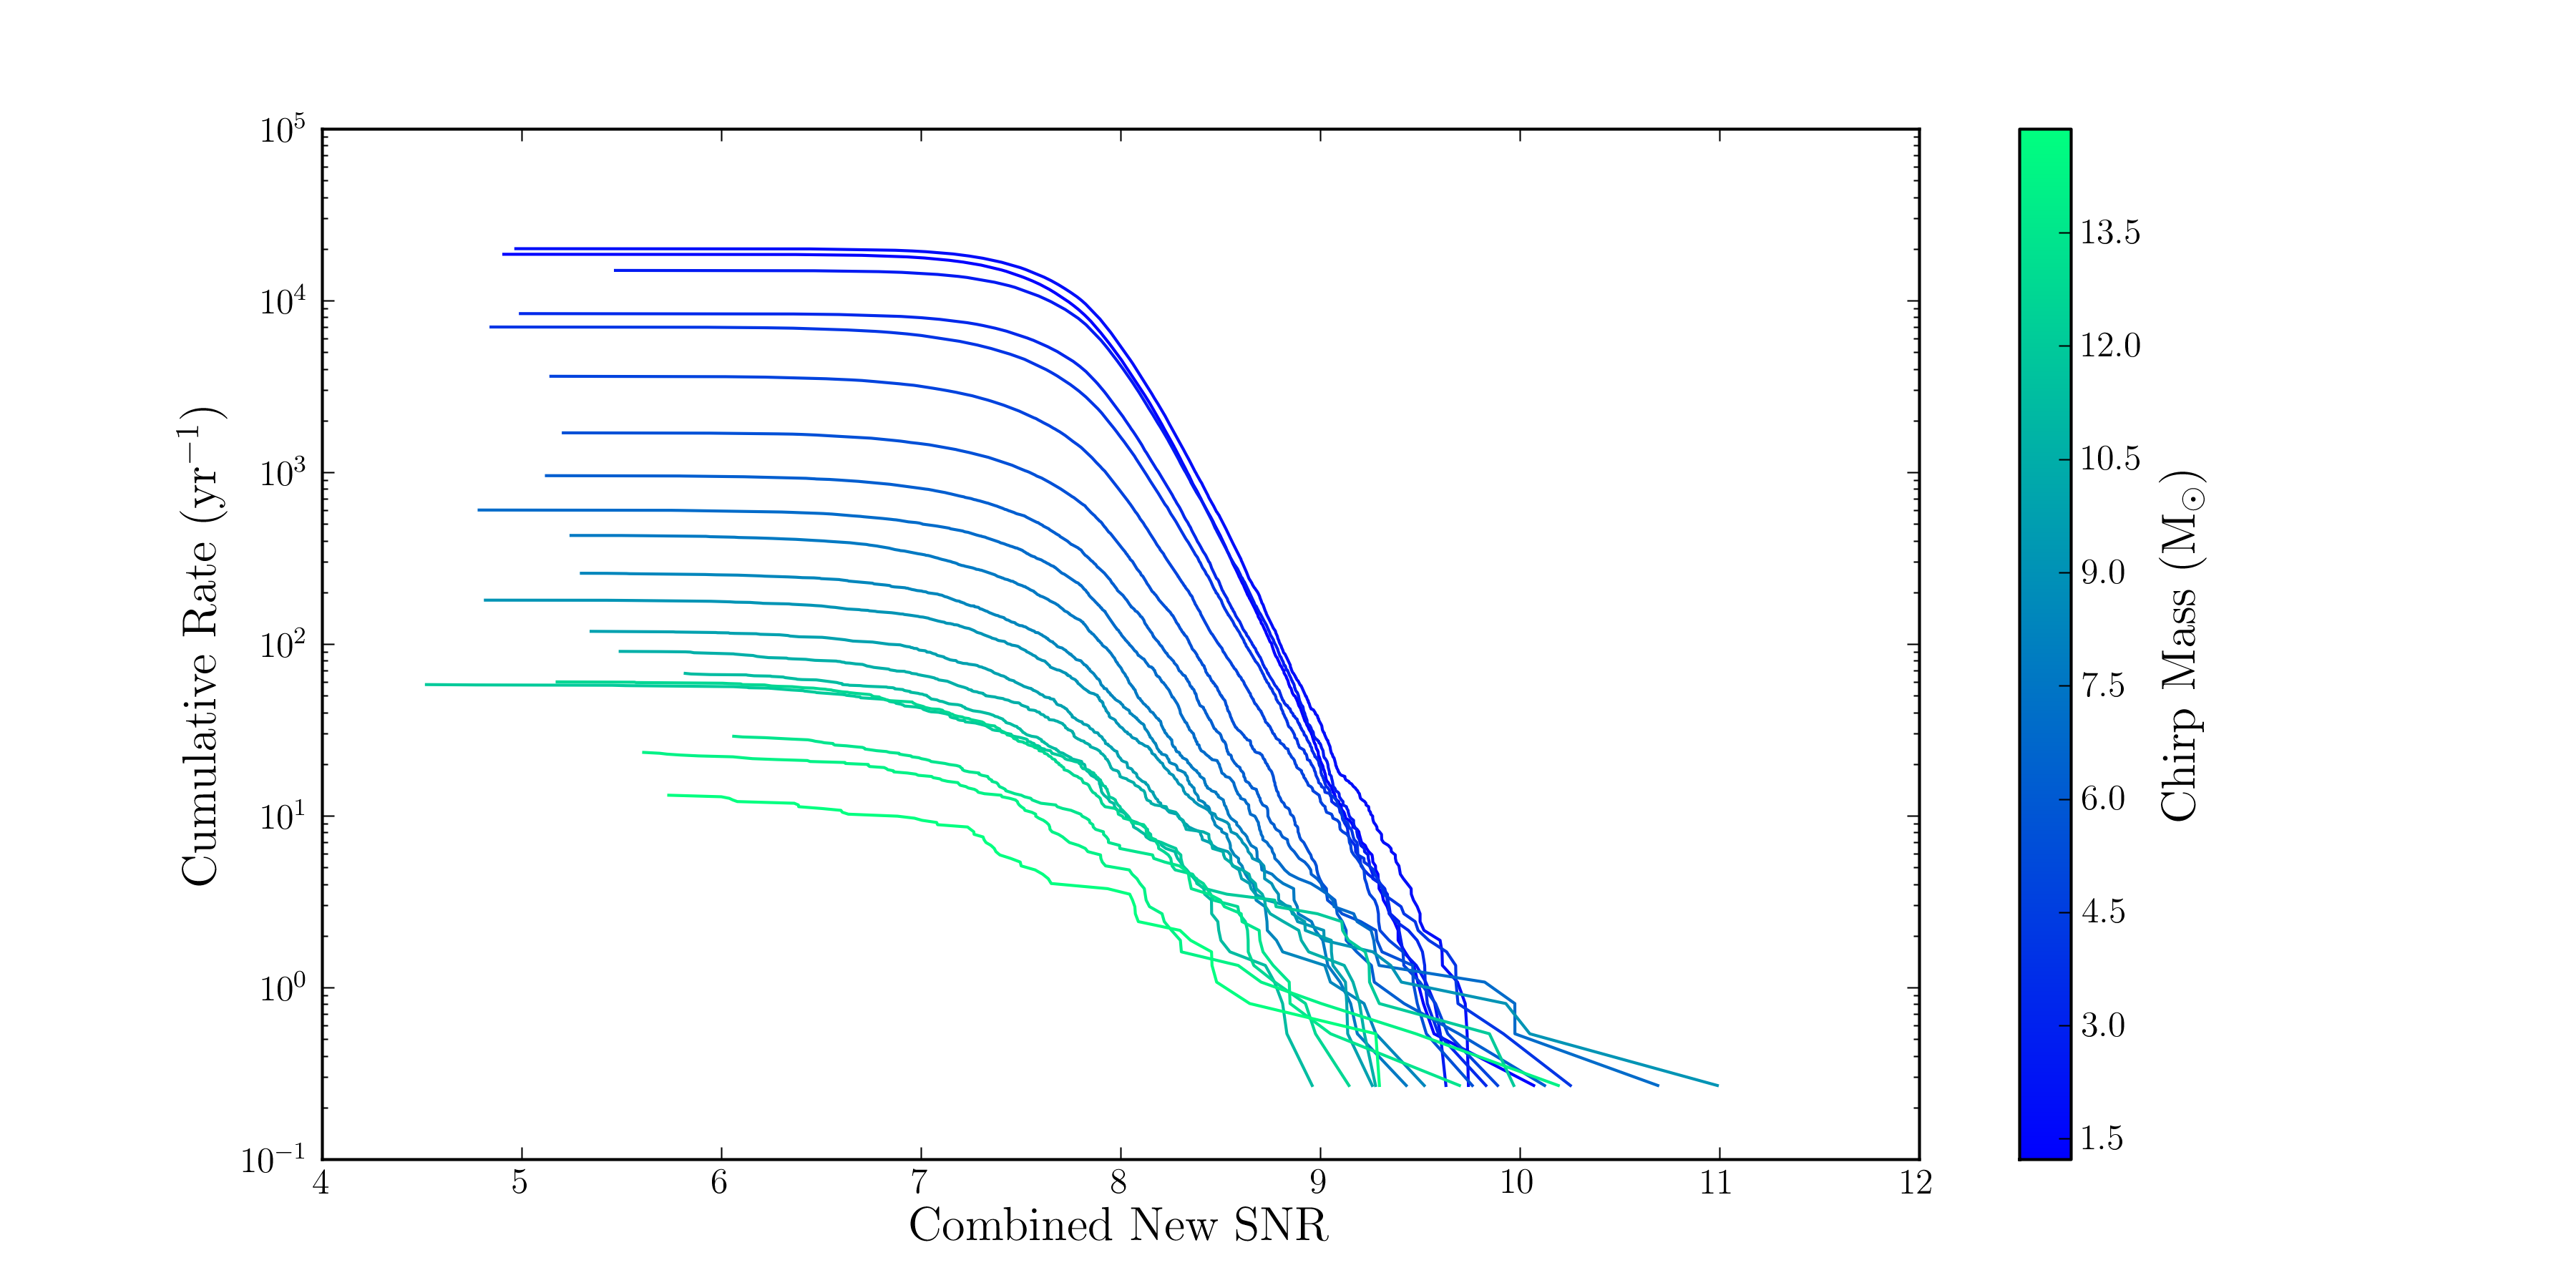
\includegraphics[width=6.5in]{figures/H1L1_H1L1-plotNdensity_cumnum_snr_vs_mchirp.png}}
\subfigure[New SNR v. Chirp Mass. Colored lines show lines of constant cumulative rates across the chirp-mass bins. Dashed lines show the bin boundaries used.]{\label{fig:newsnr_v_mchirp-b}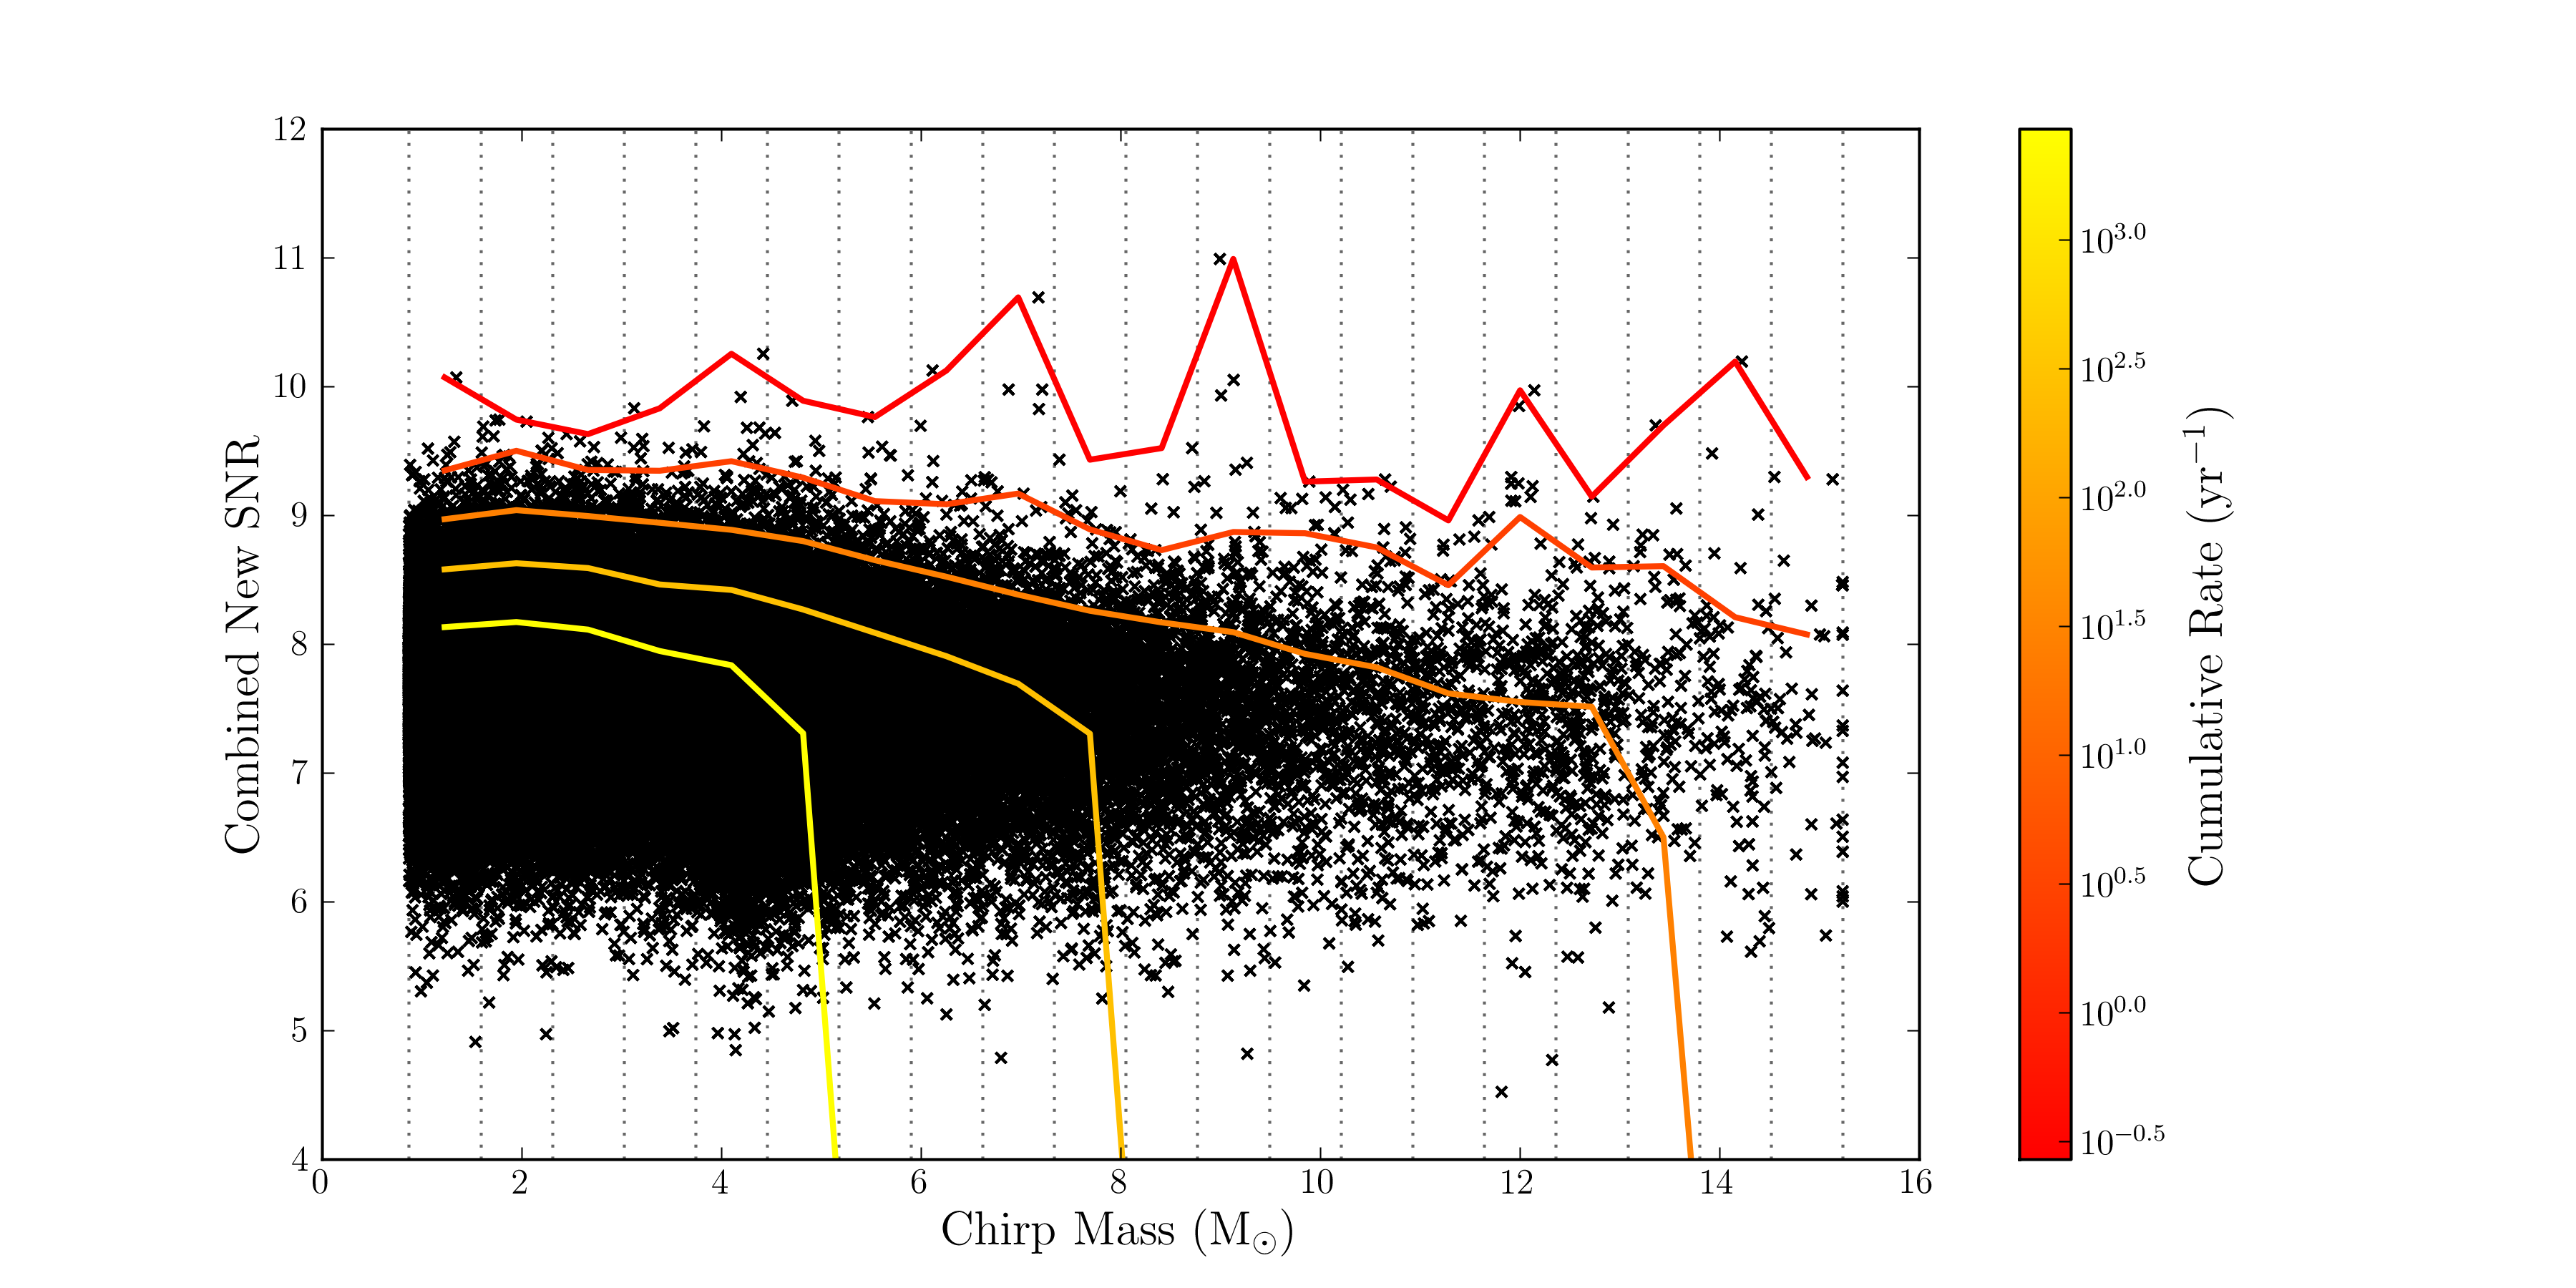
\includegraphics[width=6.5in]{figures/H1L1_H1L1-plotNdensity_snr_vs_mchirp.png}} \\
\end{center}
\caption{The rates of slide coincidences in equally-spaced chirp-mass bins as a function of Combined New SNR. Black crosses are coincident triggers taken from 100 slides in six weeks of enhanced \ac{LIGO} data. The cumulative rates (the y-axis in (a) and the color axis in (b)) are computed by counting the number of triggers with a Combined New SNR $\geq$ each trigger within each bin. Only the $4\,\mathrm{km}$ Hanford (H1) and Livingston (L1) triggers were analyzed during this time; as such, all coincidences are H1L1 triggers.}
\label{fig:newsnr_v_mchirp}
\end{figure}

\begin{figure}[p]
\begin{center}
\subfigure[Cumulative Rate v. Uncombined FAR. Each line represents the cumulative rate in one chirp-mass bin as a function of Uncombined FAR, the boundaries of which are shown in (b).]{\label{fig:ufar_v_mchirp-a}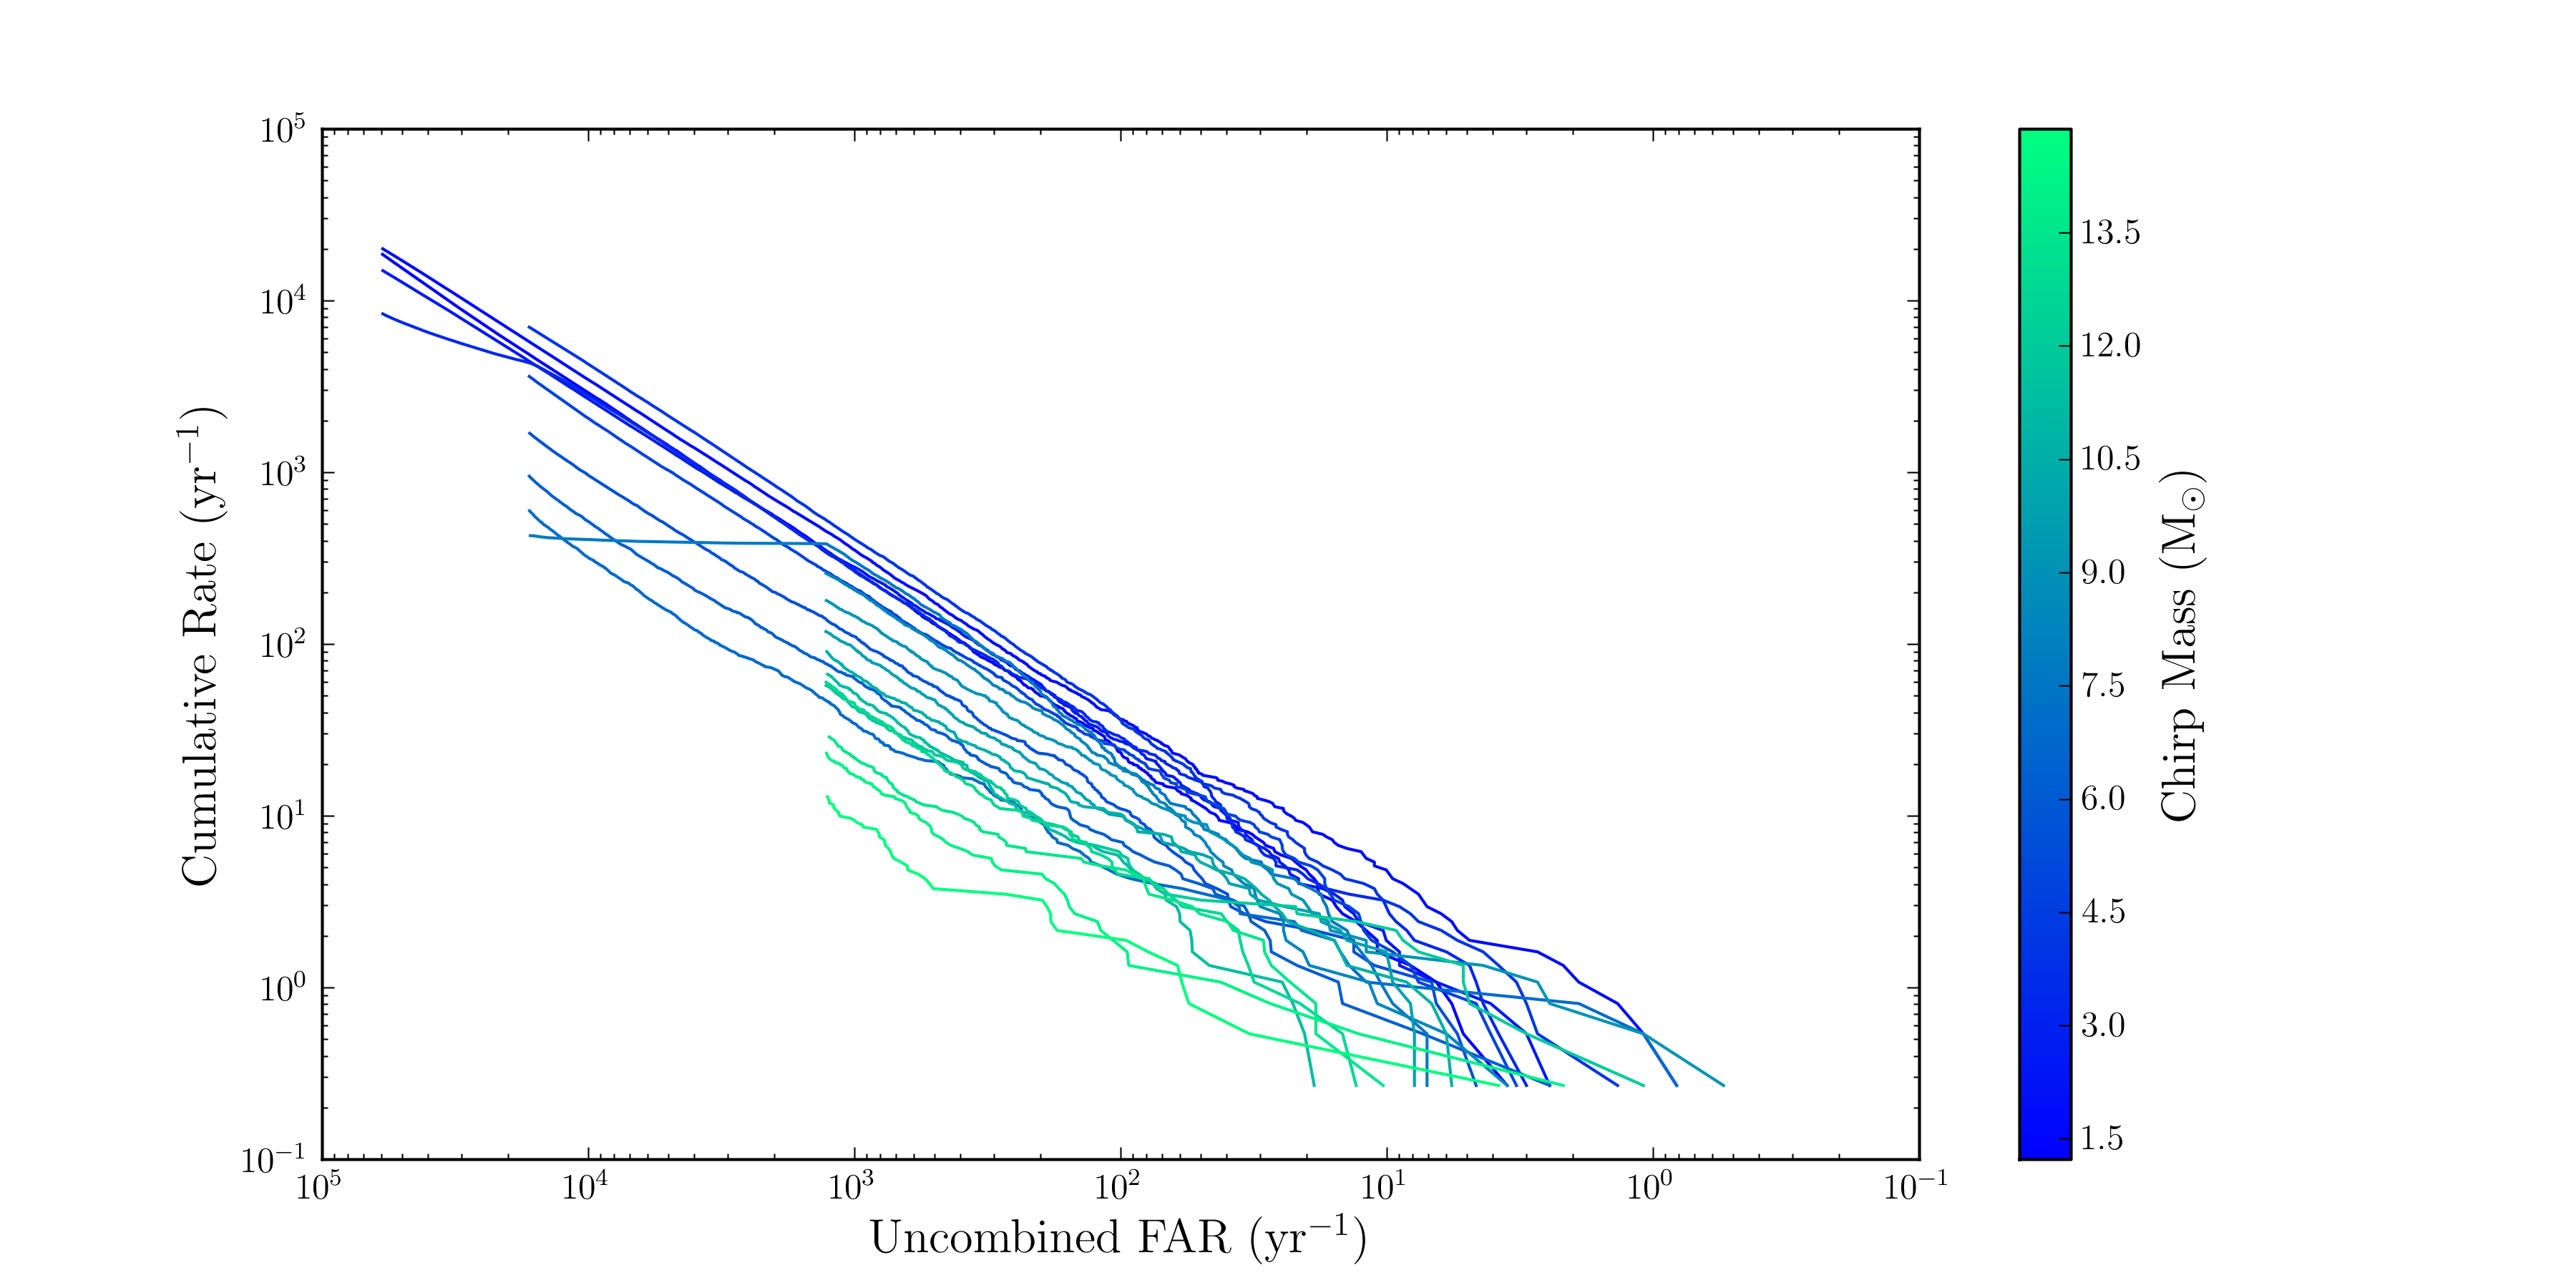
\includegraphics[width=6.5in]{figures/H1L1_H1L1-plotNdensity_cumnum_false_alarm_rate_vs_mchirp.png}}
\subfigure[Uncombined FAR v. Chirp Mass. Colored lines show lines of constant cumulative rates across the chirp-mass bins. Dashed lines show the bin boundaries used.]{\label{fig:ufar_v_mchirp-b}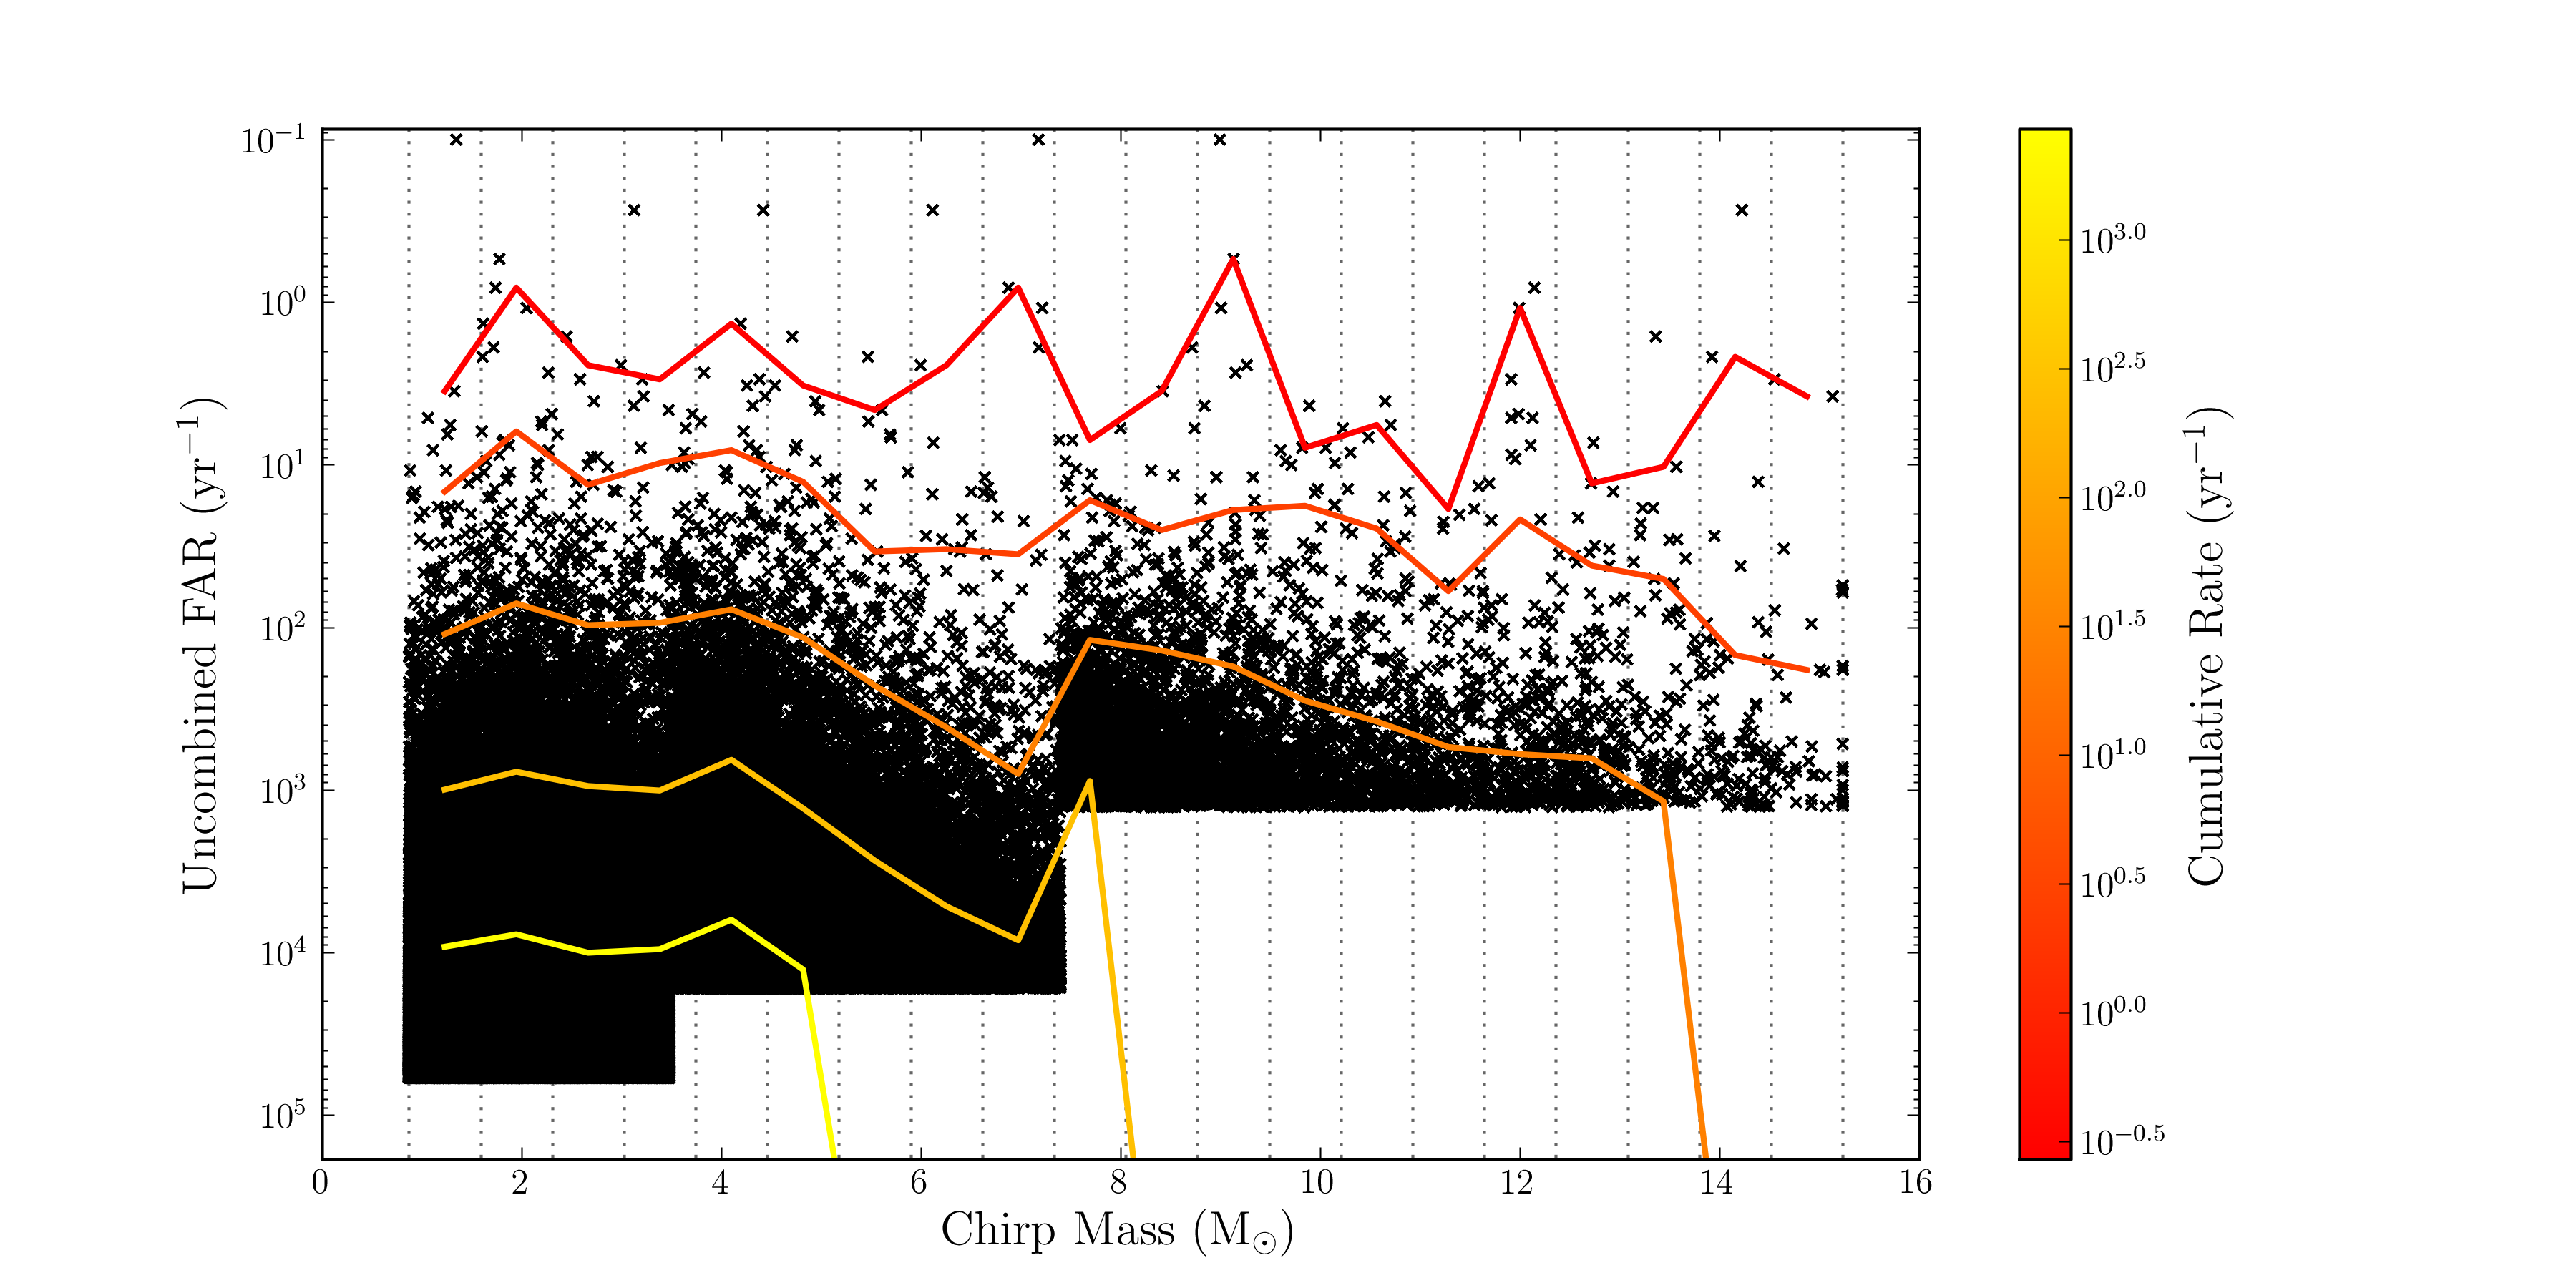
\includegraphics[width=6.5in]{figures/H1L1_H1L1-plotNdensity_false_alarm_rate_vs_mchirp.png}}
\end{center}
\caption{The rates of slide coincidences in various chirp-mass bins as a function of Uncombined \ac{FAR}. The data used is the same as that in Figure \ref{fig:newsnr_v_mchirp}. The bin boundaries used to compute the Uncombined \acp{FAR} are visible in the steps in seen in (b). The Uncombined \acp{FAR} were computed using \texttt{ligolw\_cbc\_cfar} using the same bins as used in the S5 and S6 searches (see Chapter \ref{ihope_pipeline} for details). The cumulative rates are computed by counting the number of triggers with an Uncombined \ac{FAR} $<$ each trigger within each bin. As a result the Uncombined \ac{FAR} axes are inverted. Also note that the Uncombined \ac{FAR} axes are plotted on a log scale.}
\label{fig:ufar_v_mchirp}
\end{figure}

\section{Alternate Method to Compute Combined FARs}
\label{sec:alternate_cfar_method}

There is an alternate, but equivalent, method to computing combined \acp{FAR} that does not require computing uncombined \acp{FAR} for all of the background triggers. We describe it here as it was used in the \ac{S5} search.

We begin by re-writing equation \ref{eqn:cfar_1} as an explicit sum over the number of triggers in each bin:

\begin{equation}
\label{eqn:cfar_2}
\overline{\cfar}( \far^\dagger ) = \frac{1}{\Tb} \sum_{p=1}^{N_{\mathrm{bins}}} \int_{0}^{\far^\dagger \Tb} \widehat{n}_p( \far' ) \d \far'
\end{equation}
Here, $\widehat{n}_p( \far' )$ is the measured number of triggers in $p\th$ bin with an uncombined \ac{FAR} equal to $\far'$. We expect to get roughly one trigger in each bin with a given $\far$. For example, we expect to get one trigger in each bin with a \ac{FAR} of 0, one with a \ac{FAR} of $1/\Tb$, etc. There can be some excursions from this rule; for instance, as described above, it is possible to get more than one trigger with a 0 \ac{FAR} in a single bin if one slide has more than one trigger that is louder than all triggers is all of the slides. However, if all of the slides are of roughly equal duration, then the distribution of triggers in each slide will be about the same. Thus, $\widehat{n}_p(\far') \approx 1$ for all bins and all \acp{FAR}, and equation \ref{eqn:cfar_2} becomes:

\begin{eqnarray}
\label{eqn:cfar_3}
\overline{\cfar}( \far^\dagger ) & \approx & \frac{1}{\Tb} \sum_{p=1}^{N_{\mathrm{bins}}} \int_{0}^{\far^\dagger \Tb} \d \far' \nonumber \\
 & = & N_{\mathrm{bins}} \far^\dagger
\end{eqnarray}

Again, for this to be true, the number of triggers in each bin must be about the same. As can be seen in Figure \ref{fig:ufar_v_mchirp-b} this is a valid assumption for low \acp{FAR} (the top part of the graph). However, at high \acp{FAR} (the low part of the graph), we run out of triggers in the higher mass bins. For example, consider what the combined \ac{FAR} of a trigger with $\far^\dagger = 10^4 \yr^{-1}$ would be. We can imagine drawing a horizontal line on Figure \ref{fig:ufar_v_mchirp} at $10^{-4} \yr^{-1}$ and adding up all the triggers that lie above that line. The contribution from the first two bins would be $2\far^\dagger$. However, in the third bin, the background has ``run out" at this point, so that:
\begin{equation}
\widehat{n}_3( \far' ) = \left\{ \begin{array}{l l}
    0 & \quad \mbox{if $\far' > \max(\widehat{\far}_3)$} \\
    1 & \quad \mbox{otherwise}\\ \end{array} \right.
\end{equation}
$\max(\widehat{\far}_3)$ is the largest measurable \ac{FAR} in the third bin; it is simply all the background triggers in the third bin divided by $\Tb$. Thus equation \ref{eqn:cfar_2} becomes:

\begin{eqnarray}
\label{eqn:cfar_4}
\overline{\cfar}(\far^\dagger \approx 10^{4}\yr^{-1}) & \approx & \frac{1}{\Tb} \left( 2 \int_{0}^{\far^\dagger \Tb} \d \far' + \int_{0}^{\max(\widehat{\far}_3) \Tb} \d \far' \right) \nonumber \\
 & = & 2 \far^\dagger + \max(\widehat{N}_3)/\Tb
\end{eqnarray}
where $\max(\widehat{N}_3)$ is the number of background triggers in the third bin. Likewise, if we were to measure a combined \ac{FAR} for an uncombined \ac{FAR} at $\far^\dagger = 3 \times 10^{4}$, the second bin will have run out; giving:
\begin{eqnarray}
\overline{\cfar}(\far^\dagger = 3\times 10^{4}\yr^{-1}) \approx \far^\dagger + \max(\widehat{N}_2)/\Tb + \max(\widehat{N}_3)/\Tb
\end{eqnarray}
Generalizing, we have:

\begin{equation}
\label{eqn:cfar_alt}
\overline{\cfar}(\far^\dagger) \approx N_{\mathrm{bins}}' \far^\dagger + \frac{1}{\Tb} \sum_{p=1}^{N_{\mathrm{bins}}''} \max(\widehat{N}_p)
\end{equation}
where $N_{\mathrm{bins}}'$ is the number of active bins at $\far^\dagger$, $N_{\mathrm{bins}}''$ is the number of bins that have run out, and $\max(\widehat{N}_p)$ is the total number of triggers in the $p\th$ bin. 

\section{Algorithm for Computing False Alarm Rates}
\label{sec:far_slide_algorithm}
We have arrived at an algorithm to compute false alarm rates for coincident triggers produced in a \ac{CBC} search. It is:

\begin{enumerate}
\item{Perform several time slides by adding offsets to each detector and look for coincidences across the slid detectors. The offsets should be large enough to ensure that each slide is roughly independent (i.e., at least as large as twice the time-axis of the coincidence window; larger if a single event can cause multiple triggers across several seconds).}
\item{Bin the triggers by their coincidence type and time, and, if necessary, by template parameters.}
\item{Compute an uncombined \ac{FAR} ($\overline{\far}$) for every zero-lag trigger in each bin by counting the number of slide, or background, triggers with a combined New \ac{SNR} ($\rho$) greater-than-or-equal-to the combined New \ac{SNR} of the given trigger.}
\item{Compute a final, combined \ac{FAR} ($\overline{\cfar}$) across all of the bins by either of the following methods:
    \begin{itemize}
    \item{Measure an uncombined \ac{FAR} for every background trigger by counting the number of triggers in every other slide that have a combined New \ac{SNR} that is greater-than-or-equal-to the combined New \ac{SNR} of the given trigger. Next compute a combined \ac{FAR} for the zero-lag triggers by counting the number of background triggers across all bins that have an uncombined \ac{FAR} that is less-than the given trigger.}
    \item{Use equation \ref{eqn:cfar_alt} to compute the combined \ac{FAR} directly, without computing the uncombined \acp{FAR} of the background triggers.}
    \end{itemize}}
\end{enumerate}
This method is valid as long as the number of \ac{GW}/\ac{GW} and \ac{GW}/noise coincidences in the slides are small compared to the number of noise/noise coincidences, so that equation \ref{eqn:valid_slide_condition} is valid.

\end{document}



\Chapter{The IHOPE Pipeline}
\label{ch:ihope_pipeline}
% ihope_pipeline.tex

% citation shortcuts
\def\12to18{Abbott:2009qj}
\def\sfive1yr{Collaboration:2009tt}
\def\sfivelvc{S5LowMassLV}


In this chapter we describe in detail the \ihope pipeline, which is the pipeline
used to carry out the \ac{CBC} search. This pipeline has been used to analyze
data taken from \ac{S5} \cite{\sfive1yr,\12to18}, \ac{S6}, \ac{VSR2}, and
\ac{VSR3} \cite{s6paper}.

\ihope can by modeled by a \ac{DAG}. A \ac{DAG} is a workflow in which the
output of one program, or {\it node}, is the input of another node or nodes,
such that the flow never loops back onto itself. It is represented by a diagram
in which the vertices are the programs and the edges show the interdependencies
\cite{condor}. \ihope is a \ac{DAG} of \ac{DAG}s: its nodes are workflows that
launch sub-workflows, which in-turn launch the programs that carry out the
analysis. These \ac{DAG}s are managed by the Condor High Throughput Computing
system, which distributes the jobs across the computer cluster and manages the
dependencies. Figure \ref{fig:ihopeOverview} shows an overview of the \ihope
workflow. Data from each \ac{IFO} is retrieved, analyzed in parallel workflows,
combined, and then output to a webpage. Each of these steps involves one or
more \ac{DAG}s.

In this chapter we go through each of these steps in detail. Section
\ref{sec:PipelineRequirements} reviews the requirements of a \ac{CBC} \ac{GW}
pipeline; section \ref{sec:ihopeRuntime} explains how the dag is set-up at
run-time; section \ref{sec:HIPEdetail} describes the HIPE pipeline in detail;
\ref{sec:TableStructure} describes the tables used to store data;
\ref{sec:PipedownDetail} describes Pipedown in detail and how the results are
presented. 

\begin{figure}[h]
\begin{center}
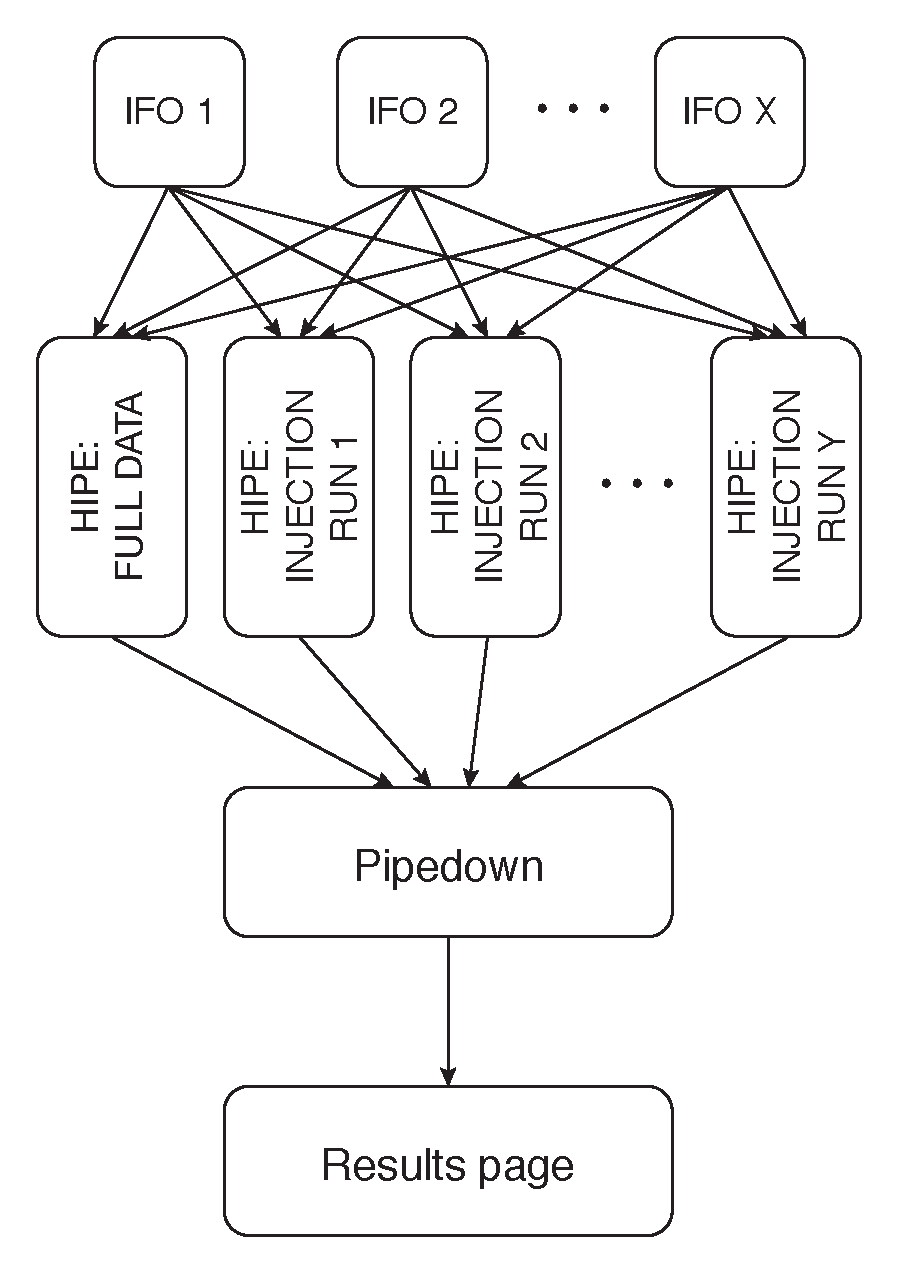
\includegraphics[width=2.5in]{figures/ihopeOverview.pdf}
\end{center}
\caption{
An overview of the \ihope pipeline. The HIPE and Pipedown nodes are themselves workflows, and are detailed in later sectionss.
}
\label{fig:ihopeOverview}
\end{figure}

\section{Pipeline Requirements}
\label{sec:PipelineRequirements}

Before delving into the details of \ihope, we briefly review the key
requirements of a pipeline used to search for \ac{GW}s. Our goal is to search
for \ac{GW}s from coalescing binaries in a range of masses. Hampering our
efforts is the fact that gravitational waves couple very weakly to matter; we
must be able to detect strains of $\sim10^{-21}$. Despite this, we
aim to detect at a \ac{SNR} of $8$ in each detector to ensure statistical
confidence in our search.

When averaged over time the detectors' have a colored-Gaussian noise
distrubtion; as shown in Chapter \ref{ch:pipeline_principles}, the best analysis tool to search for signals is therefore a
matched filter \cite{?}. Match filtering requires knowing the morphology of the
waveform. Fortunately, binaries with total masses (\mtotal) less than $25\Msun$
sweep through the \ac{LIGO} and Virgo bands during their {\it inspiral} phases.
This means that the waveform from these systems can be well modelled by the
post-Newtonian approximation. For higher-mass systems ($25 < \mtotal/\Msun <
100$), in which the merger and ringdown part of the waveform become important,
numerical relativity waveforms can be stiched to the \ac{pN} approximation;
phenomenological waveforms may also be used. Thus, to cover the desired range,
we can fill a bank of templates using the methods described in section \ref{sec:multiple_templates} of Chapter \ref{ch:pipeline_principles}.

Environmental and instrumental factors can cause non-Gaussian transient noise
(\emph{glitches}) in the data. To deal with this our pipeline must be able to
distinguish between triggers resulting from glitches and triggers resulting
from gravitational waves. Since the morhpology of the signals is known, the
$\chi^2$ test discussed in Chapter \ref{ch:pipeline_principles} lends itself as
a good method to do this. Checking for coincident triggers in multiple
detectors will also filter out spurious triggers since we do not expect
environmental correlations across great distances. After all filtering and
tests have been applied, the statistical significance of a set of triggers has
to be evaluated to determine the probability that a gravitational wave exists
in the data. A pipeline must therefore be able to compute a background with
which to compare triggers to. To avoid bias, this must be done in a {\it blind}
fashion: the method by which background is chosen and triggers ranked must be
chosen without knowledge of what is in the data, else the results will sway in
the favor of the analysts' bias. 

Finally, the pipeline must be able to evaluate its sensitivity and efficiency
to sources in the universe. Doing so allows tuning studies to be carried out
prior to doing the full analysis, and for the astrophysical rate of \ac{CBC}s
to be bounded after the analysis has completed. This can be done by performing
\emph{injections} of signals with known parameters into the detectors. Both \emph{hardware} and \emph{software} injections may be performed. Hardware injections
involve actuating the mirrors to physically simulate a passing gravitational
wave. This is the most robust test as it checks the ability of the detectors'
response loop to measure \ac{GW} strains and the ability of the pipeline to
detect them. The trouble with hardware injections is that real \ac{GW}s cannot
be detected while they are occurring, limiting the number that can be done.
Software injections involve adding a gravitational wave signal to the data
stream on disk just prior to analyzing it. While this method doesn't test the
hardware control systems, it has the advantage that it can be done many times
in parallel, without corrupting the original data. Thus, our pipeline must be
able to perform software injections, and have a method for associating triggers
with the injections that went into the data.

In summary, a pipeline used to search for gravitational waves from \ac{CBC}s must:
\begin{itemize}
\item{construct a bank of templates with which to filter;}
\item{identify \emph{triggers} by filtering templates through the detector data;}
\item{distinguish noise triggers from gravitational wave triggers;}
\item{quantify statistical significance of triggers and rank them in a blind manner;}
\item{evaluate the sensitivity and efficiency of the search to \ac{CBC}s in the universe.}
\end{itemize}
In the following sections we will see how \ihope meets these requirements.


\section{\ihope at Runtime}
\label{sec:ihopeRuntime}

The \ihope pipeline is created by running \texttt{lalapps\_ihope}. This sets up
the workflow by doing the following at run time:

\begin{itemize}
\item{set-up the directory structure to save all data to;}
\item{copy all needed programs from their installed location to a local directory;}
\item{retrieve analysis start and stop times;}
\item{download a {\it veto-definer file} and find the start and stop times of all veto segments;}
\item{run \texttt{lalapps\_inspiral\_hipe};}
\item{run \texttt{lalapps\_cbc\_pipedown};}
\item{create a cache file of the names and locations of all files that will be created;}
\item{write a DAX that can be used to start and run the worflow.}
\end{itemize}

These steps require the start and stop time (in GPS seconds) of the period to
be analyzed as well as a configuration file. The configuration file is a text
file containing all the information needed to setup and run the analysis. This
includes: the names and locations of all the executables that will be run;
variable arguments that these programs will need; the name and number of
interferometers to analyze; the version of data files to retrieve and what
channels to analyze; how many and what type of software injection runs to do;
any other information needed by the \ac{DAG}s to run. The configuration file
provides a convenient way to manipulate the pipeline. Changing tuning
parameters is largely accomplished by editing this file. Likewise, the
difference between running a {\it low-mass} search ($2 < \mtotal/\Msun < 25$)
and a {\it high-mass} search ($25 < \mtotal/\Msun < 100$) is determined
entirely by the configuration file.

A directory named by the gps start/stop times is created at runtime. All work
is done in this directory. In it, a \texttt{segments}, \texttt{executables},
\texttt{datafind}, \texttt{full\_data}, and \texttt{pipedown} directory are
created, along with a directory for each injection run that will be carried
out. With the exception of the \texttt{executables} and \texttt{segments}
directory, each of the sub directories store a sub-\ac{DAG} that will be run
during the analysis (and will be explained below). The master \ac{DAG} is saved
in the gps-times direcotory along with a master cache file of all the files
that will be created. All programs that will be run are copied to the
\texttt{executables} directory.

\subsection{Science and Veto Segments Retrieval}
\label{sec:science_segs_and_vetoes}

The \ac{LIGO} and Virgo detectors can be in one of five different states at any
given time. We are only interested in analyzing times in which the detectors
are in {\it Science} mode. This means they are up, locked, and no other
experimental work is being done on them \cite{?}. The interferometers
can drop out of Science mode many times across an analysis period; thus \ihope
must retrieve the start and stop times of Science segments that occurred in the
desired analysis period. \ihope does this by running
\texttt{ligolw\_segment\_query} at run time. This program queries the {\it
segment database} --- a remote database that contains lists of segments
detailing the times that each of the detectors were in various states --- to
retrieve the list of Science times during the desired analysis period. These
results are saved to xml files in the \texttt{segments} directory. These files
do not contain strain data; they only list the times that data can be
retrieved. The results are later used to retrieve files containing strain data.

Various environmental and instrumental factors can cause periods of elevated
glitch rate during Science mode. If these periods are analyzed with periods of
relatively clean data, they will pollute the background estimation, thereby
decreasing statistical confidence in candidates. We therefore seek to remove
such periods from the analysis. This is accomplished using vetoes. Vetoes are
categorized according to how well we can couple them to known environmental
sources; they are applied cumulatively. Table \ref{tab:vetocats} lists the
various categories and their defining characteristics. For \ac{CBC} searches,
we do not analyze anything prior to category 1; i.e., all matched filtering is
done after category 1 vetoes are applied. Category 2 and 3 vetoes are applied
when second stage coincidence is carried out (see HIPE, below). We quote false
alarm rates and base upper limits on data in which category 1-3 vetoes have
been applied. We additionally check the data after category 1 and 2 vetoes have
been applied for any loud triggers that may have been removed by category 3
vetoes. We do not use category 4 for the anlaysis; however, we do use them in
follow-up studies of loud events to provide insight into the cause of the
events. Hardware injections are left in the data after category 1 and 2, and
are removed as a special veto prior to category 3 vetoes being applied.

\begin{table}
\label{tab:veto_cats}
\center
\begin{tabular}{c | p{5cm} | p{8cm}}
Category    &    Description    &   Procedure    \\
\hline
    1       &    Data seriously compromised or missing.    &    Data never analyzed. \\
\hline
    2       &    Instrumental problems with known coupling to h(t).    &    Vetoed triggers discarded after second coincidence. Surviving triggers checked for candidates, but not used for upper limits. \\
\hline
    3       &    Instrumental problems likely, casting doubt on triggers found during these times.    &    Vetoed triggers discarded after second coincidence. False alarm rates of surviving triggers are used in publications; upper limits are calculated using these vetoes.  \\
\hline
    4       &    Positive, but weak, correlations with false alarms. Large dead times.    &     Not used in the analysis, but used as a guide in detailed followups of loud triggers. \\
\end{tabular}
\caption{The various veto categories used by the \ac{CBC} group. Vetoes are applied cumulatively; statistical significance of candidates and upper limits are calculated after category 1, 2, and 3 vetoes are applied.}
\end{table}

Vetoes are triggered by environmental and instrumental channels that flag
various segments of time for suspicious activity. Additional flags can be added
by hand; e.g., if a truck drives onto the site during Science mode, a person
in the control room may add a flag for that period of time. All of these flags
are stored in the segment database. What flags to use for vetoes, at what
category, and for how long, are stored in a \emph{veto-definer file}. This xml
file contains a \texttt{veto\_definer} table that lists each flag that should
be used, what category the flag should be used at, the dates the flag is valid, and any
padding (in seconds) to add to the flag should it go off. Entries are added to
this table by hand after extensive data-quality investigations and safety
checks. Vetoes are fine tuned for specific searches and epochs, and each
searches' set is saved in a different veto-definer file in a central
repository. What veto definer file to use is specified in the \ihope
configuration file. At run-time, \ihope downloads the desired file to the
\texttt{segments} directory. It then runs \texttt{ligolw\_segments\_from\_cats}
to query the segment database for flags specified in the veto-definer file. The
vetoed segments for all of the instruments are added together and saved in xml
files in the \texttt{segments} directory.


\subsection{HIPE}
\label{sec:hipe_overview}

Once the analyzable Science segments and the veto segments that will be applied
are obtained, \ihope runs \texttt{lalapps\_inspiral\_hipe}. This sets up the
\ac{HIPE}, which is the pipeline that carries out the search. Figure
\ref{fig:HIPEDiagram} shows the \ac{HIPE} \ac{DAG} for a single $2048\rm{s}$
block of time. As can be seen in the diagram, \ac{HIPE} is a \emph{two-stage}
pipeline. Data is matched-filtered, coincidence tests are applied, then the
process is repeated. The reason for using two-stages is the $\chi^2$ test is
computationally expensive. Therefore, to cut down on the number of triggers for
which we need to compute $\chi^2$, an initial coincidence test is
applied.\footnote{Using two stages complicates the pipeline, however, and makes
it difficult to trace an event's progression through the various steps. It also
hampers efforts to estimate \acp{FAR} from single-\ac{IFO} triggers. For this
reason, a single-stage pipeline is being worked which takes advantage of
advances in computational power. See Chapter \ref{ch:future_developments} for
more details.}

\ac{HIPE} can be run both with and without injections. If injections are
desired, \texttt{lalapps\_inspinj} is run to create a list of injections to
make, which are created and inserted into the data just prior to match
filtering by \texttt{lalapps\_inspiral}. In order to create data with and
without injections, \ihope runs \ac{HIPE} several times: once for zero-lag and
time-slid data (which we label \texttt{FULL\_DATA}), and once for each desired
injection run, which are specified in the configuration file.

As discussed in section \ref{sec:pipeline_requirements}, we must be able to
estimate a background and calculate triggers in a blind fashion. However, we
must also be able to tune the pipeline so as to improve the chances of
detecting something. To satisfy these conflicting requirements, we have
designated a subset of data as \emph{playground}. Playground is defined as data
that occurs during the first $600$ seconds of every $6370\th$-second block of
time, starting from February 14, 2003 at 16:00:00 UTC (GPS time $729273613$).
It therefore consists of $\sim10\%$ of the full data. Playground is looked at
prior to un-blinding the rest of the data (what we colliquoly call
\emph{opening the box}) in order to tune vetoes and check for any spurious
results that would indicate a bug in the analysis. Although playground is
included in the final open-box analysis, we exculde it for computing
upper-limits. It is possible to run \ac{HIPE} such that it only analyzes
playground data; however, it is unnecessary, as we can easily retrieve
playground triggers from the \texttt{FULL\_DATA} analysis using their
end-times. Details of \ac{HIPE} are discussed in section \ref{sec:HIPEdetail}.

\begin{figure}[p]
\begin{center}
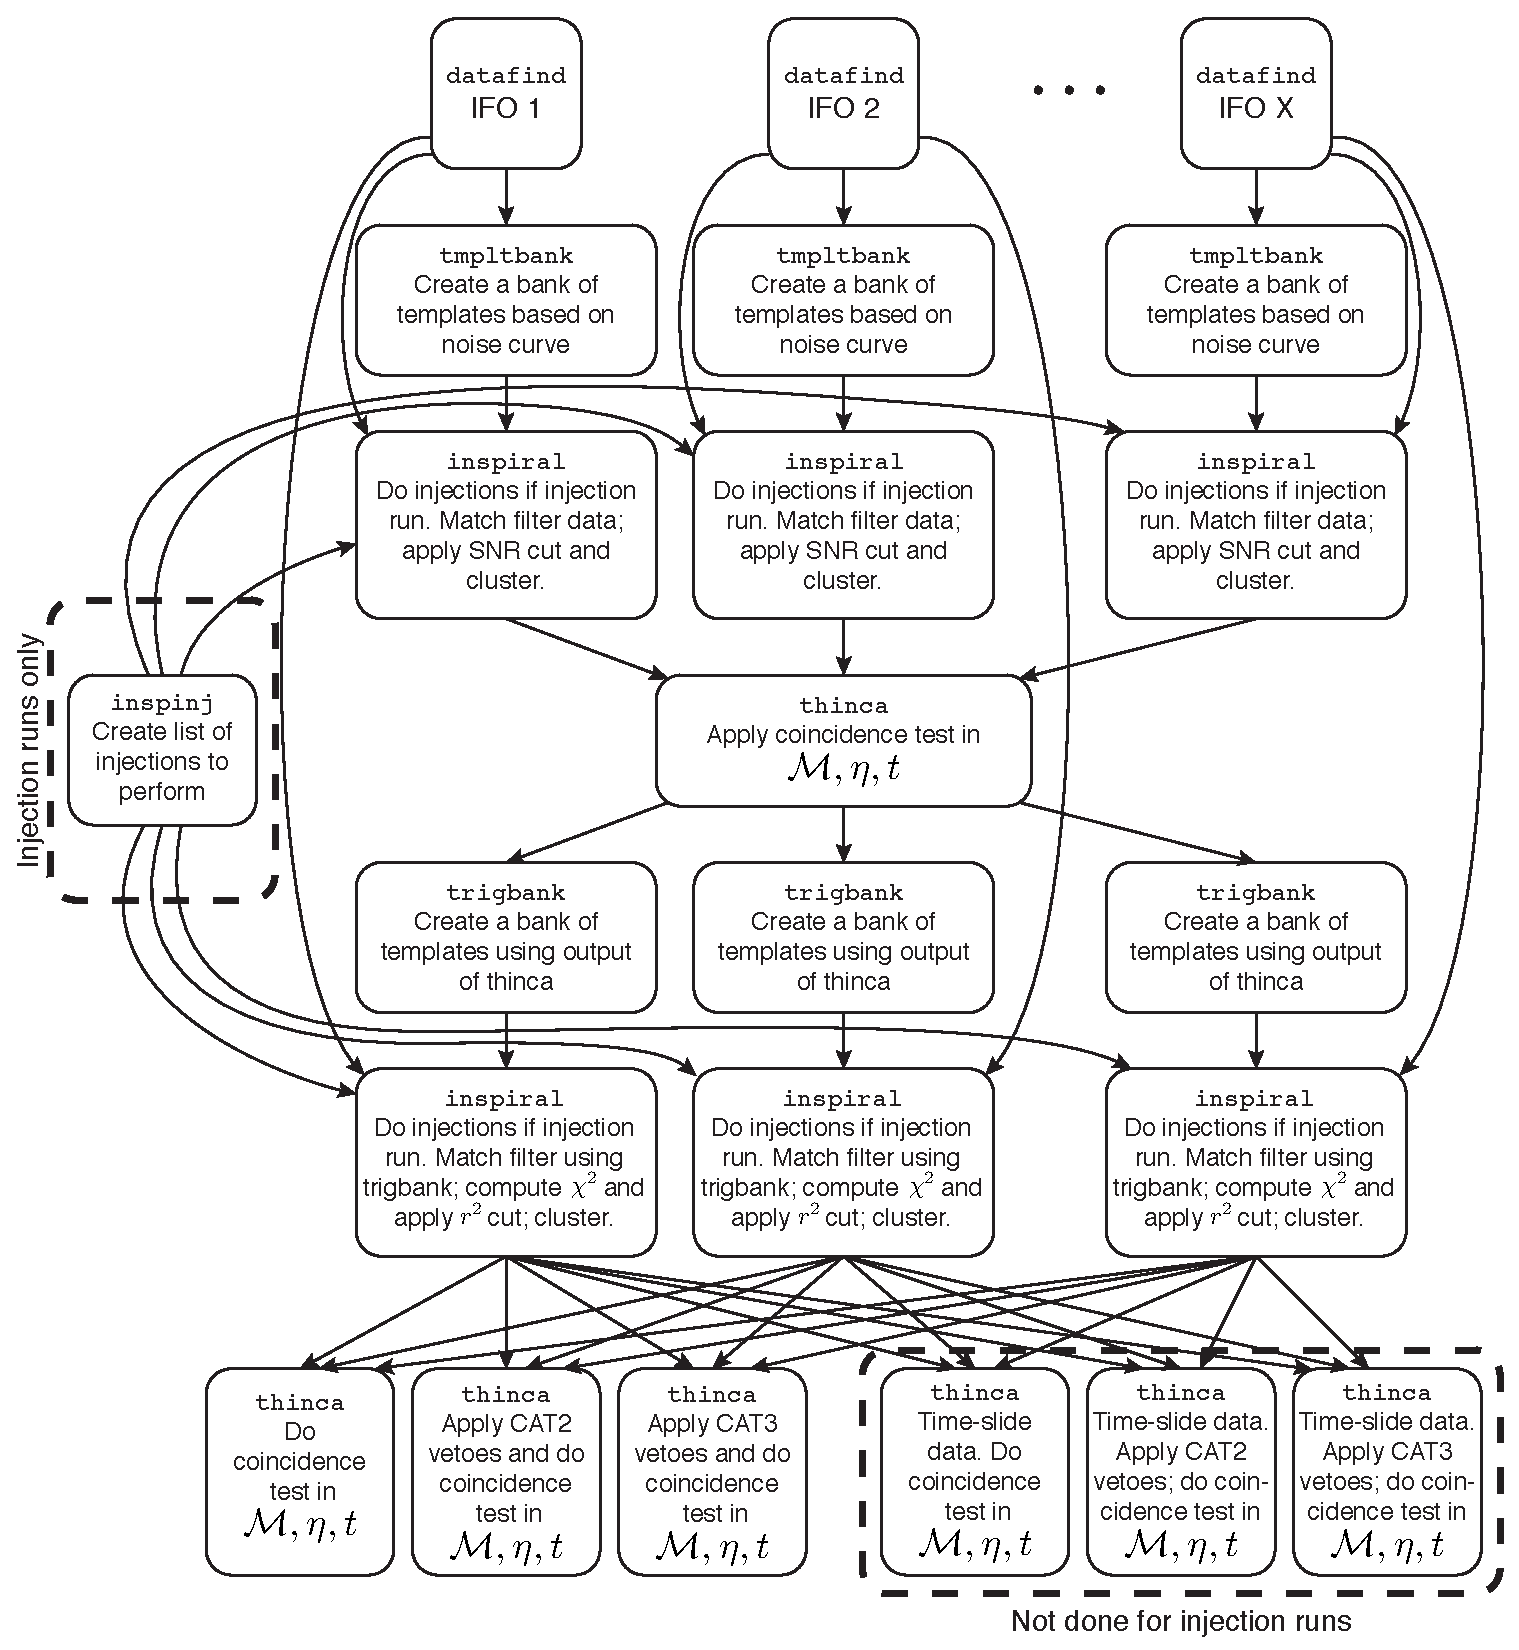
\includegraphics[width=6in]{figures/HIPEDiagram.pdf}
\end{center}
\caption{
The \ac{HIPE} pipeline. This is run once for full-data and once for
each injection run. For injection runs, \texttt{lalapps\_inspinj} is run to
generate a list of injections to create, and time slides are not done.
}
\label{fig:HIPEDiagram}
\end{figure}

\subsection{Pipedown}
\label{sec:pipedown_overview}

After all the instances of \texttt{lalapps\_inspiral\_hipe} have run, \ihope
run \texttt{lalapps\_cbc\_pipedown} which sets up the Pipedown \ac{DAG}.
Pipedown takes the results of all the different HIPE runs, combines them into
SQLite databases, computes and ranks triggers by \ac{FAR}, and creates plots
and tables of the results. Figure \ref{fig:PipedownDiagram} details the steps
Pipedown takes to carry out these goals. Shown are the steps taken for a single
veto-category; this diagram is repated for each veto-category (by Pipedown, not
by \ihope). In-depth details of Pipedown are discussed in Section
\ref{sec:PipedownDetail}.

\begin{figure}[p]
\begin{center}
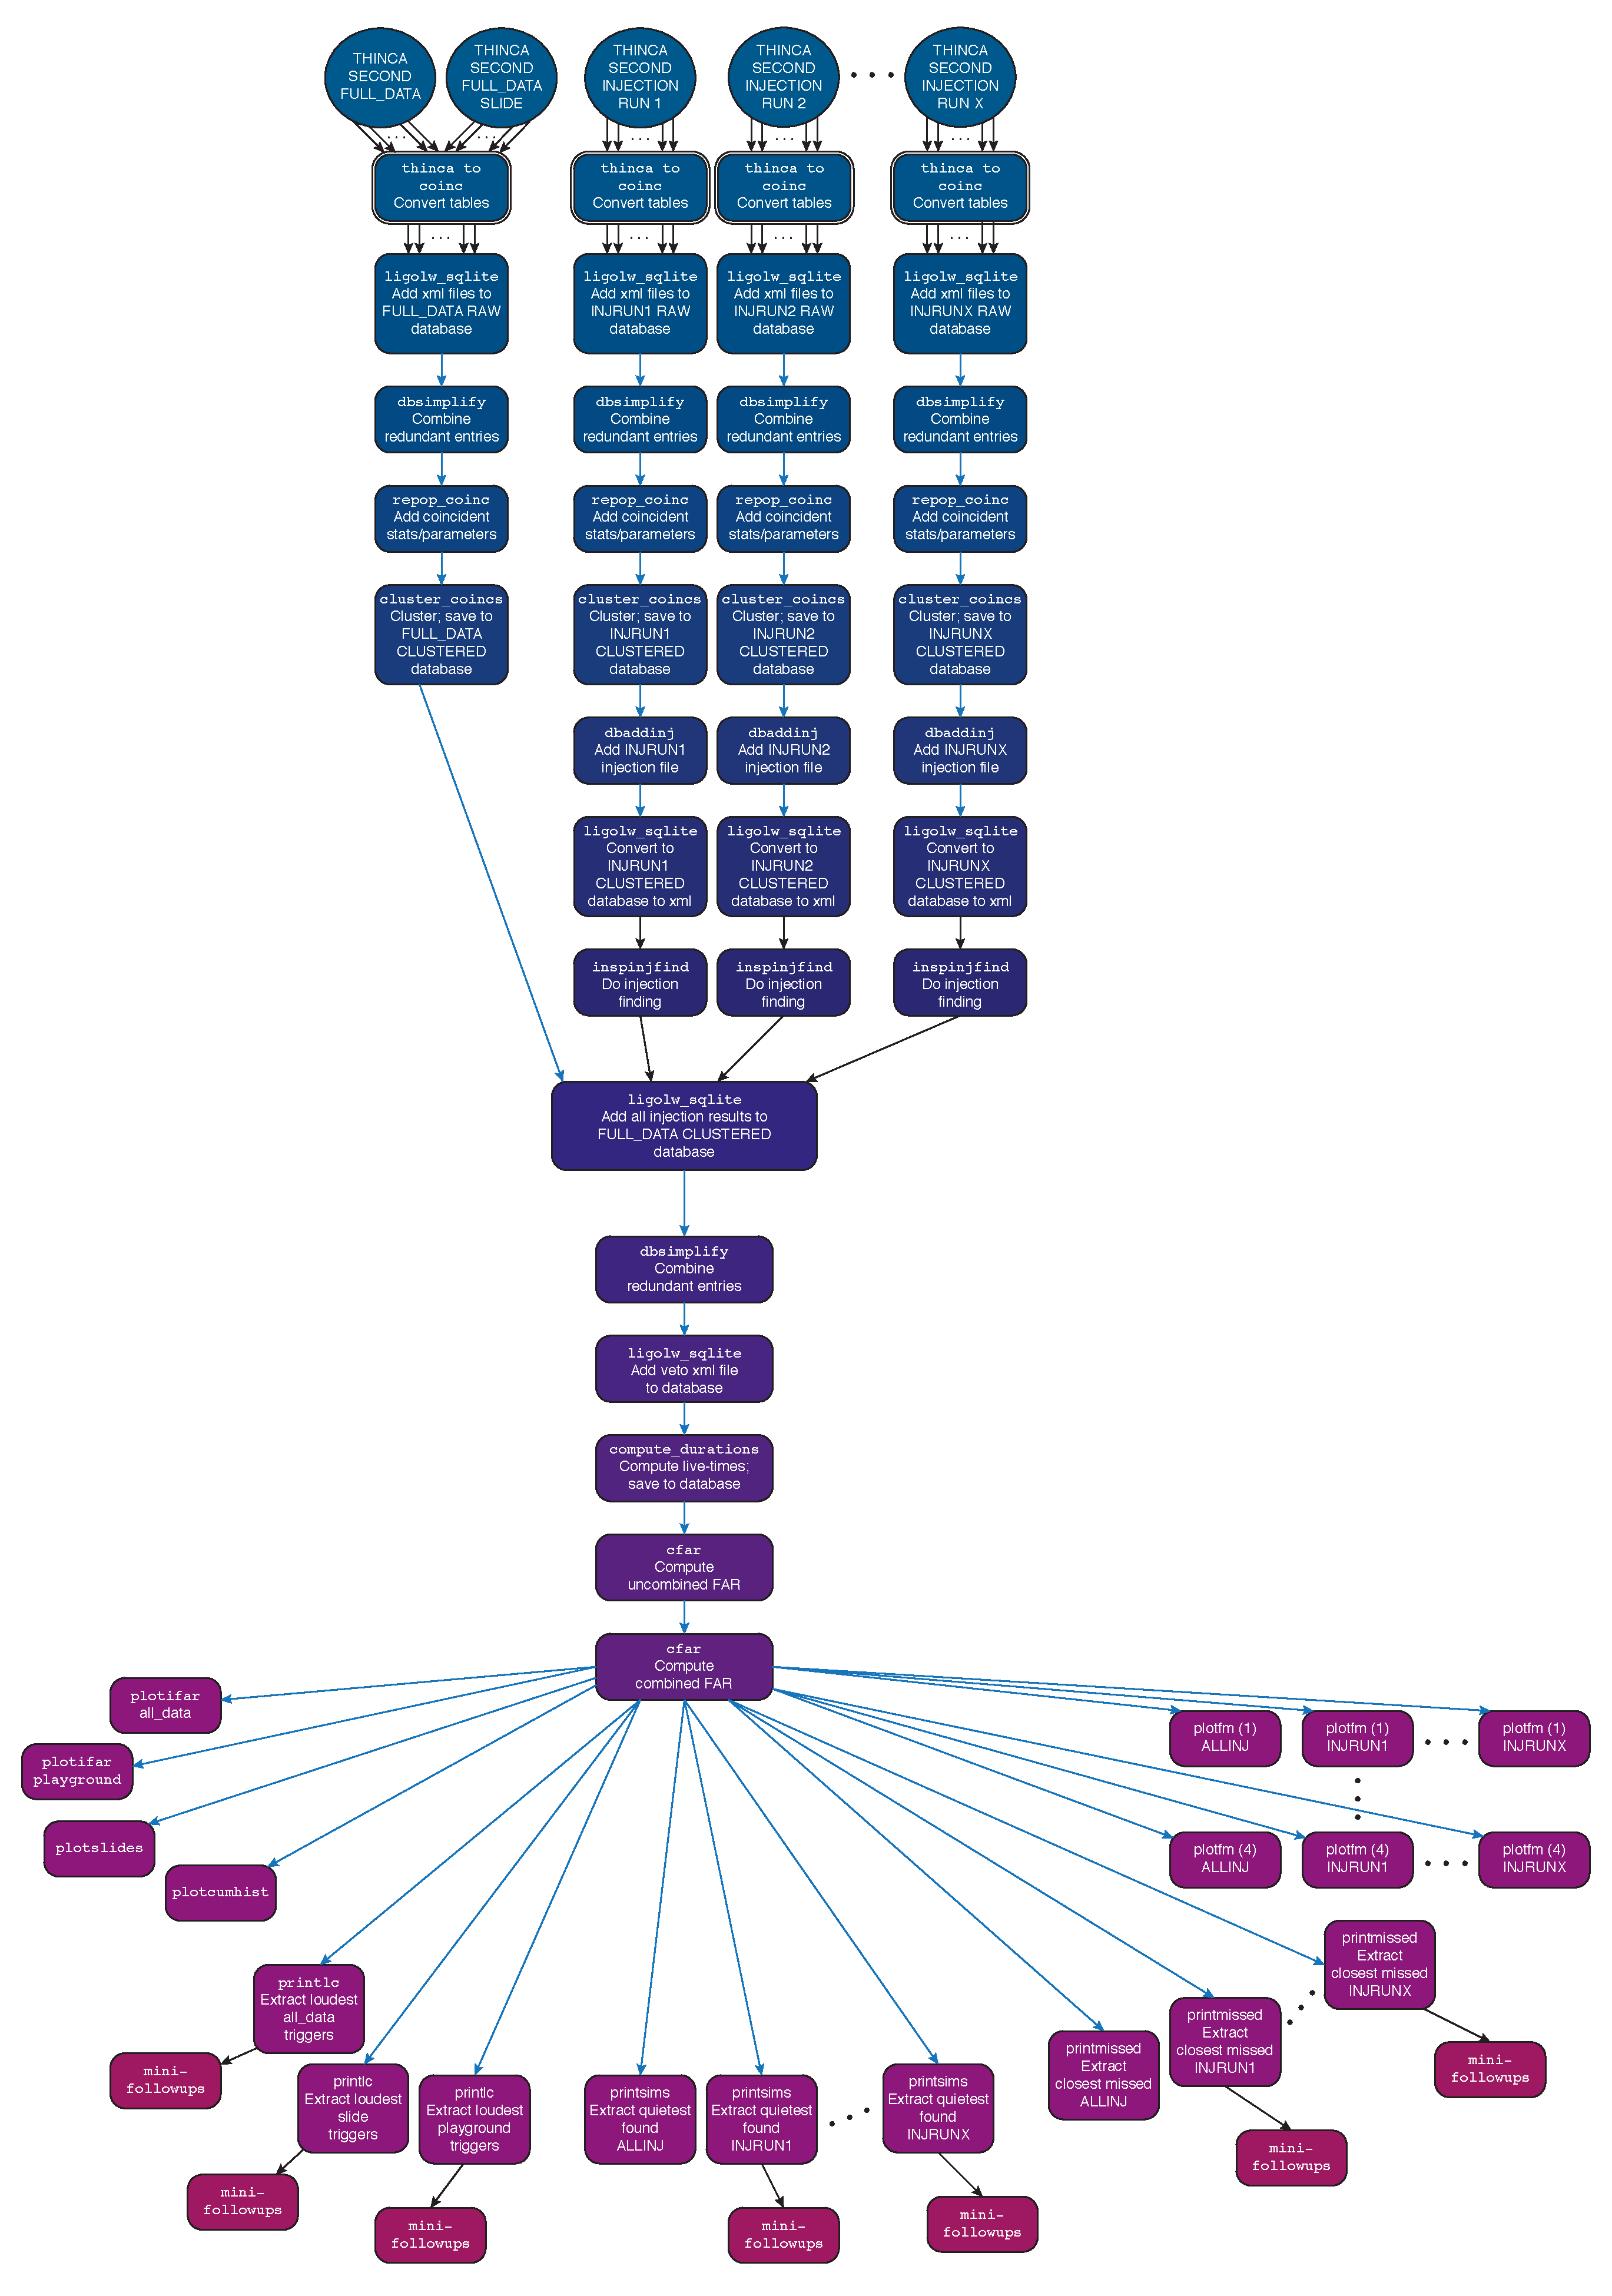
\includegraphics[width=6in]{figures/PipedownDiagram.pdf}
\end{center}
\caption{
The Pipedown pipeline for a single veto category. Each block represents a single node. Double bordered blocks represent multiple nodes. Circles represent batches of files. Black arrows represent xml files; blue arrows, SQLite databases. Each arrow represents a single file.
}
\label{fig:PipedownDiagram}
\end{figure}

\subsection{DAX}
\label{sec:DAX}

After pipedown has completed, \ihope writes a DAX that can be used to launch the pipeline. A DAX is an abstract workflow in which elements such as file locations are variables. The DAX is turned into a \ac{DAG} by the Pegasus Workflow Management Service.

\section{HIPE in Detail}
\label{sec:HIPEdetail}

We now step through \ihope in detail, using a toy analysis of $10,240$s as an example. In this analysis we will use three interferometers: the 4-kilometer Hanford detector (H1), the 4-kilometer Livingston detector (L1), and the 3-kilometer Virgo detector (V1), and we will add one injection run, which we label \texttt{BNSINJ}. Figure \ref{fig:science-selected_segs} shows the segments that are available to analyze during this time. The \emph{selected segments} are Science segments minus CAT1 veto segments; they are what \ihope passes to \ac{HIPE} to analyze.

\subsection{Data Find}
\label{sec:data_find}

As can be seen in Figure \ref{fig:HIPEDiagram}, the first step in \ac{HIPE} is to run \texttt{lalapps\_data\_find}. Data from all of the interferometers are stored in \emph{frame files} in central locations at every computer cluster. Frame files can contain multiple channels recorded from the interferometers. For analysis purposes, we are only interested in files containing the strain data channel, which is called \texttt{LDAS-STRAIN} in the \ac{LIGO} detectors and \texttt{h\_16384Hz} in Virgo. \texttt{lalapps\_data\_find} finds the files covering the selected segments on the cluster and creates cache files listing the location of each these files in the \texttt{datafind} directory. These cache files are passed to \texttt{lalapps\_tmpltbank} and \texttt{lalapps\_inspiral}, which use them to locate and open the frame files for analysis.

\subsection{From Continuous to Discreet Data}
\label{sec:cont_to_discreet}

So far, all equations we have used involving Fourier Transforms and the inner product have assumed continuous time- and frequency-domain data series. Likewise, the integrals over frequency space have been from $-\infty$ to $+\infty$. In practice, of course, the data is discreetly sampled and is neither continuous nor infinite. Both the \ac{LIGO} and Virgo strain data are sampled at $16384\,\mathrm{Hz}$. Since even the lowest mass templates (i.e., waveforms with the highest frequency components) used in current \ac{CBC} searches terminate at frequencies around a couple of kHz, this sampling rate is much higher than is needed for our purposes. To ease computational requirements the time series is therefore downsampled to $4096\,\mathrm{Hz}$ prior to analysis. This sampling rate sets the Nyquist frequency, $f_{\mathrm{Nyquist}}$, at $2048\,\mathrm{Hz}$. To prevent aliasing, a low-pass time-domain digital filter with a cutoff at $f_{\mathrm{Nyquist}}$ is implemented to pre-condition the data. On the low-frequency end, seismic noise dominates the interferometers' power spectrum. We therefore also impose a high-pass digital filter in the time domain. The cutoff frequency of the high-pass filter, $f_c$, is set to be a several Hz lower than a low-frequency cutoff, $f_0$, that is determined by the characteristics of each \ac{IFO}'s power spectrum. These values are set in the configuration file. (For the values chosen for \ac{S5} and \ac{S6} see Chapters \ref{ch:s5_results} and \ref{ch:s6_results}, respectively.) Both the low and high-pass filters will ring at the start and end of a time series, corrupting the data. Thus we must remove the first and last $t_{\mathrm{pad}}$ of data after applying the filters and prior to analyzing. The duration of $t_{\mathrm{pad}}$ is also set in the configuration file; for both \ac{S5} and \ac{S6} we used $8\,$s.

To Fourier Transform the data, we use the \ac{FFT} algorithm. The \ac{FFT} imposes two constraints on the data. First, the number of points in the data series must be a power of two. Second, the \ac{FFT} associates the last point of the data series with the first point; i.e., it wraps the data around on a loop. This means that as a template is slid toward the end of the time series, any points extending beyond the end of the series will be placed at the beginning. Additionally, because the last and first point of the time series are discontinuous, the wrap around essentially introduces a delta function at the end of the series. As the template passes past the discontinuity it will ring (i.e., the match filter will return the template's impulse response), and, due to the wrap around, this ringing will be placed at the beginning of the time series. Thus the first $t_{\mathrm{chirp}}$ points of the \ac{SNR} time series are corrupted, where $t_{\mathrm{chirp}}$ is the \emph{chirp length} of the template, and must be thrown out.

The chirp length is defined as the length of time it takes for the binary to go from $f_0$ to the frequency at which the binary passes \ac{ISCO}, $f_{\mathrm{isco}}$. \ac{ISCO} is the point when the separation distance is too small for the binary's masses to maintain stable orbits without external energy being added to the system; at this point the masses cease to inspiral and plunge into each other.\footnote{Note that \ac{ISCO} is not the same as the Schwarzschild radius; e.g., in a Schwarzschild space-time, \ac{ISCO} occurs at $r = 6GM/c^2$ whereas the Schwarzschild radius occurs as $r = 2GM/c^2$.} Since the \ac{pN} approximation breaks down at $f_{\mathrm{isco}}$, we must terminate all integrals at this point. Combining this with the realities of Nyquist and seismic noise, all frequency domain integrals are limited to the region $f \in [f_0, f_{\mathrm{max}})$ where $f_{\mathrm{max}} = \min(f_{\mathrm{Nyquist}},~f_{\mathrm{isco}})$.

The \ac{PSD} is estimated using Welch's method. This involves breaking a data segment up into several bins of equal duration. Within each bin, the data is transformed to the frequency domain via the \ac{FFT}. Thus the number of points in each bin must be a power of two, and the bins must be overlapping to account for the wrap-around corruption at the beginning and end of each segment. Since the data is discreet, this results in a discreet number of frequency bins. The \emph{median} value within each frequency bin is then chosen across all the data segments to construct $S_n(|f|)$. We use the medain --- as opposed to the mean --- to better buffer the \ac{PSD} from over-estimation in the prescence of a signal.

As was the case with the template, $S_n(|f|)$ will be corrupted by the discontinuity between the first and last point of the data series. However, unlike the template, which has a finite duration, $S_n(|f|)$ will ring for the entire data segment. This ringing will also happen if a delta-function like glitch exists in the data. To prevent the entire segment from being corrupted, we \emph{truncate} the \ac{PSD}. This is done by estimating \ac{PSD} using Welch's method, inverse transforming $\sqrt{S_n^{-1}(|f|)}$ to the time domain, zeroing out the first and last $t_{\mathrm{invspectrunc}}$ seconds of the time series, then transforming back to the frequency domain. This limits the corruption due to the wraparound to the first and last $t_{\mathrm{invspectrunc}}$ seconds of the time series. The truncation does cause some smoothing out of high Q features, such as power-line harmonics; however, since we search for relatively broad band signals this smoothing has little effect on the search. The value of $t_{\mathrm{invspectrunc}}$ was set to $8\,$s for both \ac{S5} and \ac{S6}.

For more details on \ac{PSD} estimation and implementation of the matched filter with a discreet and finite time-series, see \cite{ref:Brown} and \cite{ref:FindChirp}.

\subsection{Data Segmentation}
\label{sec:data_segmentation}

\texttt{lalapps\_inspiral} is the program that constructs the \ac{SNR} time series for templates laid out in a bank by the program \texttt{lalapps\_tmpltbank}. The \ac{SNR} time series is constructed according to equation \ref{eqn:snr_full_form} and the templates are laid out using the metric defined in equation \ref{eqn:templateMetric}. Since both of these equations involve the inner product defined in equation \ref{eqn:inner_product}, both programs must compute the \ac{PSD}, $S_n(|f|)$, as well as the Fourier Transform of the data, $\widetilde{s}(f)$. (We do not Fourier Transform the templates. Instead, we generate the templates in the frequency domain directly by using the \ac{SPA}.)

The wrap around of the \ac{FFT} and the Welch median \ac{PSD} estimation method put limitations on how much data can be analyzed at once; they also require data to be overlapped due to corruption at the start and end of segments. These considerations require us to carefully segment the data for analysis. The things we must consider are:
\begin{itemize}
\item{The low-pass and high-pass digital filters corrupt the first $8\,$s of an analysis segment, or \emph{chunk}.}
\item{In order to estimate the \ac{PSD} using the Welch median method, we must break the chunk up into several segments; data in each segment is transformed via the \ac{FFT} independently.}
\item{The \ac{FFT} requires the number of points in each segment to be a power of two.}
\item{The wrap around of the \ac{FFT} causes the first $t_{\mathrm{chirp}}$ seconds of each segment to be corrupted due to the template, and the first and last $8\,$s of the segment to be corrupted due to the inverse \ac{PSD}.}
\item{Each segment must therefore overlap so as not to lose data from the corrupted parts of the \ac{FFT}.}
\end{itemize}
In initial \ac{LIGO} the low-frequency cutoff $f_0$ was set to $40\,$Hz. In the low-mass \ac{CBC} search, the longest template is therefore $\sim33\,$s in duration. The smallest power of two larger than $33$ is $64$; thus the first $64\,$s of each segment must be overlapped by a previous segment. The end of each segment only needs to be overlapped by $8\,$s to account for the \ac{PSD} corruption. However, for book-keeping simplicity, we chose to also discard the last $64\,$s of each segment. Thus, all the segments must overlap each other by $128\,$s. Since the segments must be a power of two, this means each segment must be $256\,$s in duration.

In deciding upon the number of segments to use in the median \ac{PSD} estimate we must consider a few factors. The more segments we have, the more accurate the \ac{PSD} estimation will be. However, more segments also means that more time will be grouped together. If the \ac{PSD} changes over this period, our estimate will be off. Furthermore, the number of segments used sets a minimum period of time that we must have continuous data. If a selected segment is shorter than that period, we cannot analyze it. 

In inital \ac{LIGO} we have chosen to use 15 overlapping segments for each \ac{PSD} estimation. Since each segment is $256\,$s long, with overlaps of $128\,$s, this means that each chunk must be $2048\,$s long. Add to this the needed $8\,$s pad at the start and end of the chunk to account for the corruption of the filters, and we find that we need a continous $2064\,$s of data in order to do the analysis. If a selected segment is longer than $2064\,$s, then it will be broken up into several chunks. Each chunk is overlapped by $72\,$s to account for the time thrown out at the beginning/end of the first/last segment in each chunk and the $8\,$s pad. If the selected segment is not a multiple of $2048$ (as it most likely will not be), then the last chunk in the segment is overlapped more so as to analyze the entire period. The segments in this last chunk that overlap with non-corrupted time in the previous chunk are simply not match filtered, although they are used for the \ac{PSD} estimation of the last chunk.

The effects of this data segmentation on our toy analysis can be seen in Figure \ref{fig:segment_plot_full}. The top three lines show the selected segments. Each \texttt{TMPLTBANK} and \texttt{INSPIRAL} jobs corresponds to a single chunk in a single \ac{IFO}. As can be seen, every chunk overlaps by $72\,s$, except for the last one in each segment. Also note the first selected segment in V1. As seen in Figure \ref{fig:science-selected_segs}, a CAT 1 veto broke the V1 Science segment into two selected segments. Since the first selected segment is only $\sim900\,$s long, it cannot be analyzed. This can be seen in the \texttt{TMPLTBANK} and \texttt{INSPIRAL} lines: there are no V1 jobs covering this period. This is part of the reason why CAT 1 vetoes are only used for seriously compromised data. Overuse of CAT 1 vetoes could lead to large amounts of unanalyzed time if they broke the data up into selected segments that were shorter than $2064\,$s.

\subsection{Template Bank}
\label{sec:tmpltbank}

The first step in the \ac{HIPE} pipeline after data find is to create a template bank. As stated above, \texttt{lalapps\_tmpltbank} is the program that constructs the bank. \ac{HIPE} creates one \texttt{tmpltbank} job for each \ac{IFO} and for each chunk. Since the \ac{PSD} is re-estimated for each chunk the metric will change from job-to-job, resulting in a different template bank for each chunk and for each \ac{IFO}. However, the changes in the \ac{PSD} are usually small, and so the bank stays roughly the same across an analysis period. In order to calculate the \ac{PSD} \texttt{lalapps\_tmpltbank} reads in the frame cache, loads the data, applies the low- and high-pass filters, downsamples to $4096\,$Hz, then computes the \ac{PSD} using the Welch median method.

Variables such as what \ac{pN} order to use to lay out templates, what space to lay them out in, and what minimal match to use are command-line arguments to \texttt{lalapps\_tmpltbank} and can therefore be set in the configureation file. As stated in Chapter \ref{ch:pipeline_principles}, for \ac{S5} and \ac{S6} the bank was laid out in $\tau_0$ and $\tau_3$ space using $2.0$ restircted \ac{pN} templates to calculate the metric, with a minimal match $\geq 97\%$. The \ac{pN} order of the templates themselves do not have to be the same as the order used to compute the metric. Indeed, while $2\,$\ac{pN} templates were used for \ac{S5}, for \ac{S6} restricted $3.5\,$\ac{pN} templates were used. Since the metric and best coordinates to use is currently unknown for $3.5\,$\ac{pN} templates, we had to use the $2\,$\ac{pN} metric. Investigations are underway into obtaining the $3.5\,$\ac{pN} metric.

Figure \ref{fig:template_bank} shows a typical template bank in both $\tau_0,~\tau_3$ space and in $m_1,m_2$ space for the low-mass \ac{CBC} search.\footnote{Note that the maximum total mass in these plots extends to $35\,\Msun$. This was reduced to $25\,\Msun$ for the last part of \ac{S6}. See Chapter \ref{ch:s6_results} for details.} The parameters of each of these templates are stored in a \texttt{sngl\_inspiral} table (see section \ref{sec:data_storage} for details), which is saved in an xml file. Also stored in the \texttt{sngl\_inspiral} table are the metric components around each template. Each \texttt{tmpltbank} job outputs one xml file, with naming convention:
\begin{center}
\texttt{\{IFO\}-TMPLTBANK-\{GPS-START\}-\{DURATION\}.xml}
\end{center}
All of the \texttt{tmpltbank} files created in our toy $10240\,$s analysis can be seen in Figure \ref{fig:segment_plot_full}.

\subsection{Injections}
\label{sec:inspinj}

Software injections are the \ac{CBC} group's way to check that our pipeline is working.\footnote{As mentioned in section \ref{sec:PipelineRequirements} hardware injections exist too. These are also used to check that the pipeline is working. However, because we cannot perform the large number of hardware injections needed for Monte Carlo simulations --- as we can with software injections --- they are of limited use for tuning and efficiency studies.} Since the number we can perform is only limited by computational power, we can do a large number across a broad range of parameters and sky positions. Being able to do such Monte Carlo simulations allows us to test the efficiency of our pipeline, tune parameters, and calculate rate limits to compare to astrophysical expected rates.

Injections are only performed in injection \ac{HIPE} runs; these are later combined with non-injection runs by Pipedown. For example, in our toy analysis, we have chosen to do one injection run, which we labeled \texttt{BNSINJ}. If we are on an injection run then, prior to launching first inspiral jobs, \ac{HIPE} runs \texttt{lalappps\_inspinj}. \texttt{Inspinj} generates a list of injections to perform based on the input arguments. It does not create the waveforms themselves; that is left to \texttt{lalapps\_inspiral} (see below).

How the injections are distributed in mass, mass-ratio, sky-location, orientation, and time is determined by the configuration file. For a given injection run, a minimum and maximum component mass are specified, along with a maximum total mass. Additionaly, what mass parameter to distribute the injections in must be specified. For \ac{S5} and \ac{S6} injections were chosen to be distributed uniformly in component mass. How to distribute the location of injections is also required. In \ac{S5} a galaxy catalogue was used for the location distribution; random galaxies were chosen for an injection to occur in. For \ac{S6}, the range of the detectors was large enough to ignore inhomogenities in the universe; thus in \ac{S6} the location distribution was changed to be randomly distributed across the sky. The orientation of injections was distributed uniformly across inclination angles for both \ac{S5} and \ac{S6}.

Injections are distributed randomly in time. However, to prevent too many injections from occuring in the same period, a time-step and time-interval argument are added. The time-step argument sets the average period of time between each injeciton, and the time-interval sets the interval around that time-step in which an injection is randomly placed. For example, in \ac{S6} the time-step was set to $837\,$s and the time-interval was set to $300\,$s. This means that if an injection occurs at time $t_0$, the next injection will be chosen to randomly occur in the interval $(t_0 + 837) \pm 300\,$s.

We distribute injections in distance based on the range of the detectors. We are most interested in the region around the network's horizon distance, as this is where the efficiency quickly drops from $\sim1$ to $0$ (for a given false alarm rate). Since the detectors' sensitivity is mass dependent, we adjust the domain of distances in which to distribute injections according to the mass-range and type of injections being performed. Injections may be distributed uniformly in distance or in log distance. When we distribute uniformly in distance, we tend to over populate the outer regions of the range, since volume grows as $r^3$. If we distribute uniformly in log distance, we tend to over populate the inner regions of the range. For this reason, two injection sets are typically done for a single mass-range and injection type: one that is distributed linearly in distance and one distributed uniformly in log distance. Prior to analysis, the choice of injection ranges is based on a best-guess of what the range will be from \ac{PSD} estimations. Since we cannot know what the actual range of the network of detectors is until after the analysis is complete, extra injection runs are done after the analysis. These runs are set up to better target the range around the horizon distance so as to have good statistics for upper-limit calculations.

The waveform generator used by \texttt{lalapps\_inspiral} --- called \texttt{FindChirpSP} --- has the ability to create waveforms from several different template families, not just restricted non-spinning \ac{pN} templates. Thus we check how well spinning waveforms are recovered using our non-spinning template bank. This was done for both \ac{S5} and \ac{S6} searches, as separate upper-limits were produced for spinning \ac{NSBH} and \ac{BBH} systems. Additionally, we can check how well various waveform families overlap with the \ac{pN} approximation we use for the templates in the template bank. For example, in the \ac{S6} low-mass \ac{CBC} search, \ac{NSBH} injections were generated using the EOBNR psuedo-4\ac{pN} model.

Each injection \ac{HIPE} run will only draw from a single waveform family, with a give range of parameters, and with a given random-number-generator seed. To create a large number of injections, multiple injection runs are done; some of these will have the same range of parameter, with only the random seed changing. When \texttt{lalapps\_inspinj} runs in a given injection run, it saves the list of injections to perform to a \texttt{sim\_inspiral} table that lists the times, parameters, and waveform family of the injections to create. This table is saved to an xml file with naming convention:
\begin{center}
\texttt{HL-INJECTIONS\_\{SEED\}\_\{USER-TAG\}-\{GPS-START\}-\{DURATION\}.xml}\footnote{The \texttt{HL} prefix on the \texttt{INJECTIONS} file is an anachronism from when searches were only done between the two \ac{LIGO} sites. The \texttt{sim\_inspiral} table actually contains injection information for all the detectors in the search.}
\end{center}
\texttt{SEED} is the random seed given to \texttt{inspinj} in the given run. The \texttt{USER-TAG} is a unique identifier given to each \ac{HIPE} run by \ihope. The non-injection run will be named \texttt{FULL\_DATA} whereas each injection run will have a unique name to distinguish it from the other injection runs. Unlike the \texttt{FULL\_DATA} tag, the injections' \texttt{USER-TAG}s are set in the configuration file. For example, since we have done one injection run in our toy analysis, we have two unique user-tags: \texttt{FULL\_DATA} and \texttt{BNSINJ}. One \texttt{INJECTIONS} file exists for each injection run; this file is loaded by \texttt{lalapps\_inspiral} to insert the injections into the data.


\subsection{First Inspiral}
\label{sec:first_inspiral}

With the template bank and (for injection runs) list of injections generated, \ac{HIPE} next runs \texttt{lalapps\_inspiral} to match filter the data. One inspiral job exists for each \texttt{tmpltbank} job; i.e., there is an inspiral job for each \ac{IFO} and for each analysis chunk. Inspiral loads the frame cache and the template bank corresponding to its chunk. Additionally, if \ac{HIPE} is analyzing an injection run, it will read in an \texttt{INJECTIONS} file.

Inspiral carries out the same data conditioning as \texttt{tmpltbank} (in fact, they call the same code): data is read in, low- and high-pass filtered, and resampled. If \texttt{inspiral} is given an injections file it will create the waveforms that overlap its analysis time prior to data conditioning. Waveforms are generated in the time-domain using the parameters stored in the \texttt{sim\_inspiral} table and added directly to the data stream in memory. The data is then low- and high-pass filtered and resampled. Note that \texttt{tmpltbank} does not load injections. Instead, the same bank is used for both non-injection and injection runs. While this introduces a subtle difference from the real situaton, the effect on the template bank is negligible since the median estimator is used and since the number of injections in a chunk is limited by the time-step and time-interval arguments given to \texttt{lalapps\_inspinj}.

After the data is conditioned and the \ac{PSD} estimated, \texttt{inspiral} reads in a template from the \texttt{TMPLTBANK} file, generates it (in the frequency domain), then match filters it with the data to create the (complex) \ac{SNR} time series for the given template. This is repeated for each template in the bank file. For injection runs, an optional argument \texttt{enable-inj-filter-only} can be turned out that causes the \texttt{inspiral} to only filter segments containing an injection. This cuts down on computational time and has no effect on the analysis, since we are only interested in times around an injection (all other times are assumed to return the same result as the non-injection run).

As discussed in Chapter \ref{ch:pipeline_principles} we identify triggers by finding points where the \ac{SNR} ($\rho$) is at a maximum. Due to noise, however, there will be multiple local maxima across the duration of a template. We must therefore employ time-domain clustering on the \ac{SNR} so as to associate a single trigger with an event. This is done by using the \emph{max over chirp length} algorithm. Max over chirp length uses a sliding time window to select triggers: for every point in time, a point is only kept if there is no other point with a $\rho$ greater than it within the chirp length of the template. Once a trigger is identified, the time at which it occurs is associated with the \emph{coalescence}, or \emph{end-time}, $t_c$, of the binary. If the \ac{SNR} of the trigger exceeds our desired \ac{SNR} threshold, it is kept. The \ac{SNR} threshold is set in the configuration file; for both \ac{S5} and \ac{S6} it was set to 5.5.

Due to the high overlap between templates in the bank, a single event can create triggers across multiple templates. In order to associate a single trigger with a single event, we also need to cluster across the bank. \texttt{lalapps\_inspiral} offers two options: hard-window clustering, and \emph{trigscan}. The hard-window clustering is the simplest of the two: the time-series is split up into windows with a set duration (determined in the configuration file). Within each window, the trigger with the largest \ac{SNR} is kept while all others are discarded. This method has the advantage of being simple, and it garauntees that the trigger rate in a single \ac{IFO} will not exceed one per the window duration. However, choosing the size of the window is difficult and somewhat arbitrary. Different templates have varying impulse responses and will ring for varying amounts of time depending on the strength of a signal or glitch. Thus the window is unlikely to cause only one trigger to be associated with one event. Additionally, a glitch that rings off some triggers at one end of the bank can cluster away a decent signal candidate that rang off some templates at the other end of the bank, even though the glitch and the signal candidate look nothing like each other.

A more sophistcated approach is to use trigscan clustering \cite{ref:Keppel}. Rather than simply use the time-dimension, trigscan also pulls in information about the parameters of the templates to cluster. The method is similar to that of coincidence testing: for a given trigger, trigscan constructs an error ellipse with size $\epsilon_{ts}$ around the trigger using the bank metric computed by \texttt{tmpltbank}. (The value of $\epsilon_{ts}$ is determined from tuning studies and is set in the configuration file).) It then collects all triggers that fall within that ellipse. Ellipses are then constructed around each new trigger found, and more triggers are collected around them. This continues until no more triggers can be found within any ellipse. The trigger with the largest \ac{SNR} amongst the collected triggers is then kept. By involving parameter information this method has the advantage that it can cluster on a good candidate on one end of the bank without being affected by a glitch on the other end of the bank. Also, since time is incorporated in the construction of the error ellipse, the time window will adjust for each template and for the \ac{SNR} of the triggers. The disadvantage to this method is that it does not gaurauntee a maximum trigger rate. (This proved to be a problem for \ac{S6}; see Chapter \ref{ch:s6_results} for details.)

All surviving triggers are saved to the \texttt{sngl\_inspiral} table with their template parameters, \ac{SNR}, and end-time. This table is stored in a xml file; the naming convention used is:
\begin{center}
\texttt{\{IFO\}-INSPIRAL\_FIRST\_\{USER-TAG\}-\{GPS-START\}-\{DURATION\}.xml}
\end{center}
All of the \texttt{FULL\_DATA INSPIRAL\_FIRST} files that are created in our analysis are shown in Figure \ref{fig:segment_plot_full}. There will be an equal number of \texttt{BNSINJ} files, the only difference in the names being the \texttt{USER-TAG}.

\texttt{lalapps\_inspiral} is also used to calculate $\chi^2$ values for triggers. However, since this is not used until the second stage of the pipeline, we withold discussion of this until secton \ref{sec:second_inspiral}.

\subsection{First Coincidence}
\label{sec:first_thinca}

Now that we have lists of single-\ac{IFO} triggers we can perform the coincidence test across detectors. This is done by \texttt{lalapps\_thinca}. Each \texttt{thinca} job reads in multiple \texttt{inspiral} files. The number and duration of \texttt{thinca} jobs is determined by coincidence times. One \texttt{thinca} job will be created for every contiguous coincidence time. This is illustrated in Figure \ref{fig:segment_plot_full}. Only H1 and L1 were analyzed for the first $\sim1700\,$s of the analysis. Thus, one \texttt{thinca} job is created for this period, known as H1L1 time. At GPS time $967230087$ Virgo turns on, and for the next $2176\,$s all three interferometers are analyzed. This results in another \texttt{thinca} job being created for this triple-coincidence time. Afterward, L1 turns off, and so an H1V1 job is created for the next $1755\,$s. This is again followed by a period of triple-coincidence time.

Unlike \texttt{tmpltbank} and \texttt{inspiral} jobs, there is no minimum required duration of contiguous analysis time for \texttt{thinca}; in principle, a \texttt{thinca} job could be as short as one second. A maximum duration of $3600\,$s is imposed to protect against memory errors. If a period of coincidence time is greater than $3600\,$s and less than $7200\,$s, however, the time will be evenly split between two \texttt{thinca} jobs. This can be seen in the last triple-coincident segment in Figure \ref{fig:segment_plot_full}. Note that no overlap is needed between \texttt{thinca} jobs.

In order to carry out the coincidence test \texttt{thinca} constructs an error ellipse around each trigger with size $\epsilon_{\mathrm{thinca}}$ using the metric components computed by \texttt{tmpltbank}. The size of $\epsilon_{\mathrm{thinca}}$ is a tunable parameter and is set in the configuration file. Triggers are considered coincident if their ellipses --- referred to in this case as \emph{ethinca ellipsoids} --- overlap. A single trigger can take part in multiple coincidences if it overlaps with multiple triggers. A triple (or higher) coincidence can only occur if all three triggers in each \ac{IFO} overlap with each other. If one trigger overlaps with the other two, but those two do not overlap with each other, two double coincidences will be created.

Any triggers found to be in coincidence with a trigger with at least one other detector are saved to the \texttt{sngl\_inspiral} table in the output xml file. One xml file is created for each \texttt{thinca} job. Note that this means a single \texttt{thinca} xml file will contain triggers from multiple \acp{IFO}; how these are stored in the \texttt{sngl\_inspiral} table is discussed in section \ref{sec:data_storage}. The naming convention for first coincidence files is:
\begin{center}
\texttt{\{IFOS\}-THINCA\_FIRST\_\{USER-TAG\}-\{GPS-START\}-\{DURATION\}.xml}
\end{center}
\texttt{IFOS} is the coincidence time the \texttt{thinca} file covered; it is not necessarily the coincidence types stored in the file.\footnote{For example, an H1L1V1 triple-time file will have prefix \texttt{H1L1V1}, yet can contain up to four coincidence types: H1L1, H1V1, L1V1, and H1L1V1.} Any single-\ac{IFO} trigger that is not coincident with any other \ac{IFO} is discarded.

\texttt{Thinca} also has the ability to apply higher-category vetoes and do time slides. As this is not done until the second stage, we withold discussion of this until section \ref{sec:second_thinca}.

\subsection{Trigbank}
\label{sec:tribank}

The completion of first coincidence concludes the first stage of the \ac{HIPE} pipeline. To carry out the second stage of the pipeline, we must first gather all surviving triggers in preparation for the second run of \texttt{lalapps\_inspiral}. This is done by \texttt{lalapps\_trigbank}. The number of \texttt{trigbank} jobs is determined by the number of single-\ac{IFO} analysis chunks and the number of coincidence times. Within each analysis chunk, a separate \texttt{trigbank} job is created for each coincidence time that exists in that chunk and for each \ac{IFO}. For example, in our toy analysis, the first H1 analysis chunk overlaps H1L1 time and H1L1V1 time. Therefore, two \texttt{trigbank} jobs are created for H1 during this time, one for each coincidence time.

Each \texttt{trigbank} job loads all first \texttt{thinca} files of a given coincidence time that overlap its analysis chunk. All triggers from a single \ac{IFO} are picked out of the \texttt{thinca} files and redundancies are removed (e.g., if a single template rang off multiple triggers in the \texttt{thinca} file, only one entry representing that template will be saved). The results are then saved to a \texttt{sngl\_inspiral} table in a single \texttt{TRIGBANK} file; the naming convention is:
\begin{center}
\texttt{\{IFO\}-TRIGBANK\_SECOND\_\{IFO-TIME\}\_\{USER-TAG\}-\{GPS-START\}-\{DURATION\}.xml}
\end{center}
\texttt{IFO-TIME} is the coincident time from which the triggers in the file came. By adding this tag we ensure that a different file exists for each coincidence time. Figure \ref{fig:segment_plot_full} shows all of the \texttt{FULL\_DATA TRIGBANK} files created in our toy analysis.

\subsection{Second Inspiral}
\label{sec:second_inspiral}

After the trigbank files have been generated, \texttt{lalappps\_inspiral} is run again. As with first \texttt{inspiral}, the second run loads the strain data from the frame files, conditions the data, adds injections (for injection runs), and match filters the data. There are two important differences: first, rather than load a \texttt{TMPLTBANK} file, a \texttt{TRIGBANK} file is used. Second, $\chi^2$ is now computed along with \ac{SNR}, and a $\chi^2$ threshold and $r^2$ veto are applied to triggers.

$\chi^2$ is computed for any trigger that exceeds the \ac{SNR} threshold. (Note that triggers have been defined before this happens; i.e. the max-over chirp-length algorithm is still based solely on \ac{SNR}.) As per the equations outlined in section \ref{sec:chisq} of Chapter \ref{ch:pipeline_principles}, this is done by breaking the template up into bins of equal power, match filtering each bin individually, and comparing the \ac{SNR} in each bin to the expected \ac{SNR} in a single bin. The number of bins used is set in the configuration file. For \ac{S5} and \ac{S6} 16 bins were used, making the number of degrees of freedom equal to 30. This process is computationally expensive; hence why it is only used for triggers that survive first coincidence. Once the $\chi^2$ value for a trigger is computed, the $\chi^2$ threshold is applied. While the exct value of the $\chi^2$ threshold is \ac{SNR} dependent, the value of $\chi_*^2$ (see equation \ref{eqn:chisq_threshold} in Chapter \ref{ch:pipeline_principles}) is a tuneable parameter that is set in the configuration file. If a trigger has a $\chi^2$ that exceeds the $\chi^2$ threshold, it is discarded. \texttt{Inspiral} also computes an $r^2$ value for each trigger across a period of time that is also set in the configuration file. If the $r^2$ value exceeds a threshold $r_*^2$ determined in the configuration file, the trigger is discarded. For values of $\chi_*^2$, $r_*^2$, and the size of the $r^2$ window used for \ac{S5} and \ac{S6}, see Chapters \ref{ch:s5_results} and \ref{ch:s6_results}. \texttt{Inspiral} does not compute effective \ac{SNR} nor new \ac{SNR}. Instead, the $\chi^2$ value for surviving triggers and the number of degrees of freedom are saved to the \texttt{sngl\_inspiral} table along with the triggers' other information (\ac{SNR}, template parameters, end-time). Later programs use this information to compute effective or new \ac{SNR} as needed.

Clustering across the bank (either by the hard-window method or trigscan) is still based on \ac{SNR}. However, because this occurs after the $\chi^2$ and $r^2$ vetoes are applied, the trigger that survives bank clustering may not be the same as in first \texttt{inspiral}. For example, a glitch or signal may ring off a template with a large \ac{SNR} but a poor $\chi^2$. If this template had the largest \ac{SNR} across the bank, it would have been selected in the first stage. However, if the template's $\chi^2$ or $r^2$ value exceeds the veto threshold, it will not survive to the bank clustering phase, and so another template will be selected. 

As can be seen in Figure \ref{fig:segment_plot_full}, one second \texttt{inspiral} job is run for every \texttt{trigbank} file. Since there are many more \texttt{trigbank} files then \texttt{tmpltbank} files, this may seem to defeat the purpose of limiting the number of triggers for which $\chi^2$ is calculated. However, templates in a given \texttt{trigbank} file are only filtered through segments that overlap with the corresponding \texttt{thinca} file  (the entire chunk is used for to compute the \ac{PSD}). For example, in our toy analysis, there are two \texttt{trigbank} files --- and therefore two second \texttt{inspiral} jobs --- for the first H1 analysis chunk. This was because part of the way through the chunk, V1 turned on, and so we switched from H1L1 time to H1L1V1 time. The second \texttt{inspiral} job that reads in the H1L1 \texttt{trigbank} file in this segment will only match filter the segments that overlap the H1L1 coincidence time (which is the first $1672$ seconds of the chunk). Likewise, the second second \texttt{inspiral} job in this chunk, which is associated with the H1L1V1 \texttt{trigbank} file, will only match filter the segments that overlap H1L1V1 time (which is the last $376$ seconds). For this reason, the naming convention for second \texttt{inspiral}'s output xml files is:
\begin{center}
\texttt{\{IFO\}-INSPIRAL\_SECOND\_\{IFO-TIME\}\_\{USER-TAG\}-\{GPS-START\}-\{DURATION\}.xml}
\end{center}
By limiting the filtering in this manner we minimize the number of triggers for which we need to compute a $\chi^2$ value.

\subsection{Second Coincidence}
\label{sec:second_thinca}

Since many triggers will have failed the $\chi^2$ and $r^2$ vetoes in second \texttt{inspiral} (and since slightly different templates may have taken their place) we must again perform the coincidence test. This is again carried out by \texttt{lalapps\_thinca} with many of the same arguments as before. In fact, the CAT 1, zero-lag coincidence job will perform exactly the same operations as its first stage counterpart; even the start/end times (which correspond to the coincidence times) will be the same. The only difference is the second stage coincidence will read in the corresponding \texttt{INSPIRAL\_SECOND} files.

It is at this point that we perform time-slides and apply higher-category (i.e., $>$ CAT1) vetoes. This results in several additional \texttt{thinca} jobs than were carried out at first stage. Specifically, for a non-injection run, there will one zero-lag and one slide \texttt{thinca} job for each category of veto analyzed.\footnote{Although there are, in principle, up to four categories of vetoes --- see table \ref{tab:veto_cats} --- not all of them have to be analyzed by \ac{HIPE}. The specific categories that we wish to analyze are determined by the configuration file.} We do not perform slides for injection runs, but we do apply higher vetoes.

Higher category vetoes are applied by feeding \texttt{lalapps\_thinca} an ASCII file containing the list of veto segments to apply for a given \ac{IFO} (and by turning on an extra \texttt{--do-veto} argument). These ASCII files are created by \ihope at run-time from the veto xml files created by \texttt{ligolw\_segments\_from\_cats}\footnote{\texttt{Thinca} does not read the xml files directly because it was written several years before \texttt{ligolw\_segments\_from\_cats}. Rather than try to adjust \texttt{thinca} to read the new xml files, we found it easier to simply convert the xml to ASCII format.}, and are stored in the \texttt{segments} directory. A separate ASCII file is given to \texttt{thinca} for each \ac{IFO}. If a veto file for an \ac{IFO} is specified, \texttt{thinca} loads it, then removes all triggers from the given \ac{IFO} that have end times intersecting the veto segments. This is done prior to performing the coincidence test. As mentioned above, vetoes are applied cumulatively. Thus, the CAT2 veto file will contain the union of CAT 1 and 2 veto segments; CAT3, the union of 1, 2, and 3; etc. For this reason, \texttt{thinca} only needs to load one veto file per \ac{IFO} per job.

Slides are carried out by giving \texttt{thinca} a \texttt{--num-slides} argument, followed by arguments giving the relative offset to apply for each \ac{IFO}. \texttt{Thinca} uses these arguments to construct offset vectors for each slide. The offset values for each \ac{IFO} in a given slide are determined by the slide number and the relative offsets of the \acp{IFO}. For example, if the H1 offset is 0 (set via the \texttt{--h1-slide} argument), the L1 offset is 5 (via \texttt{--l1-slide}), and V1 offset is 10 (\texttt{--v1-slide}), then for the third slide, the offset vector will be:
\begin{equation*}
\vec{\mathcal{O}}_3 = [\Delta t_{\mathrm{H1}} ~ \Delta t_{\mathrm{L1}} ~ \Delta t_{\mathrm{V1}}] = [0\,\mathrm{s} ~ 15\,\mathrm{s} ~ 30\,\mathrm{s}] 
\end{equation*}
The \texttt{num-slides} argument sets the total number of slides to perform. The number of slides will be twice the value given by this argument: one set of forward slides, and one set of backward slides. For example, if \texttt{num-slides} is 20, 40 total slides will be created: 20 slides with positive offsets and 20 slides with negative offsets. The number of slides to perform, and the offset for each \ac{IFO} is set in the configuration file. For values set for \ac{S5} and \ac{S6}, see Chapters \ref{ch:s5_results} and \ref{ch:s6_results}, respectively.

Both the \texttt{num-slides} and offset arguments must be integers. This means that \texttt{thinca} cannot perform slides with offsets that are fractions of a second. Furthermore, due to the way \texttt{thinca} constructs the offset vectors, it is not possible to mix positive offsets with negative, nor is it possible to have two separate vectors in which two of the \acp{IFO} have the same offset (unless the two \acp{IFO} have the same relative offset). For example, \texttt{thinca} cannot create the vectors $[\mathrm{H1} = 0\,\mathrm{s} ~ \mathrm{L1} = 5\,\mathrm{s} ~ \mathrm{V1} = 10\,\mathrm{s}]$ and $[\mathrm{H1} = 0\,\mathrm{s} ~ \mathrm{L1} = 5\,\mathrm{s} ~ \mathrm{V1} = 20\,\mathrm{s}]$. This limits the total number of slides \texttt{thinca} can perform for times in which there are more than two coincident \acp{IFO}.

For each slide, \texttt{thinca} adds the offsets to the end times of \acp{IFO} then performs the coincidence test. This is done after vetoes are applied, so that higher-category vetoes are effectively slid around with the offset, too. Slides are performed on a \emph{ring}: triggers that are slid past the end time of the \texttt{thiinca} job are placed at the beginning of the time. This means that a \texttt{thinca} slide job does not have to load triggers from any other segment. It also means that triggers occuring in single-\ac{IFO} time cannot be slid into coincidence time. Thus we are safe discarding triggers that occur during single-\ac{IFO} time after the first stage coincidence test. Since there is no minimum required duration for a \texttt{thinca} file, this can mean that some slides will be redundant if a file is too short. Studies have shown that this is rare, however, and so it has little effect on the background analysis.

The naming conventions for second \texttt{thinca} output xml files are:
\begin{center}
\footnotesize{\texttt{\{IFO-TIME\}-THINCA\_SECOND\_\{IFO-TIME\}\_\{USER-TAG\}-\{GPS-START\}-\{DURATION\}.xml}}
\end{center}
for the CAT1 zero-lag files, and:
\begin{center}
\footnotesize{\texttt{\{IFO-TIME\}-THINCA\_SECOND\_\{IFO-TIME\}\_\{USER-TAG\}\_CAT\_\{N\}\_VETO-\{GPS-START\}-\{DURATION\}.xml}}
\end{center}
for the N$\th$-higher veto category.\footnote{Note that the second \texttt{IFO-TIME} in the naming convention is unnecessary; it is simply a relic of the \texttt{trigbank} and second \texttt{inspiral} naming conventions and has no other meaning.} Slide files follow the same convention, except that \texttt{THINCA\_SECOND} is replaced with \texttt{THINCA\_SLIDE\_SECOND}.

One important final note: by definition, when an \ac{IFO} is vetoed, it is no longer considered to be ``on." This means that when we apply the higher-category vetoes, coincidence times will change. For instance, if a category-2 L1 veto comes on for $t$ seconds during H1L1V1 time, then at CAT2 (and all higher cumulative categories) that period of time is now H1V1 time. The same rule applies to time slides. Second \texttt{thinca} files, however, are grouped by whatever the coincidence time was at CAT1, and this does not change after vetoes are applied (we seen this in Figure \ref{fig:segment_plot_full}: all the \texttt{THINCA\_SECOND} files have the same start and end times across all veto categories). This means that for higher veto categories, a \texttt{THINCA\_SECOND} file will contain multiple coincidence times. Unfortunately, \texttt{thinca} does not store which triggers fall in which coincidence times, nor does it store the duration of each of the coincidence times in its output file. As discussed in Chapter \ref{ch:far}, knowing the start and end of coincidence times is important information: uncombined \acp{FAR} are computed for each coincidence type, and \acp{FAR} are not combined across coincidence time. Thus later programs must re-apply the vetoes to sort out the triggers and times. This is done by \texttt{ligolw\_thinca\_to\_coinc}, which is the first program to run in pipedown (see section \ref{sec:pipedown}).

\begin{figure}[p]
\label{fig:science-selected_segs}
\begin{center}
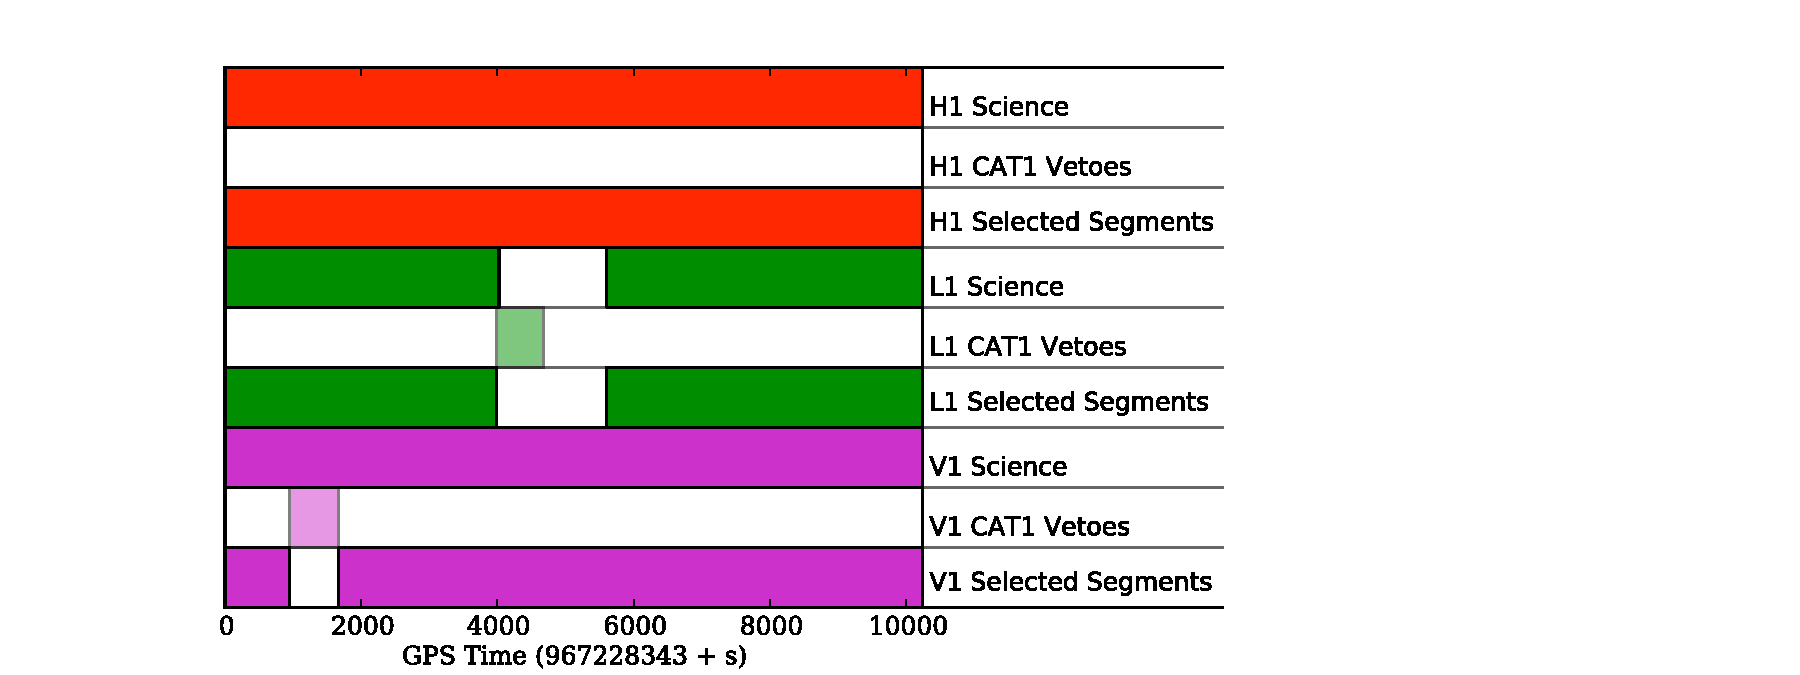
\includegraphics[width=6in]{figures/segment_plot_science-selected.pdf}
\end{center}
\caption{
The Science, category 1 vetoes, and selected segments of H1, L1, and V1 between GPS times 967228343 and 967238583.}
\end{figure}

\begin{figure}[p]
\label{fig:segment_plot_full}
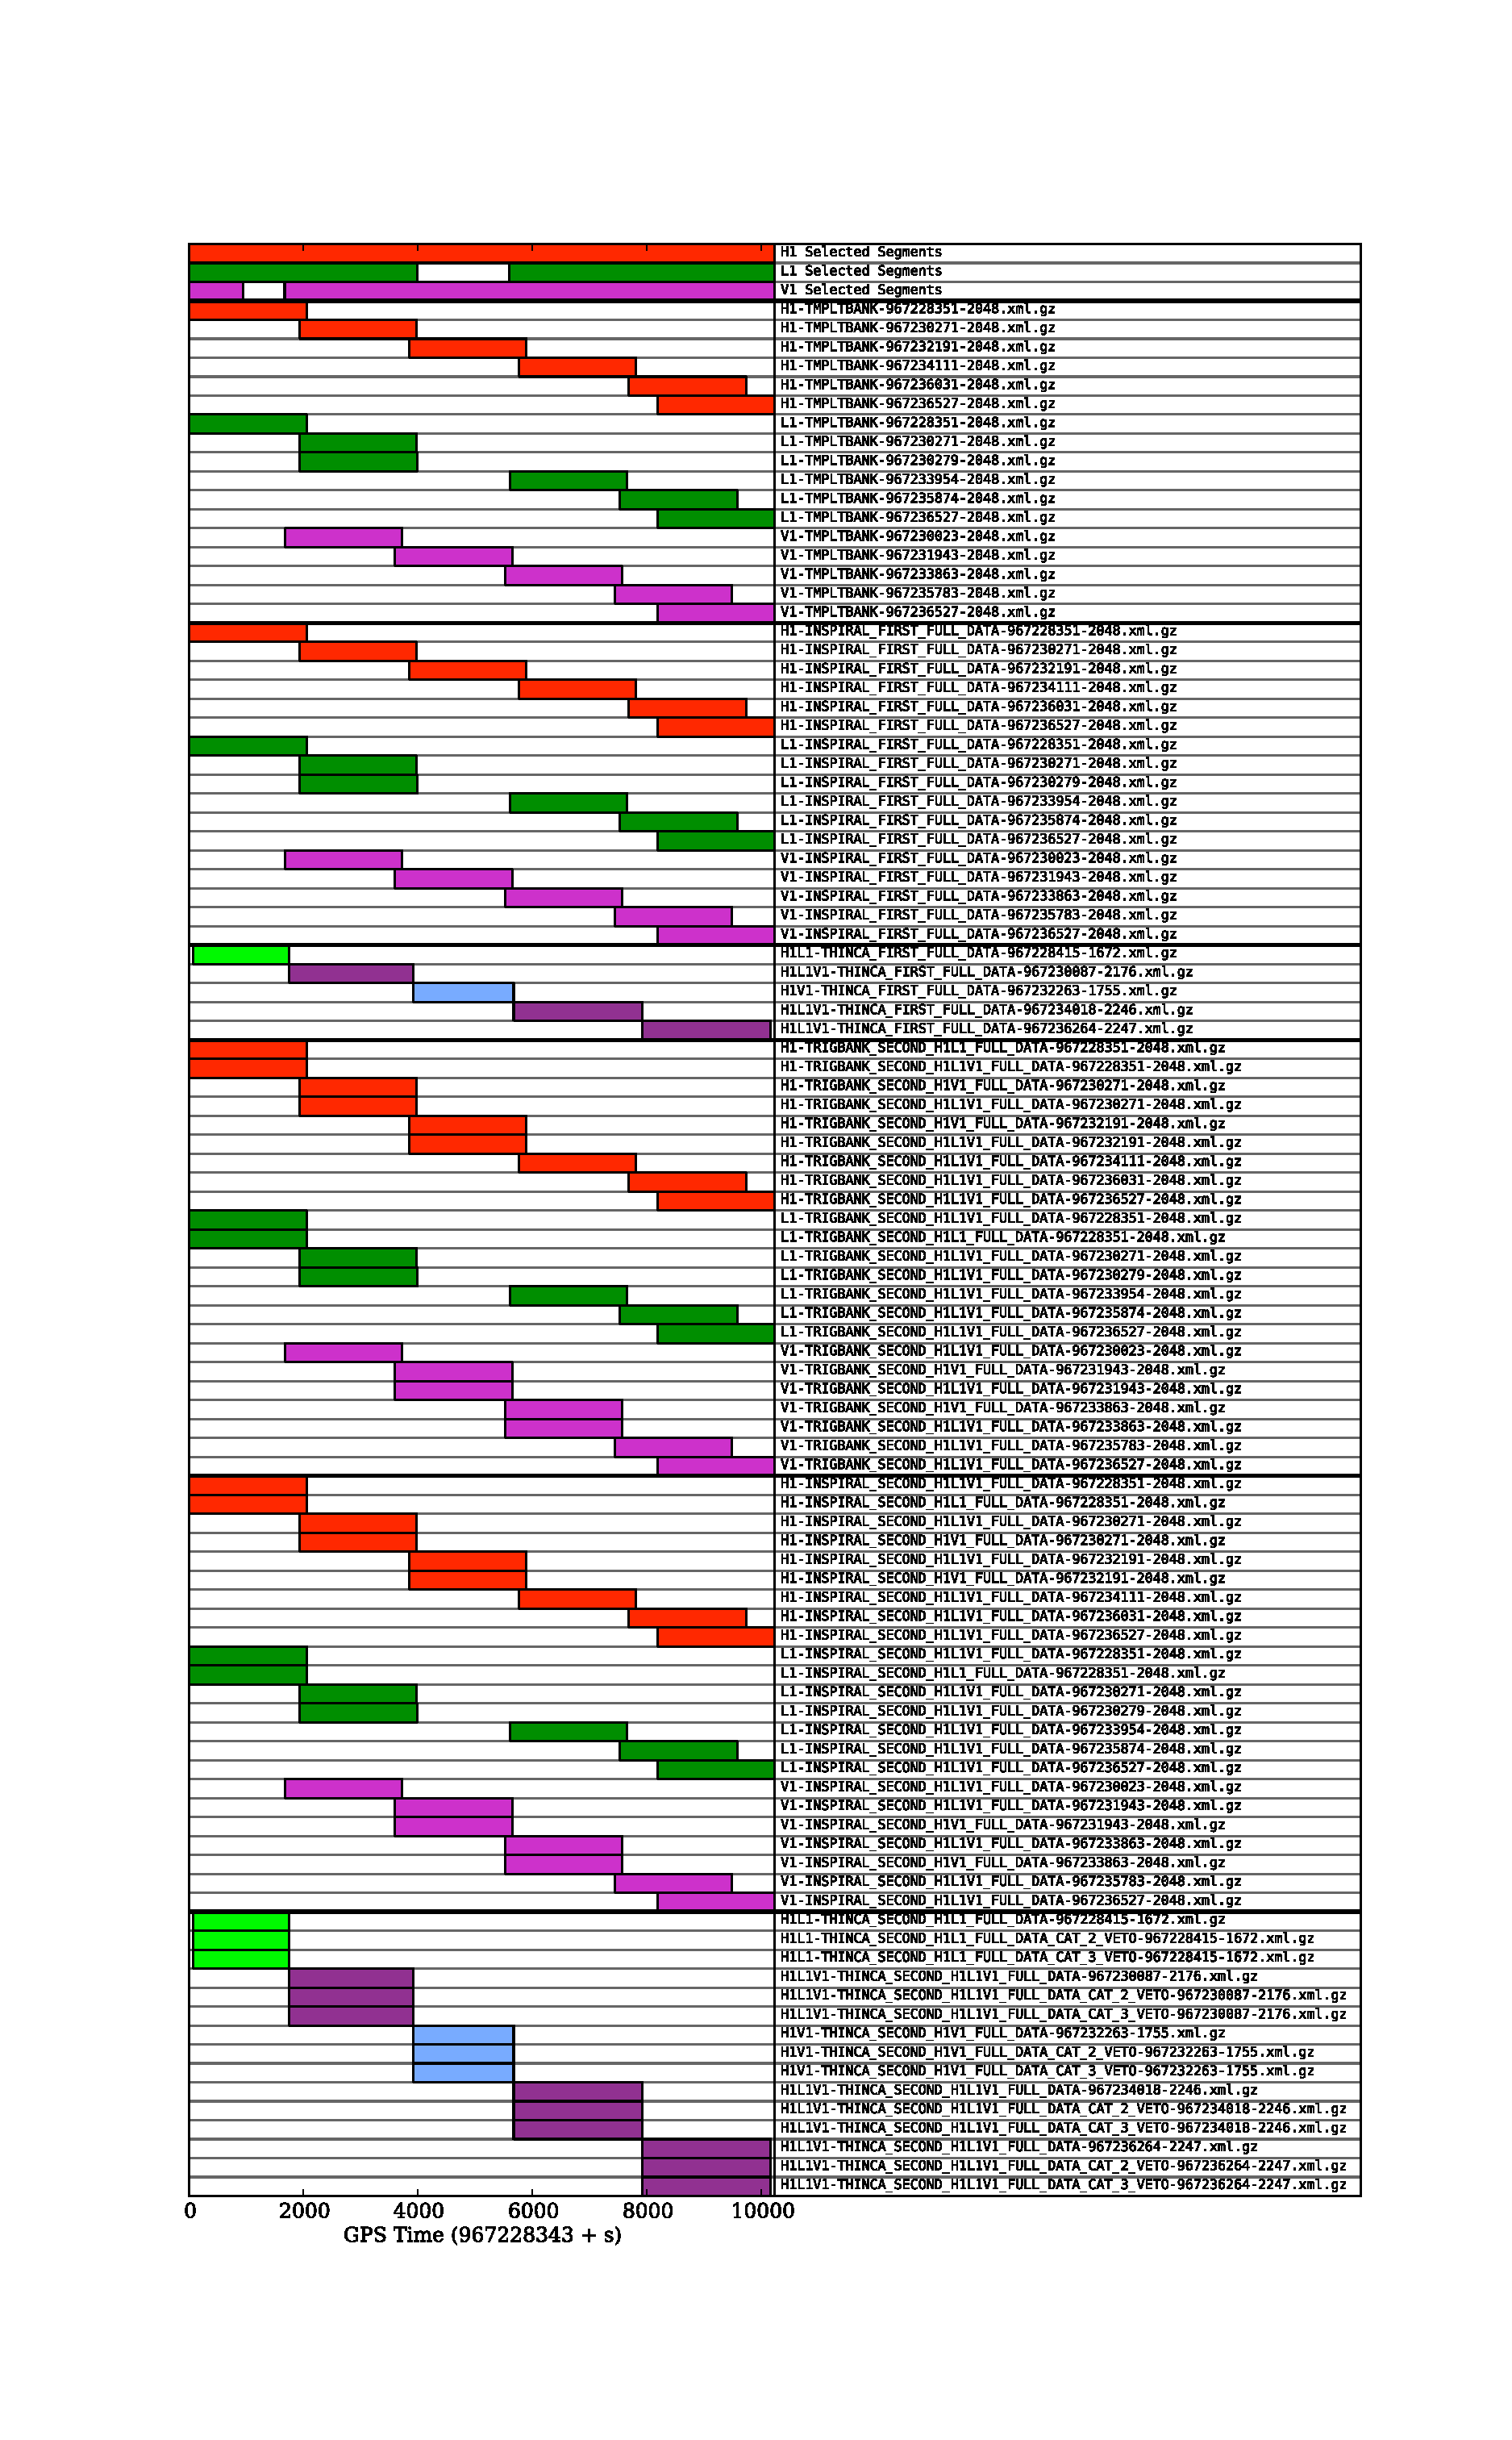
\includegraphics[width=6.5in]{figures/segment_plot_selected_segs-thinca_second.pdf}
\caption{
The selected segments and all zero-lag \texttt{FULL\_DATA} files created by \ac{HIPE} for the segments shown in Figure \ref{fig:science-selected_segs}.}
\end{figure}

\section{Data Storage}
\label{sec:data_storage}

Before stepping through Pipedown, we pause to detail the table structure used to store triggers in files. Table structure is central to Pipedown: part of its purpose is to convert from older table structures to newer, more convenient ones, and all the programs Pipedown runs take advantage of these newer tables. We begin by reviewing the \texttt{sngl\_inspiral} table, and how this was used to store data up to this point.

\subsection{The \texttt{sngl\_inspiral} Table}

As discussed above, the \texttt{sngl\_inspiral} table is the table used to store data by nearly every \ac{HIPE} program: \texttt{lalapps\_tmpltbank}, \texttt{lalapps\_inspiral}, and \texttt{lalapps\_thinca} all use it to store template and trigger information. Consequently, the \texttt{sngl\_inspiral} table has a large number of columns to store all needed data. Table \ref{tab:sngl_inspiral} shows some of the relevant columns used for the \ac{CBC} analysis and their purpose. There are several extra columns not discussed here.

Each row in the \texttt{sngl\_inspiral} table represents a single trigger or template in a single \ac{IFO}. Associated with each row is an \texttt{event\_id} to uniquely identify each event. This provides a convenient way to retrieve information about a template or single-\ac{IFO} trigger. Coincident information is more difficult to store, however, since coincidence requires grouping rows together. Since the \texttt{sngl\_inspiral} table was the only available way to store trigger data in a file when \texttt{lalapps\_thinca} was written, a method was devised to encode coincidence in the \texttt{event\_id}. The id was set to be 18 digits long. The first (starting from the left) 9 digits were the GPS time of the trigger. The next 4 digits gave the slide that the coincidence was from, where $0000$ was zero-lag. The last 5 digits formed a counter that assigned a unique number to each coincidence. For example, the first coincident trigger in H1L1 time in the first slide of our toy-analysis has \texttt{event\_id}:
\begin{equation*}
\underbrace{956735064}_{\text{GPS time}}\underbrace{0001}_{\text{slide number~}}\underbrace{00001}_{\text{~event counter}}
\end{equation*}
Any rows that had \texttt{event\_id}s with the same last 9 digits --- i.e., if the slide number and event counter matched --- were coincidences.

\subsection{The \texttt{sim\_inspiral} and \texttt{process} Tables}

Two other tables used by \ac{HIPE}, as well as Pipedown, are worth mentioning: the \texttt{sim\_inspiral} and \texttt{process} tables. The \texttt{sim\_inspiral} is similar to the \texttt{sngl\_inspiral} table. Instead of storing triggers, it stores lists of injections. Some of the columns of the table are shown in Table \ref{tab:sim_inspiral}. The table is indexed by the \texttt{simulation\_id}. This id is simply a number: no information is stored in it, as it is with the \texttt{event\_id}.

Note that both the \texttt{sim\_inspiral} and \texttt{sngl\_inspiral} table (as well as many other tables) have \texttt{process\_id} columns. These are used to map their entries to the \texttt{process} table. This table --- the columns of which are shown in table \ref{tab:process} --- is used to store relevant information about the program that created the entry. Associated with the \texttt{process} table is the \texttt{process\_params} table, which stores the arguments and values given to the program at run-time. For example, all the injections created by a single instance of \texttt{lalapps\_inspinj} will have the same \texttt{process\_id} in the \texttt{sim\_inspiral} table. These will all point to a single entry in the \texttt{process} table and multiple entries (one for each argument given to \texttt{lalapps\_inspinj}) in the \texttt{process\_params} table. These tables are useful for troubleshooting problems and verifying the correct program versions were used when an analysis was run. They are also used to associate a set of injections with a given injection \texttt{USER-TAG}; see section \ref{sec:dbaddinj} for details.

\subsection{Coinc Tables}

There were a few problems with using the \texttt{sngl\_inspiral} table to store coincident information. First, the number of coincident events in a single file could not exceed $99,999$, else the event counter would spill over into the slide number. Likewise, no more than $9999$ slides could be stored in a single file. Third, it consumed more memory than necessary. If a single-\ac{IFO} trigger formed coincidences in multiple slides (as is often the case), multiple entries would have to be created in the \texttt{sngl\_inspiral} table for it. The values in all columns (of which there are many) for these entries would be exactly the same, except for the last 9 digits of the \texttt{event\_id}. Finally, any coincident parameters, such as combined new \ac{SNR}, would have to be computed on the fly. For coincident statistics that could not easily be computed on the fly, such as \acp{FAR}, a \texttt{sngl\_inspiral} column (meant to store single information) had to be comandeered, and the same value would be stored repeatedly for each \ac{IFO} in the coincidence.

To remedy the situation, \emph{coinc tables} were developed. The coinc tables consist of the \texttt{coinc\_inspiral}, \texttt{coinc\_event}, \texttt{coinc\_event\_map}, and the \texttt{coinc\_definer} table. Additionally, there is the \texttt{time\_slide} table, although this is considered to be apart of the \emph{experiment} tables (see the next section). The columns in each of these tables and their purpose is shown in tables \ref{tab:coinc_inspiral} -- \ref{tab:time_slide}.

The \texttt{coinc\_inspiral} table is the coincident analog to the \texttt{sngl\_inspiral} table. Instead of storing single-\ac{IFO} information, the \texttt{coinc\_inspiral} table stores combined statistics and parameters. How information is combined depends on the parameter or statistic. Combined new \ac{SNR} is calculated by taking the quadruture sum of the constituent \ac{IFO}'s new \acp{SNR}, and is stored in the \texttt{snr} column.\footnote{Admittedly, storing combined new \ac{SNR}, not combined \ac{SNR}, in a column named \texttt{snr} is a little misleading. When the column names were defined, the \texttt{snr} column was intended to be a catch-all for whatever statistic was used to rank triggers. This way, multiple searches that may not use the same ranking statistic could use the same column. In retrospect, however, doing it in this manner was probably not needed, since SQLite allows columns to be added at will (see section \ref{sec:file_formats}). At the very least, the column probably should have been called something along the lines of \texttt{ranking\_stat}. Alas, hindsight is always 20/20.} Intrinsic parameters of the templates, such as chirp mass (stored in the \texttt{mchirp} column) and total mass (stored in the \texttt{mass} column), are combined by taking the mean of the of single-\ac{IFO} parameters. Coincident end times are computed by taking the end time from the first \ac{IFO} when sorted alphabetically. For example, in an H1L1 coincidence, the coincident end time will be whatever the H1 end time is. In an L1V1 coincidence, the L1 end time will be used. Similar to the original intent of the \texttt{event\_id}, a unique \texttt{coinc\_event\_id} is assigned to each coincidence in a file to provide a quick way to identify them. Additionaly, the \texttt{coinc\_event\_id} is used to map entries in the \texttt{coinc\_inspiral} table to entries in other tables. For every entry in the \texttt{coinc\_inspiral} table there is one entry in the \texttt{coinc\_event} table, as well as multiple entries in the \texttt{coinc\_event\_map} table with the same \texttt{coinc\_event\_id}.

The \texttt{coinc\_event\_map} table is used to map the coincident events in the \texttt{coinc\_inspiral} table to their constituent events in the \texttt{sngl\_inspiral} table. As can seen in table \ref{tab:coinc_event_map}, the \texttt{coinc\_event\_map} table has three columns: a \texttt{coinc\_event\_id}, an \texttt{event\_id}, and a \texttt{table\_name}. To map a single-\ac{IFO} trigger in teh \texttt{sngl\_inspiral} table to a coincident event, the single event's \texttt{event\_id} is entered in the \texttt{coinc\_event\_map} table next to the \texttt{coinc\_event\_id} of the coincidence it is part of. Likewise, all other single-ac{IFO} events that are apart of the coincidence will have entries in the \texttt{coinc\_event\_map} table with the same \texttt{coinc\_event\_id}. In this way, one coincident event is mapped to multiple single events. Likewise, a single \texttt{event\_id} does not have to be associated with one \texttt{coinc\_event\_id}. If a single event takes part in multiple coincidences it can also be added to the \texttt{coinc\_event\_map} table, with each entry being associated with a different \texttt{coinc\_event\_id}. By using an intermediate table we have allowed for many-to-many mappings between coincidences and single events. As a result, multiple entries do not have to be added to the \texttt{sngl\_inspiral} table, and the \texttt{event\_id}s no longer need to encode coincident information. \texttt{Event\_ids} are therefore changed to simple counters used to index the \texttt{sngl\_inspiral} table, so that each row has a unique id. This fixes the problem of counter-overflow; the number of events that can be stored in a single file is now only limited by disk or memory space.

Note that the table name from which a single event came --- in this case, the \texttt{sngl\_inspiral} table --- is also stored in the \texttt{coinc\_event\_map} table. This is done so that the \texttt{coinc\_event\_map} table can be used to draw multiple types of maps, e.g., it is also used to draw mappings between coincident events and injections. The manner in which injection mappings are drawn is more complicated, however; see section \ref{sec:inspinjfind} for details.

By changing the \texttt{event\_id} to a simple counter, we have also freed it from storing time-slide information. What slide an event belongs to is instead stored in the \texttt{time\_slide} table. As listed in table \ref{tab:time_slide}, the \texttt{time\_slide} table has an \texttt{ifo}, an \texttt{offset}, and a \texttt{time\_slide\_id} column. Each slide is given a unique \texttt{time\_slide\_id}; each slide id is repeated in the \texttt{time\_slide} table for every \ac{IFO} that was analyzed, with each row giving the offset (in seconds) applied to that \ac{IFO} in that slide. For example, if H1, L1, and V1 are being analyzed, and one of the slides has the offset vector given in equation \ref{eqn:example_offset_vec}, then that slide will have three entries in the time slide table:
\begin{center}
\begin{tabular}{ c | c | c }
time\_slide\_id & ifo & offset \\
\hline\hline
\texttt{time\_slide:time\_slide\_id:37} &   \texttt{H1}    & \texttt{0} \\
\texttt{time\_slide:time\_slide\_id:37} &   \texttt{L1}    & \texttt{15} \\
\texttt{time\_slide:time\_slide\_id:37} &   \texttt{V1}    & \texttt{30} \\
\end{tabular}
\end{center}
where we have assigned the slide the arbitrary id \texttt{time\_slide:time\_slide\_id:37}.\footnote{All ids have the basic format \texttt{[originating\_table]:[id\_name]:[index\_number]}. The index number is what makes each id unique within a given class.} Storing time-slides in this manner makes it easier to find what offset was applied to each \ac{IFO}, and it allows for non-multiple slide vectors should a new version of \texttt{thinca} be written. Coincident events (and, via the \texttt{coinc\_event\_map} table, single events) are mapped to time slides through two parallel tracts. One path is through the \texttt{coinc\_event} table; the other is by way the \texttt{experiment\_map} and \texttt{experiment\_summary} tables, which are discussed in the next section.

The \texttt{coinc\_event} table serves to store additional information about coincident events, as well as map events to other tables. Table \ref{tab:coinc_event} shows the \texttt{coinc\_event}'s columns. Every coincident event will have one entry in the \texttt{coinc\_event} table via their \texttt{coinc\_event\_id}. Since the table also has a \texttt{time\_slide\_id} column, it maps the events to their respective time-slides (a many-to-one mapping). The table additionally has an \texttt{instruments} column which gives the instrument time that the coincident event occurred in, which is important for computing \acp{FAR}. Instrument times are also stored in the \texttt{experiment} table, which is discussed in the next section. The \texttt{likelihood} column is used if a likelihood statistic is computed in a search. We do not do this in the low-mass \ac{CBC} search, however, and so it is unused. That it exists in the table is due to the fact that the \texttt{coinc\_event} table, along with the \texttt{coinc\_event\_map}, are search-independent tables. That is, they can be (and are) used by multiple search pipelines both within the \ac{CBC} group (such as the ringdown search) and outside of it; e.g., some burst searches use it. Contrast this with the \texttt{coinc\_inspiral} and \texttt{sngl\_inspiral} tables, which are specific to \ac{CBC} searches. An advantage of having search independent tables is that provides an easy way to store data if search is carried out that draws from multiple pipelines. Indeed, being able to combine results from multiple pipelines is an active field of research.

The \texttt{coinc\_event} table also maps coincident events to the \texttt{coinc\_definer} table via the \texttt{coinc\_def\_id} column. The \texttt{coinc\_definer} table is used to group together various types of mappings; its columns are shown in table \ref{tab:coinc_definer}. A human-redable description of the type of mappings is given in the \texttt{description} column. For example, all coincident events that are mapped to single-inspiral triggers will be associated with a single \texttt{coinc\_def\_id}. The entry in the \texttt{description} column for this id will be \texttt{sngl\_inspiral<-->sngl\_inspiral coincidences}. Mappings between injections (which are stored in the \texttt{sim\_inspiral} table) and coincident events will have a different \texttt{coinc\_def\_id}, and the \texttt{description} column will be \texttt{sim\_inspiral<-->coinc\_event coincidences}. The \texttt{coinc\_definer} table is therefore useful to grab coincidences formed by a specific method. For example, if two types of injection finding were being experimented with (say, a time-based method and an ethinca-ellipsoid based method), the \texttt{coinc\_definer} table would be needed to pick out which mappings occurred from which method. However, since the current low-mass \ac{CBC} search only performs one type of coincidence test and one type of injection finding (see section \ref{sec:inspinjfind} for details), the \texttt{coinc\_definer} table is largely unused by Pipedown programs.

\subsection{Experiment Tables}
\label{sec:experiment_tables}

The coinc tables solved many of the problems and difficulties of saving coincident information to a file. However, neither the older table structure nor the coinc tables provided a way to store information about the experiments performed. In particular, there was no way to store the live-time of a slide, nor the \emph{data type} of a trigger, i.e., whether the trigger came from playground data, data with playground excluded, time-slides, or an injection run. Initially, there was also no way to store what instrument time a trigger was in. This was amended by adding the \texttt{instruments} column to the \texttt{coinc\_event} table. However, this meant that information about an instrument time would only be stored in the file if an event occurred during it. If we perform an experiment and nothing happens during it, that is still information we want to keep. This is particularily true for computing false alarm rates: we need to know all the time that was observed in every slide, regardless of whether or not a slide produced an event. The only way to keep track of triggers' data types was to keep them in different files, and the only way to store livetimes was to store them in auxillary ASCII files. This could be confusing, and it forced meta-data to stored in file names.

For these reasons, the \emph{experiment} tables were developed. The experiment tables consist of the \texttt{experiment}, \texttt{experiment\_summary}, and \texttt{experiment\_map} tables. Their columns are listed in tables \ref{tab:experiment} -- \ref{tab:experiment_map}. The \texttt{experiment} table lists the experiments that were performed as well as information about each one. The \texttt{gps\_start\_time} and \texttt{gps\_end\_time} columns give the period across which the experiment was performed. In \ihope, these columns are set whatever the start and stop times were that were given to \ihope to analyze. The \texttt{search\_group} and \texttt{search} columns define what group performed the search (e.g., the \ac{CBC} group, or the Burst group) and what type of search was performed (e.g., \texttt{lowmass}). Since different instrument times are mutually exclusive, and since we do not calculate \acp{FAR} across them, every instrument time that was analyzed in the \texttt{search} by the \texttt{search\_group} between the GPS start and end times is listed as an independent experiment in the \texttt{experiment} table. Evidently, \texttt{experiment} not only lists the experiments performed, it \emph{defines} what an experiment is.

Within each experiment, we apply various vetoes, perform slides, and construct different data types (e.g., playground and injection runs). Each of these actions results in a different realization of an experiment. To define and list these realizations, we use the \texttt{experiment\_summary} table. Table \ref{tab:experiment_summary} shows the columns of the \texttt{experiment\_summary} table. Each row has its own \texttt{time\_slide\_id} and \texttt{experiment\_id} which maps it to the \texttt{experiment} and \texttt{time\_slide} table; thus, each row gives information about every slide that was performed in each instrument time. Additionally, there is a \texttt{datatype} column to enumerate each of the data types constructed in every experiment. This can have one of five entries: \texttt{all\_data}, \texttt{playground}, \texttt{exclude\_play}, \texttt{slide}, and \texttt{simulation}. The \texttt{all\_data}, \texttt{playground}, \texttt{exclude\_play}, and \texttt{simulation} are all zero-lag data types: \texttt{playground} is data consisting only of times occuring during playground seconds (defined above), \texttt{exclude\_play} is the converse, and \texttt{all\_data} consists of both. The \texttt{slide} data type is any non-zero lag data. We do not define a \texttt{slide} playground because playground slides are rarely used.\footnote{Looking at all-data slides is not considered opening the box.}

The \texttt{simulation} data type describes zero-lag data that has software injections in it. This allows us to easily separate injection runs from non-injection runs. In order to separate various injection runs we use the \texttt{sim\_proc\_id} column. The \texttt{process\_id} of the \texttt{lalapps\_inspinj} job that created a set of injections is stored in this column. All injections in a single injection run are created by a single \texttt{inspinj} job; thus all these injections will have the same \texttt{process\_id} in the \texttt{process\_id} column of the \texttt{sim\_inspiral} table. By storing the same value in the \texttt{sim\_proc\_id} column of the \texttt{experiment\_summary} table, we map the two tables together. Note that this mapping simply means that a given set of injections were performed during a realization of an experiment. It does not mean that all events that occured during that realization were from injections. To pick out what events were due to injections and which are due to noise, we rely on mappings in the \texttt{coinc\_event\_map} table.

The final mapping in the \texttt{experiment\_summary} table is the \texttt{veto\_def\_name} column. This column stores the name of a set of vetoes applied in the given realization of an experiment, e.g., \texttt{VETO\_CAT3\_CUMULATIVE} (the veto names are determined by \texttt{ligolw\_segments\_from\_cats}). This column maps the row to the \texttt{segment\_definer} table, which in turn maps to the veto segments, stored in the \texttt{segment} table. (See section \ref{sec:segment_tables} for more information on segment tables.) In this manner, the type of vetoes, and their segments, that were applied during an experiment can be retrieved without needing external files.

All of the \texttt{experiment\_summary} columns we have reviewed so far serve to categorize realizations of experiments. The \texttt{duration} and \texttt{nevents} columns, on the other hand, store data about a realization. Perhaps the most important column is the \texttt{duration} column. This column stores the amount of \emph{live time} that exists in an instrument time during the experiment period (again, stored in the \texttt{experiment} table and mapped to via the \texttt{experiment\_id}) for a given veto category in a given slide for a given data type. While the live time can be computed on the fly using information from the segment tables, it is not a trivial operation. It is therefore left to a single program to do (\texttt{ligolw\_cbc\_compute\_durations} --- see section \ref{sec:compute_durations} below) for all realizations, which stores the results in the \texttt{duration} column. This makes live time retrieval quicker and easier for other programs. The \texttt{nevents} column stores the number of coincident events that occurs during an experiment realization.

The final experiment table is the \texttt{experiment\_map} table. This table maps coincident events to realizations of experiments defined in the \texttt{experiment\_summary} table. It has two columns: an \texttt{experiment\_summ\_id} and a \texttt{coinc\_event\_id}. Having a table devoted solely to mapping coincident events and experiments allows for many-to-many mappings. This is needed: an experiment will have many events in it, and a coincident event can occur in multiple experiment realizations. For example, all zero-lag events will belong to the \texttt{all\_data} data type as well as either \texttt{playground} or \texttt{exclude\_play}. The \texttt{experiment\_map} allows all of these events to be efficiently stored in the same file, without needing to rely on file names to separate them. The effect of vetoes and which events survive which category --- a question that comes up often --- can also be acertained by simply looking at what mapping exist between a coincident event and \texttt{experiment\_summ\_id}s of various veto categories.\footnote{Currently, Pipedown stores different veto categories in separate files, and so checking veto categories via experiment tables is not currently taken advantage of. Combining vetoes into a single file is planned for the future, however.}

\subsection{The Segment Tables}

As they have already been mentioned a several times, and are used by several codes, we describe here the segment tables. The segment tables consist of the \texttt{segment}, \texttt{segment\_definer}, and \texttt{segment\_summary} tables. The columns of the \texttt{segment} and \texttt{segment\_definer} tables are shown in tables \ref{tab:segment} and \ref{tab:segment_definer}, respectively. The \texttt{segment\_summary} table is not shown nor described here, as it is not used by Pipedown programs.

The \texttt{segment\_definer} table serves to identify a collection of segments by name. For example, all of the CAT123 veto segments for a given \ac{IFO} will be given a single \texttt{segment\_def\_id} and have the name \texttt{VETO\_CAT3\_CUMULATIVE}. The start and end times of each segment in the collection are listed in the \texttt{segment} table; the mapping between segments and their grouping in the \texttt{segment\_definer} table occurs via the \texttt{segment\_def\_id}. As mentioned above, entries in the \texttt{experiment\_summary} table map to the veto segments applied via the name in the \texttt{segment\_definer} table. The mapping is not done using the \texttt{segment\_def\_id} because each \ac{IFO} will have its own entry, and therefore its own \texttt{segment\_def\_id}, in the \texttt{segment\_definer} table. Using these mappings, we can re-construct the periods of time vetoed in any realization or slide in an experiment.

\subsection{Other Tables}

There are many other tables in use by searches in the \ac{CBC} group as well as the rest of the \ac{LSC} in addition to the ones presented here. These include meta-data tables such as the \texttt{search\_summary} tables, as well as a large number of tables used by other searches and search groups. Since these tables have little, if any, impact on the low-mass \ac{CBC} search, we do not describe them here. For a complete list of all the tables, and their columns, see the \texttt{lsctables.py} code in the LALSuite repository. This can be accessed online at: \verb|{http://www.lsc-group.phys.uwm.edu/cgit/lalsuite/tree/glue/glue/ligolw/lsctables.py}|

\subsection{File Formats}

It will be useful to also make a note of the file formats used to store data. As mentioned in section \ref{sec:HIPEDetail} all \ac{HIPE} programs store data in xml files. This is convenient because xml files can opened, looked at, and edited using any text editor; at the same time, they provide a standard format that can be interpetted by code.

The downside to xml files is that the entire file must be loaded by a program in order to parse its data. This puts a limit to how much data can be stored in a file, and has proven to be troublesome when computing statistics, such as \acp{FAR} that require a large swath of data. It also means that many files can only be handled by computers with large amounts of memory, which limits the number of nodes in a cluster a that a program can be executed on. Even then, periods of high glitch rate occasionally max out memory, thus requiring more aggressive clustering. Finally, it can be difficult to quickly sort through large amounts of data to find a few triggers of interest, such as the ones with the smallest \ac{FAR}. Doing so requires writing code that can filter through large numbers of files as well as access to library packages that know how to interpet \ac{LIGO}-Virgo xml files.

For these reasons, Pipedown converts xml files to SQLite databases, which are used by a number of its programs. SQLite has a number of advantages. Database files remain on disk: when a program reads from a database, it does not need to load the database into memory. Instead, it queries only the information it needs to perform a specific task. Once an operation is completed on that data, the results can be dumped back to the database and cleared from memory. Thus, file size is limited only by disk space, of which there is far more --- and which is much cheaper --- than memory. SQLite is also fast: it automatically invokes a number of optimization schemes which allows it to quickly read and write data, without needing special commands. Thus, when coding, we can concentrate more on what to do with data rather than how to get it. SQLite is also flexible. With xml, what columns exist in a table must be defined in \verb|lsctables.py|. The only way extra columns can be added is to edit \verb|lsctables.py| to add the column, re-install it, then re-create the xml. This can be frustrating when doing investigations into new statistics. SQLite, on the other hand, does not use table definitions. It can create new columns on the fly and add them to any table in the database. This is taken advantage of by a number of Pipedown programs, such as \verb|ligolw_cbc_repop_coinc| and \verb|ligolw_cbc_cfar|; see their respective sections for details. Finally, SQLite is well supported: it is developed and maintained by dedicated professional programmers, while also being open-source \cite{ref:SQLiteSite}. There exists a Python package for it so that it can be used from within Python code, even though SQLite itself is written in C. Additionally, there exists a free SQLite command-line tool (installed on all the \ac{LIGO} clusters) which can parse a database without needing support code to read data tables, as is the case with xml. One can therefore quickly search data from the command line without needing to hand-write tools.

The downside to SQLite is database files are not human-readable. Either the command-line tool must be used to see data, or code must be written to print data out. Additionally, while the flexibility to create arbitrary columns on the fly is useful for investigations, once a statistic has been settled on, we wish to standardize the column. Otherwise it could be difficult to know what is stored where when going back over results created by different people at different times. For these reasons, xml files are considered to be the ``final" data products produced by the \ac{CBC} pipeline. One of Pipedown's goals is to take all the data analyzed by \ihope and disseminate it down to a few xml files containing a handful of ``loudest" triggers that are of interest.

\section{Pipedown in Detail}

We now step through Pipedown in detail, using Figure \ref{fig:PipedownDetail} and our toy analysis as a guide. Pipedown is run after all \ac{HIPE} runs have completed. It combines data from all these runs --- including zero-lag, time-slides, and all injection runs --- into a single database. \acp{FAR} are calculated using this database, and a number of plots are generated using it. Although the experiment table structure allows multiple veto categories to be stored in a single database, Pipedown currently keeps each veto category in a separate database. Thus, the pipeline shown in Firgure \ref{fig:PipedownDetail} is repeated for each veto category.

\subsection{\texttt{ligolw\_thinca\_to\_coinc}}

The first program run in Pipedown is \texttt{ligolw\_thinca\_to\_coinc}. It reads second \texttt{THINCA} files, and uses \texttt{sngl\_inspiral} \texttt{event\_id} to construct coinc and experiment tables, as well as convert the \texttt{event\_id} to a counter. It also loads the veto segments file corresponding to the given category that was produced by \ihope at run time. The veto segments are used to figure out what instrument times triggers belong to. (As discussed in the Second Thinca section, when higher category vetoes are applied, some coincidences will be moved to a different instrument time than what is indicated in the file name. \texttt{Thinca} does not store this information, so it must be reconstructed.) Although the veto segments (which are stored in segment tables), the veto segments are not added to the output xml file. Doing so at this point would cause repition across the files that would have to be remedied when the files are combined into a database. For simplicity, the veto file is added to the database at a later point.

When applying vetoes to check instrument times, there are occasional edge cases in which more \acp{IFO} can be coincident than there are instruments on. For example, a H1L1V1 trigger can appear to occur duing H1V1 time. This is due to the way end times are recorded: as described above, the coincident end time is chosen to be the end time of the first \ac{IFO} when sorted alphabetically by name. So, in our example, the coincident end time is whatever the H1 trigger's end time is. Coincident windows have some spread in time, however, so this end time only represents a (somewhat arbitrary) point during that window. If a veto turns on during the window, the trigger on which the end time is based can be coincident with a trigger in the \ac{IFO} that is vetoed, if the trigger happened just before the veto. So, in our example, a L1 trigger must have occurred just before a L1 veto. The H1 trigger occurred just after the L1 veto, and so the end time of the H1L1V1 trigger appears to occur during H1V1 time. In this case, \texttt{ligolw\_thinca\_to\_coinc} assigns the trigger to H1L1V1 time.

For non-injection runs, \texttt{thinca\_to\_coinc} combines the zero-lag and slide second \texttt{THINCA} files into a single xml file. Thus, for every two \texttt{FULL\_DATA} second \texttt{THINCA} files, there is one \texttt{THINCA\_TO\_COINC} file. The output file has the same naming convention as the second \texttt{THINCA} files, except \texttt{THINCA\_(SLIDE\_)SECOND} is replaced with \texttt{THINCA\_TO\_COINC}.

In addition to constructing coinc and experiment tables, \texttt{ligolw\_thinca\_to\_coinc} also computes some coincident parameters, storing them in the \texttt{coinc\_inspiral} table. The includes the end time, combined chirp mass, combined total mass, and combined new \ac{SNR}.

\subsection{\texttt{ligolw\_sqlite}}

The next step in the Pipedown pipeline is to convert xml files to SQLite databases. This is done by \texttt{ligolw\_sqlite}. As can be seen in Figure \ref{fig:PipedownDetail}, \texttt{ligolw\_sqlite} turns all of the \texttt{thinca\_to\_coinc} xml files sharing a common \texttt{USER-TAG} into one database. (Blue arrows on the diagram indicate SQLite databases; black arrows indicate xml files.) The naming convention for the output database is:
\begin{center}
\begin{footnotesize}
\begin{verbatim}
{ANALYZED-IFOS}-{USER-TAG}_CAT_{N}_VETO_RAW_CBC_RESULTS-{GPS-START}-{DURATION}.sqlite
\end{verbatim}
\end{footnotesize}
\end{center}
where \texttt{ANALYZED-IFOS} are all the \acp{IFO} that are in the database, \texttt{N} is veto category\footnote{Note: in keeping with the \ac{HIPE} naming conventions, for CAT1 databases, the \texttt{CAT\_N\_VETO\_} part of the file name is excluded.}, \texttt{GPS-START} is the \ihope start time, and \texttt{DURATION} is the \ihope duration. For example, in our toy analysis, we would have two CAT3 databases:
\begin{center}
\verb|H1L1V1-FULL_DATA_CAT_3_VETO_RAW_CBC_RESULTS-967228343-10240.sqlite|
\end{center}
and
\begin{center}
\verb|H1L1V1-BNSINJ_CAT_3_VETO_RAW_CBC_RESULTS-967228343-10240.sqlite|
\end{center}
At this point the \texttt{FULL\_DATA} database contains both zero-lag and slide data.

In addition to being able to add xml files to a database, \texttt{ligolw\_sqlite} can also extract xml files from databases. As a result, it is used many times in Pipedown to go between SQLite databases and xml files, as can be seen in Figure \ref{fig:PipedownDetail}.

\subsection{\texttt{ligolw\_cbc\_dbsimplify}}

Id columns must be unique in a single file. For example, there can only be one coincident event in the \verb|coinc_inspiral| table with \verb|coinc_event_id coinc_event:coinc_event_id:0| in a given file. Since the ids are simply counters, however, there is no way to ensure that they are unique across files. Thus, when \verb|ligolw_sqlite| combines xml files into a single database, it has to increment all the table ids to prevent ``collisions." For example, if a coincident event in the database already has \verb|coinc_event_id coinc_event:coinc_event_id:0|, and we wish to add another \verb|THINCA_TO_COINC| file that also has a coincident event with \verb|coinc_event_id coinc_event:coinc_event_id:0|, this latter id will be incremented to one plus whatever the largest id is in the database. The same goes for all other ids. This ensures that independent entries across files remain independent when combined into a single database or file.

However, we may not wish to keep all entries independent when combining files. For example, all the \verb|THINCA_TO_COINC| files in a single \ihope run will have the same entries in the \verb|experiment| table. When \verb|ligolw_sqlite| adds all of these files into a single database, it will keep all of the entries independent by incrementing the \verb|experiment_id|s. In our toy analysis --- in which we have five \verb|FULL_DATA THINCA_TO_COINC|, with each one containing four \verb|experiment| entries (one for each possible instrument time) --- each \verb|experiment| entry will be repeated five times in the \verb|FULL_DATA THINCA_TO_COINC| database, leading to 20 total entries when we should only have 4. The same is true of any other table that stores information that spans multiple \verb|THINCA_TO_COINC| files, including the \verb|experiment_summary|, \verb|time_slide|, and \verb|coinc_definer| tables. The same is also true of the \verb|veto_definer|, \verb|sim_inspiral|, and segment tables. However, as these tables only exist in the veto file and the \verb|INJECTIONS| file, we avoid having to deal with them by adding them to the database after all the \verb|THINCA_TO_COINC| files have been added.

To remove these redundancies, \verb|ligolw_cbc_dbsimplify| is run. This program loads a database created by \verb|ligolw_sqlite| and removes any redundant entry from the \verb|experiment|, \verb|experiment_summary|, \verb|time_slide|, and \verb|coinc_definer| tables. It then updates the corresponding ids in all other tables to point to the correct entry. This is done in-place, i.e., the output database has the same name as the input database. Due to the redundancy problem, \verb|ligolw_cbc_dbsimplify| should always be run after \verb|ligolw_sqlite| is used to add files to a database.

\subsection{ \texttt{ligolw\_cbc\_repop\_coinc} }

After all the \verb|RAW| databases have been created and simplified, Pipedown runs \verb|ligolw_cbc_repop_coinc|. This program reads single-\ac{IFO} information from the \verb|single_inspiral| table, compute a specified combined statistic, and saves it in the \verb|coinc_inspiral| table. For example, if told to compute combined \ac{SNR}, it will calculate the quadruture sum of the single-\acp{IFO}' \acp{SNR} and save it to the \verb|coinc_inspiral| table. If told to compute combined chirp mass, it will calculate the mean single-\ac{IFO} chirp mass and save it.

What column \verb|repop_coinc| saves the combined parameter to is specified using the \verb|output-column|. \verb|Repop_coinc| takes advantage of SQLite's ability to create new columns in a table. The column does not need to already exist in the \verb|coinc_inspiral| table, nor does it need to be apart of the ``blessed" columns specified in the table definitions in \verb|lsctables.py|. If the column does not exist, \verb|repop_coinc| will simply create it, then store the data. If the column does exist, the data in it will be overwritten. This makes \verb|repop_coinc| extremely useful for experimenting with new statistics: one can take a database created by Pipedown, and add to it any statistic they wish without needing to update and re-install the LALSuite code base. Since the experimental statistic can be added to the \verb|coinc_inspiral| table, it can sit alongside currently used statistics (i.e., older data need not be overwritten), which makes it easy to compare the new statistic to older ones. However, columns that are not in the table definitions in \verb|lsctables.py| will not be in xml files that are extracted from a database. Therefore, if column is going to be used long-term, it should be added to list of ``blessed" columns.

As \verb|thinca_to_coinc| already populates most of the \verb|coinc_inspiral| columns needed by the low-mass \ac{CBC} search, \verb|repop_coinc| is currently bypassed in the low-mass pipeline. However, as new statistics are invented or desired parameters are added, they will be computed by \verb|repop_coinc| rather than \verb|thinca_to_coinc|. This is partly because \verb|thinca| and \verb|thinca_to_coinc| are planned to be phased out in favor of a single coincidence program that uses the coinc and experiment table structure natively. The primary purpose of such a program is simply to find coincidences; once coincidences have been drawn, it will be left to \verb|repop_coinc| to compute and store all combined statistics.

\section{\texttt{ligolw\_cbc\_cluster\_coincs}}

Although we apply some bank-wide clustering in \verb|lalapps_inspiral|, experience has taught us that a single event can still cause many triggers after \verb|inspiral|'s clustering. Further, because it does not compute new \ac{SNR}, bank clustering in \verb|lalapps_inspiral| is based on \ac{SNR}. We therefore try not to be too agressive with clustering in \verb|inspiral|, as it may not necessarily pick the best candidate. Instead, we do a final round of bank-wide clustering in Pipedown using \verb|ligolw_cbc_cluster_coincs|.

\verb|Cluster_coincs| clusters triggers based on combined statistics in the \verb|coinc_inspiral| table. What statistic it uses is determined by the \verb|ranking-stat| argument, set in the configuration file. In the low-mass \ac{CBC} search we use combined new \ac{SNR}.\footnote{In addition to \texttt{ranking-stat}, there is another argument, \texttt{rank-by}, which tells \texttt{cluster\_coincs} whether to cluster on large values of the ranking-stat, or small values. Thus, the program can cluster using statistics in which larger is better, such as new \ac{SNR}, or ones in which smaller is better, such as \ac{FAR}.} The clustering is done using a sliding time window in a similar manner as max-over chrip length: if there is another trigger within $\pm t_{\mathrm{win}}$ of a given trigger's end time with a ranking-stat value greater-than it (or less-than it --- see footnote), the trigger is deleted. The difference from max-over chirp-length is that the time window, $t_{\mathrm{win}}$, used by \verb|cluster_coincs| is a fixed value set in the configuration file. In the low-mass \ac{CBC} search we set the window to $10\,$s for both \ac{S5} and \ac{S6}.

Since all slides and zero-lag, as well as playground, all-data, and exclude-play, triggers exist in the same database, the \verb|experiment_map| table is used to ensure the triggers are only clustered within their slides and datatype. We do not wish to cluster triggers across datatypes: it is possible for a trigger to survive clustering in playground, but be clustered away in all-data. Thus, clustering is carried out by first deleting mappings between coincident events and \verb|experiment_summ_id|s in the \verb|experiment_map| table; only events with the same \verb|experiment_summ_id| are compared to each other.\footnote{As a result, events must also be in the same instrument time for them to be clustered together.} Events that have no mappings left to any \verb|experiment_summ_id| are deleted entirely from the database.

In addition to binning events by datatype, slide, and instrument type, \verb|cluster_coincs| can optionally bin by a coincident parameter and coincidence type. Two arguments can govern binning by a parameter range: \verb|param-name|, which sets what column in the \verb|coinc_inspiral| table to use, and \verb|param-ranges|, which set the values to bin by. For coincidence type, \verb|cluster_coincs| can be told to bin by the \acp{IFO} that took part in the coincidence (using \verb|group-by-ifos|), or the \emph{number} of coincident \acp{IFO} (using \verb|group-by-multiplicity|). For example, if \verb|group-by-ifos| is set, H1L1 and L1V1 triggers would not be clustered together. If \verb|group-by-multiplicity| is set, H1L1 and L1V1 triggers would be clustered together, but H1L1V1 triggers would not. If neither is set, all types are clustered together. These same arguments are used by several other programs to bin triggers, including \verb|ligolw_cbc_cfar| and a number of the plotting programs.

In both \ac{S5} and \ac{S6} triggers were grouped by \acp{IFO} when being clustered. In \ac{S6} triggers were additionally grouped into the same chirp-mass bins that are used to compute uncombined \acp{FAR} (see section \ref{sec:cfar} for the bin boundaries). We chose to cluster in chirp-mass bins out of concern that higher trigger rates and larger new \acp{SNR} in one bin would cause triggers that would otherwise have lower uncombined \acp{FAR} to be lost in other bins. This would negate some of the benefits of binning triggers when computing \acp{FAR}. However, as a result of this choice, a loud event that rang off triggers in all bins would have three candidate triggers: one in each bin. In this case, we resolved to use the trigger that had the lowest uncombined \ac{FAR}. If a trigger was loud enough to have a \ac{FAR}$= 0$ in multiple bins, we would try to measure a \ac{FAR}, either by doing more slides or by folding in data from other runs. If a \ac{FAR} could still not be determined, we would use the one with the largest new \ac{SNR}. These considerations became important in the investigation of the blind injection made during \ac{S6}; see Chapter \ref{ch:s6_results} for details.

As seen in Figure \ref{fig:PipedownDetail}, \verb|cluster_coincs| runs separately on each \verb|RAW| database. It writes the results to a new database which has naming convention:
\begin{center}
\begin{footnotesize}
\begin{verbatim}
{ANALYZED-IFOS}-{USER-TAG}_CAT_{N}_VETO_CLUSTERED_CBC_RESULTS-{GPS-START}-{DURATION}.sqlite
\end{verbatim}
\end{footnotesize}
\end{center}
In our toy analysis we thus have two clustered databases at CAT3:
\begin{footnotesize}
\begin{center}
\verb|H1L1V1-FULL_DATA_CAT_3_VETO_CLUSTERED_CBC_RESULTS-967228343-10240.sqlite|
\end{center}
\end{footnotesize}
and
\begin{center}
\begin{footnotesize}
\verb|H1L1V1-BNSINJ_CAT_3_VETO_CLUSTERED_CBC_RESULTS-967228343-10240.sqlite|
\end{footnotesize}
\end{center}

\subsection{The Injection Branch}

At this point in Pipedown, additional steps are carried out on the \verb|CLUSTERED| injection databases that are not carried out on the \verb|FULL_DATA| database. First, \verb|ligolw_cbc_dbaddinj| is run on each injection database. This adds the \verb|INJECTIONS| file that was created by \verb|lalapps_inspinj| to the database with the corresponding \verb|USER-TAG|. Included in the \verb|INJECTIONS| file is the \verb|sim_inspiral| table. The same code that \verb|ligolw_sqlite| uses to add files to databases is used by \verb|dbaddinj|. We do not need to run \verb|dbsimplify| after it, however, because there are no tables in the \verb|INJECTIONS| file that will lead to redundancies when added to the database. We do not use \verb|ligolw_sqlite| to add the file because, in addition to adding the \verb|INJECTIONS| file, \verb|ligolw_cbc_dbaddinj| updates the \verb|sim_proc_id| column of the \verb|experiment_summary| table with the \verb|process_id| of the instance of \verb|insinj| that created the injections.

After \verb|dbaddinj| is run, \verb|ligolw_sqlite| is run to convert each injections database into a single xml file. The name of the xml files are the same as the \verb|CLUSTERED| database, except the \verb|.sqlite| file extension is replaced with \verb|.xml|. This conversion must be done because the next program, \verb|ligolw_inspinjfind|, can only read xml files.

\verb|Ligolw_inspinjfind| performs \emph{injection finding}: it maps injections that were perfomed to triggers that were caused by the injection. To decide whether or not a trigger was created by an injection \verb|inspinjfind| uses a $1\,$s time window; i.e., any coincident trigger that occurs within $\pm 1\,$s of an injection is considered to have been caused by that injection. Note that this means that multiple events can be mapped to a single injection. Simply using a time window does increase the chance for random noise events to get mapped to an injection. We use such a large window for purposes of calculating upper limits. When calculating upper limits we are only interested in injections that are louder than the loudest event. Since (in principle) the only difference between the \verb|FULL_DATA| results and the simulation runs are the injections, any event in the simulation runs that is louder than the loudest full-data event must be from an injection. Thus, we are safe simply using a time window for calculating upper limits. Admittedly, however, this method is not ideal when using injections to tune the pipeline. For that, an ethinca-ellipsoid based approach might be better. Investigations into implementing such a method are planned.

\verb|Inspinjfind| works on the xml file in place; i.e., the mappings are added directly to the file. The maps between the injections (stored in the \verb|sim_inspiral| table) and coincident event are stored in the \verb|coinc_event_map| table. How exactly the maps are done is more complicated than how single-\ac{IFO} events are mapped to their coincident counterparts; we do not discuss it here. For details, see the \verb|ligolw_inspinjfind| golassary entry on the web at \verb|{https://www.lsc-group.phys.uwm.edu/ligovirgo/cbcnote/ligolw_inspinjfind}| (authentication required).

\subsection{Preparing the Final Database}

After \verb|lalapps_inspinjfind| has run on each of the injection xml files, they are added to the \verb|FULL_DATA CLUSTERED| database. This is done by \verb|ligolw_sqlite| followed by \verb|ligolw_cbc_dbsimplify|. Next the veto xml file (the same one given to \verb|thinca_to_coinc|) is added to the database. Thus, the \verb|FULL_DATA CLUSTERED| database contains all triggers from the zero-lag, slide, and injection runs, as well as all injection made (both ``found" and ``missed") in all runs, and the veto segments applied to the run. The \verb|FULL_DATA CLUSTERED| database is therefore the final data product from the pipeline: it is from this that false alarm will be computed (and saved) and all plots will be generated. The other databases --- i.e., all of the \verb|RAW| and injection databases --- are only intermediate data products.

Now that the veto segments are in the database, \verb|ligolw_cbc_compute_durations| is run to compute the live time in each slide and zero-lag. To do the computation, \verb|compute_durations| must know what times were analyzed (pre-vetoes). It gets this from the \verb|thinca| start and stop times, which is stored in one of the meta-data tables (specifically, the \verb|search_summary| table, which is not described here). The \verb|thinca| start and stop times are needed because these define the ring boundaries within which triggers and vetoes were slid around. For each entry in the \verb|experiment_summary| table, the single-\ac{IFO} veto segments are retrieved (using the \verb|veto_def_name| column to get the appropriate segments from the \verb|segment| table) then slid around on the \verb|thinca| rings according to the offset vector associated with the entry (retrieved from the \verb|time_slide| using the \verb|time_slide_id| column). Subtracting the duration of the vetoes from the total analysis time gives the live time of the entry. For the \verb|playground| and \verb|exclude_play| datatypes, the playground segments (computed from the GPS times) are additionally intersected with the segments. The results are saved to the \verb|duration| column of the \verb|experiment_summary| table.

\subsection{Computing False Alarm Rates}

All of the pieces are now in place in the \verb|FULL_DATA CLUSTERED| database to compute the \acp{FAR} of the triggers. Both the uncombined and combined \acp{FAR} are calculated using \verb|ligolw_cbc_cfar|. cFar is run twice. On the first pass, the \verb|group-by-ifos|, \verb|param-name| and \verb|param-ranges| arguments are given to cFar, which causes it to compute the uncombined \acp{FAR}. As outlined in the algorithim at the end of Chapter \ref{ch:far}, the \ac{FAR} for each trigger is calculated by counting the number of background triggers in the same \ac{IFO} and chirp-mass bin that have a new \ac{SNR} greater-than-or-equal to it. Specifically, cFar uses the \verb|experiment| and \verb|experiment_summary| tables to grab all of the \verb|slide| triggers in each instrument-time, and it uses the \verb|ifos| and \verb|mchirp| columns in the \verb|coinc_inspiral| table to apply the bins. The background time is retrieved by summing the \verb|slide| \verb|exerpiment_summary| entries' live time. For \verb|slide| triggers, triggers nor live time within that slide are used to compute their \acp{FAR}. The uncombined \acp{FAR} are saved to the \verb|false_alarm_rate| column of the \verb|coinc_inspiral| table.

Combined \acp{FAR} are computed when \verb|ligolw_cbc_cfar| is run again. This time, triggers are not binned by chirp mass or coincident \acp{IFO}, and the uncombined \acp{FAR} computed on the first pass are used as the ranking statistic. This result is saved to the \verb|combined_far| column of the \verb|coinc_inspiral| table.

With the completion of the second cFar job, the \verb|FULL_DATA CLUSTERED| databases have obtained their final form. All other jobs launched by pipedown either create plots, summarize the most significant events in short lists, or run followups on loud triggers. The programs that carry these out are described in the next few sections.

\subsection{IFAR Plots}

Pipedown launches several plotting programs to summarize the results for analysts. Perhaps the most significant is \verb|ligolw_cbc_plotifar|. PlotIFAR creates cumulative histograms of the triggers as a function of the \emph{inverse} false alarm rate, or IFAR. Plots are created of both inverted uncombined \ac{FAR} and combined \ac{FAR}; figure \ref{fig:sample_plotifar} shows a sample of each. Both plots show the excpected background distribution, which is simply 1/IFAR, as a dashed black line. The yellow regions show the expected background $\pm \sqrt{N}$ and $\pm 2\sqrt{N}$ where $N$ is the number of counts. These regions are the expected variance of the background, which at high $N$ corresponds to the 1 and 2 $\sigma$ significance bands in a Gaussian distribution. The gray lines show the actual background distribution: each line represents a single slide.\footnote{Note that the actual background appears to disagree with the expected variance (yellow regions) at high IFAR. This is due to the difference between Gaussian and Poisson distributions. At low $N$ the Poisson distribution becomes asymmetric around the mean, so that the variance does not agree with the familar 1 and 2 $\sigma$ bands of a Gaussian. If the yellow regions mapped out $\sigma$ instead of variance (i.e., if they mapped out the regions we expect $\pm 34\%$ and $\pm 47.5\%$ of the triggers to fall) then they would appear to agree with the gray lines.} The zero-lag distribution is plotted by the colored symbols. In the uncombined plot, the symbols are determined by the chirp-mass bin they represent and the color is determined by the coincident \acp{IFO}. The dashed colored lines show where the background for a particular \ac{IFO} combination (represented by the lines' colors) and chirp-mass bin (represented by the dash pattern) ``runs out"; i.e., they are points of maximum (minimum) background \ac{FAR} (IFAR). The uncombined plots are useful for understanding characteristics of the data. For example, we do not see any high mass H1L1V1 triggers (purple squares) in the plot. This is expected, because we can see that the background for high mass H1L1V1 triggers (the purple dashed line furthest to the right) runs out at an IFAR greater than the expected background at a cumulative number equal to one. Thus the probability of getting a triple-coincident high mass trigger in a single experiment realization is less than one. In the combined plot, all zero-lag triggers are plotted as blue triangles.

If a trigger is louder than all the background it will have a \ac{FAR} equal to zero. As discussed in Chapter \ref{ch:far}, this means that we have placed an upper limit on the \ac{FAR} equal to $1/\mathrm{T_b}$ where $\mathrm{T_b}$ is the total background time. On IFAR plots, zero-\ac{FAR} triggers are therefore placed at the point corresponding to $x=\mathrm{T_b}$\footnote{Since the loudest background trigger will always have a zero-FAR, this point can be seen in the combined plot where the gray lines end; in the uncombined plot the point is marked by the solid black line.} and an arrow pointing to the right is added to the trigger to indicate that the true IFAR is somewhere in the region to the right. Such triggers are of utmost interest to us; the first thing we look for when looking at an IFAR plot is whether or not any trigger is louder than all the background.

Since the combined IFAR plot quickly conveys whether or not a trigger is louder than all the background --- i.e., whether or not there is a \ac{GW} candidate --- as well as how signficant triggers are and how well the zero-lag distribution is consistent with the background, it is our primary detection plot. When we open boxes it is the first thing we look at. For example, in the sample combined IFAR plot shown in Figure \ref{fig:sample_plotifar_combined}, we see that the loudest zero-lag event has a IFAR of $\sim0.02$, corresponding to a \ac{FAR} of $\sim50$ per year. There is therefore no \ac{GW} candidate in this data. Additionally, since the zero-lag is consistent with background across the entire region, we can be fairly confident that we are treating zero-lag and slides the same, and that there is not something wrong in our analysis.

\subsection{PlotCumHist and PlotSlides}

In addition to IFAR plots, Pipedown also generates cumulative histograms as a function of combined New \ac{SNR} using \verb|ligolw_cbc_plotcumhist|. A sample plot is shown in Figure \ref{fig:sample_plotcumhist}. To create the plot, bins of equal width in new \ac{SNR} squared are constructed. Within each bin, the number of triggers that have a new \ac{SNR} squared greater-than or equal-to the left-edge of the bin is plotted on the y-axis. Despite the label in the plot, new \ac{SNR} squared is plotted on the x-axis. Zero-lag results are indicated by the blue triangles; there is one triangle per-bin. For slide triggers, the cumulative number is computed by counting the number of triggers in each slide, then taking the mean of the counts. The black crosses show the mean background number in each bin, and they yellow regions indicate the standard deviation of the counts. 

These cumulative histograms are used to check the \ac{SNR} distribution of triggers. We do not use cumulative histograms as our primary detection plot because they do not quantify the significance of triggers as IFAR plots do. We also cannot easily judge the significance of triggers across chirp-mass bins and coincidence types using these plots. If all of the categories are plotted together, as they are in Figure \ref{fig:sample_plotcumhist}, then the effect of different rates and new \ac{SNR} distributions, as discussed in Chapter \ref{ch:far}, is not accounted for. It is possible to make PlotCumHist to plot each category on separate plots; even so, this results in a large number of plots with no way to compare significance across plots.

Another program that creates plots useful for checking data is \verb|ligolw_cbc_plotslides|. Sample plots are shown in Figures \ref{fig:sample_plotslide-duration} and \ref{fig:sample_plotslide-rate}. These plots are used to check the distribution of live times and trigger rates across slides. Figure \ref{fig:sample_plotslide-duration} shows the duration-per-slide for H1L1V1 and H1L1 time from the same six weeks of data used for the PlotCumHist and PlotIFAR plots. Note that the H1L1V1 time decreases with increasing slide number whereas H1L1 time increases. This is a common feature; it is due to the vetoes sliding around (the plots shown are after CAT 2 and 3 vetoes have been applied). As described in section \ref{sec:second_thinca}, when vetoes slide around their alignment across \acp{IFO} changes. This causes times that were formely in triple coincidence to drop to double, and double to drop to single. Although double time loses time to single-\ac{IFO} time, it gains time from triple. No double time can be promoted to triple, however, because the third \ac{IFO} is off for the entire double-time segment. The net effect is that triple time only loses time while double time both loses and gains.

Figure \ref{fig:sample_plotslide-rate} shows a sample rate-per-slide plot created bye PlotSlides. PlotSlides creates a separate plot for each coincidence type and all types combined (the color scheme for the zero-lag bar is the same as used by PlotIFAR). Shown is the rate of H1L1V1 triggers in H1L1V1 time.

\subsection{PlotFM}

None of the plots discussed so far make use of the injection runs. To make various plots showing found and missed injections Pipedown runs \verb|ligolw_cbc_plotfm|. PlotFM is a versatile program that can create scatter plots of many different variables. In its default mode it creates plots of injected \emph{decisive distance} versus chirp mass. Decisive distance is the second furthest effective distance; it is so-named because at least two \acp{IFO} are needed to create a coincidence. Thus, decisive distance is the main arbiter of whether or not we expect to see an injection. Figure \ref{fig:plotfm-dist_v_mchirp} shows an example decisive distance versus chirp mass plot. ``Found" injections (as determined by \verb|ligolw_inspinjfind|) that had combined \acp{FAR} equal to zero are plotted as blue stars. Injections found with non-zero combined \acp{FAR} are plotted as colored circles, where the color corresponds to the \acp{FAR}. Red crosses indicate ``missed" injections. These plots are therefore useful to check how sensitive the detectors are, and whether or not this matches what is expected from the \ac{PSD}. Nearby missed injections and close injections with poor \acp{FAR} are followed up. These can indicate a problem with an analysis, or can point to data quality issues that may be dealt with by vetoing.

By making use of Python's \verb|eval| function, PlotFM can set the x- and y-axes to be any function of any of the columns in the \verb|sim_inspiral| table or \verb|coinc_inspiral| table. What functions to plot are set on the command line, or, if running in Pipedown, in the configuration file. Thus, PlotFM can create any number of desired plots found-missed plots, which are useful for investigating the effects of changing tuning parameters and the efficacy of new statistics on injections. As an example, Figure \ref{fig:plotfm-example_v_dt} shows two additional plots currently created when Pipedown runs. The top plot is the fractional difference in recovered and injected chirp mass versus the difference and recovered and injected end times. This gives an indication of what ``found" injections are actually injections and which ones are probably due to noise triggers that happen to be within the time window of the injection. The bottom plot shows the difference in recovered and injected end times for each injection type. Not surprisingly, the best recovery is for \ac{BNS} injections. This is because \ac{BNS} waveforms have the most inspiral cycles in band, allowing for the most accurate timing reconstruction.

The second plot also shows that PlotFM can plot against strings as well as functions. Although the injection tag is not a column in the \verb|sim_inspiral| table, it adds the column in memory using the \verb|process_id|. Note that in this plot and in plot \ref{fig:plotfm-mchirp_frac_v_dt} there are no red crosses. Whenever a recovered parameter is plotted (which is any column in the \verb|coinc_inspiral| table), no missed injections are plotted since recovered parameters are undefined for them.

PlotFM plots have been used for a number of other studies; see Chapter \ref{ch:s6_results} for examples.

\subsection{PrintLC and MiniFollowups}

While plotting programs are useful for quickly evaluating large amounts of data, exact information about specific triggers is hard to ascertain. To list more detailed information about events of interest we use \verb|ligolw_cbc_printlc|.

PrintLC ranks triggers according to a given statistic --- say, combined \ac{FAR} --- then prints all the information stored in the \verb|coinc_inspiral|, as well as relevant information in the \verb|experiment| and \verb|experiment_summary| tables, for the top ten triggers. The output table can either be in html, xml, or ``wiki", in which case the table is formatted for use in the \ac{CBC} group's wiki page. When run in Pipedown a separate loudest event list is created for each instrument time and saved to an xml file. The naming convention is:
\begin{footnotesize}
\begin{verbatim}
{INSTRUMENT-TIME}
    -FULL_DATA_CAT_{N}_VETO_LOUDEST_{DATATYPE}_EVENTS_BY_{RANKING-STAT}_SUMMARY
    -{GPS-START}-{DURATION}.xml
\end{verbatim}
\end{footnotesize}
\verb|RANKING_STAT| is the ranking-stat used to rank the triggers (in our case, \verb|COMBINED_FAR|). \verb|DATATYPE| is one of \verb|ALL_DATA|, \verb|PLAYGROUND|, \verb|EXCLUDE_PLAY|, or \verb|SLIDE|; a separate file is created for each of these. These files only contain a single, customized \verb|loudest_events| table that contains the columns PrintLC prints. In addition to this file, Pipedown also has PrintLC generate a xml file containing all of the data tables, pared down so that they only contain information relevant to the loudest events. These additional files have the same naming convention, sans the \verb|_SUMMARY| part preceeding the \verb|GPS-START| time.

PrintLC adds a column for the end time of the trigger in UTC, which doubles as a hyperlink to the \emph{daily} \ihope page for the day the trigger occurred on, and it replaces the \verb|coinc_inspiral| table's \verb|ifos| column with one that doubles as a hyperlink to the \emph{e-log} page for each \ac{IFO} on that day. The daily \ihope page is an automatically-generated html page that is created at the end of each day. The page is created by running a shortened version of \ihope; in this version, \verb|lalapps_inspiral| is run once with $\chi^2$ on using a smaller template bank. Additionally, no coincidence test is performed. The page is used as a \ac{DQ} tool to get a sense of how the \ac{CBC} search will respond to data on a given day, and to quickly assess the efficiency of automatically generated \ac{DQ} flags. Figure \ref{fig:sample-daily_ihope-slide} shows a screen shot of a sample page. For more details on daily ihope, see \cite{ref:Larne_thesis}. The e-log page is an online notebook used to keep track of events that occur at each of the observatories. Entries are added by operators, on-site instrumentalists, and visting scientists. These entries provide valuable insight into the causes of \ac{DQ} issues that would be difficult to ascertain from instrumentation alone. For example, if a truck drives on the site, someone will record it, or if a study of equipment is being done, explanations of the study and the results are added. A screen shot of a sample e-log page is shown in Figure \ref{fig:sample-elog-slide}.

PrintLC has the ability to add single-\ac{IFO} information to the \verb|loudest_events| table in the summary file. We do this for slide triggers: since the \verb|sngl_inspiral| table contains the unslid end times, printing the single end times along with the coincident loudest slides, we can quickly see what events most hurt our search. This ability was one of the most useful applications of Pipedown: it allowed to use loudest-slide information to fine tune vetoes during \ac{S6}. For more details, see Chapter \ref{ch:s6_results}.

After PrintLC has run, Pipedown runs \verb|minifollowups|. MiniFollowups takes for input the two xml files PrintLC generated for a given datatype and the cache file generated by \ihope. For every trigger in the \verb|SUMMARY| file, MiniFollowups uses the information stored in the full xml file to track how the time evolved through the pipeline. Relavant data files (using the cache file) and a \ac{SNR}-versus-time plot of the single \ac{IFO} triggers within $10\,$s of the event time is made for each stage (\verb|INSPIRAL_FIRST|, \verb|THINCA_FIRST|, \verb|INSPIRAL_SECOND|, \verb|THINCA_SECOND|) in the \ac{HIPE} pipeline. These plots are saved to an html page.

MiniFollowups also launches \emph{Omega scans} of the \ac{GW} channel in each coincident \ac{IFO} around the time of the loudest events. Omega scans are a tool borrowed from the Burst group's Omega pipeline. The scan can provide time-frequency spectrograms of any of the detectors' data channels, including auxillary environmental monitors \cite{wiki.ligo.org/foswiki/bin/view/DetChar/OmegaScan}. It is therefore an often-used tool for data quality investigations. However, for speed and simplicity, MiniFollowups only has Omega scan the \ac{GW} channel in each detector (\verb|LDAS-STRAIN| in the \ac{LIGO} detectors, and \verb|h_16384Hz| in Virgo).

After the ``minifollowup" page and Omega scans have finished, MiniFollowups adds links to the pages in \verb|mini followup| and \verb|omega scan| columns of the \verb|loudest_events| table in the \verb|SUMMARY| xml file (these columns were created by PrintLC, but not populated). The table is then converted to html format and saved so that it can later be viewed in a web-browser. The naming convention of the file is the same as the \verb|SUMMARY| xml file, with \verb|.xml| replaced with \verb|.html|.

Figures \ref{fig:example-loudest_all_data_events} and \ref{fig:example-loudest_slide_events} show an example of what the loudest-events table looks like for the loudest \verb|all_data| and \verb|slide| events, respectively. Note that the single-\ac{IFO} information is added to the slide table. Figures \ref{fig:sample-minifup_hardware_inj} and \ref{fig:sample-omega_hardware_inj} show the minifollowup page and omega scan of the loudest \verb|all_data| event; Figures \ref{fig:sample-minifup_slide} and \ref{fig:sample-omega_slide} show the same for the loudest \verb|slide| event. In this case, the loudest \verb|all_data| event was a hardware injection. The chirp pattern can clearly be seen in the H1 scan (Figure \ref{fig:sample-omega_hardware_inj-H1}). Also note the sharp spike in triggers in the MiniFollowups plot. Contrast this to the \verb|slide| event: the L1 Omega scan is clearly not a chirp, and the MiniFollowup plot shows an elevated trigger rate in L1 around the time of the event.

Note, however, that the lack of a noticeable chirp pattern in the Omega scan does not necessarily mean there is no signal there. Indeed, below a \ac{SNR} of about 10, it becomes difficult to see a pattern. This fact is made evident by the L1 Omega scan of the hardware injection (Figure \ref{fig:sample-omega_hardware_inj-L1}): while the \ac{SNR} in H1 is $\approx 24$, the \ac{SNR} in L1 is $\approx 9$ (most likely due to the injection's sky-position and orientation). As a result, no chirp can be seen in the L1 scan. This highlights an important point: all of these followup tools and scans are not used to determine if an event is from a gravitational wave. The probability an event is a \ac{GW} detection is based solely on the \ac{FAR}. Rather, the followup tools are used to better understand what types of glitches affect the performance of the pipeline. Glitches can thereby be classified; if an environmental or instrumental cause can be found, the detector can be fixed or vetoes can be created, thereby improving the search. 

\subsection{PrintMissed and PrintSims}

To get more details about found and missed injections, Pipedown runs \verb|ligolw_cbc_printmissed| and \verb|ligolw_cbc_printsims|. These programs are similar to PrintLC: they create tables detailing information about specific events. Instead of printing information about \verb|all_data| and \verb|slide| events, however, these programs print information about injections.

PrintMissed lists information about missed injections. These are injections for which no coincident event could be found within the one second window used by \verb|ligolw_inspinjfind|. We are most interested in the closest missed injections, particularily if they are within the range that the \ac{PSD} suggests we should be be able to find them. Thus, when run in Pipedown, PrintMissed prints off the closest 10 missed injections by decisive distance. Since there are obviously no coincidenct \acp{IFO} for missed injections, the decisive distance is determined by taking the second farthest effective distance out the \acp{IFO} that were on (and not vetoed) during the injection. PrintMissed then returns all of the information stored in the \verb|sim_inspiral| table for that injection, along with information about the experiment from the \verb|experiment| and \verb|experiment_summary| table. Like PrintLC, PrintMissed also gives hyperlinks to the daily ihope and e-log pages for the day that the missed injection occurred on. 

Figure \ref{fig:sample-printmissed} shows example tables produced by PrintMissed when run in Pipedown. For each injection type, two tables are generated: one that combines all of the injection runs together, and a separate table for each injection type. Figure \ref{fig:sample-printmissed_ALLINJ} shows the table with all injections together, and Figure \ref{fig:sample-printmissed_BNSLOGINJ} shows the table for the \verb|BNSLOGINJ| injection run. (In the analysis from which this table came, \texttt{BNSLOGINJ} were \ac{BNS} injections distributed uniformly in log distance.) Notice that in this second table there are mini-followup links and links to Omega scans. Like PrintLC, the PrintMissed results are saved to a summary table in either html, xml, or wiki format. When run in Pipedown the individual injection run tables are saved to xml and passed to MiniFollowups. As with the \verb|all_data| results, MiniFollowups creates a page summarizing how the injection fared through the pipeline and it launches Omega scans of the time surrounding the injection. The MiniFollowup page for injections contains additional information not found in the \verb|all_data| and \verb|slide| pages. A table of injected parameters is added, along with a table summarizing whether or not the injection was found or missed (using a time window as the arbiter) at each stage in the pipeline. Figure \ref{fig:sample-minifup_missedinj} shows a screen shot of this latter table and the \verb|INSPIRAL_FIRST| plot for a missed injection.

When used in conjunction with PlotFM plots, these PrintMissed tables allow us to spot and quickly follow up injections that we think should have been found. For example, the found/missed plot shown in Figure \ref{fig:plotfm-dist_v_mchirp} is from the same analysis as the PrintMissed tables shown in Figure \ref{fig:sample-printmissed}. Looking at the plot, the closest missed injection (a red cross with a chirp mass of $\sim1.3$ at a decisive distance of about $30\Mpc$) is clearly in a range that it should have been found: other injections of the same mass and distance are all found with zero \acp{FAR}. Looking at the table in Figure \ref{fig:sample-printmissed_ALLINJ} we see that this is a \verb|BNSLOGINJ| injection; going to the table in \ref{fig:sample-printmissed_BNSLOGINJ} we can access its MiniFollowup page and Omega scans. The table and \verb|INSPIRAL_FIRST| plot shown in \ref{fig:sample-minifup_missedinj} are for this injection. In the \verb|INSPIRAL_FIRST| plot there appears to be some sort of transient in L1 a couple seconds before the injection. This is confirmed by the L1 Omega scan, which is shown in Figure \ref{fig:sample-omega_missedinj-L1}: a short-duration, broadband glitch is clearly visible $\sim2\,$s prior to the end time of the injection.\footnote{Note that the injection is not visible in the Omega scan. This is not because of it has small \ac{SNR}. Since software injections are only added to the data in memory by \texttt{lalapps\_inspiral}, they are not visible to Omega scans, which are generated from the frame files. The scans are centered on the end-time of the injection, however, and so we can get a sense of what was going on during the injection even if we cannot see the injection itself.} Going back to the MiniFollowup table in Figure \ref{fig:sample-minifup_missedinj-table} we see that injection was found well in both H1 and L1 at \verb|INSPIRAL_FIRST| and \verb|THINCA_FIRST|, but no trigger was found in L1 at \verb|INSPIRAL_SECOND|. We know that at \verb|SECOND_INSPIRAL| $\chi^2$ is calculated and the $\chi^2$ threshold and $r^2$ veto is applied. We thus have a picture of why the injection was missed: the glitch two seconds prior most likely inflated the injection's $\chi^2$ value, causing it to fail either the $\chi^2$ test or the $r^2$ veto. 

PrintSims is used to list information about ``found" injections (as determined by \verb|ligolw_inspinjfind|). It can print all of the columns that are in the \verb|coinc_inspiral| table along with the matching injections' \verb|sim_inspiral| information. We are most interested in the closest ``quietest found" injections. Ideally, we would like to know more about the closest injections that have a \ac{FAR} larger than the loudest \verb|all_data| trigger. We cannot know this prior to opening the box, however; since the PrintSims results are used to check the pipeline, we must choose a different \ac{FAR}. Typically \ihope is run on periods that are a few weeks long. With 100 slides, this means that any injection that is quiter than the loudest slide event will have a combined \ac{FAR} of at least 1 per few years. Any event with that large of a \ac{FAR} would not be considered as a candidate detection. Thus, we define ``quietest found" as any injection that has a non-zero \ac{FAR}. Pipedown has PrintSims sort these by decisive distance. Like PrintMissed, two tables are created for each injection type: one for all the injections together, and one for each injection type. An example of each of these tables is shown in Figure \ref{fig:sample-printsims}. The individual injection-type tables are passed through \verb|minifollowups| and a MiniFollowup page similar to the missed injection's page is created, along with Omega scans. We can thereby followup quietest found injections in the same manner that we did the missed injections.

\begin{table}[p]
\label{tab:sngl_inspiral}
\center
\begin{tabular}{l | p{10cm}}
Column      &   Purpose     \\
\hline \hline
\texttt{ifo}            &   Name of \ac{IFO} the trigger/template belongs to, e.g., \texttt{H1}. \\
\hline
\texttt{end\_time}      &   End time (in integer GPS seconds) of the trigger (not used by \texttt{tmpltbank}). \\
\hline
\texttt{end\_time\_ns}  & The fractional seconds of the end time, in nanoseconds. \\
\hline
\texttt{template\_duration} & The duration of the template (in seconds). \\
\hline
\texttt{eff\_distance}      & The effective distance to the binary (in $\Mpc$). For templates, this is set to 1; for triggers, this is calculated using equation \ref{eqn:DtoRho}. \\
\hline
\texttt{mass1}      & The component mass of one of the objects in the binary (in $\Msun$). \\
\hline
\texttt{mass2}      & The other component mass. \\
\hline
\texttt{mtotal}     & The total mass of the binary (in $\Msun$). \\
\hline
\texttt{mchirp}     & The chirp mass, $\mathcal{M}$, of the binary (in $\Msun$). \\
\hline
\texttt{eta}        & The symmetric mass ratio, $\eta$, of the binary. \\
\hline
\texttt{tau0}       & $\tau_0$ (see equation \ref{eqn:tau0tau3}) \\
\hline
\texttt{tau3}       & $\tau_3$ (see equation \ref{eqn:tau0tau3}) \\
\hline
\texttt{snr}        & The \ac{SNR}, $\rho$, of the trigger. \\
\hline
\texttt{chisq}      & The $\chi^2$ value of the trigger. \\
\hline
\texttt{chisq\_dof} & The number of $\chi^2$ degrees of freedom. \\
\hline
\texttt{Gamma[0-9]} & The components of the bank metric at the trigger/template. (There are 9 of these). \\
\hline
\texttt{process\_id}        &   Unique value used to map the trigger/template to the process that created it. \\
\hline
\texttt{event\_id}  & A unique value to identify the event. In \ac{HIPE} this is used to draw coincidences. In Pipedown it is used as an index of the table.
\end{tabular}
\caption{Commonly used columns of the \texttt{sngl\_inspiral} table. Not all columns are shown.}
\end{table}

\begin{table}[p]
\label{tab:sim_inspiral}
\center
\begin{tabular}{l | p{10cm}}
Column      &   Purpose     \\
\hline \hline
\texttt{waveform}    &   The waveform family used to generate the injection, e.g., \texttt{TaylorT4threePointFivePN}. \\
\hline
\texttt{geocent\_end\_time}     &   The end time of the injection as measured from the center of the Earth (in GPS seconds). \\
\hline
\texttt{geocent\_end\_time\_ns}     & The fractional seconds of the Geo-centric end time (in nanoseconds). \\
\hline
\texttt{[h,l,v]\_end\_time}   & The end of time of the injection as measured at \ac{LHO}, \ac{LLO}, and the Virgo observatory, respectively. (There are three columns, one for each site). \\
\hline
\texttt{[h,l,v]\_end\_time\_ns}   & The fractional seconds of the \ac{LHO}/\ac{LLO}/Virgo end time (in nanoseconds). \\
\hline
\texttt{mass1}      & The mass of one of the objects in the injection (in $\Msun$). \\
\hline
\texttt{mass2}      & The other component mass. \\
\hline
\texttt{mchirp}     & The chirp mass, $\mathcal{M}$, of the injection (in $\Msun$). \\
\hline
\texttt{eta}        & The symmetric mass ratio, $\eta$, of the injection. \\
\hline
\texttt{distance}   & The physical distance to the injection (in $\Mpc$). \\
\hline
\texttt{longitude}  & The longitudal coordinate of the injection, as measured on Earth. \\
\hline
\texttt{latitude}   & The latitude of the injection, as measured on Earth. \\
\hline
\texttt{incliniation}   &   The inclination angle between the angluar momentum vector of the injection and a line of site drawn from the center of the Earth to the center of the binary. \\
\hline
\texttt{spin1[x,y,z]}   &   The x, y, and z magnitudes of the spin of one of the injection's masses, as measured in the binary's coordinate system. (These are three separate columns.) \\
\hline
\texttt{spin2[x,y,z]}   &   The spin components of the other mass. \\
\hline
\texttt{f\_lower}   &   The frequency at which the injection was started. \\
\hline
\texttt{f\_final}   &   The \ac{GW} frequency of the injection at coalescence. \\
\hline
\texttt{eff\_dist\_[h,l,v]}   &   The effective distance to the injection, as measured at \ac{LHO}, \ac{LLO}, and Virgo, respectively (in Mpc). (These are three separate columns.) \\
\hline
\texttt{process\_id}    &   The \texttt{process\_id} of the program that created the entry. \\
\hline
\texttt{simulation\_id} &   Unique id used to identify the entry.
\end{tabular}
\caption{Some of the columns of the \texttt{sim\_inspiral} table.}
\end{table}

\begin{table}[p]
\label{tab:process}
\center
\begin{tabular}{l | p{10cm}}
Column      &   Purpose     \\
\texttt{program}    &   The name of the program. \\
\hline
\texttt{version}    &   Currently used to store the git-hash tag of the program. \\
\hline
\texttt{cvs\_repository}    &   Currently used to store the status of the git repository from which the program came. \\
\hline
\texttt{cvs\_entry\_time}   &   Currently used to store the GPS time that the program was last comitted to git. \\
\hline
\texttt{node}   &   The cluster node that the program was executed on. \\
\hline
\texttt{username}   &   The UNIX user-name of the person that ran the program, or that launched the \ac{DAG} that launched the program. \\
\hline
\texttt{unix\_procid}   &   The process id assigned to the program by UNIX while it was running. \\
\hline
\texttt{start\_time}    &   The GPS time that the program began running. \\
\hline
\texttt{end\_time}      &   The GPS time when the program terminated. \\
\hline
\texttt{ifos}   &   The \acp{IFO} analyzed by the program. Only used by \ac{HIPE} programs. \\
\hline
\texttt{process\_id}    &   A unique id to identify the entry. \\
\end{tabular}
\caption{Relevant columns of the \texttt{process} table. Not shown are the \texttt{comment}, \texttt{jobid}, and \texttt{domain} columns as they are rarely used.}
\end{table}

\begin{table}[p]
\label{tab:process_params}
\center
\begin{tabular}{l | p{10cm}}
Column      &   Purpose     \\
\texttt{program}    &   The name of the program (also stored in the \texttt{process} table). \\
\hline
\texttt{process\_id}    &   Maps the entrys to a process in the \texttt{process} table. \\
\hline
\texttt{param}      &   An argument given to the program, e.g., \texttt{num-slides} might be here for a \texttt{thinca} entry. \\
\hline
\texttt{type}   &   The data type of the argument, e.g., \texttt{float}, or \texttt{lstring}. \\
\hline
\texttt{value}  &   The value given for the argument. In our \texttt{num-slides} example, this might be \texttt{50}. If the argument requires no value (i.e., if it is just a flag), then this is empty.
\end{tabular}
\caption{Columns of the \texttt{process\_params} table.}
\end{table}

\pagebreak

\begin{table}[p]
\label{tab:coinc_inspiral}
\center
\begin{tabular}{l | p{10cm}}
Column      &   Purpose     \\
\hline \hline
\texttt{ifos}   &   The \acp{IFO} that took part in the coincidence. This is comma-separated, e.g. \texttt{H1,L1}. \\
\hline
\texttt{end\_time}  &   The coincident end time (in integer GPS seconds). \\
\hline
\texttt{end\_time\_ns} &    The fractional seconds of the coincident end time (in nanoseconds). \\
\hline
\texttt{mchirp} &   The combined chirp mass, $\mathcal{M}_c$, of the coincidence. \\
\hline
\texttt{minimum\_duration}  &   The duration of the shortest template in the coincidence (in seconds). \\
\hline
\texttt{snr}    &   The combined \emph{new \ac{SNR}}, $\rhonewc$, (not \ac{SNR}) of the coincidence. \\
\hline
\texttt{false\_alaram\_rate} & The uncombined \ac{FAR} of the coincidence (in $\yr^{-1}$). \\
\hline
\texttt{combined\_far}  & The combined \ac{FAR} of the coincidence (in $\yr^{-1}$). \\
\hline
\texttt{coinc\_event\_id}   & A unique value to identify the coincidence.
\end{tabular}
\caption{The columns of the \texttt{coinc\_inspiral} table and their purpose.}
\end{table}

\begin{table}[p]
\label{tab:coinc_event_map}
\center
\begin{tabular}{l | p{10cm}}
Column      &   Purpose     \\
\hline \hline
\texttt{coinc\_event\_id}   &   A unique value to identify coincidences and to map them to single-\ac{IFO} events. \\
\hline
\texttt{event\_id}  & The id of one of the coincident event's consituents. This may not necessarily point to a column named ``event\_id"; e.g., to map an injection to a coincident events, the injection's \texttt{simulation\_id} will be stored here. \\
\hline
\texttt{table\_name}    &   The name of the table that the \texttt{event\_id} is found in.
\end{tabular}
\caption{The columns of the \texttt{coinc\_event\_map} table and their purpose.}
\end{table}

\begin{table}[p]
\label{tab:coinc_event}
\center
\begin{tabular}{l | p{10cm}}
Column      &   Purpose     \\
\hline \hline
\texttt{coinc\_event\_id}   &   Used to map entries to coincident events. \\
\hline
\texttt{time\_slide\_id}    &   Used to map entries to a slide (see \texttt{time\_slide} table). \\
\hline
\texttt{coinc\_def\_id}     &   Used to map entries to a coinc-definer entry (see \texttt{coinc\_definer} table). \\
\hline
\texttt{instruments}        &   Instruments that were on at the time of the coincidence. Also stored in the \texttt{experiment} table. \\
\hline
\texttt{likelihood}         &   Likelihood statistic of the coincidence. This is not used for low-mass \ac{CBC} searches. \\
\hline
\texttt{process\_id}        &   Unique value used to map coincidences to the process created them.
\end{tabular}
\caption{The columns of the \texttt{coinc\_event} table and their purpose.}
\end{table}

\begin{table}[p]
\label{tab:coinc_definer}
\center
\begin{tabular}{l | p{10cm}}
Column      &   Purpose     \\
\hline \hline
\texttt{search}     &       Name of search that produced a class of coincidences, e.g., \texttt{inspiral}. \\
\hline
\texttt{description}    &   Human-readable entry describing the type of coincidence, e.g., \texttt{sim\_inspiral<-->coinc\_event coincidences}. \\
\hline
\texttt{search\_coinc\_type}    &   Integer to identify the type of coincidence. \\
\hline
\texttt{coinc\_def\_id}     &   Unique value used to index each row in the table.
\end{tabular}
\caption{The columns of the \texttt{coinc\_definer} table and their purpose.}
\end{table}

\pagebreak

\begin{table}[p]
\label{tab:time_slide}
\center
\begin{tabular}{m{3.5cm} | p{10cm}}
Column      &   Purpose     \\
\hline \hline
\texttt{instrument} &   One of the analyzed \acp{IFO}. \\
\hline
\texttt{offset}     &   The offset (in seconds) applied to the \ac{IFO}. \\
\hline
\texttt{time\_slide\_id}    &   Used to identify a slide; each slide has a unique id. \\
\hline
\texttt{process\_id}    &   Unique value used to map the slides to the process that created them.
\end{tabular}
\caption{The columns of the \texttt{time\_slide} table and their purpose.}
\end{table}

\begin{table}[p]
\label{tab:experiment}
\center
\begin{tabular}{l | p{10cm}}
Column      &   Purpose     \\
\hline \hline
\texttt{experiment\_id}  &  Unique id to index the row. \\
\hline
\texttt{instruments}    &  The instruments that were on for the experiment, e.g., \texttt{H1,L1,V1}. If a coincident event happens during the experiment, then this is the instrument-time of the event.\\
\hline
\texttt{search\_group}  &  The search group that carried out the experiment, e.g., \texttt{cbc}. \\
\hline
\texttt{search}     &   The type of search done, e.g., \texttt{lowmass}. \\
\hline
\texttt{gps\_start\_time}   &   The GPS start time of the experiment. \\
\hline
\texttt{gps\_end\_time}     &   The GPS end time of the experiment. \\
\hline
\texttt{comments}   &  Add a comment to the experiment. (Not typically used.) \\
\hline
\texttt{lars\_id}   & The LARS id of the experiment. This is a number meant to index all searches. \\
\end{tabular}
\caption{The columns of the \texttt{experiment} table and their purpose.}
\end{table}

\begin{table}[p]
\label{tab:experiment_summary}
\center
\begin{tabular}{l | p{10cm}}
Column      &   Purpose     \\
\hline \hline
\texttt{experiment\_summ\_id}   &   Unique id to index the row. \\
\hline
\texttt{experiment\_id}     &   Maps the row to an experiment in the \texttt{experiment} table. \\
\hline
\texttt{time\_slide\_id}    &   Maps the row to a slide in the \texttt{time\_slide} table. \\
\hline
\texttt{veto\_def\_name}    &   The name of the vetoes applied, e.g., \texttt{VETO\_CAT3\_CUMULATIVE}. This can be used to map the row to the collection of veto segments to the \texttt{segment\_definer} table. \\
\hline
\texttt{datatype}   &   The data type of the row. This can either be \texttt{all\_data}, \texttt{playground}, \texttt{exclude\_play}, \texttt{slide}, or \texttt{simulation}. \\
\hline
\texttt{sim\_proc\_id}  &   If the data type is \texttt{simulation}, this maps the row to an injection set in the \texttt{sim\_inspiral} table via the set's \texttt{process\_id}. \\
\hline
\texttt{duration}   &   The livetime of the slide. \\
\hline
\texttt{nevents}    &   The number of coincident events that occurred in the slide.
\end{tabular}
\caption{The columns of the \texttt{experiment\_summary} table and their purpose.}
\end{table}

\begin{table}[p]
\label{tab:experiment_map}
\center
\begin{tabular}{ l | p{10cm}}
Column      &   Purpose     \\
\hline \hline
\texttt{experiment\_summ\_id}   &   Maps the row to a particular instantiation of an experiment in the \texttt{experiment\_summary} table. \\
\hline
\texttt{coinc\_event\_id}   &   Maps the row to a coincident event.
\end{tabular}
\caption{The columns of the \texttt{experiment\_summary} table and their purpose.}
\end{table}

\pagebreak

\begin{table}[p]
\label{tab:segment_definer}
\center
\begin{tabular}{ l | p{10cm}}
Column      &   Purpose     \\
\hline \hline
\texttt{process\_id}    &   The process id of the process that created the group of segments. \\
\hline
\texttt{segment\_def\_id}   &   Unique id to identify the entry. \\
\hline
\texttt{ifos}   &   The \ac{IFO}(s) that the segments are from. \\
\hline
\texttt{name}   &   A name to identify the segments, e.g., \texttt{VETO\_CAT3\_CUMULATIVE}. \\
\hline
\texttt{version}    &   The version of the flag in the segment database that was used to generate the segments. \\
\hline
\texttt{comment}    &   A user-added comment about the segments. Not typically used.
\end{tabular}
\caption{The columns of the \texttt{segment\_definer} table.}
\end{table}

\begin{table}[p]
\label{tab:segment}
\center
\begin{tabular}{ l | p{10cm}}
Column      &   Purpose     \\
\hline \hline
\texttt{process\_id}    &   The process id of the process that created the segment. \\
\hline
\texttt{segment\_id}    &   Unique id to identify the segment. \\
\hline
\texttt{start\_time}    &   Start time of the segment, in GPS seconds. \\
\hline
\texttt{start\_time\_ns}    &   Fractional seconds of the start time, in nanoseconds. \\
\hline
\texttt{end\_time}  &   End time of the segment, in GPS seconds. \\
\hline
\texttt{end\_time\_ns}  &   Fractional seconds of the end time, in nanoseconds. \\
\hline
\texttt{segment\_def\_id}   &   Maps the segment to an entry in the \texttt{segment\_definer} table.
\end{tabular}
\caption{The columns of the \texttt{segment} table. Note: the nanosecond columns are not used in the segment database, and so are currently not used by \texttt{ligolw\_segment\_query}, \texttt{ligolw\_segments\_from\_cats}, nor any Pipedown programs. This may change in the future.}
\end{table}

\begin{figure}[p]
\begin{center}
\subfigure[Uncombined IFAR plot]{\label{fig:sample_plotifar_uncombined}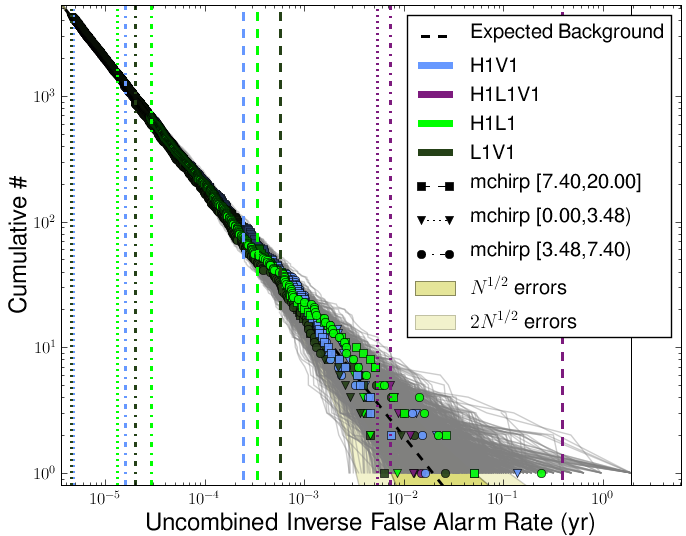
\includegraphics[width=4.5in]{figures/H1L1V1-ligolw_cbc_plotifar_FULL_DATA_CAT_4_VETO_cumhist_uncombined_ifar_ALL_DATA_PLOTTED_OPEN_BOX-931035296-4763191.png}}
\subfigure[Combined IFAR plot]{\label{fig:sample_plotifar_combined}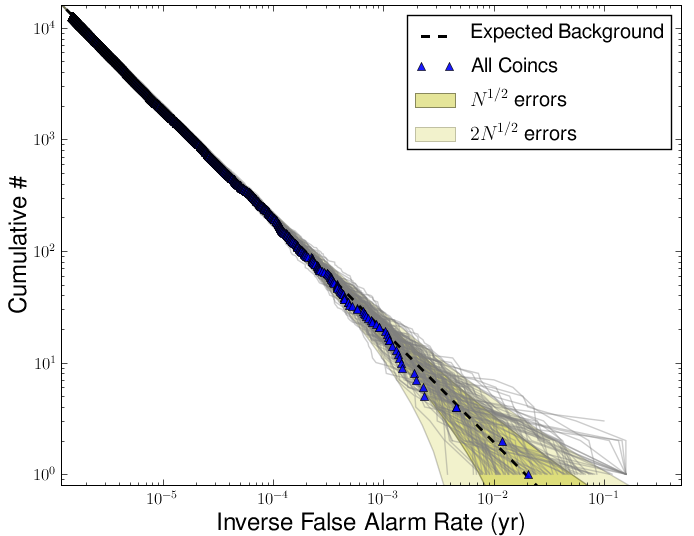
\includegraphics[width=4.5in]{figures/H1L1V1-ligolw_cbc_plotifar_FULL_DATA_CAT_4_VETO_cumhist_combined_ifar_ALL_DATA_PLOTTED_OPEN_BOX-931035296-4763191.png}}
\end{center}
\label{fig:sample_plotifar}
\caption{Sample IFAR plots created by \texttt{ligolw\_cbc\_plotifar}. Both plots taken from $\sim6$ weeks of \ac{S6} data, between GPS times 931035296 and 935798487. In both plots, the black dashed-line indicates the expected background distribution, yellow-shaded regions are the expected background $\pm \sqrt{N}$ and $\pm \sqrt{2N}$, and gray lines are slide distributions when treated as zero-lag. The blue triangles in the bottom plot indicate the zero-lag distribution of combined IFARs. The top plot shows the uncombined IFAR distribution, with each symbol representing a separate chirp-mass bin and each color a coincident \ac{IFO} combination. Colored dashed lines indicate maximum (minimum) background \ac{FAR} (IFAR).}
\end{figure}

\begin{figure}[p]
\label{fig:sample_plotcumhist}
\begin{center}
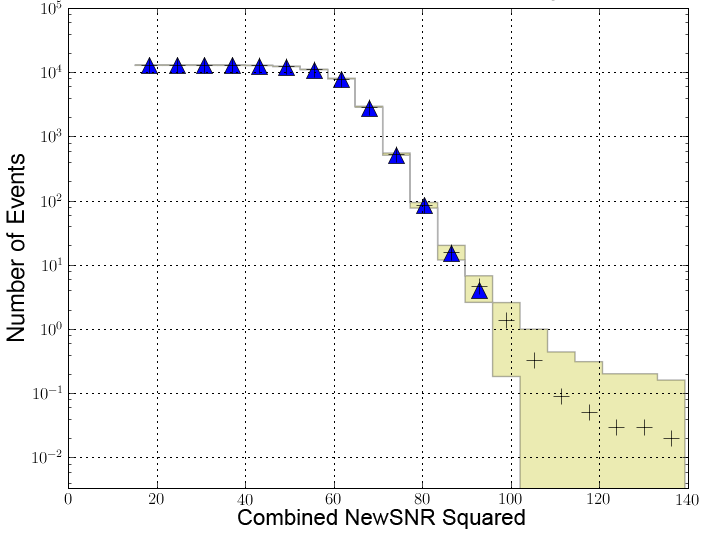
\includegraphics[width=5in]{figures/H1L1V1-ligolw_cbc_plotcumhist_FULL_DATA_CAT_4_VETO_cumhist_combined_snr_sq_ALL_DATA_PLOTTED_OPEN_BOX-931035296-4763191.png}
\end{center}
\caption{Sample cumulative histogram created by \texttt{ligolw\_cbc\_plotcumhist}. Data taken from $\sim6$ weeks of \ac{S6} data, between GPS times 931035296 and 935798487. Despite the label, \emph{new} \ac{SNR} squared is plotted on the x-axis (not \ac{SNR}). The data is binned and the cumulative number of triggers with new \ac{SNR} greater-than or equal-to a given bin are plotted on they y-axis. Zero-lag triggers are indicated by blue triangles. The mean slide counts are indicated by the black crosses and the shaded regions show the standard deviation across the slides.}
\end{figure}

\begin{figure}[p]
\begin{center}
\subfigure[Sample duration-per-slide plot for H1L1V1 time.]{\label{fig:sample_plotslide-H1L1V1_duration}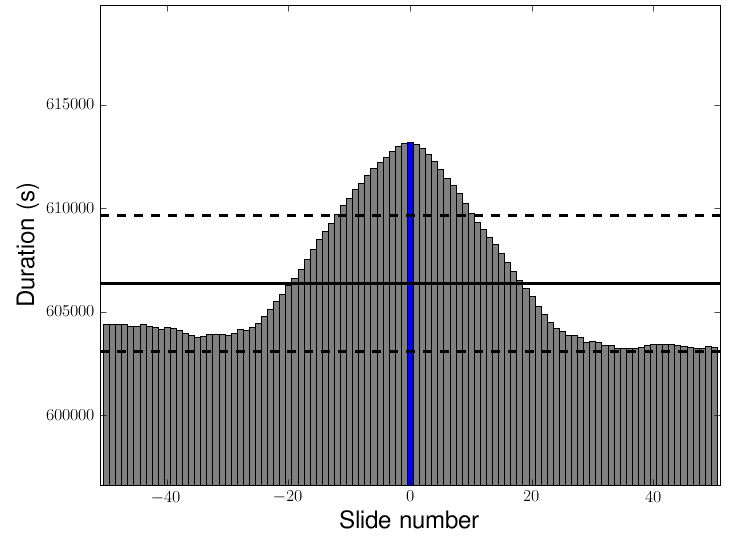
\includegraphics[width=4.5in]{figures/H1L1V1-ligolw_cbc_plotslides_FULL_DATA_CAT_4_VETO_durations_per_slide_ALL_DATA_PLOTTED-931035296-4763191.png}}
\subfigure[Sample duration-per-slide plot for H1L1 time.]{\label{fig:sample_plotslide-H1L1_duration}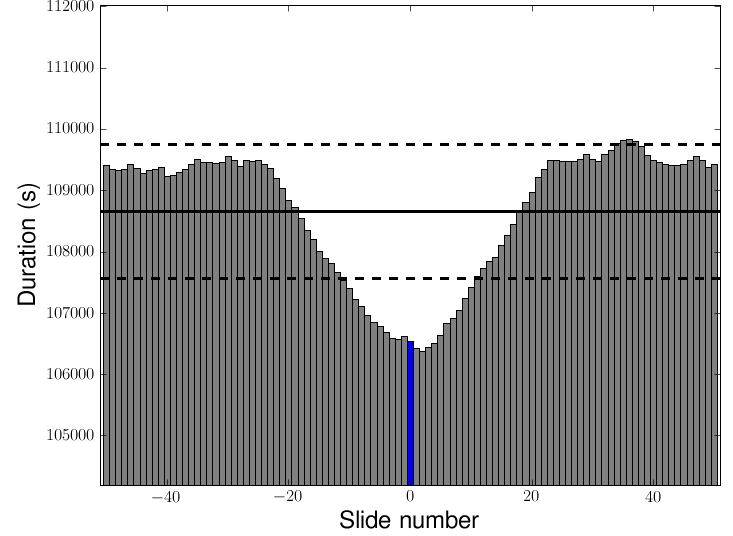
\includegraphics[width=4.5in]{figures/H1L1-ligolw_cbc_plotslides_FULL_DATA_CAT_4_VETO_durations_per_slide_ALL_DATA_PLOTTED-931035296-4763191.png}}
\end{center}
\label{fig:sample_plotslide-duration}
\caption{Sample duration-per-slide plots created by \texttt{ligolw\_cbc\_plotslides}. Both plots taken from $\sim6$ weeks of \ac{S6} data, between GPS times 931035296 and 935798487. The top plots shows the duration per slide for H1L1V1 time; the bottom, H1L1 time. These plots are after CAT3 (cumulative) vetoes have been applied. Gray bars show the duration in each slide; the blue bar shows the zero-lag duration. The black solid line is the mean duration and the dashed lines show the standard deviation.}
\end{figure}

\begin{figure}[p]
\label{fig:sample_plotslide-rate}
\begin{center}
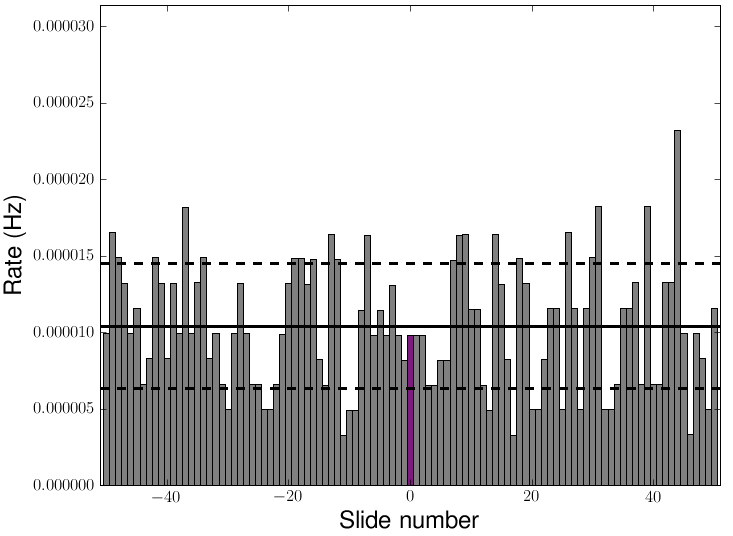
\includegraphics[width=5in]{figures/H1L1V1-ligolw_cbc_plotslides_FULL_DATA_CAT_4_VETO_H1L1V1_rates_ALL_DATA_PLOTTED_OPEN_BOX-931035296-4763191.png}
\end{center}
\caption{Sample trigger-rate-per-slide plot created by \texttt{ligolw\_cbc\_plotslides}. The data is from the same time as Figure \ref{fig:sample_plotslide-duration}. Shown is the rate of H1L1V1 triggers in H1L1V1 time in each slide. Gray bars indicate the rate in each slide; the purple bar shows the rate in zero-lag. (The color of the zero-lag bar is based on the coincident \acp{IFO}.) The black solid line shows the mean rate and the dashed lines the standard deviation.}
\end{figure}

\begin{figure}[p]
\label{fig:plotfm-dist_v_mchirp}
\begin{center}
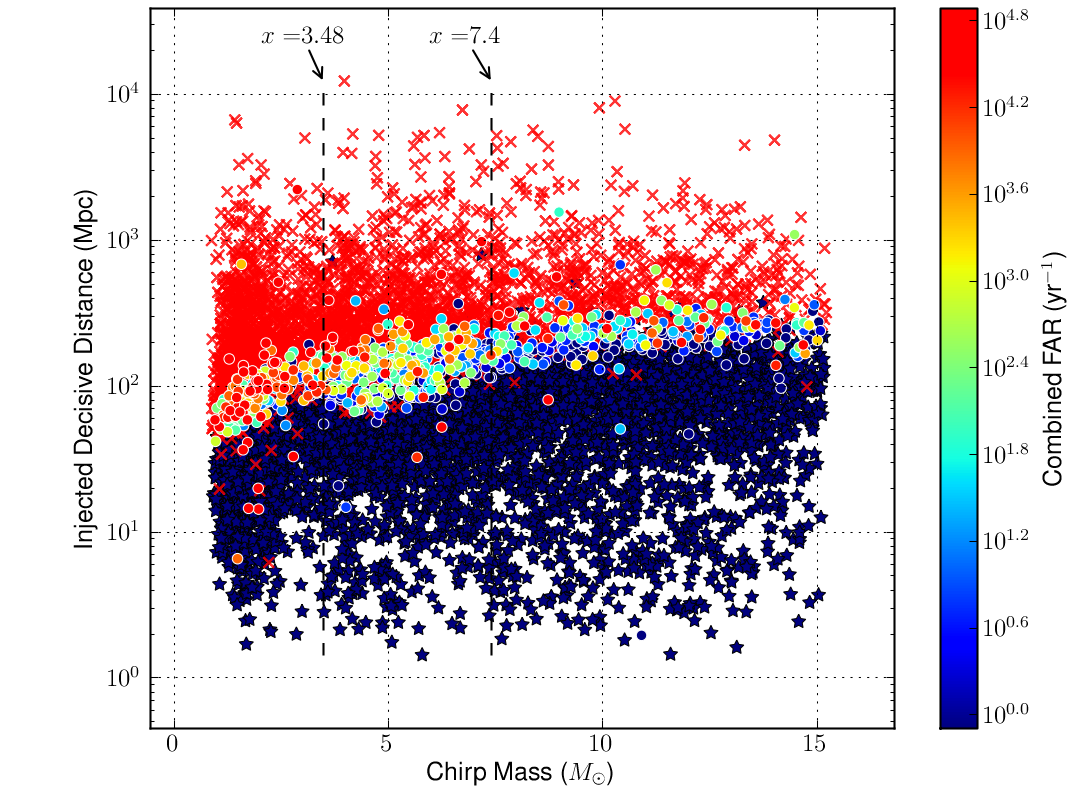
\includegraphics[width=6in]{figures/H1L1-ligolw_cbc_plotfm_fm_dist_v_param_ALLINJ_CAT_4_VETO_F1_ALLINJ_PLOTTED-956707143-4838544.png}
\end{center}
\caption{Sample decisive distance versus chirp mass plot for H1L1 time created by \texttt{ligolw\_cbc\_plotfm}. The data is taken from $\sim6$ weeks of \ac{S6} data, between GPS times 961545543 and 965174487. The blue stars are injections found with a combined \ac{FAR} equal to zero. The circles are injections found with non-zero combined \ac{FAR}; they are colored according to their combined \ac{FAR}. Missed injections are indicated by red crosses. The black dashed lines show the chirp mass boundaries used.}
\end{figure}

\begin{figure}[p]
\begin{center}
\subfigure[Chirp mass fractional difference versus end-time accuracy.]{\label{fig:plotfm-mchirp_frac_v_dt}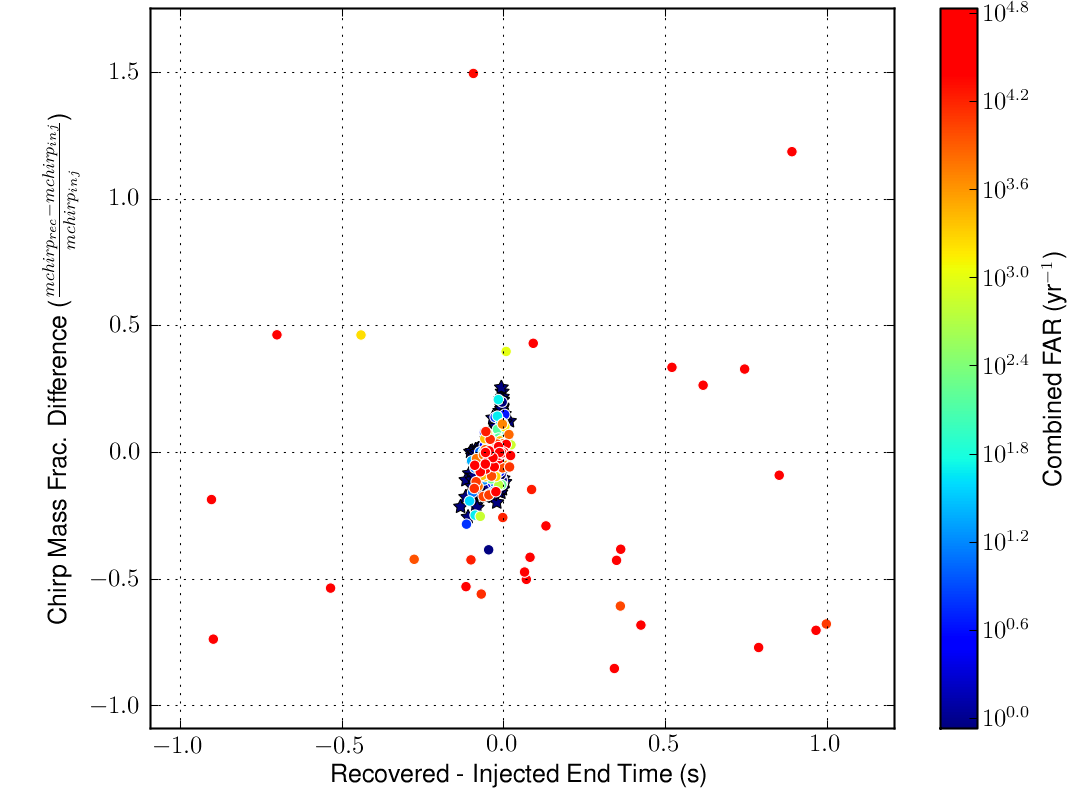
\includegraphics[width=5in]{figures/H1L1-ligolw_cbc_plotfm_fm_lin_plots_ALLINJ_CAT_4_VETO_F3_ALLINJ_PLOTTED-961545543-3628944.png}}
\subfigure[Injection type versus end-time accuracy.]{\label{fig:plotfm-injtag_v_dat}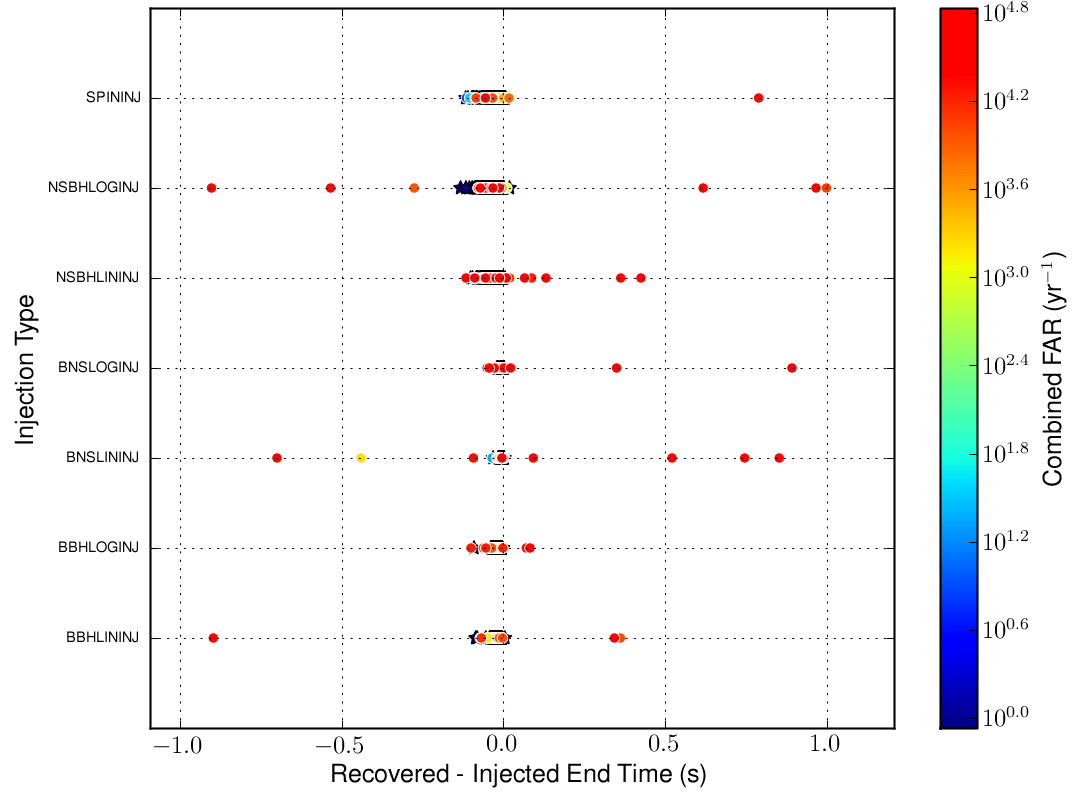
\includegraphics[width=5in]{figures/H1L1-ligolw_cbc_plotfm_fm_lin_plots_ALLINJ_CAT_4_VETO_F2_ALLINJ_PLOTTED-961545543-3628944.png}}
\end{center}
\label{fig:plotfm-example_v_dt}
\caption{More examples of PlotFM plots. The data used and color-coding is the same as in figure \ref{fig:plotfm-dist_v_mchirp}.}
\end{figure}

\clearpage

%\begin{table}[hp]
%\label{tab:sample-loudest_all_data_events}
%\begin{scriptsize}
%\center
%\begin{tabular}{| c | c | c | c | c | c | c | c | c | c | c | c | c |} 
%\hline
%\parbox[c]{1.1cm}{\center rank \\ (using \\ combined \\ far)} & \parbox[c]{1.1cm}{\centering combined \\ far} & fap & snr & end time & \parbox[c]{1.2cm}{\center end time utc} & ifos & mass & mchirp & \parbox[c]{1.1cm}{\centering mini \\ followup} & \parbox[c]{0.8cm}{\centering omega \\ scan} & \parbox[c]{1.1cm}{\centering all data \\ duration \\ (days)} \\
%\hline \hline
%1 & 0.0 & 0.0 & 22.29 & 962841819.07 & \parbox[c]{1.2cm}{\center Sun 11 \\ Jul 2010 \\ 00:03:24} & H1,L1 & 3.35 & 1.46 & link & H1 L1 & \\
%\cline{1-11}
%2 & 57.11 & 0.87 & 9.25 & 964110645.94 & \parbox[c]{1.2cm}{\center Sun 25 \\ Jul 2010 \\ 16:30:30} & H1,L1 & 20.95 & 3.34 & link & H1 L1 & \multirow{2}{*}{15.58} \\
%\cline{1-11}
%3 & 85.95 & 0.95 & 8.88 & 965116842.39 & \parbox[c]{1.3cm}{\center Fri 06 \\ Aug 2010 \\ 08:00:27} & H1,L1 & 12.29 & 4.32 & link & H1 L1 & \\
%\hline
%\end{tabular}
%\end{scriptsize}
%\end{table}

\begin{figure}[p]
\label{fig:example-loudest_all_data_events}
\center
\fbox{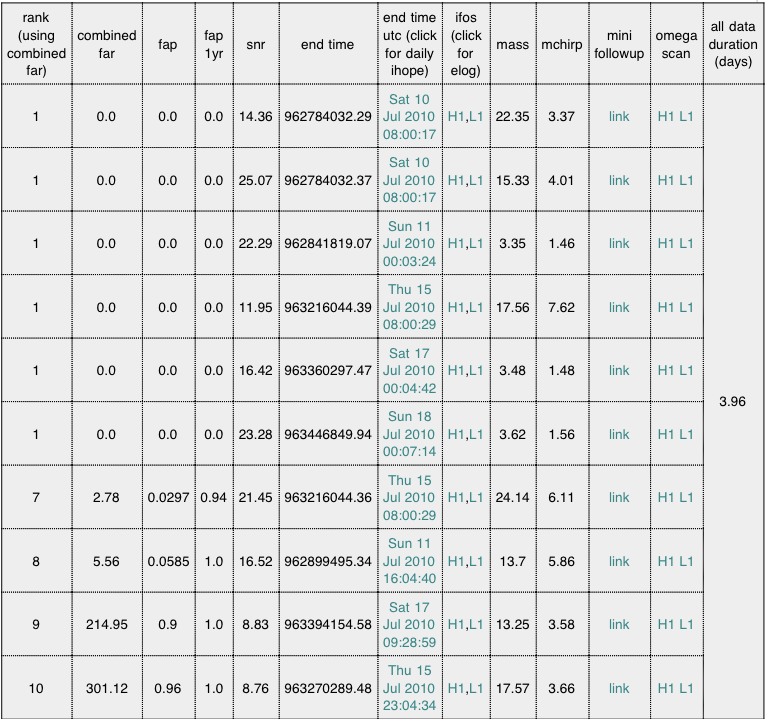
\includegraphics[width=6in]{figures/all_data-loudest_events/example-loudest_all_data_events.png}}
\caption{An example \texttt{all\_data} loudest-events list created by PrintLC when run in Pipedown.}
\end{figure}

\begin{figure}[p]
\begin{center}
\subfigure[A screen shot of the MiniFollowup page.]{\label{fig:sample-minifup_hardware_inj-screenshot}\fbox{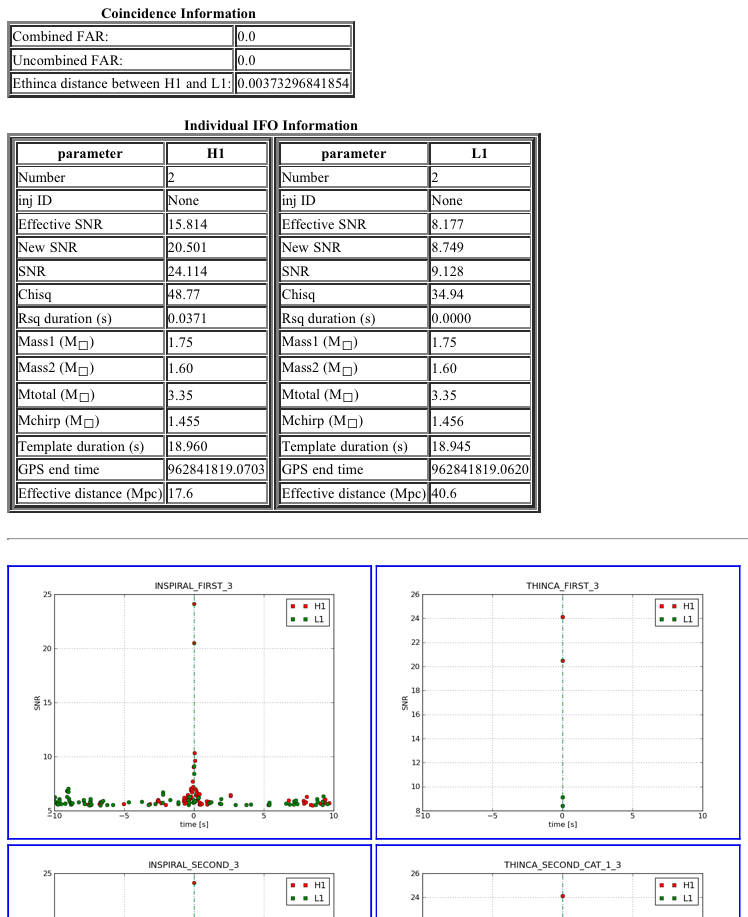
\includegraphics[height=3.8in]{figures/all_data-loudest_events/minifup-example_page.png}}}
\subfigure[A close-up of the \texttt{INSPIRAL\_FIRST} MiniFollowup plot.]{\label{fig:sample-minifup_hardware_inj-inspiral_first}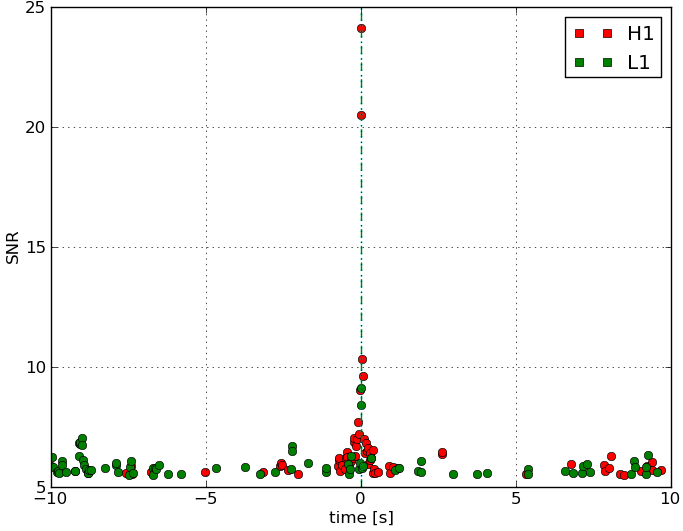
\includegraphics[width=4.8in]{figures/all_data-loudest_events/H1L1-FULL_DATA_CAT_2_VETO_FULL_DATA_map-INSPIRAL_FIRST-3_LOUDEST_ALL_DATA_EVENTS_BY_COMBINED_FAR_SUMMARY-962755143-1209744.png}}
\end{center}
\label{fig:sample-minifup_hardware_inj}
\caption{The MiniFollowup page for the third event, a hardware injection, in the loudest events list shown in Figure \ref{fig:example-loudest_all_data_events}. The top figure shows a screen shot of the page. The bottom figure shows \texttt{INSPIRAL\_FIRST} plot from that page.}
\end{figure}

\begin{figure}[p]
\center
\subfigure[The H1 Omega scan.]{\label{fig:sample-omega_hardware_inj-H1}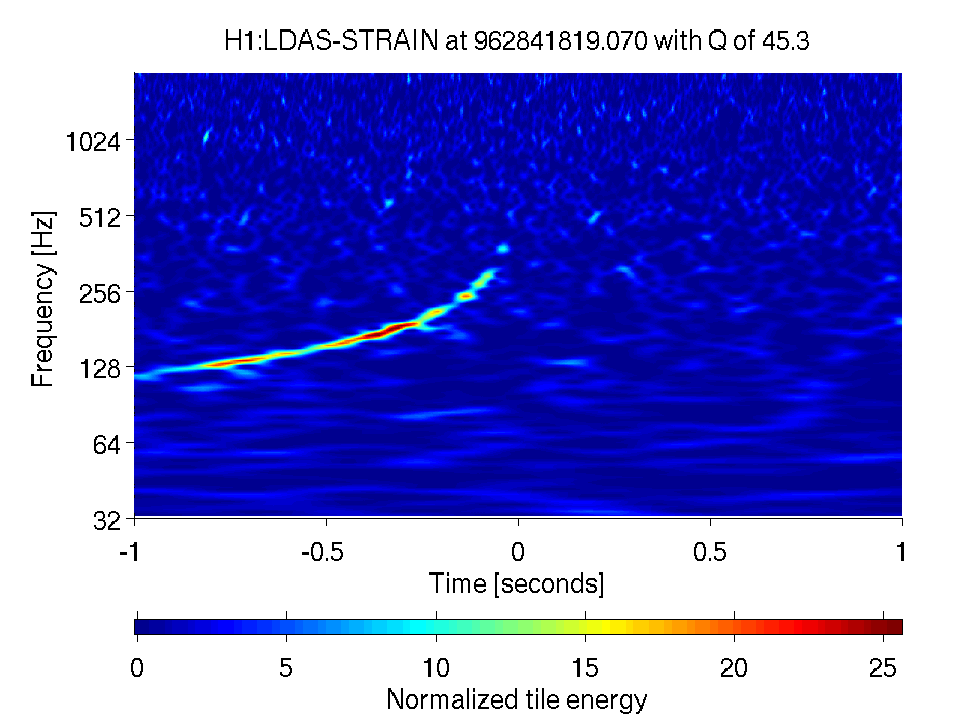
\includegraphics[width=5in]{figures/all_data-loudest_events/962841819_0703125_H1_LDAS-STRAIN_2_00_spectrogram_whitened.png}}
\subfigure[The L1 Omega scan.]{\label{fig:sample-omega_hardware_inj-L1}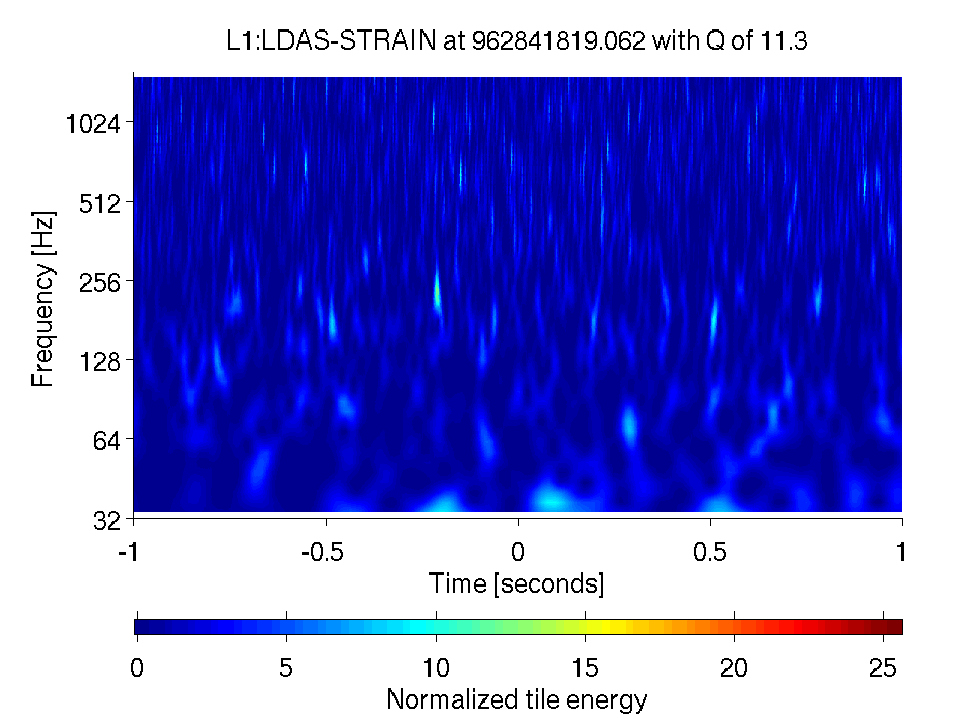
\includegraphics[width=5in]{figures/all_data-loudest_events/962841819_062011718_L1_LDAS-STRAIN_2_00_spectrogram_whitened.png}}
\label{fig:sample-omega_hardware_inj}
\caption{An example of an Omega scan. These scans are of the hardware injection shown in Figure \ref{fig:sample-minifup_hardware_inj}. The ``normalized tile energy'' is roughly equivalent to SNR$^2$/2 in a time-frequency tile. For Gaussian noise in the absence of signal, the normalized tile energy rarely exceeds 8. }
\end{figure}

\begin{figure}[p]
\label{fig:example-loudest_slide_events}
\center
\fbox{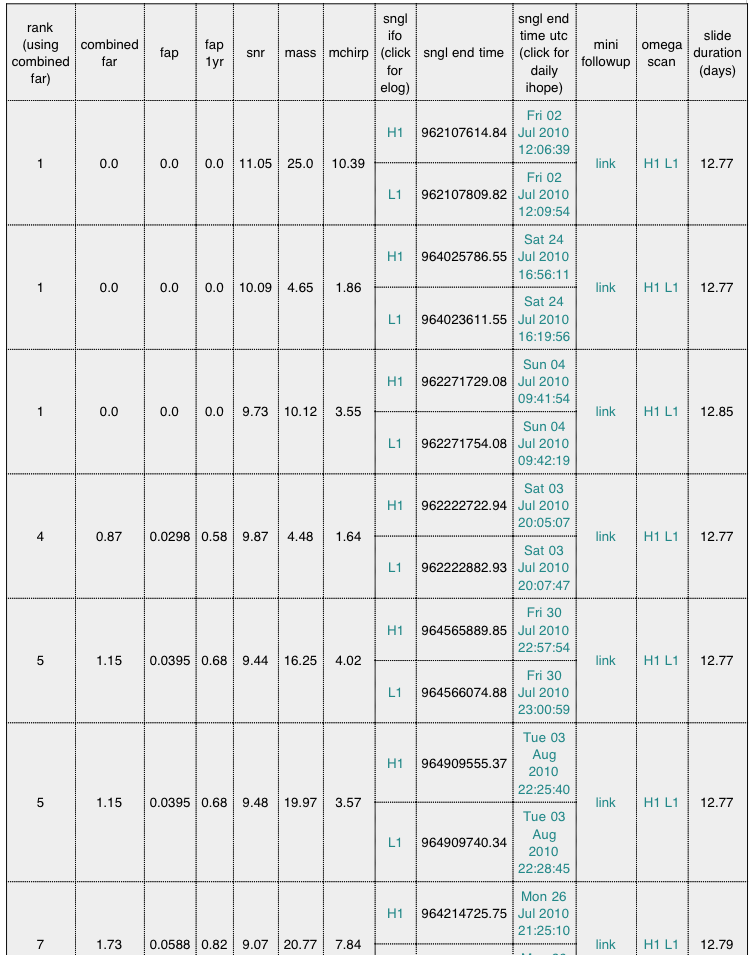
\includegraphics[width=6in]{figures/slide-loudest_events/example-loudest_slide_events.png}}
\caption{An example \texttt{slide} loudest-events list created by PrintLC when run in Pipedown.}
\end{figure}

\begin{figure}[p]
\begin{center}
\label{fig:sample-minifup_slide}
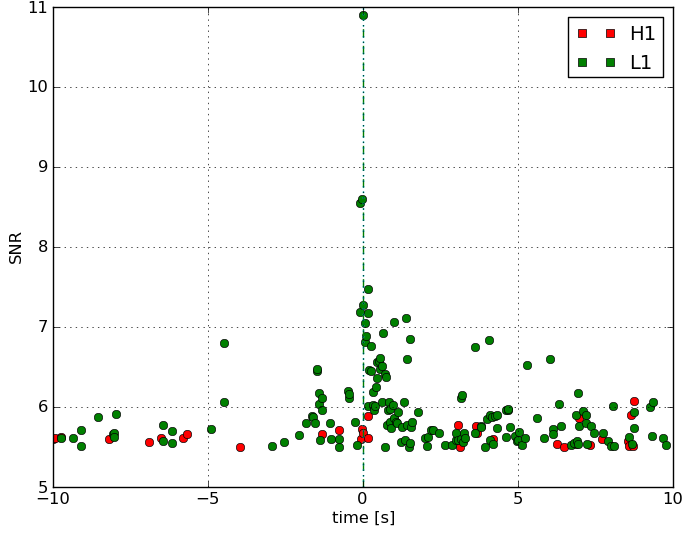
\includegraphics[width=4.8in]{figures/slide-loudest_events/H1L1-FULL_DATA_CAT_3_VETO_FULL_DATA_map-INSPIRAL_FIRST-3_LOUDEST_SLIDE_EVENTS_BY_COMBINED_FAR_SUMMARY-961545543-3628944.png}
\end{center}
\caption{The \texttt{INSPIRAL\_FIRST} mini-followup plot for the first loudest slide event (the one on Friday July 2 2010) shown in Figure \ref{fig:example-loudest_slide_events}.}
\end{figure}

\begin{figure}[p]
\center
\subfigure[The H1 Omega scan.]{\label{fig:sample-omega_slide-H1}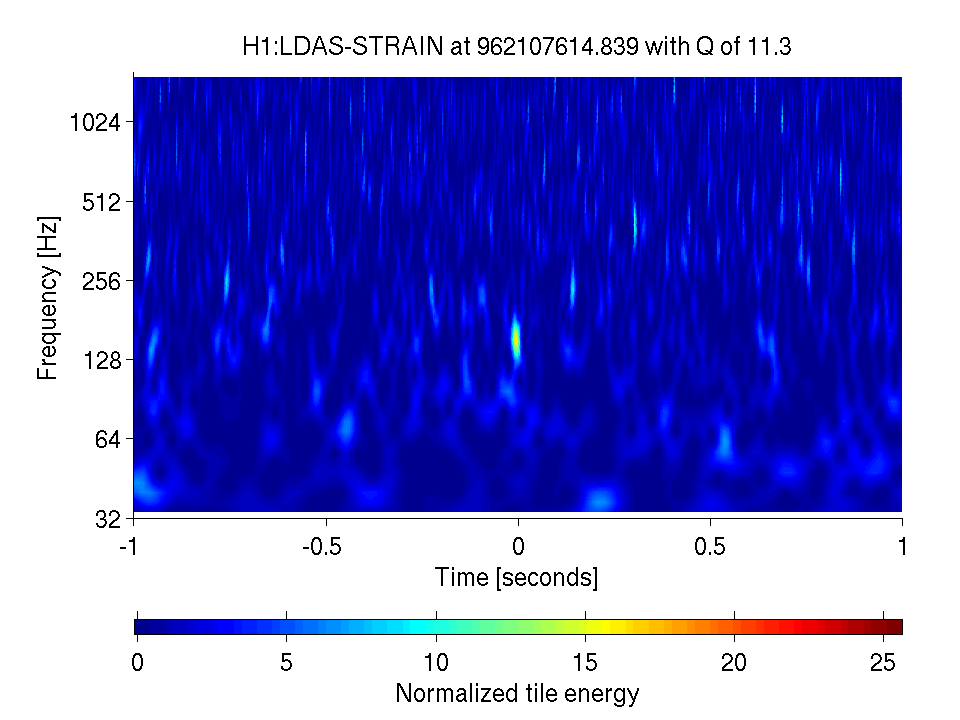
\includegraphics[width=5in]{figures/slide-loudest_events/962107614_839111328_H1_LDAS-STRAIN_2_00_spectrogram_whitened.png}}
\subfigure[The L1 Omega scan.]{\label{fig:sample-omega_slide-L1}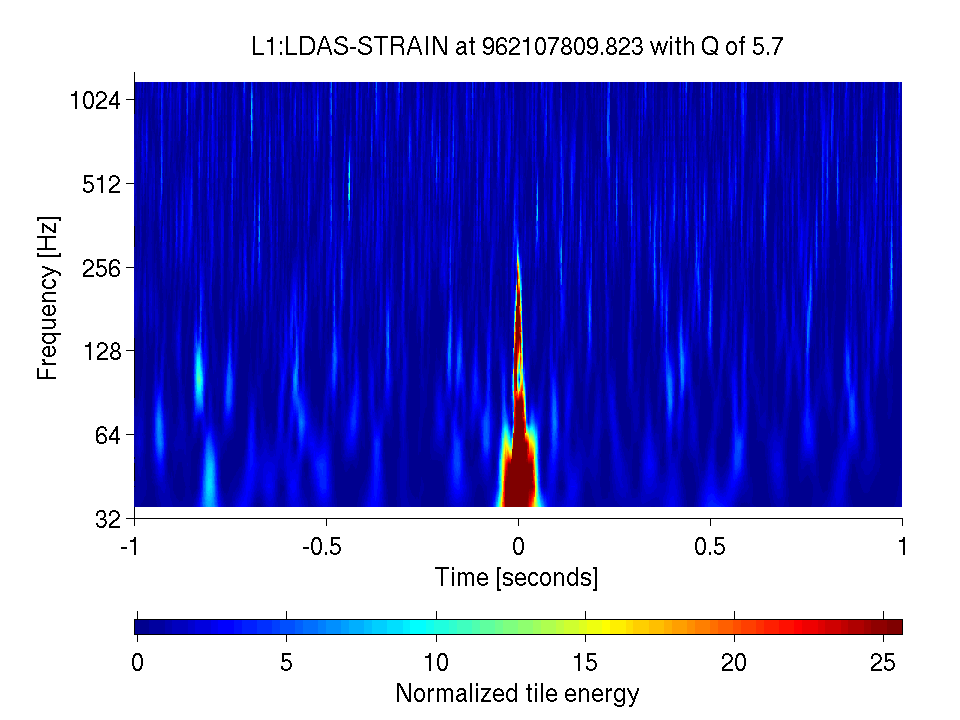
\includegraphics[width=5in]{figures/slide-loudest_events/962107809_823242187_L1_LDAS-STRAIN_2_00_spectrogram_whitened.png}}
\label{fig:sample-omega_slide}
\caption{The Omega scans of the slide event shown in Figure \ref{fig:sample-minifup_slide}.}
\end{figure}

\begin{figure}[p]
\label{fig:sample-daily_ihope-slide}
\begin{center}
\fbox{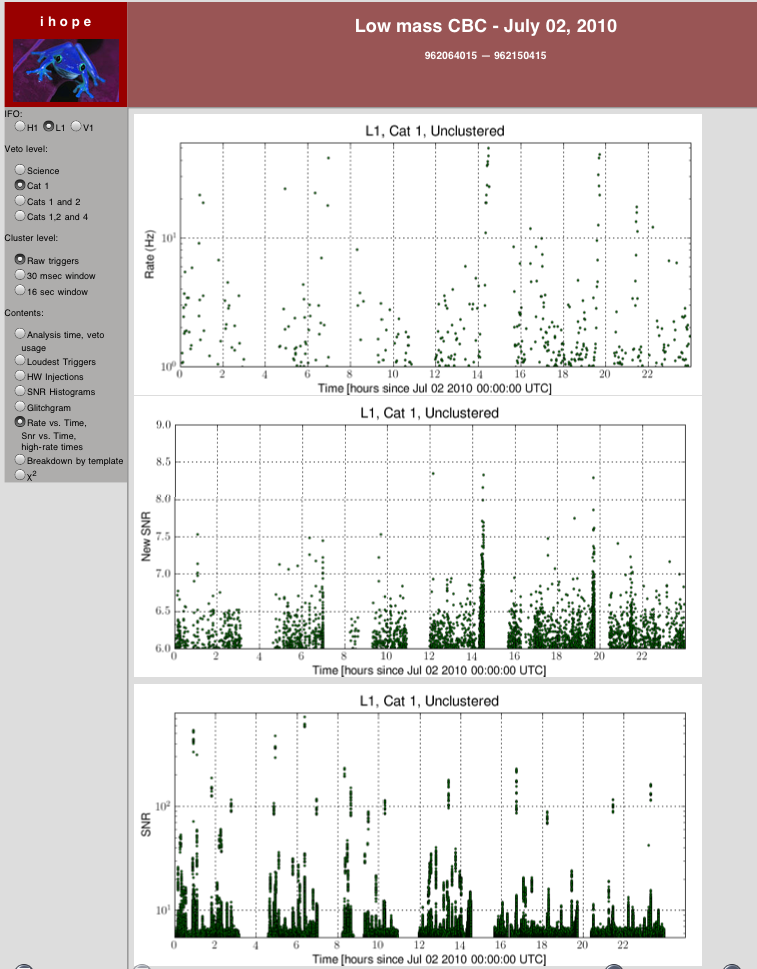
\includegraphics[height=7in]{figures/slide-loudest_events/example-daily_ihope_slide.png}}
\end{center}
\caption{A screen shot of a daily \ihope page. This page is from the same day as the loudest slide event shown in Figures \ref{fig:sample-minifup_slide} and \ref{fig:sample-omega_slide}. It can be accessed from the loudest-events table by clicking on the \texttt{sngl end time utc} for the trigger. Shown is the rate, new \ac{SNR} and \ac{SNR} of triggers as a function of time for L1 after CAT1 vetoes have been applied. As evident from the side bar, there are several other plots and lists available for all the \acp{IFO} at various vetoes and clustering windows. For more details on daily \ihope see \cite{ref:Larne}.}
\end{figure}

\begin{figure}[p]
\label{fig:sample-elog-slide}
\begin{center}
\fbox{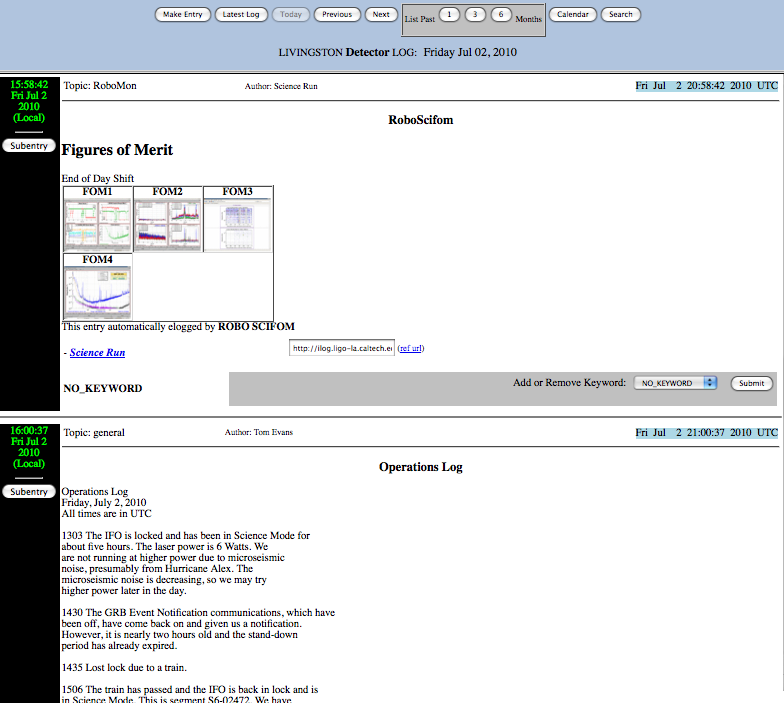
\includegraphics[width=6in]{figures/slide-loudest_events/sample-elog.png}}
\end{center}
\caption{A screen shot of a L1 e-log. The day shown is from the same day as the loudest slide event shown in Figures \ref{fig:sample-minifup_slide} and \ref{fig:sample-omega_slide}. It can be accessed from the loudest-events table by clicking on the ``L1" in the \texttt{sngl ifo} column for the trigger.}
\end{figure}

\begin{figure}[p]
\center
\subfigure[All injections.]{\label{fig:sample-printmissed_ALLINJ}\fbox{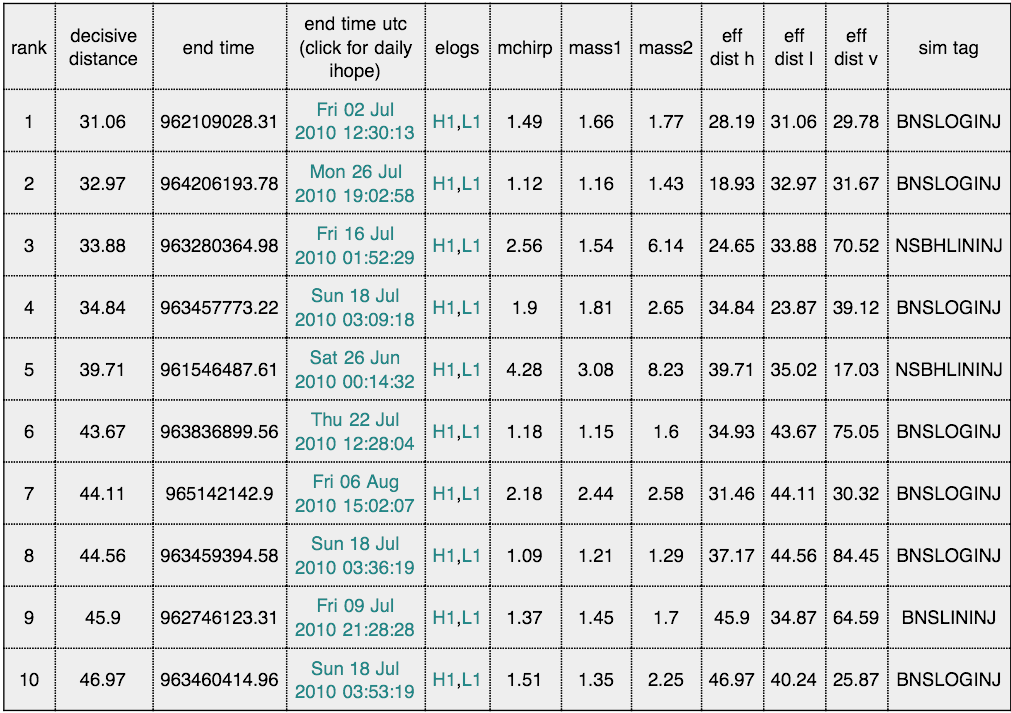
\includegraphics[width=6in]{figures/missed_injection-example/example-printmissed_ALLINJ.png}}}
\subfigure[The \texttt{BNSLOGINJ} table.]{\label{fig:sample-printmissed_BNSLOGINJ}\fbox{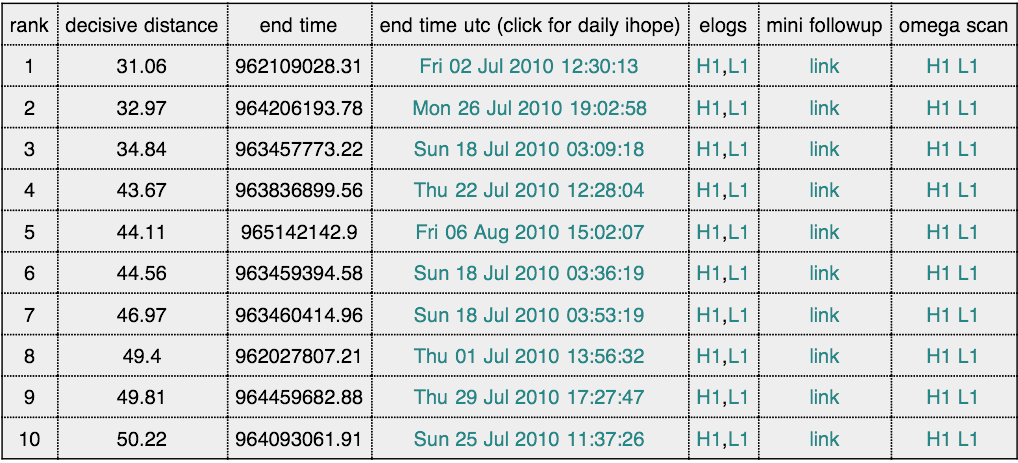
\includegraphics[width=6in]{figures/missed_injection-example/example-printmissed_BNSLOGINJ.png}}}
\label{fig:sample-printmissed}
\caption{Example tables produced by PrintMissed when run in Pipedown. The top table shows the 10 closest missed injections out of all of the injection runs. The bottom table shows the 10 closest missed injections in the \texttt{BNSLOGINJ} run. Note that in the second table, mini-followup and Omega scan links have been added.}
\end{figure}

\begin{figure}[p]
\center
\subfigure[A screen shot of the found/missed table produced by MiniFollowups.]{\label{fig:sample-minifup_missedinj-table}\fbox{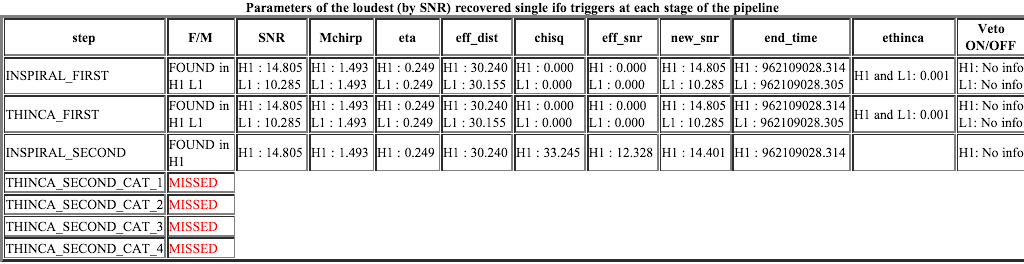
\includegraphics[width=6in]{figures/missed_injection-example/example-missedinj_minifup.png}}}
\subfigure[The \texttt{INSPIRAL\_FIRST} plot from the mini-followup page for this missed injection.]{\label{fig:sample-minifup_missedinj-plot}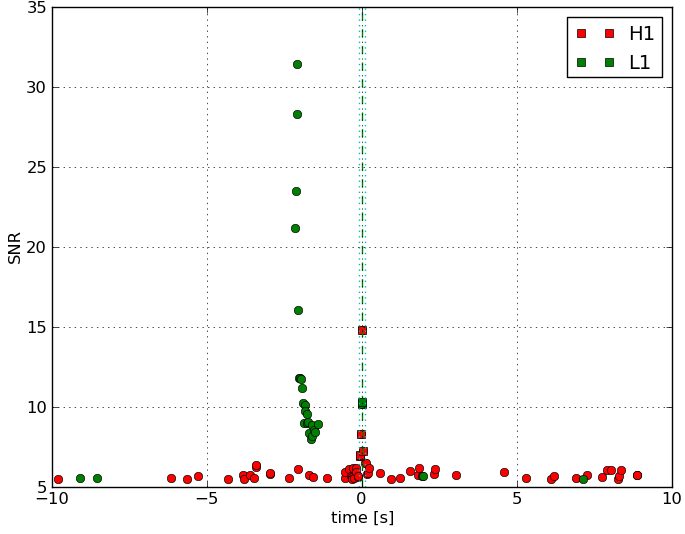
\includegraphics[width=5in]{figures/missed_injection-example/H1L1-BNSLOGINJ_CAT_4_VETO_BNSLOGINJ_map-INSPIRAL_FIRST-1_CLOSEST_MISSED_INJECTIONS_SUMMARY-961545543-3628944.png}}
\label{fig:sample-minifup_missedinj}
\caption{An example of the output produced by MiniFollowups when run on a missed injection. The top figure is a screen shot of the found/missed table that traces whether or not the injection was found, and with what parameters, at each stage in the pipeline. The bottom figure shows the \texttt{INSPIRAL\_FIRST} plot. This followup is for the closest missed injection shown in the tables shown in Figure \ref{fig:sample-printmissed}.}
\end{figure}

\begin{figure}[p]
\center
\subfigure[The H1 Omega scan.]{\label{fig:sample-omega_missedinj-H1}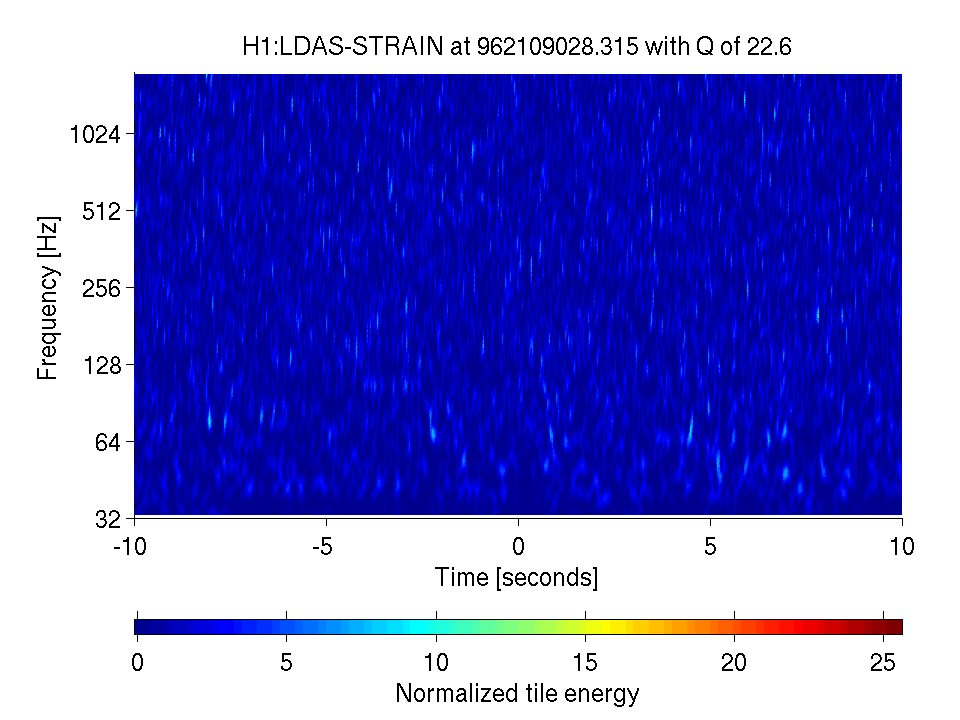
\includegraphics[width=5in]{figures/missed_injection-example/962109028_314747572_H1_LDAS-STRAIN_20_00_spectrogram_whitened.png}}
\subfigure[The L1 Omega scan.]{\label{fig:sample-omega_missedinj-L1}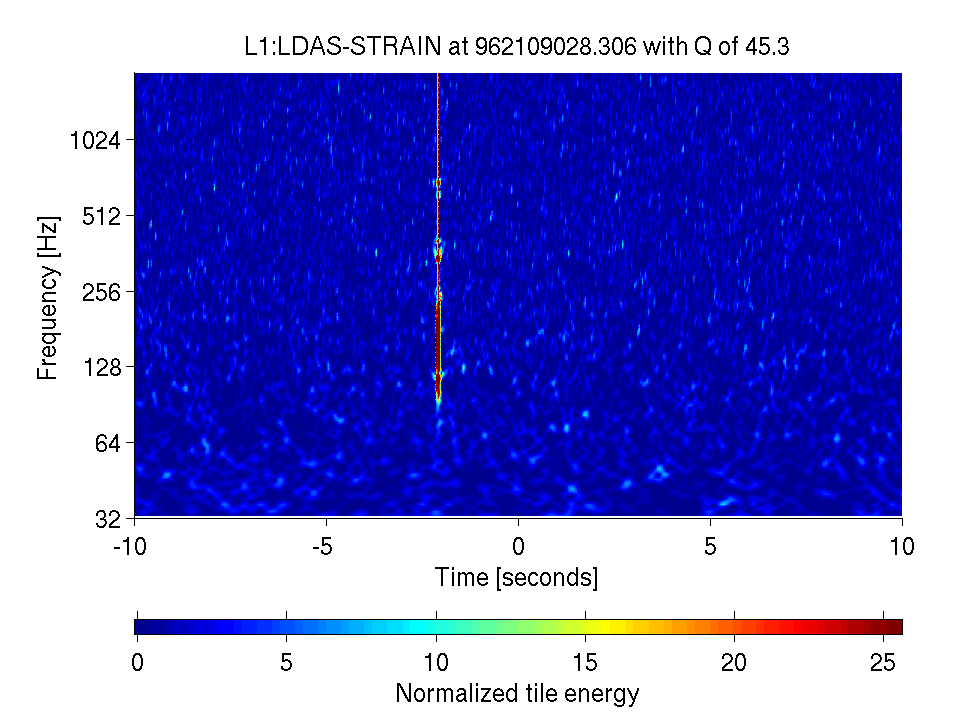
\includegraphics[width=5in]{figures/missed_injection-example/962109028_306081057_L1_LDAS-STRAIN_20_00_spectrogram_whitened.png}}
\label{fig:sample-omega_missedinj}
\caption{The Omega scans of the missed \texttt{BNSLOGINJ} injection detailed in Figure \ref{fig:sample-minifup_missedinj}. The H1 scan is clean, but the L1 scan shows a short-duration broadband glitch $\sim2\,$s before the injection's end time (which is placed at $0\,$s on the spectrograms). The H1 (and possibly the L1) \ac{SNR} of the injection is large enough to be seen in Omega scan. Nothing is seen because Omega scans do not currenlty show software injections.}
\end{figure}

\begin{figure}[p]
\center
\subfigure[All injections.]{\label{fig:sample-printsims_ALLINJ}\fbox{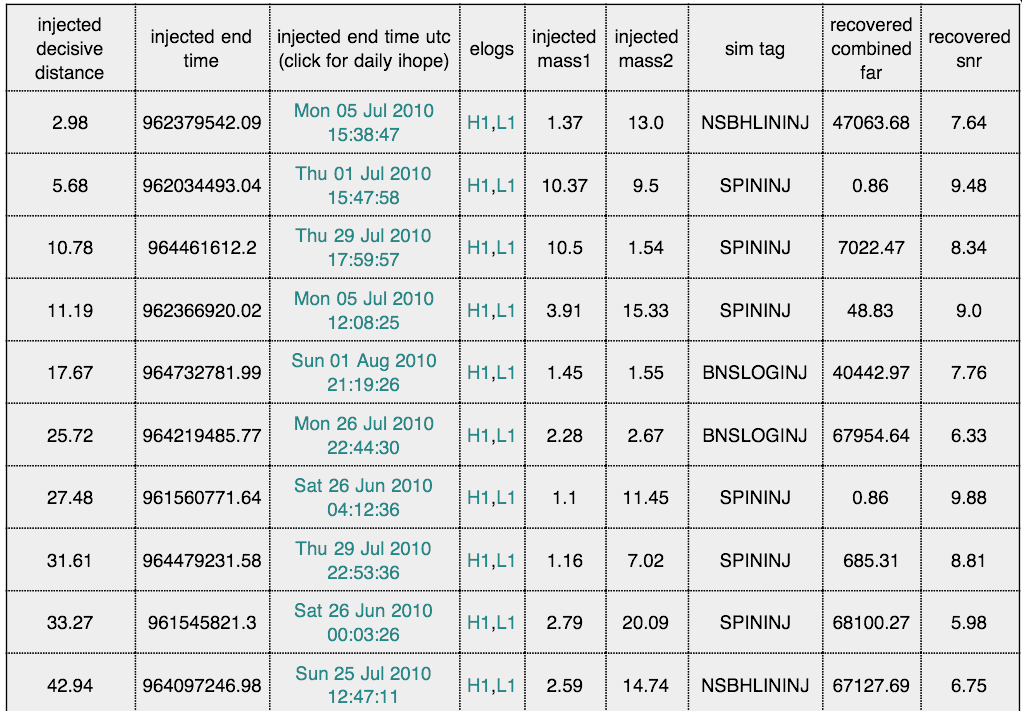
\includegraphics[width=5in]{figures/example-printsims_ALLINJ.png}}}
\subfigure[The \texttt{BNSLOGINJ} table.]{\label{fig:sample-printsims_BNSLOGINJ}\fbox{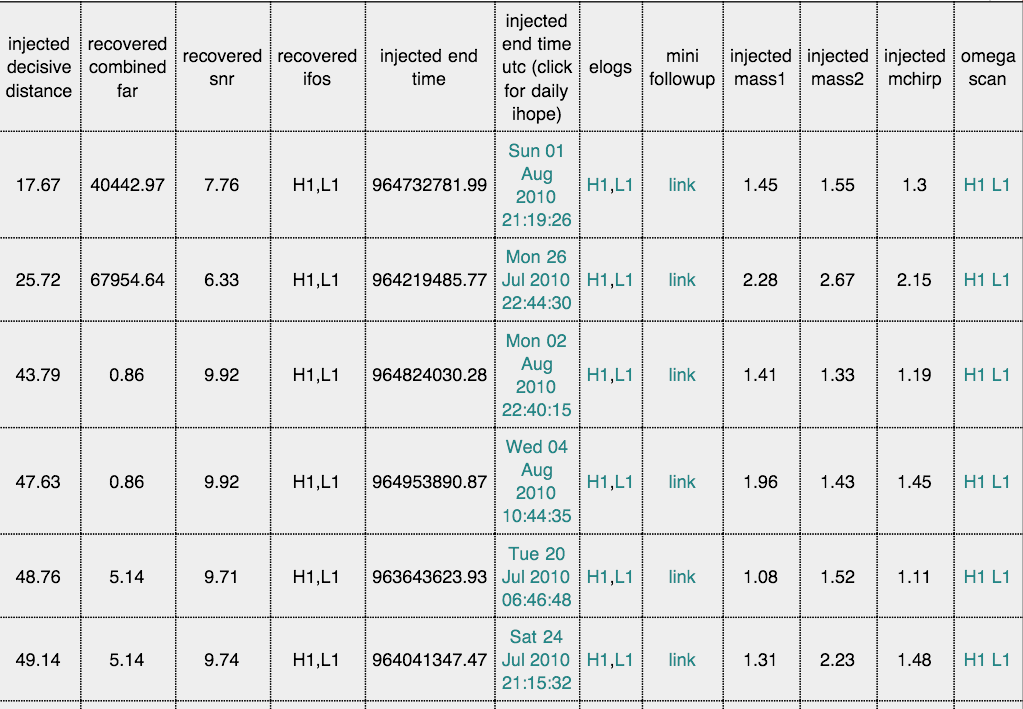
\includegraphics[width=5in]{figures/example-printsims_BNSLOGINJ.png}}}
\label{fig:sample-printsims}
\caption{An example of the tables produced by PrintSims when run in Pipedown. The top table shows a portion of the quiestest found table for all the injection runs. The bottom table shows a portion of \texttt{BNSLOGINJ} table. Note that in the latter table, mini-followup and Omega scan links have been added.}
\end{figure}

\clearpage

\section{Tying it All Together: The \ihope Page}
\label{sec:ihope_page}

The completion of all of the MiniFollowup jobs marks the end of Pipedown, and therefore the end of the \ihope pipeline. By this point we have many files and plots containing a wealth of information sprawled across the \ihope directory. To bring all of these files together into one easy-accessible place, we run \verb|write_ihope_page|. This program copies the most useful plots and files to a directory that's accessible to all \ac{LSC} and Virgo members through the internet. It then generates a web page that displays the plots and tables in clickable menus. Figure \ref{fig:sample_ihope_page} shows a screen shot of one of these \ihope pages. Shown is the IFAR plot with hardware injections left in the data (note the arrow on the loudest zero-lag triggers, indicating they have zero \acp{FAR}) and the corresponding PrintLC table. Clicking on the links in the table will open up the other pages, such as the MiniFollowup page and the Omega scans. Note that this is only one subsection; the right menu bar provides links to many other sections summarizing playground data, all injection runs (which includes the PlotFM plots discussed above, along with the PrintMissed and PrintSims tables), and other auxillarily information about the run.

The page shown in Figure \ref{fig:sample_ihope_page} is an open-box page. When we do a \ac{CBC} search, a closed-box \ihope page is initially generated. The format of the page is the same, but only plots and tables containing playground data are shown; \verb|all_data| information is off-limits (and the frog is not coming out of a box). Using this page, we check and followup the loudest slide triggers, as well as the missed and quietest found injections. If a new glitch class is found for which a cause can be determined, we create a veto for it (this would be a CAT2 or higher veto). We then re-run the \verb|THINCA_SECOND| stage and Pipedown, applying the new vetoes. The new closed box page is checked and, if everything looks good, an open-box page is generated. We then look at this page to see if we have found any gravitational waves.

Pipedown and the \ihope page, in the current form described here, were not developed until after \ac{S6} had started. Prior to this, and for \ac{S5}, scripts were run by hand to do the equivalent steps. However, the results were not as easily accessible, and so this method of checking loudest slide triggers to develop vetoes was not implemented until after Pipedown was completed, in the latter-half of \ac{S6}. In Chapter \ref{ch:s6_results} we detail some of the vetoes and tuning decisions that were made as a result of these loudest slide studies.

\begin{figure}
\label{fig:sample_ihope_page}
\begin{center}
\fbox{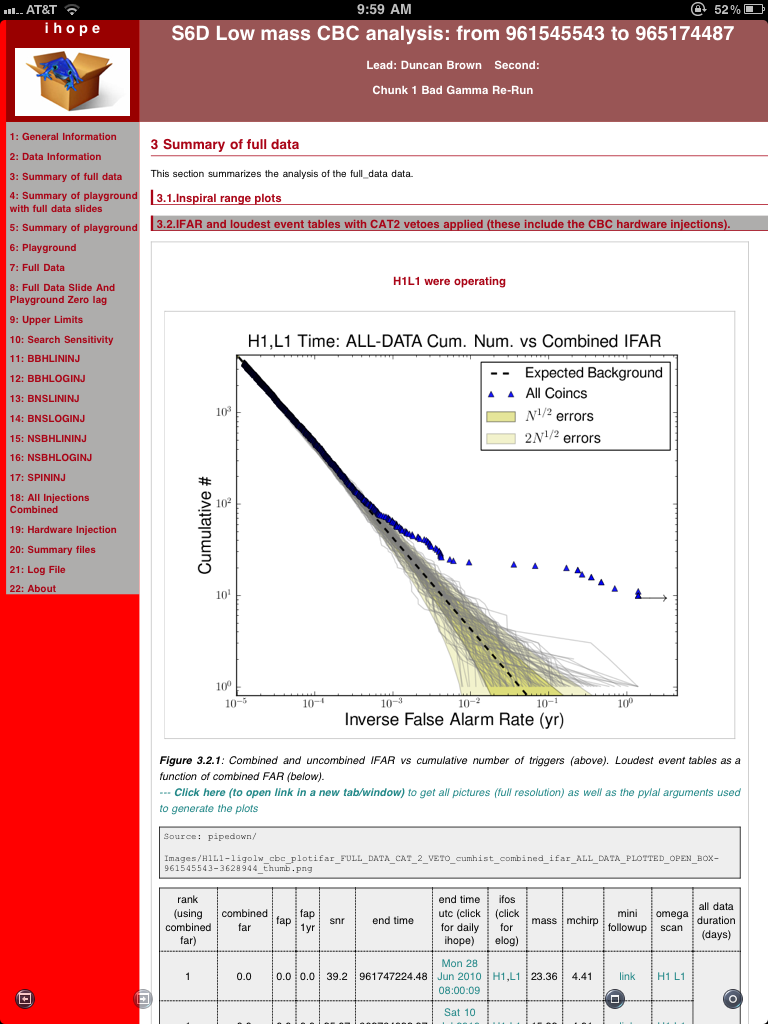
\includegraphics[height=7in]{figures/IhopePage-example.png}}
\end{center}
\caption{A screen shot of an \ihope page.}
\end{figure}


\Chapter{S5 Results}
\label{ch:s5_results}
\textit{\ac{S5} was broken up into three analysis periods by the \ac{CBC} group: the first calendar year, the 12--18 month search, and the LV search. The results from each of these analyses were published in Physical Review D. Below is a copy of the 12--18 month paper, which appeared in Phys. Rev. D90, 2009 047101. For the first year paper and the LV paper, see \cite{ref:s51yr} and \cite{ref:s5lvc}, respectively.}

%input{uls.tex} % run paper_uls.py in the scripts directory to update uls.tex
% non-spinning
\def\BNSul{\ensuremath{1.4 \times 10^{-2}}}
\def\NSBHul{\ensuremath{3.6 \times 10^{-3}}}
\def\BBHul{\ensuremath{7.3 \times 10^{-4}}}

% spinning
\def\SNSBHul{\ensuremath{4.4 \times 10^{-3}}}
\def\SBBHul{\ensuremath{9.0 \times 10^{-4}}}

% BNS NUMBERS
%%%%%%%%%%%%%%%%%%%%%%%%%%%%%%%%%%%%%%%
\def\BNStripleCumLum{\ensuremath{490}}
\def\BNSHoneLoneCumLum{\ensuremath{410}}
\def\BNSHtwoLoneCumLum{\ensuremath{110}}

\def\BNStripleCalErr{\ensuremath{23\%}}
\def\BNSHoneLoneCalErr{\ensuremath{23\%}}
\def\BNSHtwoLoneCalErr{\ensuremath{26\%}}

\def\BNStripleMonErr{\ensuremath{3\%}}
\def\BNSHoneLoneMonErr{\ensuremath{7\%}}
\def\BNSHtwoLoneMonErr{\ensuremath{10\%}}

\def\BNStripleWavErr{\ensuremath{31\%}}
\def\BNSHoneLoneWavErr{\ensuremath{32\%}}
\def\BNSHtwoLoneWavErr{\ensuremath{31\%}}

\def\BNStripleGDErr{\ensuremath{16\%}}
\def\BNSHoneLoneGDErr{\ensuremath{16\%}}
\def\BNSHtwoLoneGDErr{\ensuremath{3\%}}

\def\BNStripleGMErr{\ensuremath{19\%}}
\def\BNSHoneLoneGMErr{\ensuremath{19\%}}
\def\BNSHtwoLoneGMErr{\ensuremath{17\%}}
%%%%%%%%%%%%%%%%%%%%%%%%%%%%%%%%%%%%%%%

% BBH NUMBERS
%%%%%%%%%%%%%%%%%%%%%%%%%%%%%%%%%%%%%%%
\def\BBHtripleCumLum{\ensuremath{11000}}
\def\BBHHoneLoneCumLum{\ensuremath{9400}}
\def\BBHHtwoLoneCumLum{\ensuremath{2200}}

\def\BBHtripleCalErr{\ensuremath{25\%}}
\def\BBHHoneLoneCalErr{\ensuremath{24\%}}
\def\BBHHtwoLoneCalErr{\ensuremath{31\%}}

\def\BBHtripleMonErr{\ensuremath{3\%}}
\def\BBHHoneLoneMonErr{\ensuremath{7\%}}
\def\BBHHtwoLoneMonErr{\ensuremath{10\%}}

\def\BBHtripleWavErr{\ensuremath{33\%}}
\def\BBHHoneLoneWavErr{\ensuremath{34\%}}
\def\BBHHtwoLoneWavErr{\ensuremath{38\%}}

\def\BBHtripleGDErr{\ensuremath{13\%}}
\def\BBHHoneLoneGDErr{\ensuremath{15\%}}
\def\BBHHtwoLoneGDErr{\ensuremath{15\%}}

\def\BBHtripleGMErr{\ensuremath{16\%}}
\def\BBHHoneLoneGMErr{\ensuremath{17\%}}
\def\BBHHtwoLoneGMErr{\ensuremath{18\%}}
%%%%%%%%%%%%%%%%%%%%%%%%%%%%%%%%%%%%%%%

% NSBH NUMBERS
%%%%%%%%%%%%%%%%%%%%%%%%%%%%%%%%%%%%%%%
\def\NSBHtripleCumLum{\ensuremath{2000}}
\def\NSBHHoneLoneCumLum{\ensuremath{1700}}
\def\NSBHHtwoLoneCumLum{\ensuremath{453}}

\def\NSBHtripleCalErr{\ensuremath{24\%}}
\def\NSBHHoneLoneCalErr{\ensuremath{22\%}}
\def\NSBHHtwoLoneCalErr{\ensuremath{30\%}}

\def\NSBHtripleMonErr{\ensuremath{3\%}}
\def\NSBHHoneLoneMonErr{\ensuremath{7\%}}
\def\NSBHHtwoLoneMonErr{\ensuremath{10\%}}

\def\NSBHtripleWavErr{\ensuremath{32\%}}
\def\NSBHHoneLoneWavErr{\ensuremath{32\%}}
\def\NSBHHtwoLoneWavErr{\ensuremath{36\%}}

\def\NSBHtripleGDErr{\ensuremath{13\%}}
\def\NSBHHoneLoneGDErr{\ensuremath{13\%}}
\def\NSBHHtwoLoneGDErr{\ensuremath{18\%}}

\def\NSBHtripleGMErr{\ensuremath{18\%}}
\def\NSBHHoneLoneGMErr{\ensuremath{19\%}}
\def\NSBHHtwoLoneGMErr{\ensuremath{19\%}}
%%%%%%%%%%%%%%%%%%%%%%%%%%%%%%%%%%%%%%%


\section{Introduction}\label{sec:overview}

In November 2005 the three first-generation detectors of the \ac{LIGO} reached
design sensitivity and began a two-year period of observations (known as the
fifth science run, or S5) which concluded in October 
2007~\cite{abbott:2007kva}.  One of the most promising sources of 
gravitational-waves for LIGO is a \ac{CBC}; the inspiral and merger of 
\ac{BNS}, \ac{BBH}, or a \ac{NSBH}~\cite{LIGOS1iul,LIGOS2iul,LIGOS2macho,
LIGOS2bbh,LIGOS3S4all,Collaboration:2009tt}. These systems spiral together as
they emit energy in the form of gravitational waves, finally merging to form a 
single object, which then settles down to equilibrium. Ground-based 
gravitational-wave detectors are most sensitive to waves with frequencies 
between $\sim 40$ and $1000$~Hz, corresponding to the late stages of inspiral 
and merger. In this paper we report the results of search for 
gravitational-waves from binaries with total mass between $2$ and $35~\Msun$ 
and a minimum component mass of $1~\Msun$ in LIGO observations between November 
14, 2006 and May 18, 2007. The results of a search for these systems in data 
taken from November 4, 2005 to November 14, 2006 were reported in 
Ref.~\cite{Collaboration:2009tt}. From May--October 2007, the Virgo 
gravitational-wave detector operated in coincidence with the \ac{LIGO} 
detectors~\cite{0264-9381-23-19-S01} and the \ac{LIGO} data from that period 
are being analyzed together with the Virgo data. The joint analysis requires 
significant modifications to our analysis pipeline: therefore results of that 
search will be reported in a subsequent publication. In contrast, the results 
presented here were obtained with substantially the same analysis pipeline used 
in Ref.~\cite{Collaboration:2009tt}.  

No gravitational-wave signals were observed during this search and so we
report upper limits on CBC rates using the upper limits of 
Ref.~\cite{Collaboration:2009tt} as prior rate distributions. We summarize the 
analysis procedure and we present the search results and upper limits on CBC 
rates derived from \ac{LIGO} observations in the period November 4, 2005 to May
18, 2007.

%%%%%%%%%%%%%%%%%%%%%%%%%%%%%%%%%%%%%%%
\section{The Data analysis pipeline}
\label{sec:pipeline}

The data-analysis pipeline used in this search is fundamentally the same as
that of Ref.~\cite{Collaboration:2009tt}, thus here we only describe the major 
components and highlight differences to the previous search, referring to 
Refs.~\cite{LIGOS3S4all,Collaboration:2009tt} for details. The most substantial
change in this analysis is a modification to the way in which the significance
of candidate events is compared to instrumental noise background. In previous
searches, the noise background was computed \emph{using the entire observation
period} by introducing an artificial time shift between data recorded at the
two LIGO observatories. The observation period is split into six four-week 
segments and one 18 day segment (referred to as ``months'') and the 
instrumental background is measured \emph{independently in each month}, as the
detector behavior varied over the course of the S5 run. Candidate triggers are
therefore compared to a background that better reflects the instrumental 
behavior at the time of the candidate.  Each month was searched independently 
for gravitational-wave candidates and in the absence of detections, the results
from the months are combined (together with the results from
Ref.~\cite{Collaboration:2009tt}) to set an upper limit on the CBC rate.

We search for gravitational-wave signals when at least two of the \ac{LIGO}
detectors were operational.  This comprised a total of $0.28$~yr when all three
detectors (the 4 and 2~km Hanford detectors, denoted H1 and H2, respectively, 
and the 4~km Livingston detector, denoted L1) were operational 
(H1H2L1 coincident data), $0.10$~yr of H1H2 coincident data, $0.02$~yr of H1L1 
coincident data, and $0.01$~yr of H2L1 coincident data.  Noise correlations 
between the colocated H1 and H2 detectors cause our method of estimating the 
instrumental background using time-shifted data to fail, and so we do not 
search data when only the H1H2 detectors are operating. Approximately $10\%$ of
data is designated \textit{playground} and used for tuning our search pipeline.

\ac{pN} theory provides accurate models of the inspiral waveform predicted by 
general relativity up to the
\ac{ISCO}~\cite{Blanchet:1996pi,Droz:1999qx,Blanchet:2002av,%
Buonanno:2006ui,Boyle:2007ft,Hannam:2007ik,%
pan:024014,Boyle:2009dg}. The frequency of the waveform from low mass binaries 
targeted in this search sweeps across the sensitive band of the LIGO detectors.
Therefore, we search for signals from our target sources by match filtering 
the data with \ac{pN} templates terminated at \ac{ISCO}. This method is 
suboptimal if a true signal differs from our template family due to unforeseen
physical effects. Matter effects in BNS and NSBH are not included in our 
templates, but are expected to be important only at higher frequencies~\cite{Shibata:2009cn,Kiuchi:2009jt}. We construct template banks~\cite{hexabank} of 
restricted second order \ac{pN} waveforms in the frequency
domain~\cite{thorne.k:1987,SathyaDhurandhar:1991,Droz:1999qx} such that no
more than $3\%$ of the \ac{SNR} is lost due to the discreteness of the 
bank~\cite{Owen:1998dk}. A ``trigger'' is generated if the matched-filter 
\ac{SNR} of the strain data filtered against the template exceeds a
threshold of $5.5$~\cite{Allen:2005fk}.  We demand that triggers are coincident 
in time of arrival and mass~\cite{Robinson:2008} in at least two of the 
three \ac{LIGO} detectors. When all three detector are operating we can obtain 
(in principle) four possible types of coincidence: H1H2L1 triple coincident 
triggers and three different double coincident types: H1H2, H1L1 and H2L1. 
We discard H1H2 double coincident triggers, due to the problems estimating the 
background for these triggers and discard H2L1 triggers when the H1 detector is
operating nominally (since the 4~km H1 detector is more sensitive than the 2~km 
H2 detector).
%
Coincident triggers are subjected to consistency checks using signal-based
vetoes~\cite{LIGOS3S4Tuning,Allen:2004,Rodriguez:2007}. Times of poor detector
data quality are flagged using environmental and auxiliary data;
triggers from these times are also vetoed~\cite{Collaboration:2009tt}. We
construct two categories of data-quality vetoes depending on the severity of
the instrumental artifact being flagged. In our primary search and upper limit
computation we veto coincident triggers that fall in times from either
category. We also consider detection candidates in data with only the most
severe category applied in case a loud signal is present that may
otherwise be vetoed.   Surviving triggers are clustered in time and ranked by
an effective \ac{SNR} statistic, which is computed from the trigger's
matched-filter \ac{SNR} and the value of the $\chi^2$ signal-based veto for
that trigger~\cite{LIGOS3S4all}.  After discarding playground data and times
in both veto categories, a total of $0.21$~yr of triple coincident data (H1H2L1)
,$0.02$~yr of H1L1 coincident data, and $0.01$~yr of H2L1 coincident data
remain. In the absence of a detection, these data are used to compute upper
limits on the \ac{CBC} rate.

\begin{figure}
\center
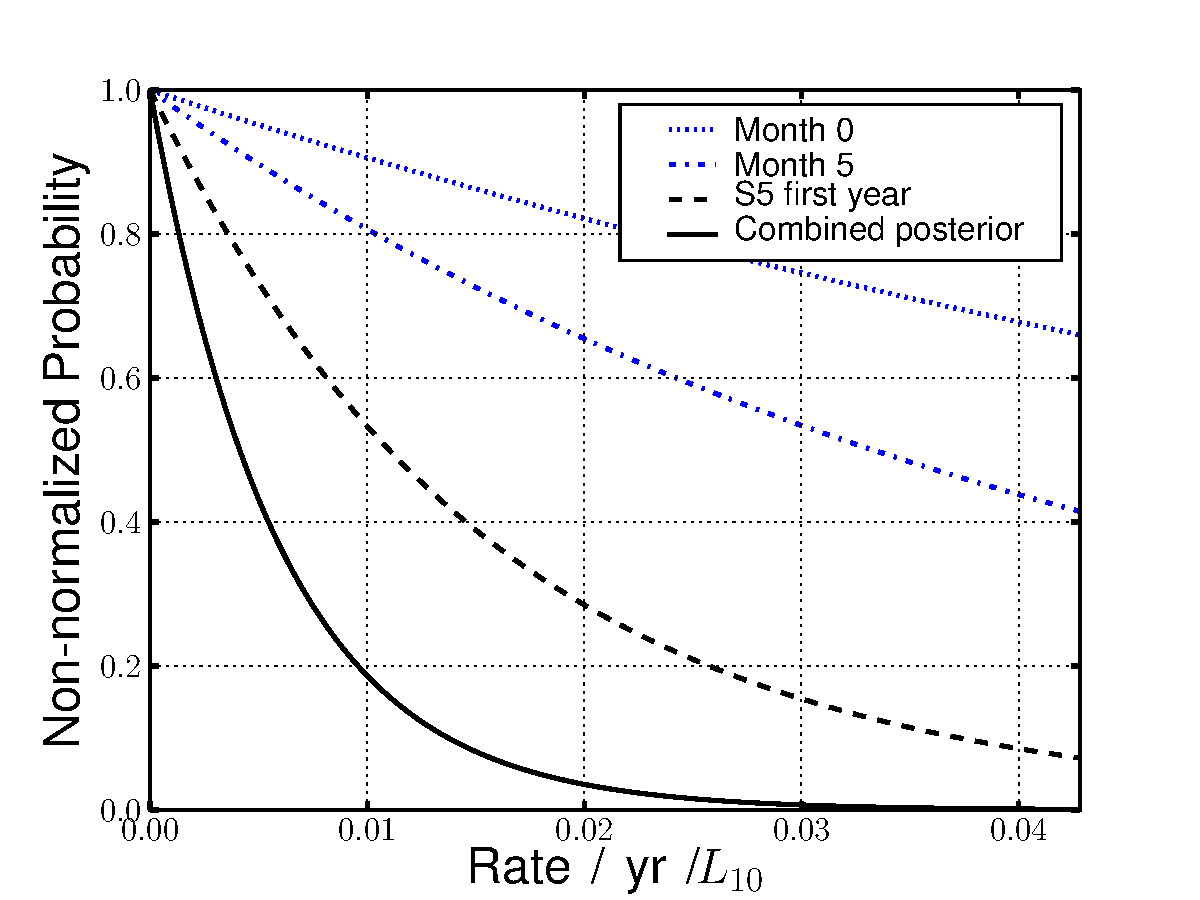
\includegraphics[width=6in]{figures/S5_lowmass_18_month_combined_bns_nonspin-posterior-comparison}
\caption{The posterior distribution for the rate of \ac{BNS} coalescences. The
dashed black curve shows the rate computed in Ref.~\cite{Collaboration:2009tt}.
The solid black curve shows the result of this search using the previous
analysis as a prior. The figure also shows the rate distributions for two of
the  individual months computed using a uniform prior. The improvement from
month 0 to month 5 is due to increasing detector sensitivity during this
search.  }  
   \label{fig:ul}
\end{figure}

The rate of instrumental noise artifacts is measured by ime-shifting data from 
the Livingston and Hanford observatories (H1 and H2 data are kept fixed with 
respect to each other). The data are offset by more than the light-travel time 
between observatories, thus triggers which survive the pipeline are due to 
noise alone. We performed 100 such time-shifts to obtain a good estimate of 
the noise background in our search. \ac{CBC} signals of higher-mass contain 
fewer gravitational-wave cycles in the sensitive band of our detectors: 
our signal-based vetoes are not as powerful. High-mass templates are therefore 
more sensitive to nonstationary noise transients and hence our \ac{FAR} for 
these system is larger. In order to account for this mass-dependent behavior 
we compute the background for three different mass regions and compare 
foreground and background within each of these ranges. Specifically, in each
region we count the number of background triggers with effective
\ac{SNR} greater than or equal to a given foreground trigger; dividing
this number by the amount of background time analyzed gives us the
\ac{FAR} for that trigger. This allows us to define a single detection
statistic for every trigger in each of the mass categories.  The
\ac{FAR} can then be directly compared to obtain a ranking of the
significance of the triggers, regardless of their
mass~\cite{Collaboration:2009tt}. 

%%%%%%%%%%%%%%%%%%%%%%%%%%%%%%%%%%%%%%%
\section{Search results}
\label{sec:results}

The seven months of data were analyzed separately using the procedure
described above. No gravitational-wave candidates were observed with a
\ac{FAR} significantly above those expected from the noise background.  The
loudest trigger in this search was a triple coincident trigger with a FAR of
$6$ per year. This is consistent with the expected background, since we
searched $0.21$~yr of data. The second and third loudest triggers had FAR
values of $10$ and $11$ per year respectively. Although we did not have any
detection candidates, we exercised our follow-up procedures by
examining any triggers with a \ac{FAR} of less than $50$ per year. 
This exercise prepares us for future detections and often identifies areas
where our search pipeline can be improved to exclude noise transients.

In the absence of detection candidates, we use our observations to set an
upper limit on the CBC rate. We follow the procedure described
in~\cite{Fairhurst:2007qj,loudestGWDAW03,Biswas:2007ni} 
and use the results reported in
Ref.~\cite{Collaboration:2009tt} as prior information on the rates.
We present five different classes of upper limits.  The
first three limits are placed on binaries of neutron stars and/or black
holes assuming canonical mass distributions for \ac{BNS} $[m_1 = m_2 =
(1.35\pm 0.04)~\Msun]$, \ac{BBH} $[m_1 = m_2 = (5\pm 1)~\Msun]$, and
\ac{NSBH} $[m_1 = (5\pm 1)~\Msun,~m_2 = (1.35\pm 0.04)~\Msun]$ systems.
We also present upper limits as a function of the total mass of the
binary and, for \ac{NSBH} binaries, as a function of the black hole
mass. We combine the results from each of the seven
months, along with the prior results from the first year analysis, in a
Bayesian manner, using the same procedure as described
in~\cite{Collaboration:2009tt}.

We first calculate upper limits on \ac{BNS}, \ac{BBH} and \ac{NSBH}
systems assuming the objects have no spin, and summarize the results
Tables \ref{tab:bns} and \ref{tab:ul}.
The rate of binary coalescences in a galaxy is expected to
be proportional to the blue light luminosity of the
galaxy~\cite{LIGOS3S4Galaxies}.  Therefore, we place limits on the rate
per $\mathrm{L}_{10}$ per year, where $\mathrm{L}_{10}$ is $10^{10}$
times the blue solar luminosity (the Milky Way contains $\sim 1.7
\mathrm{L}_{10}$~\cite{Kalogera:2000dz}).  To calculate the search
sensitivity, the analysis was repeated numerous times adding simulated
signals with a range of masses, distance and other astrophysical
parameters to the data. Table \ref{tab:ul} shows the sensitivity of 
the LIGO detectors to coalescing binaries quoted in terms 
of the horizon distance i.e., the distance at which an optimally oriented 
and located binary would produce an \ac{SNR} of 8.  
%
There are a number of uncertainties which affect the upper limit
calculation, including Monte Carlo statistics, detector calibration,
distances and luminosities of galaxies listed in the galaxy
catalog~\cite{LIGOS3S4Galaxies} and differences between the \ac{pN}
templates used to evaluate efficiency of the search and the actual
waveforms.  The effect of these errors on the cumulative luminosity are
summarized for the \ac{BNS} search in Table~\ref{tab:bns}.  We
marginalize over all of the uncertainties~\cite{Fairhurst:2007qj}
to obtain a posterior distribution on the rate of
binary coalescences.  

In Fig.~\ref{fig:ul}, we show the derived distribution of the rate of
\ac{BNS} coalescences. The distribution is peaked at zero rate
because there are no detection candidates.  We include the distribution for
all searches previous to this one (which is our prior).  In addition, we
present the result that would be obtained from each month, were it
analyzed independently of the others and of the previous searches.  This
provides an illustration of the amount that each month contributes to
the final upper limit result and demonstrates the improvement in
sensitivity of the detectors during the search.  The upper limit is
finally obtained by integrating the distribution from zero to
$\mathcal{R}_{90\%}$ so that $90\%$ of the probability is contained in the
interval.  The results obtained in this way are
%
%\begin{eqnarray}
$\mathcal{R}_{90\%,{\rm BNS}} = \BNSul\,
\textrm{yr}^{-1}\mathrm{L_{10}}^{-1} \, ,
\mathcal{R}_{90\%,{\rm BBH}} = \BBHul\,
\textrm{yr}^{-1}\mathrm{L_{10}}^{-1} \, , \text{ and }
\mathcal{R}_{90\%,{\rm NSBH}} =  \NSBHul\,
\textrm{yr}^{-1}\mathrm{L_{10}}^{-1} \, .$
%\end{eqnarray}


Additionally we calculate the upper limit for \ac{BBH} systems
as a function of the total mass of the binary, assuming a uniform
distribution of the component masses.  For \ac{NSBH} systems, we
construct an upper limit as a function of the black hole mass, assuming
a fixed neutron star mass of $m_{\mathrm{NS}} = 1.35
\Msun$.  These upper limits are shown in Fig~\ref{fig:ulmass}.

%\input{ulTable1}
\begin{table}[t]
\center
\begin{tabular}{c | c | c | c}
\hline \hline
\multicolumn{1}{m{5cm}|}{\centering Coincidence time} & H1H2L1 & H1L1 & H2L1 \\
\hline
\multicolumn{1}{m{5cm}|}{\centering Observation time (yr)} & 0.21 & 0.02 & 0.01 \\
\hline
\multicolumn{1}{m{5cm}|}{\centering Cumulative luminosity $\left({L_{10}}\right)$} & $\BNStripleCumLum$ & $\BNSHoneLoneCumLum$ & $\BNSHtwoLoneCumLum$ \\
\hline
\multicolumn{1}{m{5cm}|}{\centering Calibration error} & $\BNStripleCalErr$ & $\BNSHoneLoneCalErr$ & $\BNSHtwoLoneCalErr$ \\
\hline
\multicolumn{1}{m{5cm}|}{\centering Monte Carlo error} & $\BNStripleMonErr$ & $\BNSHoneLoneMonErr$ & $\BNSHtwoLoneMonErr$ \\
\hline
\multicolumn{1}{m{5cm}|}{\centering Waveform error} & $\BNStripleWavErr$ & $\BNSHoneLoneWavErr$ & $\BNSHtwoLoneWavErr$ \\
\hline
\multicolumn{1}{m{5cm}|}{\centering Galaxy distance error} & $\BNStripleGDErr$ & $\BNSHoneLoneGDErr$ & $\BNSHtwoLoneGDErr$ \\
\hline
\multicolumn{1}{m{5cm}|}{\centering Galaxy magnitude error} & $\BNStripleGMErr$ & $\BNSHoneLoneGMErr$ & $\BNSHtwoLoneGMErr$ \\
\hline
\hline
\end{tabular}
\caption{Detailed results from the \ac{BNS} search.  The observation
time is the time used in the upper limit analysis.  The cumulative
luminosity is the luminosity to which the search is sensitive above the
loudest event for each coincidence time.  The errors in this table are
listed as one-sigma logarithmic error bars (expressed as percentages) in
luminosity associated with each source error.}
\label{tab:bns}
\end{table}


%\input{ulTable2}
\begin{table}[t]
\center
\begin{tabular}{c | c | c | c}
\hline \hline
\multicolumn{1}{m{3cm}|}{\centering Component masses $\left(M_{\odot}\right)$} & 1.35/1.35 & 5.0/5.0 & 5.0/1.35 \\
\hline
\multicolumn{1}{m{3cm}|}{\centering $D_{\rm horizon}$ $\left({\rm Mpc}\right)$} & $\sim 30$ & $\sim 100$ & $\sim 60$ \\
\hline
\multicolumn{1}{m{3cm}|}{\centering Cumulative lminosity $\left({L_{10}}\right)$} & 490 & 11000 & 2100 \\
\hline
\multicolumn{1}{m{3cm}|}{\centering Nonspinning upper limit $\left({{\rm yr}^{-1} L_{10}^{-1}}\right)$} & \BNSul & \BBHul & \NSBHul \\
\hline
\multicolumn{1}{m{3cm}|}{\centering Spinning upper limit $\left({{\rm yr}^{-1} L_{10}^{-1}}\right)$} & ... & \SBBHul & \SNSBHul \\
\hline
\hline
\end{tabular}
\caption{Overview of results from \ac{BNS}, \ac{BBH} and \ac{NSBH}
searches.  $D_{\rm horizon}$ is the horizon distance 
averaged over the time of the search.  The cumulative luminosity is the
luminosity to which the search is sensitive above the loudest event for
times when all three \ac{LIGO} detectors were operational.  The first
set of upper limits are those obtained for binaries with nonspinning
components.  The second set of upper limits are produced using black
holes with a spin uniformly distributed between zero and the maximal
value of $G m^{2}/c$.}
\label{tab:ul}
\end{table}


\begin{figure}[ht] 
\center
\subfigure{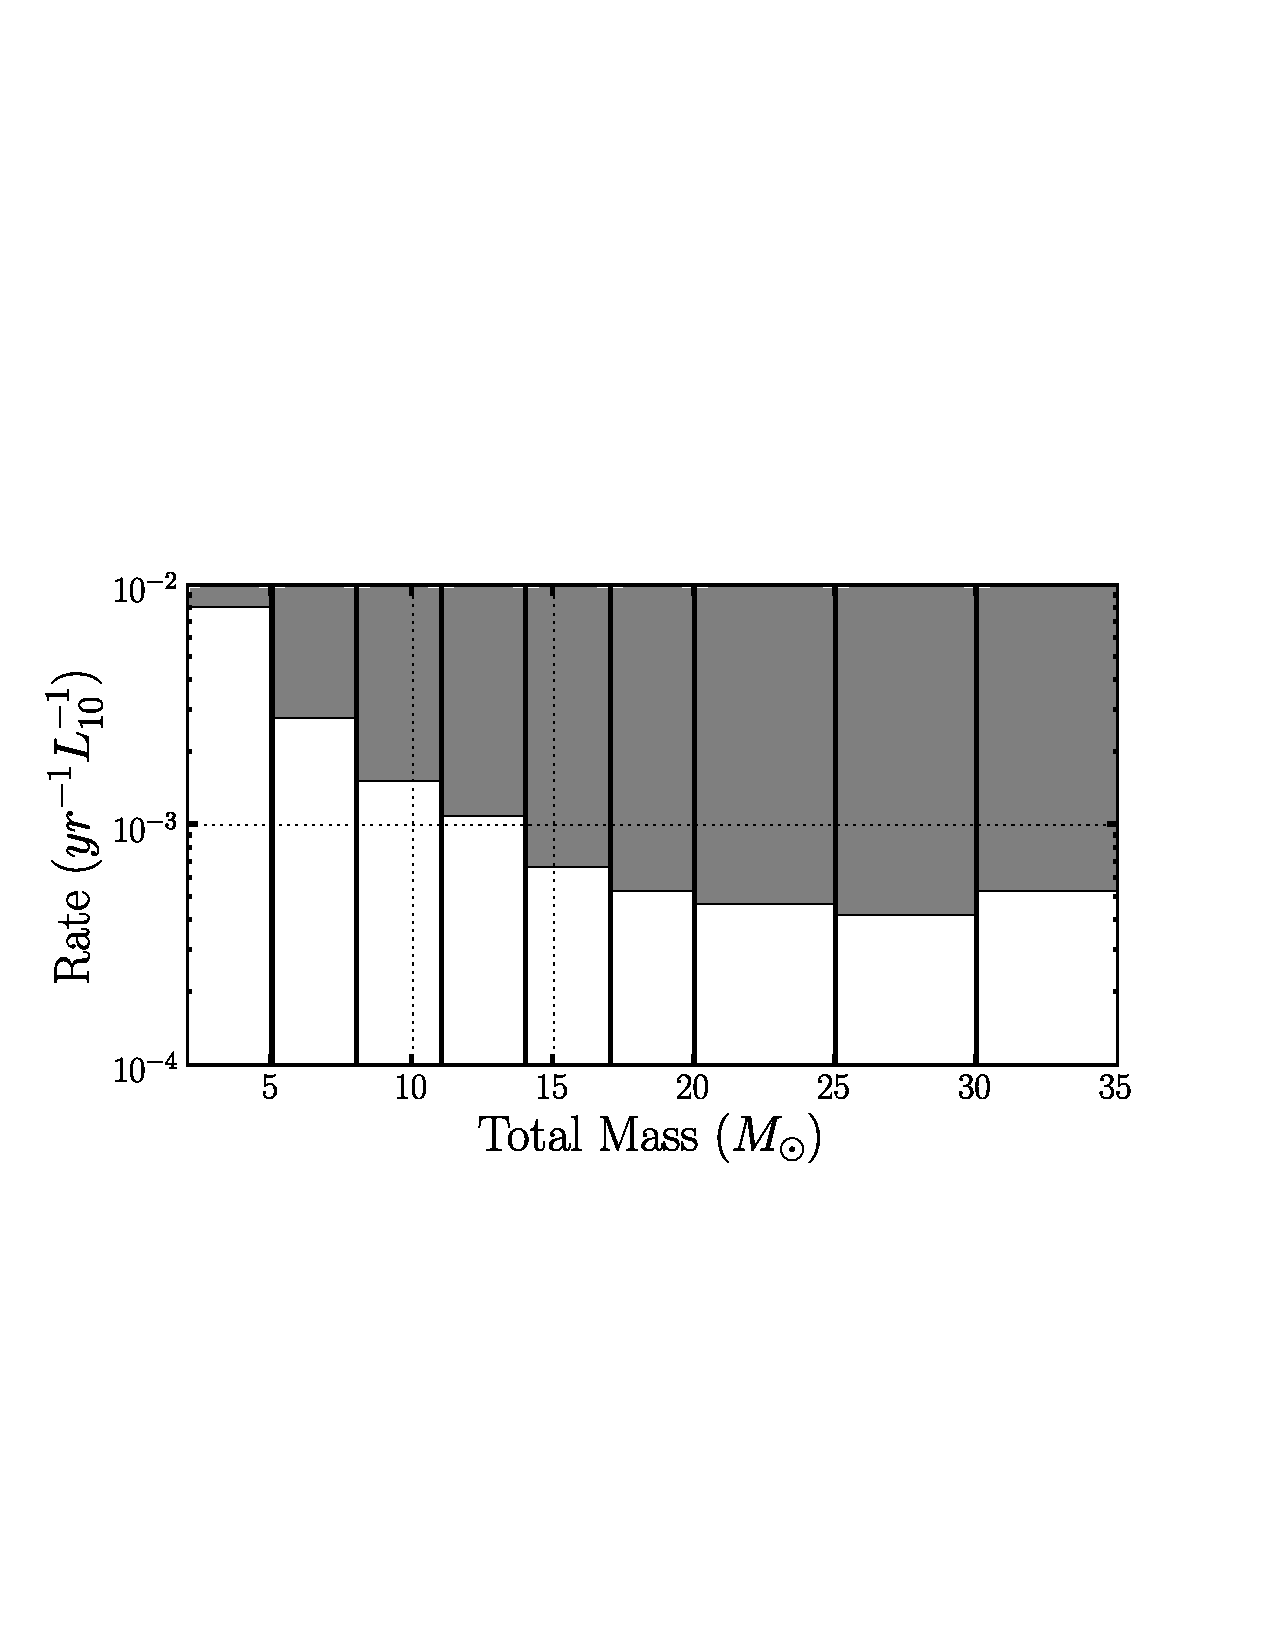
\includegraphics[width=6in]{figures/S5_lowmass_18_month_combined_mtotal_nonspin-combined-rate-v-mass}\vspace*{0.15cm}}
\subfigure{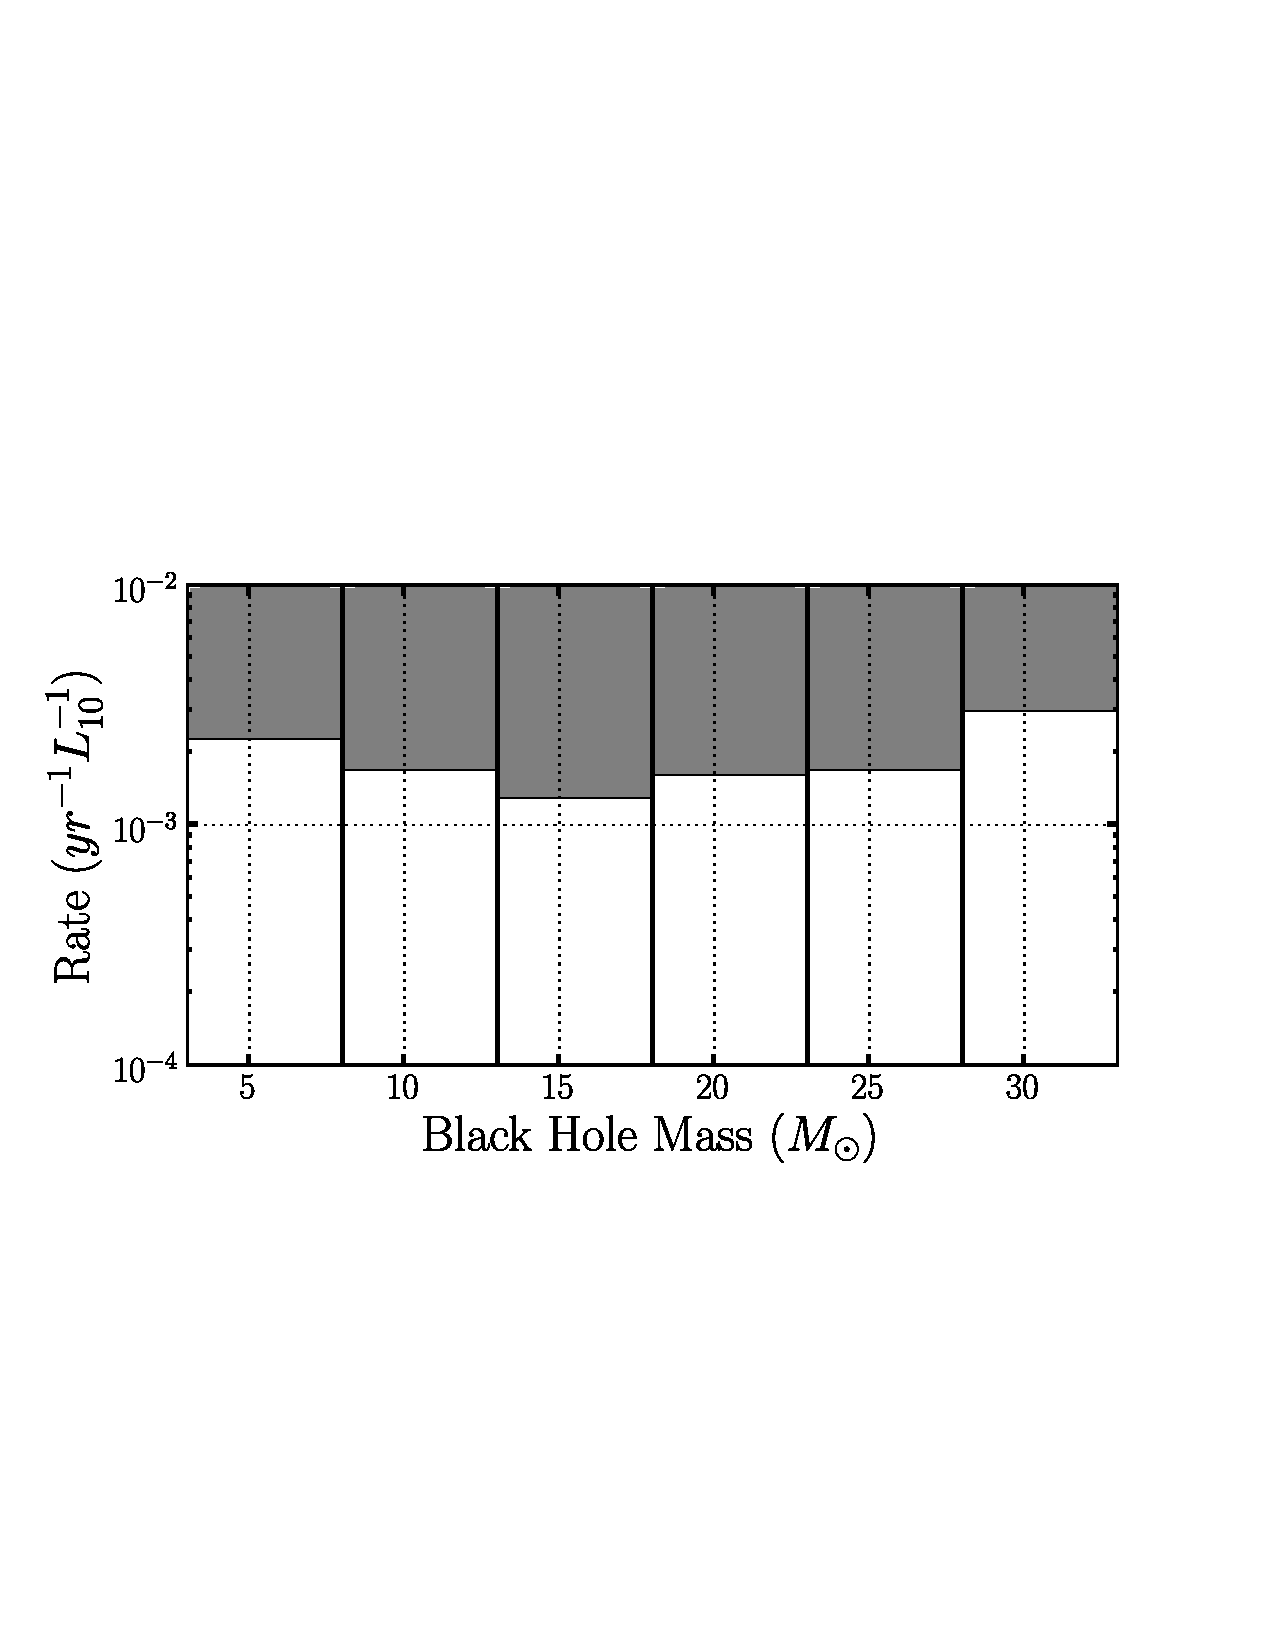
\includegraphics[width=6in]{figures/S5_lowmass_18_month_combined_mcomp_nonspin-combined-rate-v-mass}}
  \caption{The marginalized 90\% rate upper limits as a function of mass.  The
upper plot shows limits for \ac{BBH} systems as a function of the
total mass of the system.  The lower plot shows limits for \ac{NSBH}
systems as a function of the black hole mass, assuming a fixed
neutron star mass of $1.35 M_{\odot}$. Here the upper limits are 
calculated using only H1H2L1 data since the relatively small amount
of H1L1 and H2L1 data makes it difficult to 
evaluate the cumulative luminosity in the individual mass bins.} 
  \label{fig:ulmass}
\end{figure}
Finally, we present upper limits on coalescence rates where the spin of
the components of the binary is taken into account.  Astrophysical
observations of neutron stars indicate that their spins will not be
large enough to have a significant effect on the \ac{BNS} waveform
observed in the \ac{LIGO} band~\cite{ATNF:psrcat,Apostolatos:1994}.
Theoretical considerations limit the magnitude of the spin, $S$, of a
black hole to lie within the range $0 \le S \le G m^{2}/c$.  However,
the astrophysical distribution of black hole spins, and spin
orientations, is not well constrained.  Therefore, we provide a sample
upper limit for spinning systems using a spin magnitude and orientation
distributed uniformly within the allowed values.  This gives upper
limits on the rate of \ac{BBH} and \ac{NSBH} systems of
%
%\begin{eqnarray}
$\mathcal{R}_{90\%,{\rm BBH}} = \SBBHul\,
\textrm{ yr}^{-1}\mathrm{L_{10}}^{-1} \text{ and }
\mathcal{R}_{90\%,{\rm NSBH}} =  \SNSBHul\,
\textrm{ yr}^{-1}\mathrm{L_{10}}^{-1} \, .$
%\end{eqnarray}
%
These rates are about $20\%$ larger than the nonspinning rates.

\paragraph{Discussion}

We have searched for gravitational waves from CBCs with total mass
between $2$ and $35\, M_\odot$ in \ac{LIGO} observations between November
14, 2006 and May 18, 2007.  No detection candidates with significance
above that expected due to the background were found in the search. By
combining this search with our previous results, we set a new upper
limit on the CBC rate in the local universe which is approximately a
factor of $3$ lower than that reported in
Ref.~\cite{Collaboration:2009tt}.  This improvement is significant, even
though we searched only two thirds as much data as in
Ref.~\cite{Collaboration:2009tt}.  It is due, in part, to improvements
in detector sensitivity during S5 which increased the horizon distance.
Moreover, the shorter analysis time and improved stationarity of
the data, led to many of the months having a less significant loudest
event than in the previous search.  Both of these effects increased the
luminosity to which the search was sensitive, thereby improving the
upper limit.

Astrophysical estimates for \ac{CBC} rates depend on a number of
assumptions and unknown model parameters, and are still uncertain at
present.  In the simplest models, the coalescence
rates should be proportional to the stellar birth rate in nearby spiral
galaxies, which can be estimated from their blue luminosity
\cite{LIGOS3S4Galaxies}.  The optimistic, upper end of the plausible
rate range for \ac{BNS} is $5 \times 10^{-4} \textrm{ yr}^{-1}
\mathrm{L}_{10}^{-1}$~\cite{Kalogera:2004tn, Kalogera:2004nt} and $6 \times
10^{-5} \textrm{ yr}^{-1} \mathrm{L}_{10}^{-1}$ for \ac{BBH} and \ac{NSBH}
\cite{Oshaughnessy:2008, OShaughnessy:2005}.  
The upper limits reported here are $\sim 1$--$2$ orders of
magnitude above the optimistic expected rates.  With the next run starting in mid 2009, the Enhanced \ac{LIGO} and Virgo
detectors will begin operations with a factor of $\sim 2$ increase in horizon
distance. The total luminosity searched will increase by a factor of $\sim
10$, thereby bringing us close to the optimistic rates.
The most confident \ac{BNS} rate predictions are based on extrapolations
from observed binary pulsars in our Galaxy; these yield realistic
\ac{BNS} rates of $5 \times 10^{-5} \textrm{ yr}^{-1} 
\mathrm{L}_{10}^{-1}$~\cite{Kalogera:2004tn, Kalogera:2004nt}.  Rate
estimates for \ac{BBH} and \ac{NSBH} are less well constrained, but
realistic estimates are $2 \times 10^{-6} \textrm{ yr}^{-1} 
\mathrm{L}_{10}^{-1}$ for \ac{NSBH} \cite{Oshaughnessy:2008} and $4
\times 10^{-7} \textrm{ yr}^{-1} \mathrm{L}_{10}^{-1}$ for \ac{BBH}
\cite{OShaughnessy:2005}.  Thus, the expected rates are $\sim 2$--$3$
orders of magnitude lower than the limits presented in this paper. The
Advanced LIGO and Virgo detectors, currently under construction, will
increase our horizon distance by an order of magnitude or more, allowing us to
measure the rate of CBCs in the Universe.

\section{Acknowledgements}
The authors gratefully acknowledge the support of the United States
National Science Foundation for the construction and operation of the
LIGO Laboratory and the Science and Technology Facilities Council of the
United Kingdom, the Max-Planck-Society, and the State of
Niedersachsen/Germany for support of the construction and operation of
the GEO600 detector. The authors also gratefully acknowledge the support
of the research by these agencies and by the Australian Research Council,
the Council of Scientific and Industrial Research of India, the Istituto
Nazionale di Fisica Nucleare of Italy, the Spanish Ministerio de
Educaci\'on y Ciencia, the Conselleria d'Economia, Hisenda i Innovaci\'o of
the Govern de les Illes Balears, the Royal Society, the Scottish Funding 
Council, the Scottish Universities Physics Alliance, The National Aeronautics 
and Space Administration, the Carnegie Trust, the Leverhulme Trust, the David
and Lucile Packard Foundation, the Research Corporation, and the Alfred
P. Sloan Foundation.




\Chapter{S6 Tuning and Results}
\label{ch:s6_results}
% s6results.tex

% loudest FARs
\def\firstFAR{\ensuremath{\mathrm{2.2~yr^{-1}}}}
\def\secondFAR{\ensuremath{\mathrm{5.6~yr^{-1}}}}
\def\thirdFAR{\ensuremath{\mathrm{9.4~yr^{-1}}}}
\def\expectedLoudestFAR{\ensuremath{\mathrm{\sim2~yr^{-1}}}}
\def\dogDate{16 September 2010}
\def\injectedDogTime{06:42:23 UTC}
\def\injectedDogGPSTime{968654558.0}

The sixth \ac{LIGO} Science (S6) run began on 7 July 2009 and ended on 20
October 2010. This observing run overlapped with two separate Virgo Science
runs: Virgo's second science run (VSR2), which ran from 7 July 2009 to 11
January 2010, and Virgo's third science run (VSR3), which ran from 11 August
2010 to 20 October 2010. A number of improvements were made in both detector
hardware and \ac{CBC} analysis software between \ac{S5} and \ac{S6}. The
software improvements have already been described in prior chapters: New
\ac{SNR} was developed to replace effective \ac{SNR}, and Pipedown was
implemented.

In this chapter we describe the \ac{S6} and VSR2/3 analysis. Section
\ref{sec:hardware_improvements} describes the hardware improvements made to the
detectors between \ac{S5} and \ac{S6}. In section \ref{sec:s6_epochs} we
describe each of the four epochs the analysis was broken into. Section
\ref{sec:dq_issues} details some of the major data quality (DQ) issues that
arised during S6/VSR2/3 and how they were dealt with, along with tuning
decisions made. In this section we give an example of a veto developed from the
loudest-slide studies that were implemented in the second half of \ac{S6}.
Finally, in section \ref{sec:s6_results_and_big_dog} we give the results of the
search. No gravitational waves from \acp{CBC} were detected. We describe a
\emph{blind injection} that was made, and found, during S6/VSR3.  Upper limits
on the rate of \acp{CBC} will be presented in a forthcoming \ac{LSC} and Virgo
publication \cite{Collaboration:S6CBClowmasss}.

\section{Hardware Improvements}
\label{sec:hardware_improvements}

The two $4\,$km \ac{LIGO} interferometers, H1 and L1, were used for \ac{S6}.
The $2\,$km Hanford detector, H2 was not operational during this run. Several
hardware changes were made to the \ac{LIGO} detectors so that prototypes of
Advanced LIGO technology could be installed and tested. This included the
installation of a more powerful, $35\,\mathrm{W}$ laser, and the implementation
of a DC readout system that included a new Output Mode Cleaner on an Advanced
LIGO seismic isolation table~\cite{Adhikari:2006}. In addition, the hydraulic
seismic isolation system was improved by fine-tuning its feed-forward path.
Known as ``HEPI feed-forward," this improvement was implemented in January of
2010; it is described in more detail in section \ref{sec:s6b}, below.

Several hardware enhancements were also made to the Virgo detector in the
period between \ac{VSR1} and \ac{VSR2}. A more powerful laser was installed,
along with a thermal compensation system and scattered light was better
mitigated. During early 2010, monolithic suspension was installed, which
involved replacing Virgo's test masses with new mirrors hung from fused-silica
fibers. Following this upgrade Virgo began \ac{VSR3}. 

The average sensitivity of the detectors to binary coalescence signals in each
epoch is shown in Figures \ref{fig:s6a_insprange} -- \ref{fig:s6d_insprange}.
These figures show the distance at which an optimally oriented and located
binary would produce a \ac{SNR} of $8$ in a given detector. The figures show
how the detectors were improved over the course of the run, and they eventually
surpassed the best \ac{S5} ranges. 

\section{S6 Epochs}
\label{sec:s6_epochs}

\ac{S6} and VSR2/3 were broken into four epochs: \emph{S6A}, which ran from 7
July 2009 to 1 September 2009; \emph{S6B}, 24 September 2009 to 11 January
2010; \emph{S6C}, 6 February 2010 to 25 June 2010; \emph{S6D}, 26 June 2010 to
20 October 2010. Table \ref{tab:s6-livetimes} lists the analyzed time (live
time) and duty cycle in each epoch after CAT3 vetoes\footnote{See section
\ref{sec:PipelineRequirements} for definition of vetoes and veto categories.}
have been applied. Across all of S6 we analyzed $0.48$ years of data, giving a
duty cycle of $0.41$.

Figure \ref{fig:s6_insprange_v_time} shows a plot of the \ac{BNS} inspiral
range (with each component mass $= 1.4\,\Msun$) across all of \ac{S6} and the
span of each epoch. The start and end times of the epochs were based on a
combination of instrumental and analysis factors. S6A ended at a pre-planned
commissioning break to try to improve the detectors after learning lessons from
the first two months of running. S6B ran from the end of the commissioning
break until the end of \ac{VSR2}. At this point, Virgo was taken off line for
eight months in order to install the monolithic suspension. S6C therefore
consisted only of coincident time between Hanford and Livingston. Another
commissioning break was taken at the end of S6B, hence the gap between the end
of S6B and the start of S6C. S6D was to begin when Virgo came back online in
August of 2010. During S6C we noticed that non-Gaussian noise transients
(\emph{glitches}) often created triggers with \acp{SNR} above threshold when
match filtered with templates that had total masses $> 25\,\Msun$. Thus we
decided to lower the mass-range of our template bank\footnote{Recall from
section \ref{sec:multiple_templates} that a template bank is the collection of
waveforms we use to match filter the data.} from $2 \leq \mtotal/\Msun \leq 35$
to $2 \leq \mtotal/\Msun \leq 25$. We wanted to do this as soon as possible,
and so the somewhat arbitrary date of 26 June 2010 was chosen as the break
between S6C and S6D. Aside from Virgo coming back online, there were no major
instrumental adjustments between S6C and D. There were, however, new vetoes
implemented for S6D based on \ac{CBC} results in S6C. These new vetoes, as well
as more details about the decision to decrease the range of the template bank,
are discussed in section \ref{sec:dq_issues}. In the next few sections we give
more details about each of the epochs.

\begin{table}[hbtp]
\center
\begin{tabular}{| c | c | c | c | c | c | c |}
\hline
\multirow{2}{*}{Epoch}   &  \multicolumn{4}{|c|}{Live Time by Instrument Time (days)}  &   \multirow{2}{*}{\parbox{2.3cm}{Total Live Time (days)}}  &    \multirow{2}{*}{Duty Cycle} \\
\cline{2-5}
    &  H1L1  &   H1V1   &   L1V1   &     H1L1V1 &   &   \\
\hline \hline
S6A     &   1.2 &   10.9    &   10.0    &   7.1  &   29.2    &   0.53 \\
\hline
S6B     &   7.1 &   20.6    &   9.4     &  10.6  &   47.7    &   0.44 \\
\hline
S6C     &   39.3    &   --  &   --      &   --   &   39.3    &   0.28 \\
\hline
S6D     &   22.6    &   7.7 &   8.3     &   19.7 &   58.3    &   0.50 \\
\hline \hline
Total   &   70.2    &   39.1 &  27.7    &   37.4 &   \textbf{174.5}   &   \textbf{0.41} \\
\hline
\end{tabular}
\caption{The analyzed time (\emph{live time}) in each epoch, and the total for S6/VSR2/3. All times are calculated after CAT3 vetoes have been applied.}
\label{tab:s6-livetimes}
\end{table}

\begin{landscape}
\begin{figure}[p]
\begin{center}
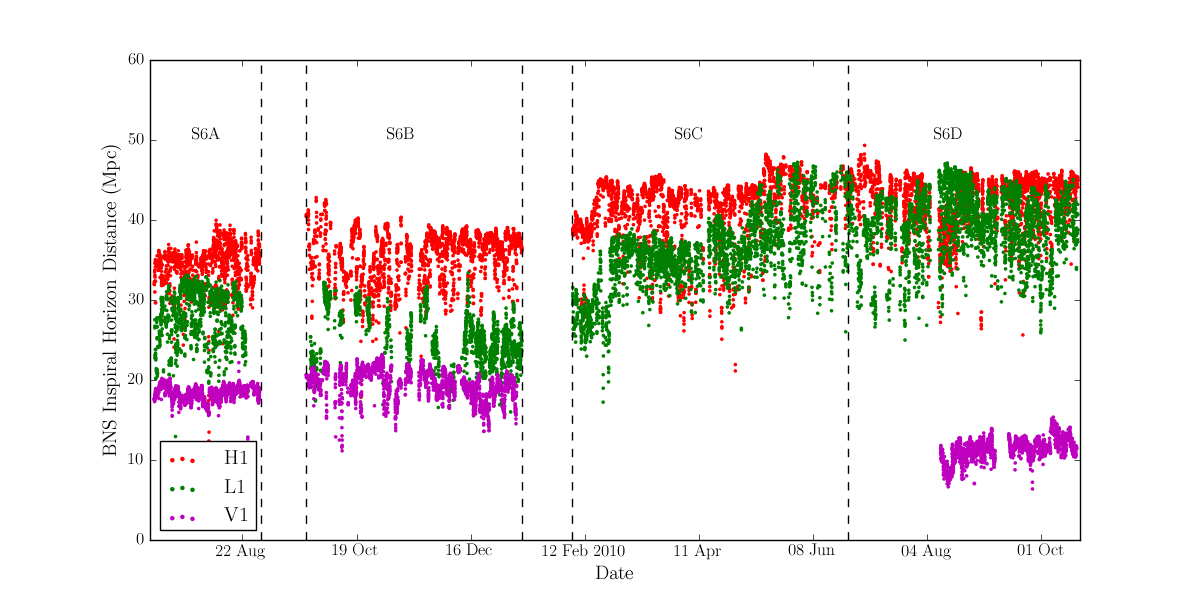
\includegraphics[width=9in]{figures/s6-hzrange_v_time.png}
\end{center}
\caption{The inspiral range for a $1.4/1.4\,\Msun$ \ac{BNS} system at \ac{SNR} $8$ in each \ac{IFO} across \ac{S6}. The range is computed by \texttt{lalapps\_tmpltbank} using equation \ref{eqn:DtoRho}. Each dot represents the range in a $2048\,$s--long analysis chunk.}
\label{fig:s6_insprange_v_time}
\end{figure}
\end{landscape}

\clearpage

\begin{figure}[p]
\begin{center}
\label{fig:s6a_insprange}
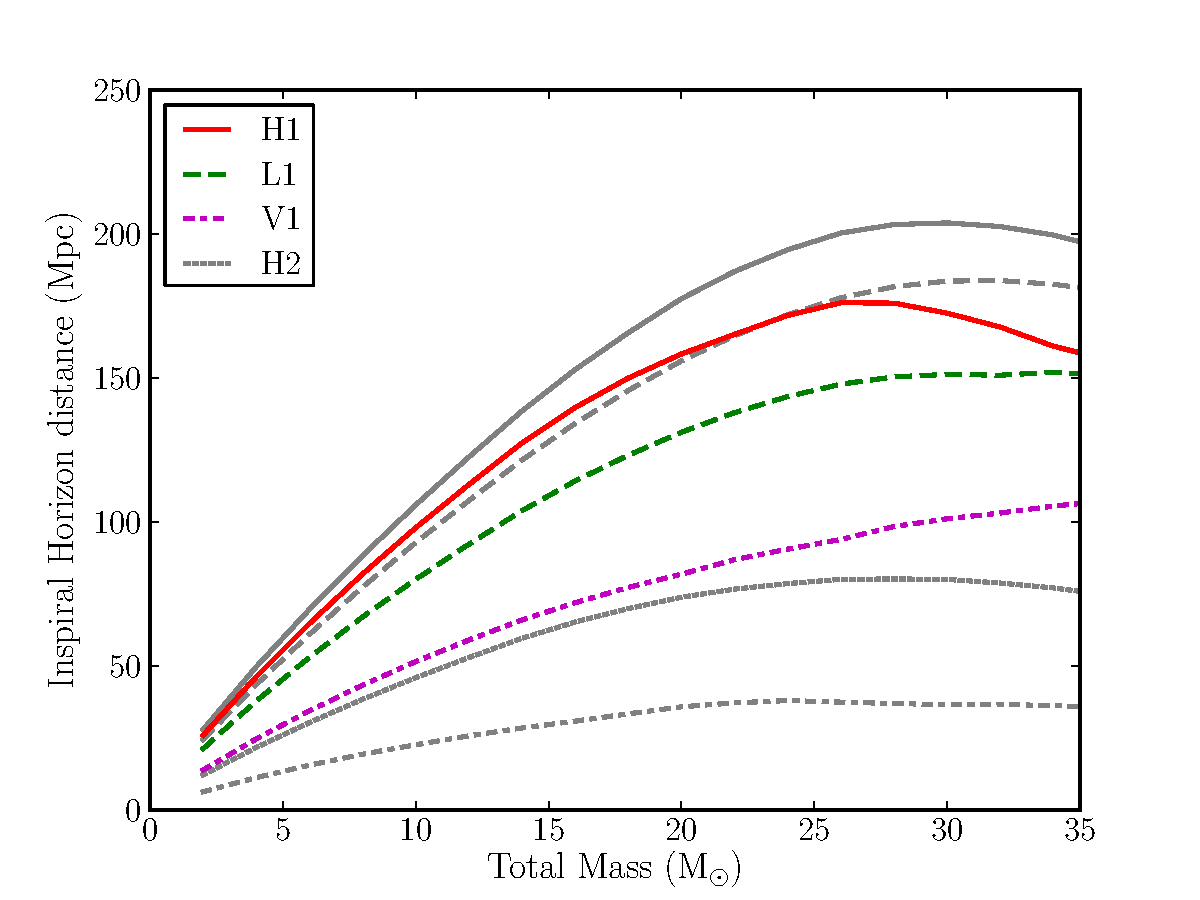
\includegraphics[width=6in]{figures/s6a_insprange.pdf}
\end{center}
\caption{Average inspiral range of S6A. Ranges were computed by \texttt{lalapps\_tmpltbank} using equation \ref{eqn:DtoRho} with $\rho=8$, then averaged over all analysis chunks in the epoch. S6 ranges are in color; best S5 ranges are in gray. Although H2 was not used in \ac{S6}, it is shown for comparison to V1.}
\end{figure}

\begin{figure}[p]
\begin{center}
\label{fig:s6b_insprange}
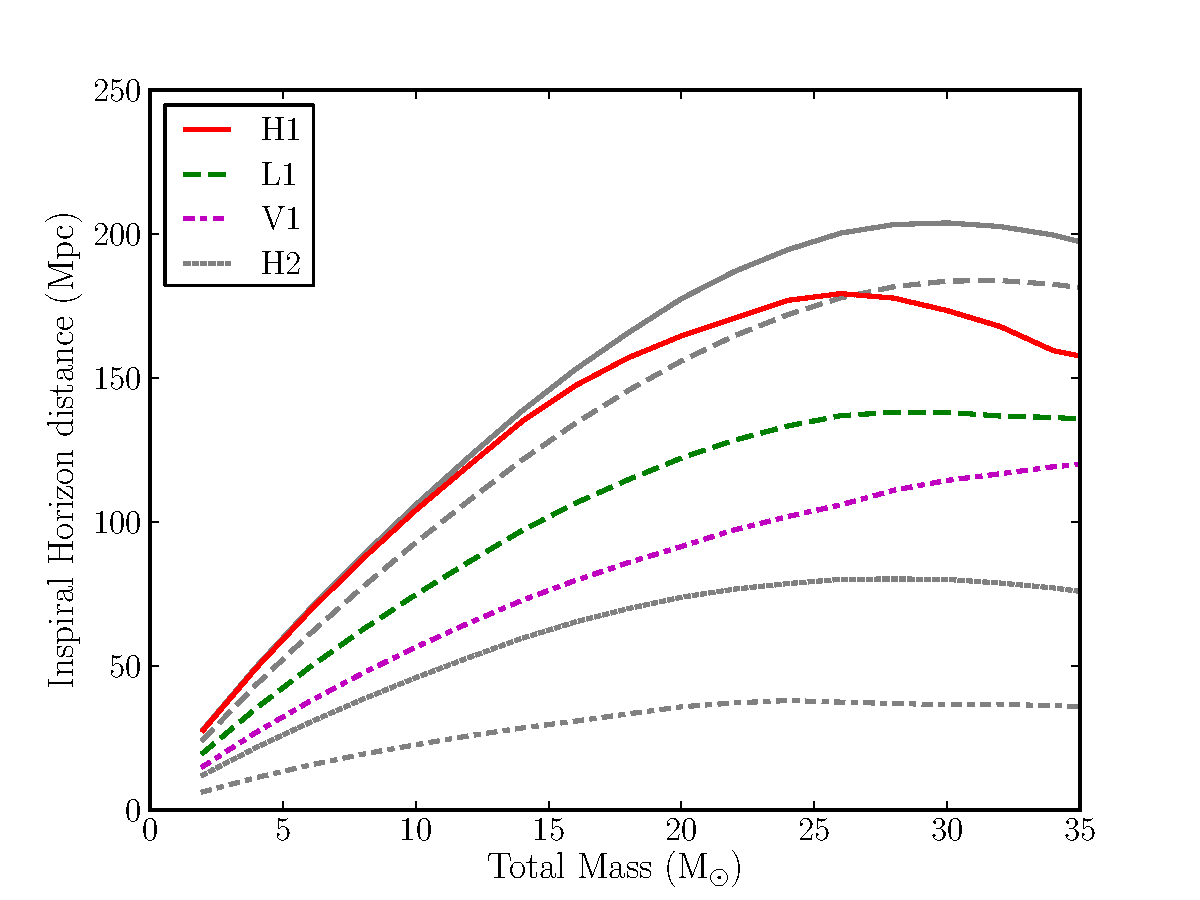
\includegraphics[width=6in]{figures/s6b_insprange.pdf}
\end{center}
\caption{Average inspiral range of S6B. Ranges were computed using the same method as in Figure \ref{fig:s6a_insprange}.}
\end{figure}

\begin{figure}[p]
\begin{center}
\label{fig:s6c_insprange}
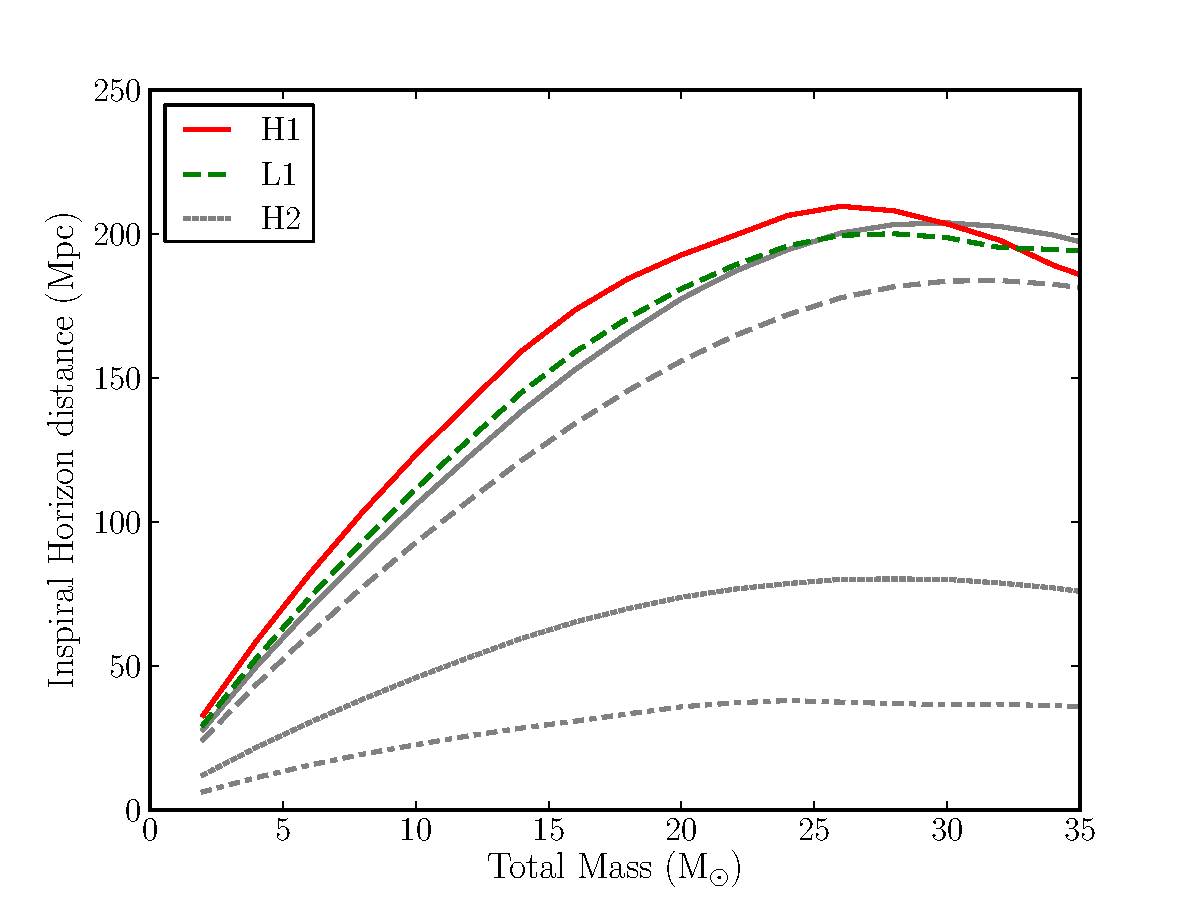
\includegraphics[width=6in]{figures/s6c_insprange.pdf}
\end{center}
\caption{Average inspiral range of S6C. V1 is not shown as it was down for commissioning during this period. Ranges were computed using the same method as in Figure \ref{fig:s6a_insprange}.}
\end{figure}

\begin{figure}[p]
\begin{center}
\label{fig:s6d_insprange}
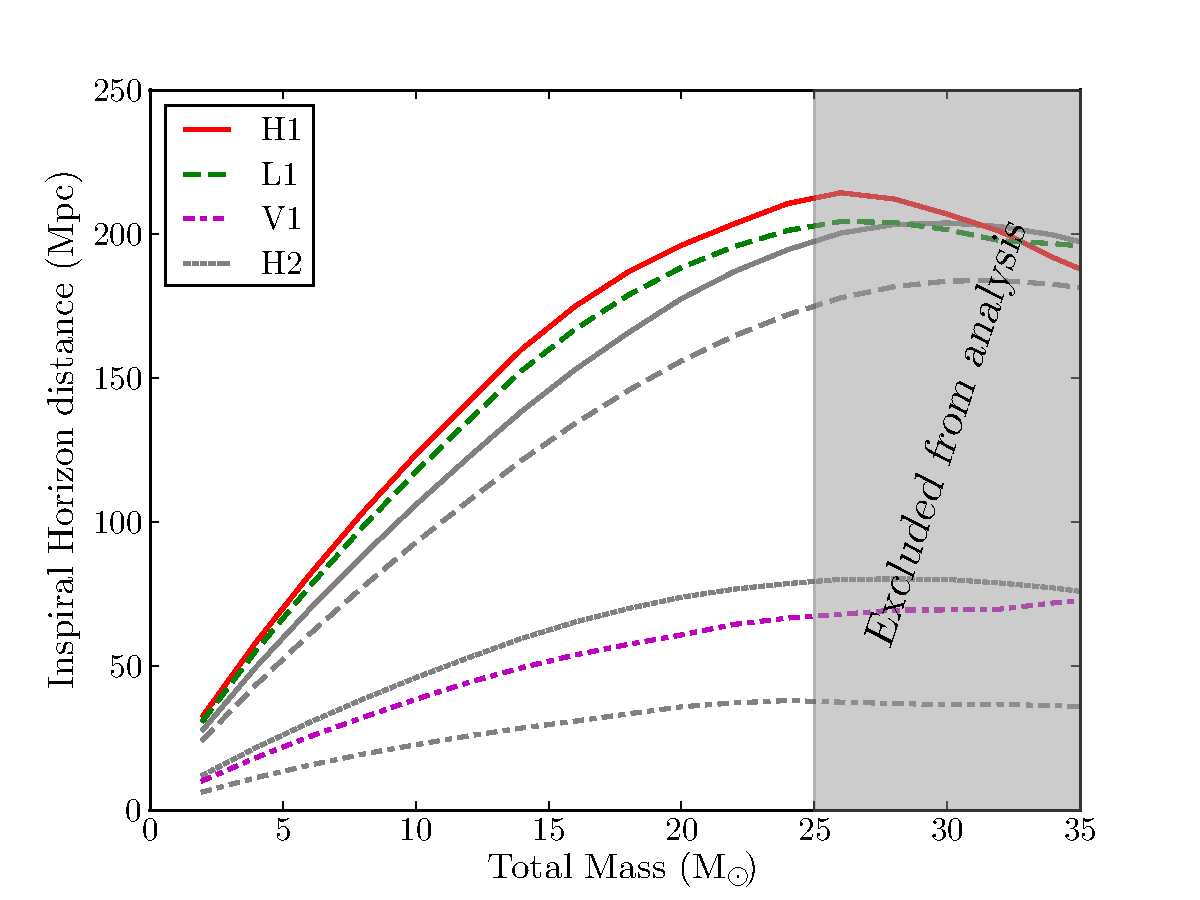
\includegraphics[width=6in]{figures/s6d_insprange_alt.pdf}
\end{center}
\caption{Average inspiral range of S6D. Shaded region indicates the mass range that was excluded in the low mass search for this period. Ranges were computed using the same method as in Figure \ref{fig:s6a_insprange}.}
\end{figure}

\subsection{S6A}
\label{sec:s6a}

At the start of the S6 Science run, the \ac{LIGO} detectors had lower
sensitivity and more glitches than in later epochs. This can be seen in Figure
\ref{fig:s6_insprange_v_time}. In fact, the S6A \ac{LIGO} ranges were somewhat
lower than they had been during their peak sensitivity in \ac{S5}. Figure
\ref{fig:s6a_insprange} shows the average inspiral range versus binary total
mass during S6A as compared to best ranges of \ac{S5}. We can see that Virgo,
however, showed much improvement over VSR1.

In the joint LIGO and Virgo search that occurred during \ac{VSR1} and the last
five months of \ac{S5} (the ``S5-LV" search), false alarm rates (FARs) were
based on a likelihood statistic that took into account the relative
sensitivites of various interferometer combinations. The sensitivies were used
to apply a weighting factor to each coincidence type so that more senstive
detector combinations were promoted, allowing false alarm rates to be computed
once across all combinations (as opposed to using equal-weighted bins to
compute combined \acp{FAR} from uncombined, as described in Chapter \ref{far})
\cite{S5LowMassLV}. This was implemented for two main reasons: first, with both
H2 and V1 active, four interferometers had to be analyzed, which led to a large
number of coincidence types and coincident-detector times to consider. Second,
Virgo's sensitivity was much lower than the \ac{LIGO} detectors in VSR1, and,
due to high amounts of low-frequency noise, its low-frequency cutoff had to be
set to $60\,$Hz. Thus its template bank was truncated to have a maximum chirp
mass of $\sim2.6\,\Msun$ \cite{S5LowMassLV}. The probability that various
coincidence types detected a \ac{GW} was therefore far from equal, and so
re-weighting of triggers' \acp{SNR} needed to be applied. As can be seen in
Figure \ref{fig:s6a_insprange}, however, the range of V1 was substantially
better in \ac{VSR2} --- better than H2 --- and we were able to lower its
low-frequency cutoff so that it could cover the same mass range as \ac{LIGO}.
Essentially, V1 in S6 had taken the place of H2 in S5. Further, since V1 was
not co-located with the other detectors, we could slide all the instruments
against each other, which allowed us to analyze all instrument times. (Recall
from the last chapter that H1 and H2 could not be slid against each other
because they were co-located, and so H1H2-coincident time could not be
analyzed.) For these reasons, and the fact that the \ac{S5}-LV likelihood
method was still being developed when S6A started, we decided to analyze
\ac{S6} in the same manner as in the \ac{S5} search described in Chapter
\ref{ch:s5_results} (the ``12-18 month search"\footnote{The name 12-18 month
comes from the fact that that search covered months 12 to 18 of S5.}), using
combined \ac{FAR} as our ranking statistic, and with all the coincidence types
being given equal weight. We also used many of the same tuning parameters as
the \ac{S5} 12-18 month search: the \ac{SNR} cut, $\chi^2$ and $r^2$ veto
thresholds, chirp-mass bins, and size of the e-thinca parameter\footnote{See
chapters \ref{ch:pipeline_principles} and \ref{ch:far} for definitions of these
parameters.} all remained the same.

There were a few minor adjustements, however. As mentioned in Chapter
\ref{ch:pipeline_principles}, we switched to using 3.5 restricted \ac{pN}
templates, although the template bank metric was still calculated using the
2\ac{pN} approximation. New \ac{SNR} was implemented as our ranking statistic
for computing uncombined \acp{FAR} after it was noticed --- in the 12-18 month
search and the S6A \ac{CBC} high-mass search\footnote{Recall from Chapter
\ref{ch:introduction} that the \ac{CBC} high-mass search covers the mass ranges
$25 \leq \mtotal/\Msun \leq 100$} --- that effective \ac{SNR} tended to
over-weight triggers with statistically low $\chi^2$ values. Pipedown replaced
older, more cumbersome, scripts to do post-\hipe~processing. As discussed in
Chapter \ref{ch:ihope_pipeline}, we decided to do coincidence clustering within
each chirp-mass bin as opposed to across all bins, as done in the 12-18 month
search. We also switched algorithms for computing combined \acp{FAR} from the
method discussed in section \ref{sec:alternate_cfar_method} of Chapter
\ref{ch:far} to using slide triggers' uncombined \acp{FAR}, discussed in
section \ref{sec:far-multiple_templates}. This change had little effect on the
analysis, as they are equivalent. In the 12-18 month search, \ihope~was run on
month-long blocks of data as opposed to the year-long block used in the \ac{S5}
first-year search. As discussed in Chapter \ref{ch:s5_results}, the duration of
\ihope~analysis periods were decreased to better reflect changing detector
behavior. We continued this trend of decreasing the analysis periods in
\ac{S6}: in S6A we decided to run \ihope~in week-long periods, with a different
analyst being in charge of each analysis period. Thus, S6A was (initially)
broken into 8 week-long runs.

Initially we also planned to use TrigScan clustering\footnote{See section
\ref{sec:first_inspiral} in Chapter \ref{ch:ihope_pipeline} for a description
of TrigScan clustering.} in \verb|lalapps_inspiral|\footnote{Recall from
Chapter \ref{ch:ihope_pipeline} that \texttt{lalapps\_inspiral} is the program
we use to perform match filtering.} to cluster triggers across templates.
However, we were surprised to find that trigger rates were much higher than in
\ac{S5}. TrigScan clustering was unable to keep the rate low-enough for many
\texttt{inspiral} jobs to finish (recall from Chapter \ref{ch:ihope_pipeline}
that a disadvantage of trigscan is that it cannot garauntee a maximum trigger
rate). Many jobs took several days to complete, or would simply run out of
memory. As a result, only two weeks out of the eight were able to finish with
TrigScan. Figure \ref{fig:avg_rate_per_tmplt} shows a comparison of the average
trigger rate-per-template between one of the weeks that finished (``S6aWk3")
and one of the months from the \ac{S5}-LV analysis (``lvMonth8") at each stage
of the pipeline. The rate was clearly higher for both H1 and L1 at all stages
in the pipeline. In particular, the rate at second inspiral (2 on the x-axis)
was not much lower than first inspiral (0 on the x-axis), implying that
$\chi^2$ was being calculated for a large number of triggers.\footnote{Refer to
Chapter \ref{ch:ihope_pipeline} for a description of each of these steps in the
\ihope~pipeline.} As this comparison had to use one of the weeks that finished,
the other weeks that did not finish most likely had an even higher rate as
compared to \ac{S5}.

To mitigate the high rates we decided to switch from TrigScan to time-window
clustering, discussed in section \ref{sec:first_inspiral}. What size window to
use was an open question and so we used the two weeks that completed to
investigate various clustering windows. We aimed to find the smallest window
that allowed the search to continue, and that resulted in the most efficient
recovery of vetoes. Three windows were considered: $10\,$ms, $30\,$ms, and
$100\,$ms. The $10\,$ms window was found to be too short: the trigger rates
were still too high for many runs to complete. This left the $30\,$ms and
$100\,$ms windows. Figure \ref{fig:roc_cluster_windows} shows a ROC
plot\footnote{Refer to section \ref{sec:plotroc} for a description of ROC
plots.} using $30\,$ms and $100\,$ms clustering. Note that in this plot we also
considered raising the low-frequency cutoff to $65\,$Hz. As can be seen, the
$30\,$ms window with the standard $40\,$Hz low-frequency cutoff provided the
best results. We therefore decided to use the $30\,$ms clustering for all of
\ac{S6}. Why TrigScan clustering did not work as well is an open question. It
may have simply been due to the high trigger rate. Another possibility is the
switch from 2\ac{pN} to 3.5\ac{pN} templates somehow affected its ability to
properly cluster \cite{Pekowsky:thesis}. We plan to re-address this before
Advanced \ac{LIGO}.

\begin{figure}[p]
\center
\subfigure[H1]{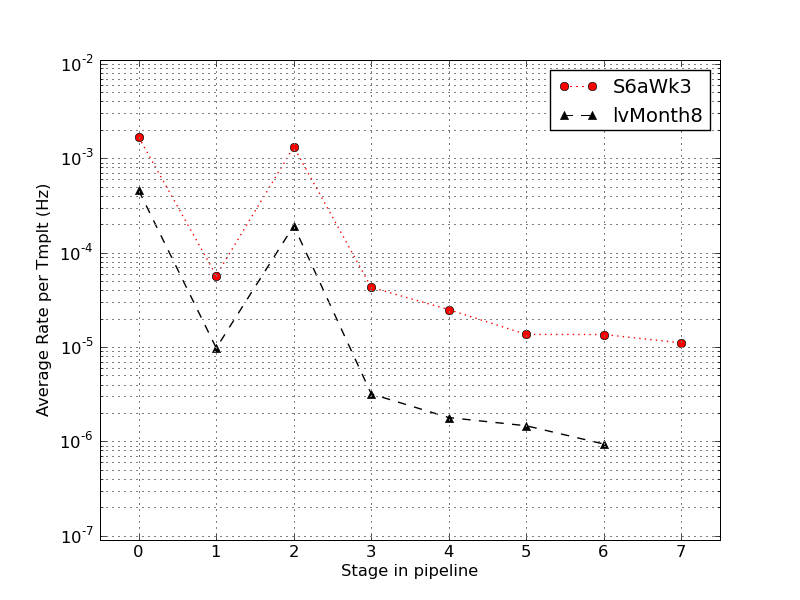
\includegraphics[width=2.8in]{figures/s6_clusterwin_investigation/H1_average_rate_per_tmplt_comparisons.png}}
\subfigure[L1]{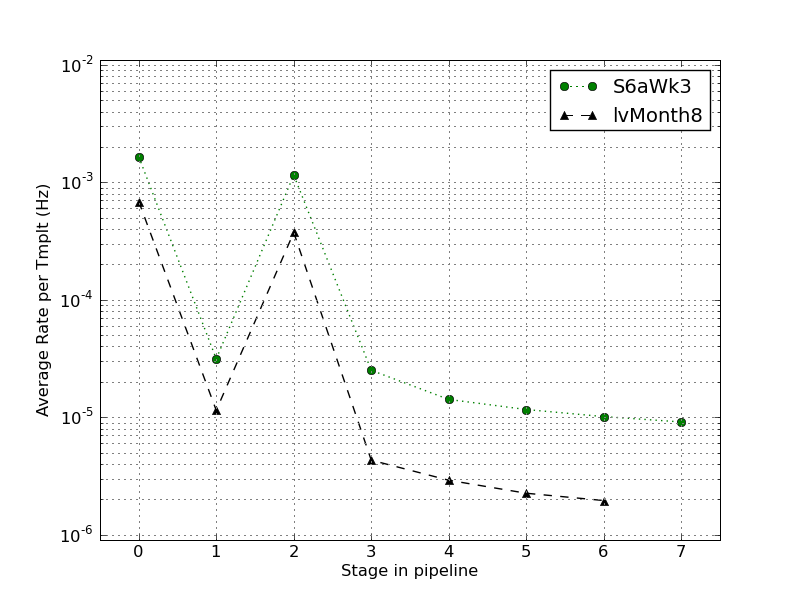
\includegraphics[width=2.8in]{figures/s6_clusterwin_investigation/L1_average_rate_per_tmplt_comparisons.png}}
\subfigure[V1]{\includegraphics[width=2.8in]{figures/s6_clusterwin_investigation/V1_average_rate_per_tmplt_comparisons.png}}
\label{fig:avg_rate_per_tmplt}
\caption{The average trigger rate per template in week 3 of S6A as compared to
one month from the S5-LV analysis. Each point represents a different stage in
the pipeline: $0 \rightarrow$ \texttt{INSPIRAL\_FIRST}, $1 \rightarrow$
\texttt{THINCA\_FIRST}, $2 \rightarrow$ \texttt{INSPIRAL\_SECOND}, and $3
\rightarrow$ \texttt{THINCA\_SECOND}. (See Chapter \ref{ch:ihope_pipeline} for
a description of each of these stages.) Stages $4$--$7$ represent the
higher-category vetoes being applied at \texttt{THINCA\_SECOND}; there is an
extra stage in S6A because hardware injections were removed by an extra
veto-category (between steps $5$ and $6$), whereas in the LV search hardware
injections were removed as a part of the CAT2 vetoes (at step $4$).}
\end{figure}

\begin{figure}[p]
\label{fig:roc_cluster_windows}
\center
\includegraphics[width=5in]{figures/s6_clusterwin_investigation/s6week3cat4_ROC.png}
\caption{ROC plot from week 3 of S6A using various clustering windows and low-frequency cutoffs.}
\end{figure}

\subsection{S6B}
\label{sec:s6b}

S6B began after the commissioning break in September of 2009. While the
sensitivity in H1 improved slightly, the sensitivity in L1 was lower than in
S6A. Further, due to inclement weather, L1 struggled to stay in Science mode
for most of the period, and so the duty cycle was much lower. As stated above,
S6B ran from September to January. Fall brings a number of storms to the Gulf
of Mexico, resulting in increased \emph{microseismic} ($0.1$--$0.35$ Hz) noise.
The effects of this noise can be seen in Figure \ref{fig:s6_insprange_v_time}:
note that L1 is off for large periods of time, and that it has lower
sensitivity when it is in Science mode.

To mitigate the seismic problem at Livingston Hydraulic External Pre-Isolation
(HEPI) feed-forward was developed during S6B. Many of the interferometer's
optics sit on tables housed in vacuum chambers. These chambers are situated on
hydraulic actuators, which are used to actively dampen seismic noise. In the
feed-forward process, the output from seismometers on the floor were fed into
the actuators to cancel out the seismic motion \cite{Lundgren:personal-comm}.
The digital filters used in the feed-forward were implemented and tuned across
S6B. This led to L1 becoming more stable, allowing for longer Science mode
periods. The effect can be seen in Figure \ref{fig:s6_insprange_v_time}: a few
days prior to 16 December L1 begins to stay in Science mode for longer periods
of time. The increased stability eventually also allowed the laser power to be
increased to $14\,$W\footnote{The laser power was set to $14\,$W at both H1 and
L1 during the evening and on weekends --- when there was little seismic noise
from human activity --- throughout S6C and D. During working hours, the laser
was typically set to $10\,$W.} which in turn led to better
range.\footnote{Recall from Chapter \ref{ch:theory}, increasing laser power
decreases shot noise.}

Due to the sensitivity of the \ac{LIGO} detectors and L1's low duty cycle, we
decided to analyze S6B in three analysis periods. The first lasted from the
start of S6B until 11 November 2009, at which point the detectors were
re-calibrated. The second and third periods ran from 11 November to 11
December, and 11 December to 11 January, respectively. We chose 11 December to
end the second period so that each period was approximately the same duration.

\subsection{S6C}
\label{sec:s6c}

After V1 went offline in January of 2010, another commissioning break was taken
to improve the sensitivity of the \ac{LIGO} detectors. Thus the S6C analysis
began approximately two weeks after the end of S6B, on 6 February. As can be
seen in Figures \ref{fig:s6_insprange_v_time} and \ref{fig:s6c_insprange}, the
commissioning throughout S6A and B paid dividends during S6C and D: it was
during these periods that the \ac{LIGO} detectors reached their peak
sensitivity, surpassing that of \ac{S5}.

It was during S6C that Pipedown was completed.\footnote{Pipedown was used
throughout S6A and B. However, for both of those periods, it could only produce
tables of loudest zero-lag events and IFAR plots. An early form of the
\ihope~page and loudest-events table was used for S6A. For S6B injection
finding, \texttt{PrintMissed}, and \texttt{PrintSims} tables were added. By
S6C, loudest-slide tables were added along with \texttt{PlotFM} plots.} This
allowed us to perform studies to improve the sensitivity of the search that
used the loudest coincident-triggers from time-slides (\emph{loudest-slide
studies}). New data-quality tools were also finished, including daily
\ihope~\cite{Pekowsky:thesis} and a DQ wiki page. This page, which was
generated each week, brought together information from online analyses and veto
tools, including daily \ihope, an online excess-power search (Omega), ``hveto"
(for \emph{Hierarchical Veto}, this is a tool that hierarchically ranks various
auxillarily channels as potential vetoes by the significance of the correlation
between the vetoes and triggers from the \ac{GW} channel \cite{Smith:hveto}),
and UPV (for \emph{Used Percentage Veto}, this is a tool that looks for
correlations between auxilarilly channels and the \ac{GW} channel; if a channel
is strongly coupled for a set of triggers, it is used as a veto
\cite{Isogai:UPV}). We therefore implemented the following system to analyze
the data:
\begin{itemize}

\item{Each week a different analyst would be assigned to complete the \ac{DQ}
study. This involved examining the DQ page for that week and checking the e-log
for potential issues that would affect the \ac{CBC} analysis. The analyst would
record their findings on the DQ page (as this page was a wiki, it could be
edited after it was generated) and then present them on a weekly teleconference
devoted to the S6 analysis.}

\item{A ``lead" analyst would run \ihope~on two weeks' worth of data, with a
``second" providing support (e.g., if the lead could not make a teleconference
or had difficulty getting the analysis to complete, the second would provide
help). We required that the lead analyst be one of the two people who performed
the DQ study for one of the weeks that the \ihope~run covered. Thus the analyst
would be intimately familiar with potential issues in his or her run.}

\item{The lead or second would generate a blinded \ihope~page\footnote{Recall
from section \ref{sec:ihope_page} that a ``blinded" page is one that only
presents results from playground-analysis time and injections. An ``unblinded"
page is one in which all data from all times is presented.} after
\ihope~completed (typically a few days). We would look over the page on the S6
teleconference, paying careful attention to loudest-slide events and nearby
missed injections. We were particularily interested in slide events that had
combined New \acp{SNR} greater than $11.3$ as this would prevent detecting a
\ac{GW} with a \ac{SNR} of $8$ in each detector.\footnote{Recall from section
\ref{sec:coincidence_test} that combined New SNR is calculated from the
quadruture sum of the single-detector triggers. If a loudest-coincident trigger
had a combined New SNR greater than 11.3, all zero-lag triggers would have a
false alarm rate of at least 1 per few years. We cannot claim statistical
confidence that a zero-lag trigger was from a GW signal with a FAR that large.}
The DQ studies would be reviewed to see if any flags or events recorded in the
e-logs could explain the loudest slides. If a flag was found that passed safety
checks --- i.e., it did not veto injections --- it would be added to the
collection of vetoes used by the search as either a category 2 or category 3
veto. UPV vetoes were also added at this point, as category 3 vetoes. The lead
or second would then re-run the second coincidence stage and Pipedown with
these new vetoes (this typically took a few hours). The new blinded \ihope~page
would be checked again to make sure no new vetoes could be derived and that
there were no glaring problems. An unblinded page would then be generated and
presented on the full \ac{CBC} teleconference to see if there were any \ac{GW}
candidates.}

\item{This process would be repeated on successive weeks, with each new
analysis using the updated vetoes from the previous two weeks. The analysis was
thereby fine-tuned as S6C continued.}

\end{itemize}

This method of using loudest slide triggers resulted in a number of vetoes
being generated specifically for the low-mass \ac{CBC} search. Many of these
vetoes were only used once, as they were based on a specific event that
occurred at one of the detectors, such as a computer malfunctioning on a
paritcular day. However, the study did result in several long-term vetoes being
implemented. Section \ref{sec:seismic_veto} gives an example of one of these
vetoes. Routinely unblinding the analysis also decreased the latency between
when data was taken and when results were obtained. By the end of S6C and
throughout S6D we were unblinding results and checking for GW signals
approximately two weeks after the data had been taken. 

We decided to decrease the mass-range of our template bank to $2 \leq
\mtotal/\Msun \leq 25\,\Msun$ at the end of S6C, based on results obtained
during that epoch. This decision to change the upper-mass limit of the bank was
influenced by two observations: first, we found that the templates in the
$25$--$35\,\Msun$ range frequently created triggers with relatively large New
SNR when a glitch existed in the data. Nearly half of the top 10 loudest events
came from this part of the template bank in each of the two week periods,
despite it covering less than a third of the total mass space. The
loudest-slide events in the medium and high chirp-mass bins were also largely
dominated by this mass range. The other factor leading to the decision was that
the high-mass \ac{CBC} search, which covers the mass range $25 \leq
\mtotal/\Msun \leq 100$, overlapped the low-mass search in this region. This
overlap was unneeded since the template placing algorithm in
\texttt{lalapps\_tmpltbank} would adequately cover the $\mtotal = 25\,\Msun$
line within each search. We therefore had two questions to answer: first, which
search was more sensitive to astrophysical GW signals in the $25$--$35\,\Msun$
region, the low-mass or the high-mass? Second, if the high-mass search was more
sensitive in this range, and we decreased the upper limit of the low-mass
search template bank, what would the effect on the low-mass search be?

To answer the first question, we ran the low-mass and high-mass search on the
same 3 weeks of data (weeks 11-14 of S6C) and then compared how well they
recovered injections in the overlap region ($\mtotal \in [25,35]\,\Msun$).
Figure \ref{fig:mass_investigation-plotfm_lowmass} shows the found/missed plot
as a function of total mass in the overlap region for the low-mass search, and
Figure \ref{fig:mass_investigation-plotfm_highmass} shows the same for the
high-mass search. The high-mass search appears to be more sensitive: more
injections are recovered at farther distances, and a few injections that were
missed in the low-mass search are now found. That the high-mass search is more
sensitive in the overlap region is further supported by Figure
\ref{fig:mass_investigation-plotroc}, which shows the ROC plot for injections
in the overlap region.\footnote{It is not surprising that the high-mass search
is more sensitive in this mass regiong. The high-mass search uses templates
that include the ``merger" part of a GW signal, whereas the low-mass templates
only include the ``inspiral" part of the signal. (Recall from Chapter
\ref{ch:theory} that merger occurs when the component masses pass the \ac{ISCO}
radius, at which point they plunge into each other.) Since \ac{ISCO} grows with
mass, and since GW-frequency goes as the inverse of the separation distance
(c.f. equations \ref{eqn:tau_0-a} and \ref{eqn:f_evolution}) high mass systems
merge at lower gravitational-wave frequencies. This means that higher binaries
will have fewer inspiral cycles and will merge in the frquency range to which
the LIGO and Virgo detectors are most sensitive.}

The high-mass search was clearly more sensitive in the overlap region,
suggesting we should decrease the upper limit of the mass-range covered by the
template bank of the low-mass search. To see the effect this might have on the
low-mass search, a test \ihope~analysis with a template bank covering the range
$2 \leq \mtotal/\Msun \leq 25$ was carried out over the first two weeks of S6C
and compared to the original run, which had the $2 \leq \mtotal/\Msun \leq 35$
template bank. Figure \ref{fig:smaller_bank_investigation-lowmass} shows the
found/missed plot as a function of chirp-mass for the two runs (spinning
injections are excluded in these plots). There are a few subtle differences.
Several injections on the edge of the range are found with lower \acp{FAR} with
the lower-bank. This is expected since the volume of parameter-space we are
searching is smaller, effectively giving a smaller trials factor.

Only one injection appears to have a lower false alarm rate in the analysis
with a lower-mass bank: the one with $\mchirp \approx 3.8\Msun$ and decisive
distance $\approx 18\Mpc$. In the analysis with $\mtotal \in [2,35]\Msun$ the
injection was ``found," albeit with a large combined \ac{FAR} (signified by the
orange dot in Figure \ref{fig:smaller_bank_investigation-lowmass-full_bank}).
In the analysis with $\mtotal \in [2,25]\Msun$ the injection was missed
(signified by the red cross). This injection never should have considered
``found" in the $\mtotal \in [2,35]\Msun$ analysis, however: a followup
investigation found that a glitch occurred during the injection. This glitch
created a trigger when match filtered with a high-mass template. Since
\texttt{ligolw\_inspinjfind} only uses a time-window to match injections with
triggers, it labelled the injection as ``found" even though the recovered
parameters were not close to the injected. In the $\mtotal \in [2,25]\Msun$
analysis, no templates match filtered with the glitch created triggers and so
the injection was considered missed, as it should have been. Thus, this
injections was another indication that the $2 \leq \mtotal/\Msun \leq 25$
template bank was better suited for the low-mass search.

Another metric of interest was the effect of using the $2 \leq \mtotal/\Msun
\leq 25$ template bank on the loudest-slide events. Table
\ref{tab:smalller_bank_investigation-loudest_slides} compares the three
loudest-slide triggers from the original run and from the new run. There was
little difference in the low and medium chirp-mass bins, but the high-mass bin
shows clear improvement. The loudest event in the high chirp-mass bin with the
$2 \leq \mtotal/\Msun \leq 35$ bank had a combined New \ac{SNR} of $11.78$
whereas with the smaller bank it is $9.64$. This means that an event in the
high chirp-mass bin with \ac{SNR} $8$ in each \ac{IFO} (the \ac{SNR} on which
we base projected detection capabilities) would now stick out above the
background.

Using a template bank with $2 \leq \mtotal/\Msun \leq 25$ offered clear
advantages and little or no disadvantages as compared to the bank with $\mtotal
\leq 35\Msun$. For this reason we decided that we should lower the upper limit
of the template bank to $\mtotal \leq 35\Msun$ for all subsequent analysis.
This decision was made as the analysis of the two weeks ending on 25 June 2009
was being completed. We therefore decided to stop S6C on that date, and begin
``S6D" with the analysis starting on 26 June using the $2 \leq \mtotal/\Msun
\leq 25$ template bank. It was suggested that we re-analyze all of the S6C
weeks with this new bank. However, given the relatively minor differences in
the found/missed plots, we decided against it. This decision was further
bolstered by Figure \ref{fig:smaller_bank_investigation-roc}, which shows a ROC
plot comparing the analysis with $\mtotal \leq 25\Msun$ to the analysis with
$\mtotal \leq 35\Msun$. The gain in relative volume was not considered large
enough to warrant a re-analysis.

\begin{figure}[p]
\center
\subfigure[Results using the low-mass search.]{\label{fig:mass_investigation-plotfm_lowmass}\includegraphics[width=4.7in]{figures/lower_tmpltbank_investigation/lowmass_plotfm.png}}
\subfigure[Results using the high-mass search.]{\label{fig:mass_investigation-plotfm_highmass}\includegraphics[width=4.7in]{figures/lower_tmpltbank_investigation/highmass_plotfm.png}}
\label{fig:mass_investigation-plotfm}
\caption{Found/missed plots as a function of total mass in the overlap region
($25 \leq \mtotal/\Msun \leq 35$) between the low-mass and high-mass search.
Plot generated by \texttt{ligolw\_cbc\_plotfm} by running on three weeks of S6C
data.}
\end{figure}

\begin{figure}[p]
\center
\label{fig:mass_investigation-plotroc}
\includegraphics[width=5in]{figures/lower_tmpltbank_investigation/overlap_allinj_ROC.png}
\caption{ROC plot comparing the sensitive volume in the overlap region between
the low-mass and high-mass \ac{CBC} searches. All injection used for this plot
have $\mtotal/\Msun \in [25.0, 35.0]$. We see that the high-mass search has a
larger relative volume at all FARs, indicating it is more sensitive to GW
signals in this mass-range. For more details on ROC plots, see section
\ref{sec:plotroc}.}
\end{figure}

\begin{figure}[p]
\center
\subfigure[Results using the full bank.]{\label{fig:smaller_bank_investigation-lowmass-full_bank}\includegraphics[width=4.8in]{figures/lower_tmpltbank_investigation/lowmass-plotfm_full_bank.png}}
\subfigure[Results using the reduced bank.]{\label{fig:smaller_bank_investigation-lowmass-small_bank}\includegraphics[width=4.8in]{figures/lower_tmpltbank_investigation/lowmass-plotfm_small_bank.png}}
\label{fig:smaller_bank_investigation-lowmass}
\caption{Found/missed plots as a function of total chirp mass. Both plots were
generated by \texttt{ligolw\_cbc\_plotfm} using the first two weeks of S6C
data. The top plot shows the results from using a template bank spanning $2
\leq \mtotal/\Msun \leq 35$ (``full" bank) and the lower plot shows the resuts
from using a $2 \leq \mtotal/\Msun \leq 25$ (``reduced" bank). Only
non-spinning injections with total mass $\leq 25\,\Msun$ were used in each
plot.}
\end{figure}

\begin{table}[p]
\label{tab:smalller_bank_investigation-loudest_slides}
\center
\begin{tabular}{| c | c | c | c | c |}
\hline
Chirp Mass Bin & Run & $\mchirp (\Msun)$ & $\mtotal (\Msun)$ & Combined New \ac{SNR} \\ 
\hline \hline
\multirow{2}{*}{Low} & Full Bank & 2.34 & 6.26 & 9.85 \\
                     & Reduced Bank & 2.68 & 10.37 & 9.81 \\
\hline
\multirow{2}{*}{Medium} & Full Bank & 5.36 & 18.88 & 10.63 \\
                        & Reduced Bank & 5.24 & 19.91 & 10.29 \\
\hline
\multirow{2}{*}{High}   & Full Bank & 12.87 & 29.61 & 11.78 \\
                        & Reduced Bank & 9.86 & 23.11 & 9.64 \\
\hline
\end{tabular}
\caption{Comparison of loudest slide events between low-mass \ac{CBC} runs, one
using the ``full" template bank ($2 \leq \mtotal/\Msun \leq 35$) and one using
the ``reduced" bank ($2 \leq \mtotal/\Msun \leq 25$). Results are taken from
the first two weeks of S6C data. The low, medium, and high chirp-mass bins are
defined as $\mchirp \in [0.0, 3.48), ~[3.48, 7.4),$ and $[7.4, \max(\mchirp)]$,
respectively, where $\max(\mchirp)$ is the largest possible chirp mass with
each bank.}
\end{table}

\begin{figure}[p]
\center
\label{fig:smaller_bank_investigation-roc}
\includegraphics[width=5in]{figures/lower_tmpltbank_investigation/lowmass-lininj_compare_ROC.png}
\caption{ROC plot comparing the sensitive volume between the analysis using a
template bank that spanned $2 \leq \mtotal/\Msun \leq 25$ (here, labelled as
the ``clipped bank") and the analysis using a template bank that spanned $2
\leq \mtotal/\Msun \leq 35$. Only injections distributed uniformly in linear
distance were used in this plot; log-distributed injections showed similar
results.}
\end{figure}

\subsection{S6D}
\label{sec:s6d}

The method of analyzing data on two week periods that was pioneered during S6C
was continued throughout S6D. There were a few differences between S6C and D:
in addition to reducing the template bank, described above, we also implemented
two new automated vetoes: SeisVeto and a ``SNR $> 250$" flag. These are
discussed in more detail in sections \ref{sec:lvea_seismic} and
\ref{sec:spike_glitch}, respectively. The other major difference from S6C was
that VSR3 began during S6D.

Virgo came back online on 11 August 2009 to begin VSR3. As mentioned above, in
the break between VSR2 and VSR3, monolithic suspension was installed in an
effort to increase Virgo's range. Unfortunately, a mirror with an incorrect
radius of curvature was installed in the process. As can be seen in Figure
\ref{fig:s6_insprange_v_time}, this resulted in V1 having lower sensitivity
than it did in VSR2. The rate of non-Gaussian transient noise (glitches) was
also higher in V1 during VSR3.

Given Virgo's reduced sensitivity, we were concerned about leaving H1V1- and
L1V1-coincident triggers that occurred during H1L1V1-coincident time in the
data. As discussed in Chapter \ref{ch:far}, if we use all the possible
coincidence types\footnote{Recall that a ``coincidence type" refers to the
detectors contributed to a concident trigger. For example, if a trigger in H1
is coincident with a trigger in V1, then the coincidence type of the trigger is
H1V1. In H1L1V1-coincident time there are four possible coincidence types:
H1L1-, H1V1-, L1V1-, and H1L1V1-coincident triggers.} in H1L1V1-coincident
time, we have a trials factor of 12 (4 coincidence types $\times$ 3 chirp-mass
bins). This means that the combined \ac{FAR} of all (loud) triggers will be 12
times larger than the uncombined \ac{FAR}. In doing so we have treated all the
coincidence types with equal weight. However, with V1's reduced sensitivity, it
was far less probable that an H1V1- or L1V1-coincident trigger was a caused by
a GW than H1L1- or H1L1V1-coincident triggers. That the combined \acp{FAR} of
H1L1- and H1L1V1-coincident triggers would gain a factor of 12 due to the much
weaker H1V1- and L1V1-coincident triggers would clearly be an over-estimation
of the false alarm rate. The simplest fix was to simply remove H1V1- and
L1V1-coincident triggers in H1L1V1-coincident time. This would decrease the
trials factor in H1L1V1-coincident time to 6. Before doing this, however, we
investigated what the effect of removing these triggers would be. Namely, we
wanted to know if any injections would be missed, and we wanted to weigh this
against the decrease in \acp{FAR} for H1L1- and H1L1V1-coincident triggers.

In order to perform the study, two weeks of S6D/VSR3 data were used (from 3
September to 18 September 2010). Both \verb|ligolw_cbc_cluster_coincs| and
\verb|ligolw_cbc_cfar| have the ability to remove specific coincidence types
from a database; thus we simply re-ran \texttt{cFAR} on the Pipedown database
generated by the standard run to re-compute the combined \acp{FAR} with the
H1V1- and L1V1-coincident trigger in H1L1V1-coincident time excluded. 

Figure \ref{fig:V1doubles-found_missed-orig} shows the found/missed plot in
H1L1V1-coincident time for the ``original" analysis (with V1 doubles included);
Figure \ref{fig:V1doubles-found_missed-excluded} shows the same, but with the
V1 doubles excluded. Some injections do appear to be missed when the H1V1- and
L1V1-coincident triggers (``V1 doubles") are excluded. To get a better handle
on how many, and whether or not they are really ``found" injections (as opposed
to being a glitch within the injection-finding window), the plots in Figure
\ref{fig:V1doubles-coinc_types} were created. The top plot shows found/missed
injections in H1L1V1-coincident time as a function of coincidence type in the
original analysis (with V1 doubles included). There are clearly some injections
found as H1V1- and L1V1-coincident triggers, some of which are louder than all
time-slide (or ``background") coincidences. To get a sense of how many of these
triggers are actually due to injections (as opposed to being from a glitch that
occurred near the time of the injection), the bottom plot shows the accuracy of
the recovered chirp mass: triggers with a recovered chirp-mass fractional
accuracy $\sim0.0$ are most due to injections. When more detailed information
was printed for some of these injections, it was found that their effective
distance in V1 was lower than that in H1 or L1, meaning that, despite Virgo's
poor over-all sensitivity, there were still small areas in the sky to which V1
was more sensitive due to the relative antenna patterns of the detectors.

Still, the relative number of injections found as H1V1- and L1V1-coincident
triggers as compared to the number found as H1L1- or H1L1V1-coincident triggers
is clearly small. To weigh the gain in detecting these extra few injections
against the cost of doubling the trials factor, the ROC plot in  Figure
\ref{fig:V1doubles-roc} was created. This plot compares the relative sensitive
volume of leaving H1V1- and L1V1-coincident triggers in H1L1V1-coincident time
(blue curve) to excluding them (green curve). While the two curves are roughly
the same at high \acp{FAR}, removing the V1 doubles provides more sensitive
volume at lower \acp{FAR}, which is the region of most interest since we would
never claim a detection at the higher \acp{FAR}.\footnote{Also, recall from
section \ref{sec:plotroc} that ROC plots can be affected by injections being
mis-labelled as found if a glitch occurs near the time of the injection. This
occurs most often at high \acp{FAR}.} Note in particular that at lower \ac{FAR}
the green curve has approximately half the \ac{FAR} as the blue curve at the
same relative volume, as expected from the reduction in trials factor. Based on
these results and the small number of injections that would be missed, we
therefore decided to exclude H1V1- and L1V1-coincident triggers in
H1L1V1-coincident time from the analysis for S6D.\footnote{Note that we still
kept all triggers in H1V1- and L1V1-coincident time. Since these times are
mutually exclusive from H1L1V1- and H1L1-coincident time, leaving them in the
analysis had no effect on the \acp{FAR} of H1L1- and H1L1V1-coincident
triggers. Thus we only stood to gain by considering these times.}

\begin{figure}[p]
\center
\subfigure[H1V1 and L1V1 doubles included.]{\label{fig:V1doubles-found_missed-orig}\includegraphics[width=4.8in]{figures/excluding_V1_doubles/plotfm_found_missed-orig.png}}
\subfigure[H1V1 and L1V1 doubles excluded.]{\label{fig:V1doubles-found_missed-excluded}\includegraphics[width=4.8in]{figures/excluding_V1_doubles/plotfm_found_missed-excluded.png}}
\label{fig:V1doubles-found_missed}
\caption{Found/missed plots as a function of chirp mass in H1L1V1-coincident
time. The top plot includes H1V1- and L1V1-coincident triggers, the bottom plot
was created with H1V1 and L1V1 coincidences excluded. Both plots created by
\texttt{ligolw\_cbc\_plotfm} using two weeks of S6D/VSR3 data.}
\end{figure}

\begin{figure}[p]
\center
\subfigure[Decisive distance v. coincidence type.]{\label{fig:V1doubles-coinc_types-dist}\includegraphics[width=4.8in]{figures/excluding_V1_doubles/plotfm-dist_v_coinc_type-orig.png}}
\subfigure[Recovered chirp mass accuracy v. coincidence type.]{\label{fig:V1doubles-coinc_types-mchirp}\includegraphics[width=4.8in]{figures/excluding_V1_doubles/plotfm-mchirp_recovery_v_coinc_type-orig.png}}
\label{fig:V1doubles-coinc_types}
\caption{Found injections as a function of the coincidence type that they were
found with. Both plots were created by \texttt{ligolw\_cbc\_plotfm} using the
same data as used in Figure \ref{fig:V1doubles-found_missed}.}
\end{figure}

\begin{figure}[p]
\center
\subfigure[Injections distributed uniformly in linear distance.]{\label{fig:V1doubles-roc-linear}\includegraphics[height=3.5in]{figures/excluding_V1_doubles/lininj_ROC.png}}
\subfigure[Injections distributed uniformly in log distance.]{\label{fig:V1doubles-roc-log}\includegraphics[height=3.5in]{figures/excluding_V1_doubles/loginj_ROC.png}}
\label{fig:V1doubles-roc}
\caption{ROC curves comparing relative sensitive distance in H1L1V1-coincident
time when H1V1- and L1V1-coincident triggers are included (blue curve) to when
they are excluded (green curve). The top plot was created using injections
distributed uniformly in linear distance; in the bottom injections were
distrubted uniformly in log distance. Both plots created by
\texttt{lalapps\_cbc\_plotroc} using the same data as used in Figure
\ref{fig:V1doubles-found_missed}.}
\end{figure}


\section{DQ Issues}
\label{sec:dq_issues}

In the above sections we have described some of the data quality issues that
arose during S6 that resulted in tuning changes. These were the elevated
trigger rate, the switch to a smaller template bank, and the decision to drop
H1V1- and L1V1-coincident triggers in H1L1V1-coincident time during S6D/VSR3.
Here we discuss two of \ac{DQ} issues that we found during \ac{S6} and how we
dealt with them. The two \ac{DQ} topics listed here are by no means exhaustive.
They are simply meant to highlight some results from detailed loudest-slide and
other DQ studies.

\subsection{The H1 \texttt{LVEA\_SEISZ} Veto: An Example Veto using Loudest Slides}
\label{sec:lvea_seismic}

As described in section \ref{sec:s6c}, during S6C and D we used the
loudest-slide triggers from the low-mass \ac{CBC} search to identify potential
new vetoes. Many of the resulting vetoes were only used once based on
observations noted in the e-log of some event at the detector sites. However,
the loudest-slide (i.e., background coincident triggers computed from
time-slides that had the smallest \acp{FAR}) results did result in a few vetoes
that were used extensively. Here we present an example of one of those flags,
the H1 \verb|LVEA_SEISZ| veto.

When we looked at the initial blinded \ihope~page for weeks 13 and 14 of S6C (1
May -- 14 May 2009), we found that the loudest-slide trigger in the high
chirp-mass bin ($\mchirp \geq 7.4\Msun$) had a relatively large combined New
\ac{SNR} of 13.4. The \ihope~analysis of the next two weeks (15 May -- 28 May
2009) also revealed a relatively loud slide trigger, this time in the medium
chirp-mass bin ($3.48 \leq \mchirp/\Msun < 7.4$) with a combined new \ac{SNR} of
11.9. Table \ref{tab:seisz-loud_slides-pre_veto} lists some details about these
triggers. There were no entries in either the Hanford or Livingston e-logs to
suggest a cause for these events. However, as can be seen in Figure
\ref{fig:seisz-loud_slides}, the Omega scans of the H1 \ac{GW} channel showed
similar signatures. When a full-Omega scan was run of every channel at Hanford,
we found considerable seismic noise occuring in the \verb|LVEA_SEISZ| channel
during both events. Figure \ref{fig:seisz-omega_scans} shows the scan from this
channel during these events. The \verb|LVEA_SEISZ| channel monitors vertical
ground motion in the \emph{LVEA}, which is the building that houses all of the
interferometer's central optics, such as the beam splitter, intermediate test
masses, and dark port, as well as the laser.\footnote{The x and y seismic
channels also picked up motion. We used the z channel as it was found to be the
most efficient at targeting resulting glitches in the \ac{GW} channel.}

We therefore developed a flag that monitored the RMS value of the
\verb|LVEA_SEISZ| channel in the $3$--$10\,$Hz band
\cite{detChar:LveaSeiszVeto}. When the channel exceeded 1000 counts (counts are
an arbitrary unit used for \ac{LIGO} channels; they are a measure of the
amplitude of the channel), the flag would go off. Efficiency studies found the
flag to be good at targetting noise transients caused by the seismic noise,
with little ``deadtime" (this is how much time the flag is on for). It was
therefore added as a category-3 veto. Table
\ref{tab:seisz-loud_slides-post_veto} shows the loudest-slide events in the
high and low chirp-mass bin in weeks 13 and 14 and weeks 15 and 16,
respectively, after the application of the veto. The tail of the background
distribution has dropped substantially, and the loudest event is now below a
combined New \ac{SNR} of $11.3$. This means that if a GW signal created a
coincident trigger with a New \ac{SNR} of $8$ in each detector, it would be
louder than all background coincident triggers.

Initially, we only intended to use the flag for weeks 13-16 of S6C. Studies on
the later weeks found that the flag became even more efficient, however, and so
the flag was entered into online monitors as
\verb|H1:DMT-BRMS_SEISMIC_LVEA_Z_3_10_HZ_THRESH_1E3|; it was used as a veto
until the end of S6C. As we had already opened boxes on weeks 1-12, we did not
apply it to those weeks. Further studies showed it would not have been as
effective during those weeks, anyhow. Why this is, and what the cause was for
the increased seismic noise in later weeks of S6C, is unknown
\cite{Lundgren:personal_comm}.

In S6D the \verb|LVEA_SEISZ| veto was superceded by SeisVeto. SeisVeto improved
on \verb|LVEA_SEISZ| by used multiple seismic channels. The output from these
channels were loaded into the hveto algorithm along with daily \ihope~triggers
to find the strongest correlated channels each day. This automation gave even
better efficiency with very little deadtime \cite{detChar:SeisVeto}. For more
details on SeisVeto, see \cite{Macleod:2011}.

\begin{figure}[p]
\center
\subfigure[H1 \ac{GW} channel at 957127982.06 (the loudest-slide event in weeks 13 and 14).]{\includegraphics[width=5in]{figures/lvea_seisz-veto/957127982_07_H1-LSC-DARM_ERR_1_00_spectrogram_whitened.png}}
\subfigure[H1 at 958413266.29 (the loudest-slide event in weeks 15 and 16 of S6C).]{\includegraphics[width=5in]{figures/lvea_seisz-veto/958413266_290_H1_LSC-DARM_ERR_1_00_spectrogram_whitened.png}}
\label{fig:seisz-loud_slides}
\caption{Omega scans of the gravitational-wave channel (\texttt{DARM\_ERR}) during the loudest-slide events shown in Table \ref{tab:seisz-loud_slides-pre_veto}.}
\end{figure}

\begin{figure}[p]
\center
\subfigure[H1 \texttt{LVEA\_SEISZ} at 957127982.06 (the loudest-slide event in weeks 13 and 14).]{\includegraphics[width=5in]{figures/lvea_seisz-veto/957127982_07_H0-PEM-LVEA_SEISZ_512_00_spectrogram_whitened.png}}
\subfigure[H1 \texttt{LVEA\_SEISZ} at 958413266.29 (the loudest-slide event in weeks 15 and 16 of S6C).]{\includegraphics[width=5in]{figures/lvea_seisz-veto/958413266_290_H0_PEM-LVEA_SEISZ_512_00_spectrogram_whitened.png}}
\label{fig:seisz-omega_scans}
\caption{Omega scans of the \texttt{LVEA\_SEISZ} channel during the loudest-slide events shown in Table \ref{tab:seisz-loud_slides-pre_veto}. Note that the time scale is plotted in minutes here whereas in Figure \ref{fig:seisz-loud_slides} it is in seconds.}
\end{figure}

\begin{table}[p]
\center
\begin{small}
\begin{tabular}{| c | c | c | c | c | c | c |}
\hline
\parbox[c]{1.5cm}{Analysis Period}   &   \parbox[c]{1.8cm}{Chirp-mass Bin}   &   $\mchirp (\Msun)$   &   $\mtotal (\Msun)$   &   \parbox[c]{1.8cm}{Combined New \ac{SNR}}   &   \ac{IFO}   &   \parbox[c]{2.5cm}{Single-\ac{IFO} \\End Time \\(GPS seconds)} \\
\hline \hline
\multirow{2}{*}{1 -- 14 May}    &   \multirow{2}{*}{High}    &   \multirow{2}{*}{12.7}   &   \multirow{2}{*}{33.3}    &   \multirow{2}{*}{13.4}    &   H1  &   957127982.06 \\
    &   &   &   &   &   L1  &   957128122.02 \\
\hline
\multirow{2}{*}{15 -- 28 May}   &   \multirow{2}{*}{Medium} &   \multirow{2}{*}{4.0}    &   \multirow{2}{*}{18.8}  &   \multirow{2}{*}{11.9}   &   H1  &   958413266.29 \\
    &   &   &   &   &   L1  &   958413311.36 \\
\hline
\end{tabular}
\end{small}
\caption{The loudest-slide events in the high chirp-mass bin ($\mchirp \geq
7.4\Msun$) of weeks 13 and 14, and in the medium chirp-mass bin ($3.48 \leq
\mchirp/\Msun < 7.4$) of weeks 15 and 16, respectively, of S6C prior to
application of the \texttt{LVEA\_SEISZ} veto. (Being the loudest slide events
in their respective bins, both of these events had 0 combined FAR.) Both
of these events were found to be caused by seismic noise at Hanford.}
\label{tab:seisz-loud_slides-pre_veto}
\end{table}

\begin{table}[p]
\center
\begin{tabular}{| c | c | c | c | c | c | c |}
\hline
\parbox[c]{1.5cm}{Analysis Period}   &   \parbox[c]{1.8cm}{Chirp-mass Bin}   &   $\mchirp (\Msun)$   &   $\mtotal (\Msun)$   &   \parbox[c]{1.8cm}{Combined New \ac{SNR}}   &   \ac{IFO}   &   \parbox[c]{2.6cm}{Single-\ac{IFO} \\End Time \\(GPS seconds)} \\
\hline \hline
\multirow{2}{*}{1 -- 14 May}    &   \multirow{2}{*}{High}    &   \multirow{2}{*}{9.1}   &   \multirow{2}{*}{25.4}   &   \multirow{2}{*}{10.1}    &   H1  &   957858489.74 \\
    &   &   &   &   &   L1  &   957858414.75 \\
\hline
\multirow{2}{*}{15 -- 28 May}   &   \multirow{2}{*}{Medium} &   \multirow{2}{*}{4.4}    &   \multirow{2}{*}{20.9}  &   \multirow{2}{*}{10.3}   &   H1  &   958306864.45 \\
    &   &   &   &   &   L1  &   958306784.5 \\
\hline
\end{tabular}
\caption{The loudest-slide events in the high chirp-mass bin ($\mchirp \geq
7.4\Msun$) in weeks 13 and 14, and in the medium chirp-mass bin ($3.48 \leq
\mchirp/\Msun < 7.4$) in weeks 15 and 16, respectively, of S6C after the
application of the \texttt{LVEA\_SEISZ} veto. (Being the loudest slide events
in their respective bins, both of these events had 0 combined FAR.)}
\label{tab:seisz-loud_slides-post_veto}
\end{table}

\subsection{The ``Spike" Glitch}
\label{sec:spike_glitch}

One of the major \ac{DQ} issues of S6 was the ``Spike" Glitch. Beginning in
August 2009, loud, short-duration ($\sim1\,$ms) glitches began to appear in the
Livingston data. These glitches were characterized by a sharp downward ``spike"
in the \ac{GW} channel followed by ``ringing" (due to the response filters in
the interfermeter); Figure \ref{fig:spike_glitch-closeup} shows a close-up of
one. The glitch would vary in strength; some were so loud that they could be
seen in the raw (unfiltered) time-series of the \ac{GW} channel. Figure
\ref{fig:spike_glitch-example-time_series} shows the time series of an example
loud spike and Figure \ref{fig:spike_glitch-example-omega_scan} shows the
corresponding Omega scan. The high-amplitude noise surrounding the glitch is
due to the impulse response of Omega's whitening filters and the way they
average power over time to highlight transients in the power spectrum.

The spike glitch also adversely affected the \ac{CBC} match filter. Figure
\ref{fig:spike_glitch-cbc_response} shows a typical response by
\verb|lalapps_inspiral| when a spike glitch passes through; in this case the
glitch was the one shown in Figure \ref{fig:spike_glitch-example}. This plot
was created with the $2 \leq \mtotal/\Msun \leq 35$ template-bank, without any
clustering. Each trigger is colored by its $\tau_0$ value, which essentially
gives the duration of the template. The large spike in \ac{SNR} that begins at
the time of the glitch ($0\,$s) is due to the impulse response of the
templates. Although the \ac{SNR} of these triggers is quite large (in this
case, the loudest trigger had a $\rho ~ 8300$), they did not typically show up
in our loudest events nor our loudest slides. This is because they would have
very poor $\chi^2$ values, resulting in low new \acp{SNR}. Of greater concern
was the ``shoulders" surrounding the spike and the tail proceeding the glitch.
This tail could last several seconds after the glitch and its triggers could
have lower $\chi^2$ values. We therefore wished to find the cause of the
glitch, so that the detector could be fixed, or, if that was not possible, so
we could veto it.

\begin{figure}[htb]
\center
\includegraphics[width=4in]{figures/spike_glitch/spike_glitch_example.png}
\label{fig:spike_glitch-closeup}
\caption{A close-up of a spike glitch. Shown is the \ac{GW} channel (\texttt{DARM\_ERR}) raw time series.}
\end{figure}

Unfortunately, despite a number of intensive data-quality studies and feedback
from instrumentalists, we were never able to determine the cause of the spike
glitch. Not only did this prevent us from fixing the instrument so the glitch
would go away, but it also made it difficult to veto. As stated above, we
typically only veto triggers if they can be strongly correlated with an
auxillarily channel. This is to avoid accidently vetoing a gravitational wave.
The spike glitch was clearly not a \ac{GW}, but we had no other way to veto it
than to use the \ac{GW} channel. We therefore decided to use a DQ flag based on
daily \ihope~triggers. Named \verb|H1:DCH-CBC_SNR_GT_0250|, this flag would go
off whenever triggers exceeded a \ac{SNR} threshold of 250. The flag was used
as a CAT3 veto in S6D, and a ``padding" of $\pm8\,$s was added to it. The
padding was added to remove the ``shoulder" triggers created by the spike.
$8\,$s was chosen based on the length of the inverse spectrum truncation.

There was some concern that vetoing triggers using the output of daily \ihope~
would cause us to miss a nearby event. However, any real GW event that had
a SNR above 250 would stick above the background at CAT2. Since we check
results after CAT2 vetoes have been applied, and the SNR $> 250$ flag was
applied at CAT3, this veto would not prevent us from detecting such an event.

\begin{figure}[hp]
\center
\subfigure[Raw time series.]{\label{fig:spike_glitch-example-time_series}\includegraphics[width=4in]{figures/spike_glitch/945281603_spike_glitch-raw_time_series.png}}
\subfigure[Omega scan.]{\label{fig:spike_glitch-example-omega_scan}\includegraphics[width=4in]{figures/spike_glitch/945281603_9826171875_L1-LSC-DARM_ERR_16_00_spectrogram_whitened.png}}
\label{fig:spike_glitch-example}
\caption{An example spike glitch. This glitch occurred at GPS time 945281603.98
(19 December 2009 18:13:08 UTC). The top plot shows the raw time series from
the GW channel; no filtering has been applied to this plot. The bottom plot
shows the Omega scan of this glitch. Omega uses a whitening filter to create
the bottom plot, hence the high-ampltiude noise lasts several seconds.}
\end{figure}

\begin{figure}[hp]
\center
\includegraphics[width=4in]{figures/spike_glitch/L1_945281603.png}
\label{fig:spike_glitch-cbc_response}
\caption{The unclustered triggers created by the spike glitch shown in
\ref{fig:spike_glitch-example} when passed through \texttt{lalapps\_inspiral}.}
\end{figure}

\section{Results}

As described in section \ref{sec:s6_epochs}, we initially analyzed the data in
several small analysis periods --- weekly runs in S6a; three month-long chunks
in S6B; bi-weekly runs in S6C and D --- and opened boxes on each of these
analyses. We did this so we could obtain results quickly, and so we could
pro-actively adapt the pipeline to \ac{DQ} issues, as detailed above. However,
we did this with the knowledge that we would have to re-run the pipeline over
these periods. Re-runs were required in order to take advantage of final
calibration studies, as well as fix minor issues in published veto
segments.\footnote{Upon review, a CAT1 veto-flag was found to stay on (and off)
for slightly longer periods than it should have. The effect on the analysis is
small, amounting to a change in livetime of less-than a day across all of S6.
For the sake of rigor, however, we have fixed the flag for re-runs.} For speed
and simplicity these re-runs are being carried out in larger $\sim6$-week long
chunks.  S6A is being analyzed with one run; S6B is divided into two chunks,
one prior to 11 November 2009, and the other from 11 November to 11 January
2010. S6C and D are each being re-analyzed in three chunks. Aside from the
grouping of analysis periods together, no other changes have been made to the
runs. For example, although new vetoes were created throughout S6C and D, these
have not been retroactively applied to earlier periods.

As the changes between the original runs and the final re-runs are minor, we do
not expect our result to change. The result of the S6/VSR2/3 analysis is: No
gravitational-wave candidates were detected. Currently, the most significant
event is an H1L1-coincident trigger in H1L1V1-coincident time with a combined
FAR of \firstFAR. The second and third most significant triggers had combined
FARs of \secondFAR~and \thirdFAR, respectively. All of these triggers are
consistent with background: having analyzed $\mathrm{\sim0.5~yr}$~of data, we
would expect the loudest event to have a FAR of \expectedLoudestFAR. Although
no detection candidates have been found, we will perform detailed follow-ups on
the loudest triggers in each epoch once the re-runs have completed. These
followups are carried out to aid in future \ac{DQ} investigations.

As a part of the re-runs we are performing extra injection runs. This is so we
can improve our statistics for placing upper-limits. Since these runs are still
on-going, and since the final upper limits will need to be reviewed once they
are produced, we do not present upper limits here.

\section{The Blind Injection}
\label{sec:s6_results_and_big_dog}

A hardware injection was injected into the \ac{LIGO} and Virgo detectors during
S6D/VSR3 without the search groups' knowledge.\footnote{The search groups did
know that zero or more blind injections could happen over the course of
the Science run, however.} The purpose of this \emph{blind-injection challenge}
was to test the groups' abilities to detect signals and to exercise the LIGO
and Virgo Collaborations' procedures in the event that a real
gravitational-wave candidate is detected. The {\it blind injection} was found
by the \ac{CBC} group with a FAR low enough to be considered a detection
candidate. We treated the event as if it were real: detailed studies were done
to establish the significance and parameters of the event, and to vet the
detectors of any possible environmental or instrumental causes. Only after all
procedures were reviewed and a paper draft written was the event unveiled as an
injection.  Although the event was not real, we present here details of the
analysis of the injection, including methods used to calculate its \ac{FAR}.

\subsection{Observation and FAR Estimation}

The blind injection occurred on \dogDate~at \injectedDogTime~(GPS time
\injectedDogGPSTime) and was identified by multiple searches. It was initially
observed, within a few hours, by a low-latency Burst search. Since Burst
searches use un-modelled waveforms, it did not give the event a \ac{FAR} small
enough to be considered a detection. However, it was signifcant enough to stand
out as a potential \ac{CBC} candidate, and so the collaboration was alerted to
its prescence in the data.

Although we knew about the potential candidate prior to opening the box, we
carried out the analysis of the two weeks containing the event as we did every
other period: a blinded \ihope~page was generated, loudest-slides were
examined, vetoes were updated, and a re-run was carried out with the new vetoes
to prepare of the unblinding of the results. The injection was loud enough in
H1 that it was a part of the loudest H1L1-slide event in the medium chirp-mass
bin during H1L1V1-coincident time. In this event the candidate in H1 was
coincident with a random noise event in L1. The slide event had a combined New
\ac{SNR} of 11.56 and the chirp was visible in the H1 Omega scan. (See Table
\ref{tab:big_dog-loudest_slides} for more details.) As with any loud
slide-event we checked the \ac{DQ} studies for the week and the e-log to see if
we could find an auxillarily channel to veto the times in either of the
detectors.\footnote{Since the blind injection is a hardware injection, it is
created by actuating one of the mirrors. There is a channel that monitors the
input to this mirror, and so it is possible to check whether or not an event is
a blind injection without having to wait for the ``envelope" to be opened. We
forbid ourselves from checking this channel, however, as it would make the
entire challenge pointless.} No cause could be found in either detector, and so
the slide event stayed in the data.

When the box was opened the injection was found as \emph{two} events: one in
the low chirp-mass bin, and one in the medium chirp-mass bin. Both triggers
were found as H1L1 coincidences in H1L1V1 time and had combined \acp{FAR} of
zero; i.e., both events were louder than all the background in their respective
bins. Figure \ref{fig:big_dog-ifar} shows the unblinded IFAR plot for
H1L1V1-coincident time from the analysis and Table
\ref{tab:big_dog-loudest_events} shows the parameters of the two events that
were found. That the injection created two triggers was a result of our earlier
decision to cluster coincident triggers within each chirp-mass bin. Since both
triggers had zero combined \acp{FAR} it was not immediately clear which trigger
to keep. Further complicating the matter was that the triggers landed exactly
on the bin boundary: the low-mass trigger had a chirp mass of $3.47\,\Msun$ and
the high mass trigger had a chirp mass of $3.48\,\Msun$; the boundary was
$\mchirp = 3.48\,\Msun$. Since we needed to estimate a combined \ac{FAR} for
the candidate, we decided to find an estimate in each bin. Whichever trigger had
the lower-combined \ac{FAR} we would keep.

In order to estimate a \ac{FAR} for the candidate event we initially combined
data from adjacent analysis periods. This was standard procedure; it was performed
on several different occasions in prior instances when a trigger was found with
zero \ac{FAR} in a single week of analysis. However, the candidate was the loudest
H1L1-coincident trigger in all of S6. Thus, even if we used all the data in S6, we could
still only estimate the \emph{uncombined} \ac{FAR} to be $< 1$ in $23$ years.
This was not small enough to claim a detection. It was also not clear that
using data from all of S6 was the correct approach, since the data quality had
changed substantially from S6A to when the event occurred, in S6D.
Additionally, computing a combined \ac{FAR} using data from across epochs would
have been difficult, since in S6A and B the trials factor in H1L1V1 time was
12, in S6D it was 6, and in S6C there was only H1L1 time. 

To get a better estimate of the \ac{FAR}, two methods were pursued. One was to
perform an extrapolation using data from the 100 slides. Figure
\ref{fig:big_dog-non_cum_hist-extrap} shows a histogram of all of the H1L1
triggers in S6C and D as a function of combined new \ac{SNR} ($\rhonewc$) in
the low and medium chirp-mass bins. Zero-lag triggers are represented as blue
dots; slide triggers are black. The blind injection is the blue dot all the way
to the right, at $\rhonewc \approx 12$. The structure of the distribution is
largely due to $\chi^2$ re-weighting and the \ac{SNR} cutoff: non-Gaussian
triggers have been down-weighted, removing any tail in the distribution, and
the peak at $\rho_{nc} \approx 8$ is due to the \ac{SNR} cut. Indeed, any
trigger below a combined new \ac{SNR} of 7.7 ($= \sqrt{2}\times 5.5$) must be a
trigger that was down-weighted, since we apply the \ac{SNR} cut at 5.5. For
combined new \acp{SNR} $> 8.5$ the distribution appeared to be Gaussian,
particularily in the low chirp-mass bin. We therefore performed a least-squares
fit to the background distribution using a Gaussian of the form:
\begin{equation*}
A exp\left[ -\frac{x^2}{2\pi\sigma^2} \right]
\end{equation*}
where $A$ and $\sigma^2$ were the fit parameters. We used the slide data in the
range $\rhonewc \in [8.5, \max(\rhonewc)]$ to peform the fit. The green-dashed
line shows the result of the fit.

Next, we created a cumulative histogram plot in each bin, shown in Figure
\ref{fig:big_dog-cum_hist-extrap}, with the y-axis normalized by the zero-lag
live time. Using the fitted parameters from the non-cumulative histograms, we
plotted the complimentary error function:
\begin{equation*}
y(\rhonewc) = A\mathrm{erfc}\left(\frac{\rhonewc}{\sqrt{2\sigma^2}}\right)
\end{equation*}
This is shown as the green-dashed line, from $\rhonewc = 8.5$ to the combined
New \ac{SNR} of the blind injection. Thus, the point on the y-axis where the
green-dashed line ends gives the uncombined \ac{FAR} of the blind injection. In
the low chirp-mass bin this yielded a \ac{FAR} $\approx 1$ in $4\times 10^{6}$
years, and in the medium bin we obtained a \ac{FAR} $\approx 1$ in $2\times
10^{6}$ years.

On the cumulative histogram plots we additionally plotted the probability
density function that the zero-lag events came from the background distribution
as a color map. This map was computed using the Poisson distribution (equation
\ref{eqn:poisson} in Chapter \ref{ch:far}). At each point along the x-axis,
$\lambda$ was determined using the cumulative rate of the closest slide data
point greater-than that point. For points past the loudest-slide point
(indicated by the vertical black line), the extrapolation is used. Note that
this was done prior to dividing by the zero-lag live time, so that the
cumulative-rates were unitless; i.e.:
\begin{equation*}
\lambda = N_{\mathrm{cum,slide}} \frac{T_{\mathrm{f}}}{T_{\mathrm{b}}}
\end{equation*}
where $N_{\mathrm{cum,slide}}$ is the number of slide triggers with $\rhonewc
\geq$ the combined new \ac{SNR} at the given point on the x-axis,
$T_{\mathrm{f}}$ is the zero-lag live time, and $T_{\mathrm{b}}$ is the total
slide live time. The probablity density at each point along the y-axis at that
x-value is then determined by substituting the (unitless) y-value as $k$ in
equation \ref{eqn:poisson}. The entire plot was then divided by $T_{\mathrm{f}}$ to
get it into units of yr$^{-1}$. The color map ends at $y = 1 / T_{\mathrm{f}}$
because the Poisson distribution is not defined for $k < 1$. (Technically, it
is not defined for any non-integer $k$. To make the plot cleaner we
interpolated between integer points using the Gamma Function.) The black
dashed-lines indicate $N\sigma$ points, as determined by the Gaussian
distribution. For example, $2\sigma$ corresponds to a probabliity density of
$0.045$, and so the second black dashed-line maps out points where the
distribution is equal to $0.045$. We do this because a false alarm probability
equal to $5\sigma$ is generally considered the ``gold" standard for a new
detection in the particle physics community.

While the extrapolation appears to fit the low chirp-mass bin well, it clearly
deviates from the slide distribution in medium chirp-mass bin. This is largely
due to the loudest slide event, which happens to be the event shown in the
first row of table \ref{tab:big_dog-loudest_slides}: it resulted from the blind
injection in H1 being coincident with a random noise event in L1. If we remove
$\pm8\,s$ around the end time of the injection from each detector when
performing the slides, then any slide event that could be caused by the blind
injection goes away. Figure \ref{fig:big_dog-cum_hist_no_littles-extrap} shows
the cumulative histogram for the low and medium chirp-mass bins when this is
done. The low chirp-mass bin is largely unaffected, but in the medium mass bin
the fit matches better. The extrapolated \acp{FAR} were largely unaffected when
doing this; both low and medium chirp-mass bins still gave $\approx 1$ in
$4\times 10^{6}\yr$ and $\approx 1$ in $2\times 10^{6}\yr$, respectively.

We did not feel confident using these extrapolated \acp{FAR}. The validity of
extrapolating over six orders of magnitude was hard to determine. Additionally,
we had no expected model for the background. Even if new \ac{SNR} removed all
non-Gaussian transients above an \ac{SNR} of 5.5 we had no model for the
effects of coincidence testing and the various stages of clustering. We chose
to fit a Gaussian largely because that is what the slide distribution looked
like. However, even when the blind injection was excluded from the background
estimation, the extrapolation still appeared to deviate slightly from the slide
triggers in the medium chirp-mass bin. This suggested that a Gaussian was not
the correct distribution to use in the medium bin.

The 100 slides that we typically do is a small percentage of the total number
of possible slides. Thus, another way to estimate the \ac{FAR} was to do more
time slides. Since we use offsets that are multiples of $5\,$s between H1 and
L1 in the standard search, we decided to do the maximum number of $5\,$s slides
that was possible in S6D. We limited the estimation to S6D to try to ensure
that the background rate was roughly constant across the period (recall from
Chapter \ref{ch:far} that assumming a stationary source is central to the
\ac{FAR} analysis). Also, rather than perform slides on rings, we used linear
slides.\footnote{Recall from section \ref{sec:second_thinca} that
\texttt{lalapps\_thinca} slides single-detector triggers on \emph{rings} prior
to doing the coincidence test. Triggers that are slid past the end time of the
a particular file are placed at the beginning. Since \texttt{thinca} jobs are
set-up so that only span coincident detector times (after CAT1 vetoes have been
applied), any times for which a single detector is operating (``single-detector
time") will not be used for the coincidence test. Contrast this to \emph{linear
slides}, in which triggers are slid without regard to when a particular
\texttt{thinca} file starts or ends. Thus, single-detector times can be slid
into coincident-detector time.} This way we could use single-detector times in
the background estimation. In this manner we were able to perform $~4\times
10^6$ slides, resulting in $\sim 1 \times 10^6$ \emph{effective slides}.
(Recall from chapter \ref{ch:far} that the effective slide number is obtained
by dividing the total slide live time by the zero-lag live time.) This resulted
in a total background live time of $2.0\times 10^5$ years. To remove any effect
on the background estimation from the first coincidence testing, we created a
list of single-\ac{IFO} triggers with $\chi^2$ values using a proto-type
single-stage pipeline. This pipeline was the same as the \ac{HIPE} pipeline
described in Chapter \ref{ch:ihope_pipeline}, except that $\chi^2$ was
calculated at first Inspiral and no second stage was carried out. 

Two independent scripts were used to carry out the slides to check the results.
Due to the computational cost of doing so many slides, only single-\ac{IFO}
triggers that had new \acp{SNR} large enough to cause a coincidence as loud or
louder than the injection's combined new \ac{SNR} were considered by both
scripts. Additionally, since the injection was found as an H1L1 event, we did
not use V1 in the analysis. Thus we effectively combined H1L1V1 time and H1L1
time into one, and pulled out all H1L1 coincidences from potential H1L1V1
triggers. Both scripts agreed with each other. The result was that there were
$4$ coincidences with combined new \acp{SNR} $\geq$ the injection's $\rhonewc$
in the low chirp-mass bin, giving an uncombined \ac{FAR} of $1$ in $50,000$
years. In the medium chirp-mass bin there were $5$ louder coincidences, giving
an uncombined \ac{FAR} of $1$ in $40,000$ years. This was with the candidate
event left in the background. If the candidate was removed, no coincidences
were louder than it, putting a limit on the uncombined \ac{FAR} of $< 1$ in
$200,000$ years. One of the two scripts was able to additionally compute the
\ac{FAR} using $1$ second slides. When this was done, one event was found to be
louder than the injection even when it were removed in the low chirp-mass bin.
In the middle chirp-mass bin, however, there were still no events louder than
the injection. Based on this result, along with the fact that the combined new
\ac{SNR} was larger in the middle chirp-mass bin, we decided to keep the
trigger in the middle bin, i.e., the one with a chirp mass of $3.48\Msun$, and
discard the other.

Figure \ref{fig:big_dog-rate_plot} summarizes these results, which is a
cumulative histogram in the middle chirp-mass bin. This plot was created in the
same manner as the cumulative plots shown in Figures
\ref{fig:big_dog-cum_hist-extrap} and (minus the extrapolation). Here, the
zero-lag triggers in S6D (S6C is not included) are the blue triangles. The
background from the standard 100-slide analysis are represented by the dots.
The crosses represent the loudest triggers from the $4$ million $5$ second
slides. The black dots and crosses are from the background estimations in which
the injection was left in the background. The gray dots and crosses are from
the background estimation if the injection is excluded. Rather than use a color
map to show the probability density, we plotted shaded contours to represent
the $1$--$5\,\sigma$ regions of the \ac{PDF}. The contours were calculated
using the background with the injection left in. Had the injection been a real
event, this plot would have been our main figure of merit in the resulting
detection paper.

The question of whether or not to leave the injection in the background was
hotly debated prior to opening the envelope. If the event were a real
gravitaional-wave, we would remove it from the data. Otherwise, leaving it in
would break the assumption, made at the end of Chapter \ref{ch:far}, that the
total rate density calculated from time-slides is the same as the \ac{FAR}. In
this case the noise/GW terms in equation \ref{eqn:eqn:slideTerms} at low
\ac{FAR} would be on par with the noise/noise term. Thus we could not make the
approximation in equation \ref{eqn:eqn:valid_slide_condition}. Yet if the event
were from noise, removing it would underestimate its \ac{FAR}, as well as the
\ac{FAR} of all other events. Ultimately we decided to present both backgrounds
on the plot (and in the detection paper), but, to be conservative, quote the
false alarm rate with the event left in the background. (This is why the
background points with the injection left in are black, whereas the event-free
background points are light gray, and why the probability contours are based on
the former estimate.) Thus the quoted uncombined false alarm rate for the event
was $1$ in $40,000$ years.

To get a combined \ac{FAR} for the injection we multiplied the uncombined
\ac{FAR} by a trials factor of 6. This gave a final false alarm rate for the
event of $\sim1$ in $7000$ years. Since we folded all H1L1 triggers in
together, this was a slight overestimate. Had we included V1, some of those
triggers would have been H1L1V1 coincidences, and so would have been excluded
from the bin. Determining what triggers would have formed triple-coincidences
would have been impossible because we folded H1L1 time together with H1L1V1
time. While we could have determined what triggers would have been coincident
with V1 in H1L1V1 time, we could not know this in H1L1 time. Since the number
of H1L1V1 coincidences are typically small compared to the number of H1L1
triggers, however, this overestmiate would have been minor.

Even with the injection left in the background, the event was still close
to a $5\sigma$ event, as can be seen in \ref{fig:big_dog-rate_plot}. Thus we
went a head with writing a detection paper, and a number of intensive
data-quality investigations were carried out on the period of time. The event
passed all tests.  The LIGO observatories were in quiet night-time operation
with near maximum astrophysical range; the Virgo detector had quiet
environmental conditions, except for elevated micro-seismic levels. The lack of
an observed signal in Virgo was consistent with a \ac{GW}. V1's sensitivity was
a factor of four lower than the LIGO detectors at the time. Since the largest
single-\ac{IFO} \ac{SNR}, recorded in H1, for the event was $\sim15$ (note the
H1 \ac{SNR} in the loudest slides in table \ref{tab:big_dog-loudest_slides}),
it very likely had a \ac{SNR} below our threshold of $5.5$ in V1.

\subsection{Conclusions}

The blind injection challenge in S6 was considered a success. The event was
identified, a false alarm rate was calculated, and it was vetted by \ac{DQ}
investigations. For the first time we wrote a paper detailing a highly-probable
\ac{GW} detection. Had the event been real this paper would have been
published. Even though it was not real, the experience gained will prove
valuable for the first real detection, which is expected to happen in  advanced
LIGO. In addition to highlighting the strengths of our pipeline, it also
unearthed some weaknesses. That a \ac{GW} event can hurt its own \ac{FAR} if
left in the background estimation was not fully appreciated prior to the
exercise. How exactly to deal with this scenario, particularily if there are
multiple \acp{GW} in the data, is still an open question. It will be an area of
active research between now and advanced LIGO.

After the event was revealed to be a blind injection, a veto was created for it
and it was removed from the data. As stated above, with the injection removed,
there were no gravitational-wave candidates in S6/VSR2/3. A paper presenting
updated upper-limits as well as more details about the blind injection is in
progress.

\begin{figure}[p]
\center
\includegraphics[width=6in]{figures/big_dog/H1L1V1-ligolw_cbc_plotifar_FULL_DATA_CAT_4_VETO_cumhist_combined_ifar_ALL_DATA_PLOTTED_OPEN_BOX-967593543-1209744.png}
\caption{IFAR plot from the two-week-long \ihope~run containing the blind
injection. The two coincident triggers that the injection created can be seen
as the triangle with a cumulative number of 2 at the lower-right of the plot.
Note the arrow pointing to the right. This indicates that the two triggers were
louder than all slide-coincident triggers in the two-week long analysis period
that the injection occurred in.}
\label{fig:big_dog-ifar}
\end{figure}

\begin{table}[p]
\center
\begin{small}
\begin{tabular}{| c | c | c | c | c | c | c | c |}
\hline
\parbox[c]{1.8cm}{Chirp-mass Bin}   &   \parbox[c]{1.8cm}{Combined New \ac{SNR}}   &   \parbox{1cm}{$\mchirp$\\$(\Msun)$}   &   \parbox{1cm}{$\mtotal$\\$(\Msun)$}   &   \ac{IFO}   &   \parbox[c]{1.9cm}{Single-\ac{IFO} \\New \ac{SNR}}    &   \parbox[c]{1.9cm}{Single-\ac{IFO} \\ \ac{SNR}}    &   \parbox[c]{1.8cm}{Effective \\Distance (Mpc)} \\
\hline \hline
\multirow{2}{*}{Low}    &   \multirow{2}{*}{12.06}   &   \multirow{2}{*}{3.47}    &   \multirow{2}{*}{24.01}   &   H1  &   10.29   &   12.14   &   54.6 \\
    &   &   &   &   L1  &   6.29    &   8.25    &   83.6    \\
\hline
\multirow{2}{*}{Medium} &   \multirow{2}{*}{12.48}   &   \multirow{2}{*}{3.48}  &   \multirow{2}{*}{23.17}   &   H1 &   10.29   &   12.14   &   54.6    \\
    &   &   &   &   L1  &   7.06    &   8.854   &   81.2 \\
\hline
\end{tabular}
\end{small}
\caption{The two events resulting from the blind injection that survived
clustering. Both events occured at GPS time $968654557.87$, and had a zero
combined FAR.}
\label{tab:big_dog-loudest_events}
\end{table}

\begin{table}[p]
\center
\begin{small}
\begin{tabular}{| c | c | c | c | c | c | c | c |}
\hline
\parbox[c]{1.5cm}{Analysis} &   \parbox[c]{1.8cm}{Combined New \ac{SNR}}   &   \parbox{1cm}{$\mchirp$\\$(\Msun)$}   &   \parbox{1cm}{$\mtotal$\\$(\Msun)$}   &   \ac{IFO}   &   \parbox[c]{1.9cm}{Single-\ac{IFO} \\New \ac{SNR}}    &   \parbox[c]{1.9cm}{Single-\ac{IFO} \\ \ac{SNR}}   &   \parbox[c]{2.5cm}{Single-\ac{IFO}\\End Time\\($968654558 + $s)} \\
\hline \hline
\multirow{2}{*}{\parbox[c]{1.5cm}{100\\slides}} &   \multirow{2}{*}{11.56}    &   \multirow{2}{*}{4.62}    &   \multirow{2}{*}{13.41}   &   H1   &   10.33    &   15.34   &   0   \\
    &   &   &   &   L1    &   5.19    &   5.64    &     $-230$ \\
\hline
\multirow{2}{*}{\parbox[c]{1.5cm}{$4\times10^{6}$\\$5\,$s slides}}  &   \multirow{2}{*}{12.67}  &   \multirow{2}{*}{4.40}   &   \multirow{2}{*}{16.53}  &   H1  &   10.33   &   15.34   &   0   \\
    &   &   &   &   L1  &   7.33    &   8.48   &   $-5548535$   \\
\hline
\end{tabular}
\end{small}
\caption{The loudest slide events in the medium chirp-mass bin involving the
blind injection in the standard, 100 slide analysis, and in the $4\times10^{6}$
$5\,$s slide analysis. In both cases the injection in H1 is coincident with
noise in L1.}
\label{tab:big_dog-loudest_slides}
\end{table}

\begin{figure}[p]
\center
\subfigure[H1]{\label{fig:big_dog-omega_scans-H1}\includegraphics[height=1.75in]{figures/big_dog/omegagram_h1.png}}
\subfigure[L1]{\label{fig:big_dog-omega_scans-L1}\includegraphics[height=1.75in]{figures/big_dog/omegagram_l1.png}}
\subfigure[V1]{\label{fig:big_dog-omega_scans-V1}\includegraphics[height=1.75in]{figures/big_dog/omegagram_v1.png}}
\caption{Omega scans of H1, L1, and V1 at the time of the blind injection. The chirp is clearly visisble in H1 and L1.}
\label{fig:big_dog-omega_scans}
\end{figure}

\begin{figure}[p]
\center
\subfigure[The low chirp-mass bin.]{\label{fig:big_dog-non_cum_hist-extrap_low}\includegraphics[height=3in]{figures/big_dog/plotrates-non_cum_hist_ext-low_mchirp_bin-S6CD.png}}
\subfigure[The medium chirp-mass bin.]{\label{fig:big_dog-non_cum_hist-extrap_med}\includegraphics[height=3in]{figures/big_dog/plotrates-non_cum_hist_ext-med_mchirp_bin-S6CD.png}}
\caption{Histograms of all of the H1L1 triggers in S6C and D as a function of
combined New SNR ($\rhonewc$) in the low and medium chirp-mass bins. Zero-lag
triggers are represented as blue dots; slide triggers are black. The y axes are
normalized by $T_{\mathrm{exp}}/T_{\mathrm{f}}$, where $T_{\mathrm{exp}}$ is
the duration of the experiment type for a given set of points --- zero-lag or
slide --- and $T_{\mathrm{f}}$ is the zero-lag (foreground) duration. Thus,
zero-lag trigger counts are divided by $1$, whereas slide-trigger counts are
divided by $T_{\mathrm{b}}/T_{\mathrm{f}} \approx 100$, where $T_{\mathrm{b}}$
is the sum of live times in all slides (the background live time). The x-error
bars on the slide triggers indicate the bin widths used in the histogram. The
y-error bars were calculated by dividing the standard deviation in each bin by
the square root of the effective number of slides ($=
T_{\mathrm{f}}/T_{\mathrm{b}} \approx 100$). The green-dashed line is a
Gaussian fit to the slide data using points from combined new SNR $8.5$ and
above. The blind injection is the blue dot all the way to the right, at
$\rhonewc \approx 12$.}
\label{fig:big_dog-non_cum_hist-extrap}
\end{figure}

\begin{figure}[p]
\center
\subfigure[The low chirp-mass bin.]{\label{fig:big_dog-cum_hist-extrap_low}\includegraphics[height=3in]{figures/big_dog/plotrates-cum_hist_ext-low_mchirp_bin-S6CD.png}}
\subfigure[The medium chirp-mass bin.]{\label{fig:big_dog-cum_hist-extrap_med}\includegraphics[height=3in]{figures/big_dog/plotrates-cum_hist_ext-med_mchirp_bin-S6CD.png}}
\caption{Cumulative histogram of all H1L1 triggers in S6C and D as a function
of combined new \ac{SNR} in the low and medium chirp-mass bins. Zero-lag
triggers are represented by blue dots; slide triggers are black. In order to
make the probability-density color map, the y axes were initially normalized by
$T_{\mathrm{exp}}/T_{\mathrm{f}}$, as in Figure
\ref{fig:big_dog-non_cum_hist-extrap}. All points were then divided by
$T_{\mathrm{f}}$ to put the y axis in units of inverse years. The error bars on
the slide triggers are calculated using equation \ref{eqn:err_FAR} in Chapter
\ref{ch:far}. See the text for details on how the probability density was
calculated. The green-dashed line shows the complimentary error function using
the fit results from Figures \ref{fig:big_dog-cum_hist-extrap}.}
\label{fig:big_dog-cum_hist-extrap}
\end{figure}

\begin{figure}[p]
\center
\subfigure[The low chirp-mass bin.]{\label{fig:big_dog-cum_hist_no_littles-extrap_low}\includegraphics[height=3in]{figures/big_dog/plotrates-cum_hist_ext_no_littles-low_mchirp_bin-S6CD.png}}
\subfigure[The medium chirp-mass bin.]{\label{fig:big_dog-cum_hist_no_littles-extrap_med}\includegraphics[height=3in]{figures/big_dog/plotrates-cum_hist_ext_no_littles-med_mchirp_bin-S6CD.png}}
\caption{Cumulative histograms with the blind injection excluded from the
time-slides. These plots are generated in the same manner as in Figure
\ref{fig:big_dog-cum_hist-extrap}. Here, the yellow star represents the blind
injection. A Gaussian was fitted to non-cumulative slide distributions with the
blind injection removed. The fit values were then used to create the
extrapolations, shown as the green-dashed line.}
\label{fig:big_dog-cum_hist_no_littles-extrap}
\end{figure}

\begin{figure}[p]
\center
\includegraphics[width=6in]{figures/big_dog/H1L1V1-lalapps_cbc_plotrates_FINAL_PLOT_cumulative_F1_ALL_DATA_PLOTTED_OPEN_BOX-961545543-10076544.png}
\caption{The cumulative rate of H1L1 events with chirp mass $3.48 \le \mathcal{M}/\Msun
< 7.40$ in S6D as a function of combined New SNR (here, labeled
``Threshold $\rho_c$"). This plot was generated in a manner similar to the
Figures \ref{fig:big_dog-cum_hist-extrap} and
\ref{fig:big_dog-cum_hist_no_littles-extrap}, except that no extrapolation was
done. We have also replaced the probability density color map by the gray
shaded contours, which show the $1 - 5\sigma$ (dark to light) regions of the
PDF. The blue triangles show coincident events.  Black dots show the
background estimated from 100 time shifts and black crosses show the extended
background estimation from all possible 5-second shifts on this data.  The gray
dots and crosses show the corresponding background estimates when a $\pm 8$
seconds of data around the time of the blind injection are excluded. Had the
blind injection been real, this plot would have been one of the main figures of
merit used in the detection paper.}
\label{fig:big_dog-rate_plot}
\end{figure}


\Chapter{Future Developments}
\label{ch:future_developments}
% future_developements.tex

We have stepped through, in detail, the low-mass \ac{CBC} pipeline, and we have
described how this was used to obtain search results from \acp{CBC}. We now
conclude by briefly presenting some future developements for the pipeline.

\section{Gating}

In chapter \ref{ch:s6_results} we saw the effects a loud transient --- the
spike glitch --- had on the matched filter. We dealt with the spike glitch by
adding a category 3 veto around the time of the glitch. Due to the ringing of
the filter we had to add a $\pm 8\,$s padding to the glitch. However, as can be
seen in figure \ref{fig:spike_glitch-cbc_response}, triggers can be last for
several tens of seconds after the glitch; this duration increases with the size
of the glitch.

Another possiblity is to remove the glitch \emph{prior} to match filtering. We
can do this by applying a Tukey window to the data stream to ramp the output
down to $0$ at the time of the glitch. We call this ``gating." Figure
\ref{fig:gating-time_series} shows a time series in which a spike-glitch
occurred with a gate applied.  In \ref{fig:gating-time_series-gated} the window
that is applied can be seen. We must ramp the data down (in this case, by using
the first half cycle of a cosine) so as not to introduce ringing at the point
the window turns on, and we must do the same after the glitch to ramp the data
back up. In this manner we can cleanly remove the glitch from the data: compare
the Omega scans in Figure \ref{fig:gating-omega_scans} with the glitch in the
data to the scan with the glitch gated out.

Zeroing out the data around the glitch does mean that we will slightly
underestimate the \ac{PSD}. However, if the gated data is only a few seconds
out of an entire analaysis block, the effect should be small. It may also be
possible to correct for the zeroed out data by taking the average power across
the segment, then add a correction factor. Even if we add a correction factor
to the \ac{PSD}, we should probably limit the amount of time that is gated in
an analysis block. The upper limit on how much time can gated in a block
requires more study.

Knowing what to gate also needs study. In the case of the spike glitch, we
could not find the cause, as we could not correlate it with any auxillarily
environmental or instrumental channels. We got around this difficulty by
applying the \ac{SNR} $> 250$ flag at CAT3, which allowed us to check the
results at CAT2 to ensure we did not accidently veto a loud \ac{GW} trigger.
Since gating involves removing the glitch before filtering, we would not have
that luxury, unless we were to match filter the data multiple times. Another
possibility is to establish a \ac{SNR} for which un-modelled ``Burst" searches
do as-good-as \ac{CBC} searches at finding \ac{GW} signals. We would then
remove any trigger that exceeded that threshold, leaving it to the Burst, or a
mixed Burst-\ac{CBC} search to find loud triggers.  Finding that threshold, and
determining the safety of such a scheme, is yet to be done.

\begin{figure}[p]
\center
\subfigure[Raw time series.]{\label{fig:gating-time_series-raw}\includegraphics[width=4.75in]{figures/gating/time_series-spike.png}}
\subfigure[Gated time series.]{\label{fig:gating-time_series-gated}\includegraphics[width=4.75in]{figures/gating/time_series-gated.png}}
\caption{Raw and gated time series of a L1 spike glitch that occurred during
S6. In the raw time series (top) we can see that this was actually two
glitches in quick succession. For this reason, the gate was chosen to be
$\pm1.5s$ around the larger glitch. The effect of the ramping down of the Tukey
window can be seen in the gated time-series.}
\label{fig:gating-time_series}
\end{figure}

\begin{figure}[p]
\center
\subfigure[Scan with glitch in.]{\label{fig:gating-omega_scan-raw}\includegraphics[width=4.75in]{figures/gating/omega_scan-spike.png}}
\subfigure[Scan with gate.]{\label{fig:gating-omega_scan-gated}\includegraphics[width=4.75in]{figures/gating/omega_scan-gated.png}}
\caption{Omega scan of the spike glitch shown in figure
\ref{fig:gating-time_series}. The top plot shows the scan with the glitch in
the data; the bottom plot shows the scan with the glitch removed. Omega applies
a whitening filter when these scans are generated. The ``ringing" of the filter
is evident in the top plot. With the glitch gated, we see that there is no
ringing. When used in a CBC search, this implies that we would have
neither the central tower of triggers, nor the ``shoulder" and ``tail" seen in
Figure \ref{fig:spike_glitch-example}.}
\label{fig:gating-omega_scans}
\end{figure}

\section{Single Stage Pipeline and Updates to Pipedown}

Using a two stage-pipeline, as presented in chapter \ref{ch:ihope_pipeline},
makes it difficult to followup triggers, and to do things such as perform more
slides, as dicussed in chapter \ref{ch:s6_results}. \hipe~was developed to have
two stages in order to save on the computational cost of calculating $\chi^2$.
This was done several years ago. Since then, advancements in computing speed
have made it possible to use a \emph{single-stage} pipeline. In this, $\chi^2$
is calculated at first inspiral, and so no second stage is needed. Having such
a pipeline would make it far simplier to followup triggers and to know how they
evolve through the pipeline.

As mentioned in \ref{ch:s6_results} a prototype single-stage pipeline already
exists. Some updates need to be made to Pipedown to be able to use this
pipeline, however, as some of the programs rely on conventions of the current
\ac{HIPE} pipeline. Of note: in the singe-stage pipeline, \verb|lalapps_thinca|
is replaced by an updated verison, \verb|ligolw_thinca|, which natively makes
use of the Coinc and Experiment tables discussed in chapter
\ref{ch:ihope_pipeline}. It also performs linear slides as opposed to slides on
a ring. This removes the need for \verb|ligolw_thinca_to_coinc| in Pipedown.

A few other improvements are also planned for Pipedown. As mentioned in Chapter
\ref{ch:ihope_pipeline}, multiple veto categories can be stored in a single
database. Pipedown currently does not take advantage of this. As part of the
switch to a single-stage pipeline, we plan to add a program to Pipedown to
apply vetoes in the database, so as not to have to run \verb|ligolw_thinca|
multiple times. Also, a number of programs in Pipedown cannot read data from
multiple databases. This makes it difficult to combine results from multiple
\ihope~analysis periods. Reading from multiple databases will require a slight
update to the \verb|experiment| table. Namely, we plan to replace the
\verb|gps_start| and \verb|gps_stop| columns with a \verb|segment_def_id|
column. This would point to a list of segments in the \verb|segment| and
\verb|segment_definer| tables that give the analyzed time covered by the
database.

Pipedown can also be greatly simplified. Currently, it has to create
intermediate databases that separately store injection data from each of the
runs. These \verb|RAW| databases lack much information, such as the vetoes
applied and the live time. This is done so as to limit the size of the
\verb|LIGO_LW| XML files that need to be extracted for
\verb|lalapps_inspinjfind|. Since clustering is done on these intermediate
databases it makes it difficult to test new statistics. If one wants to cluster
with the new statistic, they must re-run clustering on all of the individual
\verb|RAW| databases, carry out injection-finding, create a new final database,
and re-compute the live time. If \verb|lalapps_inspinjfind| could read
databases instead, all of the injection runs could be added to the
\verb|FULL_DATA RAW| database at the outset, greatly simplifying the pipeline
and the ability to test new statistics. Work on this is planned. Along with
this update to the injection-finding program, we plan to implement more
sophisticated injection- finding techniques, such as using e-thinca windows.
This will decrease the chance that a glitch that occurs near the time of an
injection will be mapped to the injection, increasing confidence in ROC plots.


\section{Conclusion}

The data-analysis methods, pipeline, and search results presented in this
thesis are the result of years of work by a number of people throughout the
\ac{LSC} and the Virgo Collaboration. Although no gravitational waves have been
detected as of yet, injection studies, comparisons of our rate-upper limits to
astrophysical predictions, and the result of the \ac{S6} blind injection
challenge have made us confident that we will be able to detect when Advanced
\ac{LIGO} and Virgo come online. The work to build Advanced \ac{LIGO} is
currently underway. When it is finished it will present new challenges to our
data-analysis pipeline, some of which are outlined here. In the coming years we
will continue to improve and refine our analysis techniques to meet those
challenges, so that, when a \ac{CBC} gravitational-wave signal happens, we will
detect it.



\end{document}
